% !TeX spellcheck = en_GB 

\documentclass[a4paper, 12pt, oneside]{book}

\usepackage[english]{babel}
\usepackage[utf8]{inputenc}
\usepackage[pagestyles]{titlesec}
\usepackage{titletoc}
\usepackage{enumitem}
\usepackage{fancyhdr}
\usepackage[a4paper, margin = 2.5cm, headheight=14pt]{geometry}
\usepackage[hidelinks, colorlinks = false]{hyperref}
\usepackage[bottom]{footmisc}
\usepackage{bookmark}
\usepackage{fontspec}
\usepackage{graphicx}
\usepackage[labelfont = bf, hypcap = false]{caption}
\usepackage{etoolbox}
\usepackage{tabularx}
\usepackage{colortbl}
\usepackage{float}
\usepackage[titles]{tocloft}

\usepackage[table]{xcolor}

\title{
	
\includegraphics[width=0.75\textwidth]{assets/logo.png}
	\\
	{\huge Hubbl, a gym bookings manager}
}
\author{Miquel de Domingo i Giralt}

\setmainfont{Inter}[BoldFont = Inter Bold]
\setmonofont[Scale=0.9]{JetBrains Mono}

\newfontfamily\semibf{Inter Semi Bold}

% Variable with the page that keeps the footer style
\def\footerstyle{- \fontsize{10pt}{10pt}\selectfont\thepage\ -}
\pagestyle{fancy}
% Remove the horizontal bar from the header
\renewcommand{\headrulewidth}{0pt}
% Clear everythihg
\fancyhf{}
% Set header style
\rhead{\small\textit{\nouppercase{\rightmark}}}
% Set the footer page number
\fancyfoot[C]{\footerstyle}
% Update the footer in chapter and other plain views
\fancypagestyle{plain}{%
    \renewcommand{\headrulewidth}{0pt}%
    \fancyhf{}%
    \fancyfoot[C]{\footerstyle}%
}

\setlength\parindent{0pt}
\setcounter{secnumdepth}{5}
\setcounter{tocdepth}{5}

% Tables format
\definecolor{rowColor}{RGB}{242, 242, 242}
\renewcommand{\arraystretch}{1.5}

\titleformat{\chapter}[hang]{\normalfont\huge\bfseries}{\thechapter. }{4pt}{\Huge}
\titlespacing{\chapter}{0pt}{-32pt}{12pt}

% Fix space in list of figures
\cftsetindents{figure}{0em}{3.5em}
\cftsetindents{table}{0em}{3.5em}

\begin{document}
\frontmatter
\maketitle
\newpage\null\thispagestyle{empty}\newpage
\thispagestyle{empty}
\begin{flushright}
	\emph{Some dedications to the people I care for.}
\end{flushright}
\newpage
\thispagestyle{empty}
\tableofcontents
\newpage
\listoffigures
\newpage
\listoftables
\newpage\null\thispagestyle{empty}\newpage
\mainmatter
\chapter{Introduction, motivation, purpose and project goals}
\section{Introduction}
On November 2019 the first cases of a new virus were coming into light. With similar symptomps as a regular flu, nobody would have imagined that the humanity would be at the edge of collapsing. The weeks went by and within few months, most countries of the world were completely shut down. It was not until the summer that people was able to go outside, again. Restaurants, hotels and any business that relied on the clients for their survival, had to face many restrictions imposed by the governors. One of such business where the gyms. The owners had to limit the total capacity of their installations and classes. Most companies had to find a new system which helped them handle appointents, since nearly any of them had an appointment system integrated in their respective applications.
\section{Motivation}
As a front-end engenieer and considering myself someone who really enjoys designing and later developing user interfices, I realised that I had a great oportunity in front of me in order to test myself. At my current job in Additio, a company which develops applications for the teachers, I have had the opportunity to start learning more about UI/UX. Nevertheless, I had to attach to creatain rules, in order to respect the design system of the application. Now, however, I had the opportunity of being responsible for each part of the process of developing an application: from designing the database and impementing the API, to designing the UI and implementing such design. Without constraints, I would have try and explore as many technologies and systems as I felt like.
\\[8pt]
Furthermore, as a regular user of my gym's booking application, I had few issues with it. Even though I have only experienced one side of the application, as a client, I believe that some parts could be improved, as in anything. One of such parts are both the user interface and the user experience of it.
\section{Project goals}
The goal of this final degree project is to develop a full stack application, which includes:
\begin{enumerate}[label = -]
	\item Designing the database.
	\item Implementing an API in order to interact with the database.
	\item Briefly designing the user interface.
	\item Implement the required front end applications, web based, in order to access the system.
\end{enumerate}
Fundamentally, the hubbl application will allow the creation of gym zones, which are explained in the next sections, which will allow the clients to create the needed appointments.
\\[8pt]
As a future implementation yet not being a priority, the system will also have:
\begin{enumerate}[label = -]
	\item An analytics page which would provide information about the statistics of the gym.
	\item A subscription system for the clients.
\end{enumerate}
\chapter{Viability}
The study of the viability of the project will take into account from the technical resources to the echonomical cost of the project.
\section{Techical resources}
Since the application is a web-based application, it only requires a computer. Such computer should have installed all the required software, which is covered in further sections, so that the development of the project can be done without running into any issue.
\section{Echonomical costs}
The echonomical costs of the projects will only take into account the amount of hours the developer and designer have needed to develop the application, since the hardware requirements are already owned by the developer. However, an application can never be considered as finished, since there will always be bugs, new features and client requests that will keep improving the software. Therefore, in order to evaluate the total cost of the project, the estimated hours required both to design and develop the application will be multiplied by a fixed €/hr quantity\footnote{A more specific description of the tasks with their time can be found in the \emph{\nameref{working-packages}} section}.
\\[8pt]
In Spain, where the project is being developed, JavaScript developers earn around 13.97€/hour ($\approx$ 14.00€/hour). For the ui designers, the average is around 15.38€/hour ($\approx$ 15.50€/hour). Therefore, the total costs of the project can be described in the following table
\\[8pt]
\begin{tabularx}{\textwidth}{| l | X | X | X|}
	\hline
	{\semibf Process} & {\semibf Hours} & {\semibf Price}               & {\semibf Total} \\
	\hline
	Design            & 96h             & 15.50€/hour \cite{salary-one} & 1488€           \\
	\hline
	Development       & 629h            & 13.97€/hour \cite{salary-two} & 8806€           \\
	\hline
	\rowcolor{rowColor}
	Total             & 725h            & -                             & 10294€          \\
	\hline
\end{tabularx}
\captionof{table}{Total costs table}
\chapter{Methodology}
\section{Introduction}
In this chapter, it will be briefly explained what project management will be utilised and the development methodology. Both decisions are crucial and will have effect in how the project is planned and evolves.
\section{Project management: \emph{PMBOK}}
The methodology used to develop the overall project has been the \emph{PMBOK} which has been explained in one of the subjects of the degree. Such methodology ha become a standard in the project management world. Since it is considered as the book of books when it comes to project management, it is definitely useful to be used in any project, which, most likely, will require some sort of management.
\\[8pt]
The PMBOK methodology is explained in the \emph{Project Management Body of Knowledge} book, in which such standards and guidelines are explained more in depth. The book is produced and updated by the \emph{Project Management Institute} (\emph{PMI}) and it currently has 6 editions, the latest one released in 2017.
\\[8pt]
The procedure is based in five process groups, which are:
\begin{enumerate}[label = \arabic{*}.]
	\item \textbf{Initiating}: the initiating processes are those which are performed in order to define the project or an upcoming phase of an existing project, and obtain permission to execute the project or phase.
	\item \textbf{Planning}: the planning processes are those which are required to clearly define the scope, the objectives and the course of action of the project.
	\item \textbf{Execution}: the planning processes are those which are performed to complete the work that has been defined in the previous processes in order to satisfy the project specifications.
	\item \textbf{Monitoring and controlling}: the processes involved in this group, are required to track, regulate and review the progress and performance of the project. It identifies areas in which the plan has to change and initiates the corresponding changes.
	\item \textbf{Closing}: the closing processes are those which are performed in order to finalize all activities across the above process groups so the project or phase can be closed.
\end{enumerate}
\section{Development methodology}
To structure and organise the project, working packages\footnote{See \emph{\nameref{working-packages}} for more information.} have been used in order to ensure a temporised and structured development. Following such structure has been extremely useful to simplify how are tasks managed and temporized. In order to organise the tasks, an \emph{AGILE} approach has been used, even though the project has been done all by myself. Each subgroup of the \emph{development} branch has been considered as an \emph{epic} and each working package as a \emph{story}, which has as many tasks as required. This approach has been used for each project and has made the development of the project easier to manage.
\\[8pt]
In order to simplify the process of \emph{epic}, \emph{story} and \emph{task} creation, the Jira software from Atlassian has been used. Jira is a project management software developed by Atlassian which helps from teams to single users to easily manage their projects. Even though it is oriented to AGILE methodologies, it can be used by any type of project \cite{jira}. It has been extremely useful as it can be integrated with many tools, one being GitHub, where the code is hosted. The GitHub integration provides a lot of utilities, yet one of the most important is the fact that it tracks your branches, commits and pull requests. Using the three elements, I have been able to automate the process of starting and completing tasks, alongside of the Jira automation. The following diagram, describes the workflow of the tasks inside Jira:
\begin{figure}[H]
	\centering
	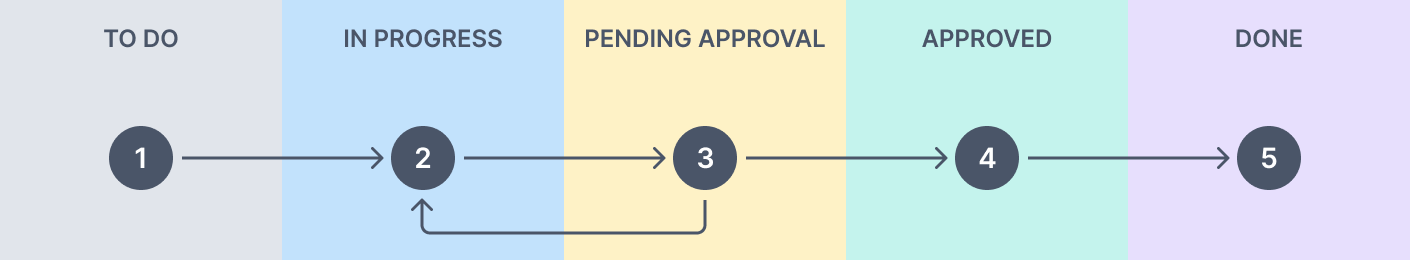
\includegraphics[width=\textwidth]{assets/working-packages/JiraWorkflow.png}
	\caption{5 steps of the Jira workflow}
\end{figure}
All the tasks would have to go from step 1 to step 5 in order to be considered as finished. Each step and the automation is as follows:
\begin{enumerate}
	\item All the tasks that have been selected for the sprint start at the first step, at the \emph{to-do} column.
	\item For each task, a new git branch has to be created with the name of the Jira task tag, for instance \texttt{HBL-185}\footnote{The \texttt{HBL} prefix is assigned when a new Jira project is created.}.
	      \\
	      When the branch is created and pushed to GitHub, Jira will move the task automatically to the \emph{in progress} column. \cite{jira-smart-commits}
	\item While in progress, each commit made is tracked in Jira. Additionally, Jira also supports \emph{smart commits} which are words prefixed with a hash (\#). With the smart commits, task properties can be changed. In this case, only the \texttt{\#time} has been used which increments the amount of time spent in each task. Tracking time has been useful to know more precisely how much time has been spent overall.
	\item Once the task is finished, a new pull request is made which triggers the continuous integration workflows set up at the GitHub repository. These workflows can also be watched by Jira and automate operations in function of the workflow result. If the task does not pass one of the workflows, the task is moved back to the \emph{in progress} tab. Alternatively, if the checks pass, it is moved to the \emph{approved} column.
	\item Finally, in order to be considered \emph{done}, the pull request of the task in question has to be merged. The merge will trigger another automated process which moves the task from \emph{approved} to \emph{done}.
\end{enumerate}
In order to stick to the process as much as possible, tasks moved to \emph{done}, should not be moved back. Instead, a new \emph{bug} type task was created which would start the process again.
\chapter{Framework and previous concepts}
\section{Introduction}
This chapter will cover the knowledge that is required in order to properly develop a booking application. In short terms, it is required to know how\footnote{It is obvious that the may be different implementations, for different gyms. However, the implementation that has been chosen is the one that I thought was most accurate, based on my experience in different gyms.} gyms work, regarding class and room (or non-class) appointments. Furthermore, it is important to have some knowledge on software artchitecture and development, in order to provide value with the application.
\section{Gym overview}
There are few issues to address regarding the appointment system of a gym. In general, there are two types of appointments to be made. The first is the most simple and basic, which is an appointment made to a class or event organized by the gym. Such appointment will have a maximum capacity, for example, the gym may have a fixed number of spinning machines, and it would be nonsense to allow more appointments that spinning bikes are in a spinning class. The second appointment would be an appointment that is made to access the gym for an interval of time. Most gyms have zones in which their clients can access anytime, and exercise themselves using the mahcines or equipment they feel like using. Therefore, the gym has to provide their clients the possibility of accessing their infrastructures within the interval the client wants to work out.
\section{Development overview}
The application will be a web-based application, meaning that it is expected to be used within a browser, accessing a specific URL. Using a web environment completely avoids the native app implementation. One of the most common issues developers face is the fact that, in order to develop an app for different OS, they can rarely use a common code base. Each OS may require a different language or a different implementation, difficulting the addition of new elements or even maintaining the app itself.
\\[8pt]
Therefore, developing an application for the browser removes such issues. That itself does not solve all the problems, as once again there are multiple browsers, all with their different implementation. It appears a new difficulty for developers, who have to know if the application will be cross-browser functional. Nonetheless, most modern browsers have support for JavaScript, which simplifies the development process as the application can be built with the same language, independently of the browser.
\\[8pt]
JavaScript is far from being a perfect language, plus developing a complex application with vanilla JavaScript can be a tough task and very time demanding. Luckily, there exist multiple frameworks which are production-ready and extremely simplify the process of developing applications. One of the most wellknown frameworks is React. React itself does not solve all issues, since, for example, it does not provide a browser routing solution, yet it is simple to understand. Once again, companies or even developers who saw what was React lacking, as the routing solution, started developing what is known as a meta-framework, which is a framework built upon another framework. This is the case of NextJS, a Javascript meta-framework (as it is a React framework), which tries to solve most of React flaws. There exist many more JavaScript frameworks or even other solutions such as WebAssembly, which allows running non-JavaScript applications in browsers. To sum up, a developer whose goal is to create an application for the browser should be comfortable with such concepts.
\\[8pt]
On the other side of the application, there is the persistence layer. The persistence layer is none other that the part of the application that allows the system to \emph{persist} the data of the users. The user will interact with the system, and such interaction will, most likely, output a result. Such result should be stored in the form that the application requires it, as it will add value to the product (it is rarely difficult to find an application that does not have the need of storing any data). It appears a new field of knowledge which is how the data is stored and how such data is exchanged with the client application,
\\[8pt]
Nowadays, there are hundreds of solutions for such problems. Again, it is a matter of convenience when it comes to choosing the languages and databases which will allow the communication and persistence of the data. For the database, it relies on the application type. For example, if the application relies on fast queries, a ram-based database would be a good solution. On the other hand, an application that contains many tables, each with different relationships, such as the one developed in this project, an SQL database would be a better solution. From here, a comparison with the different SQL tools should be made, as each tool has different benefits and drawbacks. Next, the developer would need knowledge in server-client communication. Using a REST API is sometings the go-to solution, however, once again, the server architecture should be chosen taking into account the application requirements and needs. To sum up, the developer should be comfortable knowing different solutions and architectures, in order to find the solution that fits most the application.
\chapter{Requirements specifications}
\section{Introduction}
This chapter will cover the system requirements specification (\emph{SRS}) for the software being developed. The goal of this chapter is to establish the basis for what will be developed, taking into account user needs, functional and non-functional requirements.
\subsection{Purpose}
The application's objective is to provide a simple, scalable and powerful platform to handle gymnasium appointments. Gym owners will be able to create their gym zones and modify the constraints such as total capacity, available hours, and so on. On the other side, gym clients will be able to book an appointment to the gyms they have access to.
\\[8pt]
Therefore, in a single application, gym owners and their workers will be able to control everything that happens inside the gym; while at the same time being able to apply changes and modifications as wanted.
\subsection{Definitions}
There are some definitions to be explained before moving to the next section:
\begin{enumerate}[label = -]
	\item \emph{Gym}. The gym will represent the company overall, not the infrastructure. Such infrastructure is called \emph{virtual gym}.
	\item \emph{Virtual gym}. A virtual gym will be the representation of a gymnasium in the application. A \emph{virtual gym} can have multiple \emph{gym zones}.
	\item \emph{Gym zone}. A gym zone will be the places where clients will book appointments. A more specific definition for gym zones can be found in further sections.
	\item \emph{User}. The \emph{user} is the main person who uses the software. In this case, it is the owner and their workers.
	\item \emph{Template events}. Even though the class concept is explained in further sections, it is important to make a distinction between a \emph{class} and \emph{class template}, \emph{template events} or \emph{template events} (as they are named in the database). On the one hand, events will be assigned to a gym zone and scheduled. On the other hand, \emph{template events} will be used to schedule and link to a zone.
	\item \emph{Archiving} vs \emph{Deleting}. The purpose of archiving anything in the database means it will be stored but not visible. In order to edit it again, the archived element has to be \emph{recovered}. On the other hand, a deleted element will permanently be deleted from the database.
\end{enumerate}
\section{Overall description}
\subsection{Introduction}
This section provides a general explanation about the application, how it is intended to work, the different \emph{personas} to whom it is focused and a brief introduction to the software's functionalities.
\subsection{Product description}
The product will provide a rich interface for the gym owners and their coworkers in order to manage their gym. Managers will create virtual gyms, each of one with different constrains, which will be forwarded to their gym zones. Each gym zone will be of a certain type, for example, a cardio zone, a free-weight zone or even a powerlifting zone. Such and more characteristics will be determined by the workers or who is responsible for the creation of the zones. Once determined the capabilities of each zone, the clients will have the possibility to make their reservations.
\\[8pt]
This software is going to be interesting since it is mainly focused on the managing of appointments. There exist multiple manager systems, some are gym-focused yet there are few that provide an exclusive focus to managing the appointments. It is interesting to have an application that is that specific because most of the companies already have their client management system and other tools. The COVID has changed many things extremely fast and some gymnasiums have not been able to adapt fast enough. That is because using other management tools would mean to change the entire managing software of the company, in order words, starting from zero again. In the future, however, it would be nice to provide a client management system aswell, including subscriptions and so on.
\subsection{User needs}
After having briefly defined the application, two \emph{personas} can be identified: the owner or worker of the gym, and the client.
\\[8pt]
In the following sections, a brief explanation will be given about the functional requirements, yet such requirements will be explained more in depth in later sections.
\subsubsection{Owner or worker}
Such persona needs entire access to the management system, and it is the main user of it. For this persona, the following needs can be defined:
\begin{enumerate}[label = -]
	\item \emph{Ability to create virtual gyms and gym zones}. It is the main purpose of the application. It has to provide all the tools that are required to have an above average managing system.
	\item \emph{Modify virtual gyms and gym zones}. Constraints may change during time. Overall capacity may increase, more cardio machines may be added, and, with these changes, the gym zones will have to adapt to such real life modifications. There has to exist an interface that provides an easy and simple tool to control it.
	\item \emph{Ability to manage clients}. The income of the gym is based on the amount of clients they have, and such clients have to be subscribed into the system. However, the application is not a client management system. It purely focuses on the fact of appointments, yet the client still has to be registered in the application.
	\item \emph{Ability to manage appointments}. The workers have to be able to create, modify or delete the appointments at any time. This process has to be fast and simple, since it is more than usual to have cancellations, clients without reservation, and many more.
	\item \emph{Ability to manage guided events}. Some gym zones will be marked as a guided class zone. Therefore, a schedule will have to be set up for such zone in order to let the user know that.
\end{enumerate}
Furthermore, two user profiles have to be differentiated: the \emph{owner} and the \emph{worker}. The owner needs more control than the worker and some additional needs are\footnote{Some workers may also have access to such capabilities, depending on the permission they have recieved by the owner.}:
\begin{enumerate}[label = -]
	\item \emph{Ability to manage workers}. The owner has to be able to add, remove or update their workers. There must exist an interface that allows such control.
	\item \emph{Ability to manage the privileges of the workers}. In large gymnasium franchises, there may exist different types of workers, each with different tasks. For instance, some may only be able to manage guided sessions, others will manage the client subscriptions and so on. Therefore, a privilege system is required to define a hierarchy in the company.
	\item \emph{Ability to manage gym trainers}. It is important to know what trainers will be responsible for each guided class. For instance, some clients may prefer some trainers than others, when choosing a guided class.
\end{enumerate}
\subsubsection{Client}
The client has little interaction with the system. However, a management application for clients would be pointless if clients could not book their sessions. That is why it will exist another platform to provide access to the client. Such client, will have the following needs:
\begin{enumerate}[label = -]
	\item \emph{Ability to create, modify and delete appointments}. The clients will make the most use of the reservation system. There has to exist a simple and intuitive interface that allows the clients to interact with the system.
	\item \emph{Ability to visualise guided events}. In case the client prefers booking a place for a guided class, it should be able to visualise all the possible events for a day or week, for a zone.
\end{enumerate}
\section{Product functionalities}
The goal of this section is to explain how would the basic flow of the application be. From the owner arranging virtual gyms, the events and assigning the trainers; to the client being able to manage their appointments. By exemplifying the application behavior, it will be easier to determine the functional requirements of the software.
\subsection{Gym}
When registering, the owner will be required to enter the gym information and will be able to customise other information such as the gym contact data. Such settings will be common to all clients and workers, as they will be part of such gym.
\subsection{Virtual gym and gym zones}
The interface has to be intuitive both for the user and the client, while at the same time providing as much utility as possible. Before being able to create appointments, the client needs a place to create such appointments. Therefore, the first mission of the owner is to define each zone. A gym company may have one or more virtual gyms. As stated before, a virtual gym is the representation of the gym infrastructure in the system. Each virtual gym will have different characteristics and information as: the gym location, the total capacity, the opening and closing hours and much more. This virtual gyms can be modified as they may change time to time. If ever needed, the fact of deleting the different virtual gyms will also be possible.
\\[8pt]
Once the virtual gym has been set up, it can have gym zones. Each gym zone will also have its characteristics, most of them similar to the virtual gym ones. However, there is a characteristic that is important to mention: the \emph{type} of the gym zone. Each zone is required a type since some zones may be suitable for events and some not. Such types will be predefined, however the user will have the ability to create their own types. Nonetheless, there will still be the need of distinction between class zones and non-class zones.
\subsection{Events, trainers and workers}
After having defined the structure of the gym, the owner or the workers of the gym can create and schedule events for the different gym zones. Events can not be overlapped in the same zone, yet some events can be scheduled at the same time in different zones. Furthermore, the same class can be done in multiples zones, with different trainers.
\\[8pt]
In order to keep such consistency, the gym owners will create \emph{template events}, which will have specific characteristics. Each template class will be unique, and it will be used to create \emph{events}. In short, the client will create an appointment to a class, which will be a scheduled template class. Nonetheless, appointments will also be required for non-class gym zones, as it is needed to know how many users will access such zone in a certain time. With the explained relation, owners and workers will not have the need to create a class with all the details every single time, rather simply scheduling already created template events.
\\[8pt]
Additionally, a trainer manager system is required. However, a trainer it is a worker as well, only it does not interact with the application. Hence, in the same management view, the owner, and if any worker is allowed to, will be able to create trainers and workers.
\subsection{Clients}
Before continuing, the system still lacks of the main income of the gymnasium: the client. As detailed before, the goal of this application is not to provide a client management system, though it could be a functionality to be implemented in the future. Therefore, the client will also be related to the gym entity.
\\[8pt]
There has to be, definitely, a small client management. However, this management does not need to know about all the information it is kept about the user in the gym. It will only need:
\begin{enumerate}[label = -]
	\item Personal information such as the name, last name and so on. It should include an email to log in to the software.
\end{enumerate}
That is it. From there, the client will have access to another view of the application in which they will be able to make the reservations.
\subsection{Creating appointments}
When the client has been able to connect to the platform, they will be able to visualise the virtual gyms of the gym they belong to. There, the client will see the availability of the different gym zones, the events offered in that zone and other relevant information. From there, they will create their appointments which will be persisted in the system.
\\[8pt]
After the appointment has been made, the client will be able to modify it and remove it, without the need of any explanation.
\section{Functional requirements}
\label{functional-requirements}
\subsection{Introduction}
In this section, the above described requirements will be explained more in depth. The functional requirements are defined as the core functionalities of the system. All requirements exposed in the section are considered essentials and the system would be considered incomplete if it did not satisfy such requisites.
\\[8pt]
The requisites will be exposed with their code name and a number (as \emph{FR-1}), their priority and a brief description. Three levels of priority have been defined:
\begin{enumerate}[label = \arabic{*}.]
	\item \textbf{High priority (3)}. Such requisites must be fulfilled by the application in order to provide a proper user experience.
	\item \textbf{Medium priority (2)}. Such requisites should be fulfilled by the application in order to provide an above average user experience.
	\item \textbf{Low priority (1)}. Such requisites would provide an excellent user experience, yet they are not mandatory.
\end{enumerate}
Furthermore, the overall application will be separated in three different front end applications:
\begin{enumerate}[label = \textbf{\arabic{*}.}]
	\item \textbf{Landing app}. Application which contains the landing application of the product.
	\item \textbf{Core app}. Main application of the product, where the user does most of the work.
	\item \textbf{Appointments app}. Application used by the gym client in order to book their appointments.
\end{enumerate}
\subsection{Landing app - Product information}
The application must have a landing page in which the potential user can find the different features offered by the application.
\begin{enumerate}[label = -]
	\item \textbf{FR-1 (3)}. The user needs to know the different features of the product in a single page.
	\item \textbf{FR-2 (3)}. The user needs to be able to be redirected to the register and login page, from the landing page. Such page is the core page.
	\item \textbf{FR-3 (2)}. The user needs to be able to find a contact page in the landing page and ask for the desired information by providing personal information.
	\item \textbf{FR-4 (3)}. The user needs to find information about the data privacy. No personal data and information is intended to be sold, nor shared.
\end{enumerate}
\subsection{Core app - User registration}
The user, in this case the owner, has to be able to register. In the beginning, the application will be completely free, so the gym owners will have complete access only by registering. A future implementation would be to provide additional features only to the users with a subscription.
\begin{enumerate}[label = -]
	\item \textbf{FR-5 (3)}. The user has to provide personal information in order to register.
	\item \textbf{FR-6 (3)}. The user has to provide information about the gym in order to register.
	\item \textbf{FR-7 (3)}. The user has to provide an email and a password to access the application (log in).
	\item \textbf{FR-8 (3)}. The user needs to be able to see how their data is kept (personal data privacy).
	\item \textbf{FR-9 (1)}. The user should see the information for the different premium and free plans.
	\item \textbf{FR-10 (1)}. The user could have a free trial for the premium features.
\end{enumerate}
\subsection{Core app - Home page}
In the home page view, the user will manage their virtual gyms and gym zones. Furthermore, it will be able to create, update and remove the template events which will be then linked to gym zones schedule.
\subsubsection{Virtual gyms}
The user will enter the home page and will see the list of their virtual gyms. If no virtual gym has been created, they will be asked if they want to create a virtual gym (which will be optional). From the same view, they will be able to create, modify and archive the different virtual gyms, aside from accessing the gym zones of that virtual gym.
\begin{enumerate}[label = -]
	\item \textbf{FR-11 (3)}. The view has to display a list or a grid with the different virtual gyms of the user.
	\item \textbf{FR-12 (3)}. Each virtual gym item has to provide an option to visualise and update all the information of that virtual gym. This means changing both the virtual gym \emph{metadata}, and the virtual gym constraints.
	\item \textbf{FR-13 (3)}. The user has to access the virtual gym view by clicking on a virtual gym.
	\item \textbf{FR-14 (3)}. The user has to access the gym zones view by clicking on a virtual gym.
	\item \textbf{FR-15 (2)}. The user has to be able to search for a virtual gym by its name.
	\item \textbf{FR-16 (1)}. Each virtual gym item has to provide an option to archive that virtual gym (and, consequentially, all the gym zones).
	\item \textbf{FR-17 (1)}. There virtual gym list has to provide an option to programmatically sort the virtual gyms (e.g. by ascending or descending capacity).
	\item \textbf{FR-18 (1)}. There virtual gym list has to provide an option to manually sort the virtual gyms.
\end{enumerate}
\subsubsection{Gym zones}
Once a virtual gym has been created and the user has clicked on the card representing it, the user will be redirected to another view in which the zones of the gym will be displayed. Similarly, as in the virtual gyms view, if the user has not created any gym zone, they will be prompted to do so, if wanted.
\begin{enumerate}[label = -]
	\item \textbf{FR-19 (3)}. The view has to display a list or a grid with the different gym zones of the selected virtual gym.
	\item \textbf{FR-20 (3)}. Each gym zone has to provide an option to visualise and update all the information of that gym zone. This means changing both the gym zone \emph{metadata}, and the gym zone constraints.
	\item \textbf{FR-21 (3)}. The view has to display which zones are class type and wich not.
	\item \textbf{FR-22 (2)}. The user has to see the gym zone view by clicking on it.
	\item \textbf{FR-23 (1)}. Each gym zone has to provide an option to archive the zone.
\end{enumerate}
\subsubsection{Class gym zone schedule}
When the user has created a class gym zone, that zone will have a schedule (or a calendar). Inside this view, the user will be able to see the schedule or calendar from the selected gym zone.
\begin{enumerate}[label = -]
	\item \textbf{FR-24 (3)}. The view has to provide an option to visualise the scheduled events.
	\item \textbf{FR-25 (3)}. From the calendar, the user has to be able to create a guided session (an event template can be used in order to make the process faster). Such \emph{scheduled event} must include: a start and end time, the trainer which will be the guide, a maxiumum capacity and other information.
	\item \textbf{FR-26 (3)}. From the calendar, the user has to be able to create an event.
	\item \textbf{FR-27 (2)}. From the calendar, the user has to be able to see future scheduled events.
	\item \textbf{FR-28 (1)}. From the calendar, the user has to be able to see past scheduled events.
	\item \textbf{FR-29 (1)}. The user has to be able to create guided sessions which are repeated when wanted, from the chosen interval.
	\item \textbf{FR-30 (1)}. After creating a new class on a gym zone, the application has to \emph{recommend} a trainer for that class.
\end{enumerate}
\subsection{Core app - Events page}
Even though this view is simple, it is important to separate the schedule view of a gym zone from the template events. The current view will only provide the necessary tools to create, edit, delete or archive the different event templates.
\begin{enumerate}[label = -]
	\item \textbf{FR-31 (3)}. The user has to be able to see the list of event types of the gym.
	\item \textbf{FR-32 (3)}. There has to be an option in the menu which allows the user to create, update and delete event types.
	\item \textbf{FR-33 (3)}. The user has to be able to see the list of template events of the gym.
	\item \textbf{FR-34 (3)}. There has to be an option in the menu which allows the user to create, update and delete template events.
	\item \textbf{FR-35 (2)}. The user has to be able to archive the event types.
	\item \textbf{FR-36 (1)}. The user has to be able to archive template events.
\end{enumerate}
\subsection{Core app - Workers page}
This view has to allow the user to manage the workers of the gym enterprise and set the different permissions.
\begin{enumerate}[label = -]
	\item \textbf{FR-37 (3)}. The user has to be able to create a new worker, providing personal information and credentials for such worker to user the app. Furthermore, it has to allow the user to set the permissions for that worker.
	\item \textbf{FR-38 (3)}. The same view has to provide an option to update the permissions and the personal information of the worker.
	\item \textbf{FR-39 (3)}. The view has to provide a table to list all the workers.
	\item \textbf{FR-40 (1)}. The user has to be able to set the working hours of each worker.
	\item \textbf{FR-41 (1)}. The view has to provide an input to search the by name, last name or other characteristics the different workers.
\end{enumerate}
\subsection{Core app - Trainers page}
This view has to allow the user to manage the trainers of the gym enterprise.
\begin{enumerate}[label = -]
	\item \textbf{FR-42 (3)}. The user has to be able to create a new trainer, providing personal information and credentials for such worker to user the app.
	\item \textbf{FR-43 (3)}. The same view has to provide an option to update the trainer personal information.
	\item \textbf{FR-44 (3)}. The view has to provide a table list all the trainers.
	\item \textbf{FR-45 (1)}. The user has to be able to set the working hours of each trainer.
	\item \textbf{FR-46 (1)}. The view has to provide an input to search the by name, last name or other characteristics the different trainers.
\end{enumerate}
\subsection{Core app - Clients page}
This view has to allow the user to manage the clients of the gym enterprise.
\begin{enumerate}[label = -]
	\item \textbf{FR-47 (3)}. The user has to be able to create a new client, providing personal information and credentials for such worker to user the app. Alternatively, the client can register himself (\textbf{FR-65}) with a gym code.
	\item \textbf{FR-48 (3)}. The same view has to provide an option to update the client personal information.
	\item \textbf{FR-49 (3)}. The view has to provide a table list all the clients.
	\item \textbf{FR-50 (1)}. The view has to provide an input to search the by name, last name or other characteristics the different clients.
\end{enumerate}
\subsection{Core app - Settings page}
This view has to provide enough settings to customizer the behavior of the behavior and the gym information.
\begin{enumerate}[label = -]
	\item \textbf{FR-51 (3)}. The view has to allow the user to log out.
	\item \textbf{FR-52 (3)}. As an owner, the settings menu has to allow the user to change the gym name and gym characteristics.
	\item \textbf{FR-53 (3)}. As an owner or worker, the settings page has to allow the user to change their personal information.
	\item \textbf{FR-54 (3)}. As an owner or worker, the settings page has to allow the user to change their password.
	\item \textbf{FR-55 (1)}. The settings menu has to provide an option to change the application theme (light and dark) and persist it.
	\item \textbf{FR-56 (1)}. The settings menu has to provide an option to customise the main colours of the user interface.
\end{enumerate}
\subsection{Core app - Analysis page}
The goal of this view is to provide some metrics to \emph{what is happening at the gym}. However, \textbf{as it is not the main purpose of the application}, all the requirements from each will be marked with \emph{low priority}.
\begin{enumerate}[label = -]
	\item \textbf{FR-57 (1)}. The view has to provide a select option to choose what virtual gym wants to be analised.
	\item \textbf{FR-58 (1)}. After having selected a virtual gym, the view has to display in which intervals the virtual gym is most crowded at the current date.
	\item \textbf{FR-59 (1)}. After having selected a virtual gym, the view has to display in which intervals the virtual gym is most crowded during an interval.
	\item \textbf{FR-61 (1)}. After having selected a virtual gym, the view has to display what events will have more clients during an interval.
	\item \textbf{FR-62 (1)}. After having selected a virtual gym, the view has to display what events will have more clients during at the current date.
	\item \textbf{FR-63 (1)}. After having selected a virtual gym, the view has to provide a filter to check what gym zones are more crowded during an interval.
	\item \textbf{FR-64 (1)}. After having selected a virtual gym, the view has to provide a filter to check what gym zones are more crowded at the current date.
\end{enumerate}
\subsection{Client app}
The client application will reuse most of the content from the Core application. However, as it is a client, all the functionalities of modifying and deleting will no appear, as the client does not have access to such views.
\begin{enumerate}[label = -]
	\item \textbf{FR-65 (3)}. The client has to provide personal information and a gym code in order to register.
	\item \textbf{FR-66 (3)}. The client has to provide an email and password to access the application (log in).
	\item \textbf{FR-67 (3)}. The home page has to display a list or a grid with the different virtual gyms of the gym they are subscribed.
	\item \textbf{FR-68 (3)}. On clicking any virtual gym, the home view has to display the gym zones of the selected virtual gym.
	\item \textbf{FR-69 (3)}. The calendar should display the scheduled events, week by week.
	\item \textbf{FR-70 (2)}. On clicking a scheduled event, the client will be able to book a place, if the event is not full.
	\item \textbf{FR-71 (3)}. If the user clicks on a non-class gym zone, a form has to be shown to choose the interval in which they want to make the appointment. This includes the date of the appointment, the duration and the starting hour.
	\item \textbf{FR-72 (3)}. On selecting a date and a duration, the server has to return what available starting hours there are. If there is no capacity for such selections, the user will not be able to create the appointment.
\end{enumerate}
\subsection{Client app - Settings page}
The personal information, which is nearly the settings page for the client, has to display most of their information. Additionally, it can show some user stats \emph{for the geeks}.
\begin{enumerate}[label = -]
	\item \textbf{FR-73 (3)}. The view has to allow the user to log out.
	\item \textbf{FR-74 (3)}. The view has to allow the client to change their personal information.
	\item \textbf{FR-75 (3)}. The view has to allow the client to change their password.
	\item \textbf{FR-76 (3)}. The view has to display a list with all the upcoming appointments of the user.
	\item \textbf{FR-77 (1)}. If wanted, the user has to be able to see a list with all the past appointments.
	\item \textbf{FR-78 (1)}. The settings menu has to provide an option to change the application theme (light and dark) and persist it.
	\item \textbf{FR-79 (1)}. The view has to display an analytics table to see which days have they accessed a virtual gym.
\end{enumerate}
\section{Non-functional requirements}
A non-functional requirement is a requirement that defines system attributes such as security, reliability, maintainability, scalability and usability. Therefore, such requisites do not describe information to keep nor functionalities to implement, rather characteristics of such functionalities. In the system, the following non-functional requirements can be defined:
\begin{enumerate}[label = -]
	\item \textbf{NFR-1 (3)}. The system has to provide a secure authentication method.
	\item \textbf{NFR-2 (2)}. The application has to provide different authentication methods in order to differentiate the gym owner, the gym worker and the gym client.
	\item \textbf{NFR-3 (2)}. The landing and client web applications must provide a responsive interface, so that the application can be seen both in small and large screens.
	\item \textbf{NFR-4 (1)}. The core application has to provide a responsive interface up to a point. In smaller screens such as phones, some functionalities would not be easy to implement nor to use.
	\item \textbf{NFR-5 (2)}. The three web applications have to provide an accessible and semantic HTML structure.
\end{enumerate}
\section{Requirements dependency matrix}
Due to the large quantity of requirements that have been determined for the development of the project, and due to the low relationship between them, the dependencies will be shown individually, in order to avoid displaying a nearly empty table. Using the following notation, the result is more consise and can be understood better.
\\[8pt]
Each dependency will use the following format: \textbf{[FR-1, FR-2, FR-3] \texttt{->} [FR-4, FR-5]}. It states that the functional requirements 1, 2 and 3 depend on the 4 and the 5.
\\[8pt]
\textbf{[FR-11, FR-13, FR-14, FR-16, FR-17, FR-18] \texttt{->} [FR-12]}. In order to visualise, edit or delete a virtual gym, such virtual gym has had to be created previously.
\\[8pt]
\textbf{[FR-19, FR-20, FR-21, FR-22, FR-23] \texttt{->} [FR-12]}. The gym zones are required to exist inside a virtual gym. If such virtual gym has not been created, the user can not visualise, edit or delete the gym zone.
\\[8pt]
\textbf{[FR-19, FR-21, FR-22, FR-23] \texttt{->} [FR-20]}. In order to visualise, edit or delete a gym zone, such gym zone has had to be created previously.
\\[8pt]
\textbf{[FR-24, FR-25, FR-26, FR-27, FR-28, FR-29, FR-30] \texttt{->} [FR-20]}. A calendar is required to exist inside a gym zone. If such gym zone has not been created, the user can not visualise, edit or delete the events of the calendar.
\\[8pt]
\textbf{[FR-31, FR-35] \texttt{->} [FR-32]}. In order to visualise, edit or delete an event type, such event type has had to be created previously.
\\[8pt]
\textbf{[FR-33, FR-36] \texttt{->} [FR-36]}. In order to visualise, edit or delete an event template, such event template has had to be created previously.
\\[8pt]
\textbf{[FR-38, FR-39, FR-40, FR-41] \texttt{->} [FR-27]}. In order to visualise, edit or delete a worker, such worker has had to be created previously.
\\[8pt]
\textbf{[FR-43, FR-44, FR-45, FR-46] \texttt{->} [FR-42]}. In order to visualise, edit or delete a trainer, such trainer has had to be created previously.
\\[8pt]
\textbf{[FR-48, FR-49, FR-50, FR-51] \texttt{->} [FR-47]}. In order to visualise, edit or delete a client, such client has had to be created or registered previously.
\\[8pt]
\textbf{[FR-66, FR-67, FR-68, FR-69, FR-70, FR-71, FR-72] \texttt{->} [FR-65]}. In order to interact with the application, the client must have had registered previously.
\chapter{Planning}
This chapter will cover the planning of the project. After having defined the requirements and the matrix of dependencies of such requirements, working packages will be defined, which will ensure an organized development using tasks.
\section{Working packages}
\label{working-packages}
Each's table corresponds to one of the working packages. Since the \emph{Development} branch of the working packages tree the most extensive, its tables are explained after the \emph{Testing} branch, and so are the package numbers.
\begin{figure}[H]
	\centering
	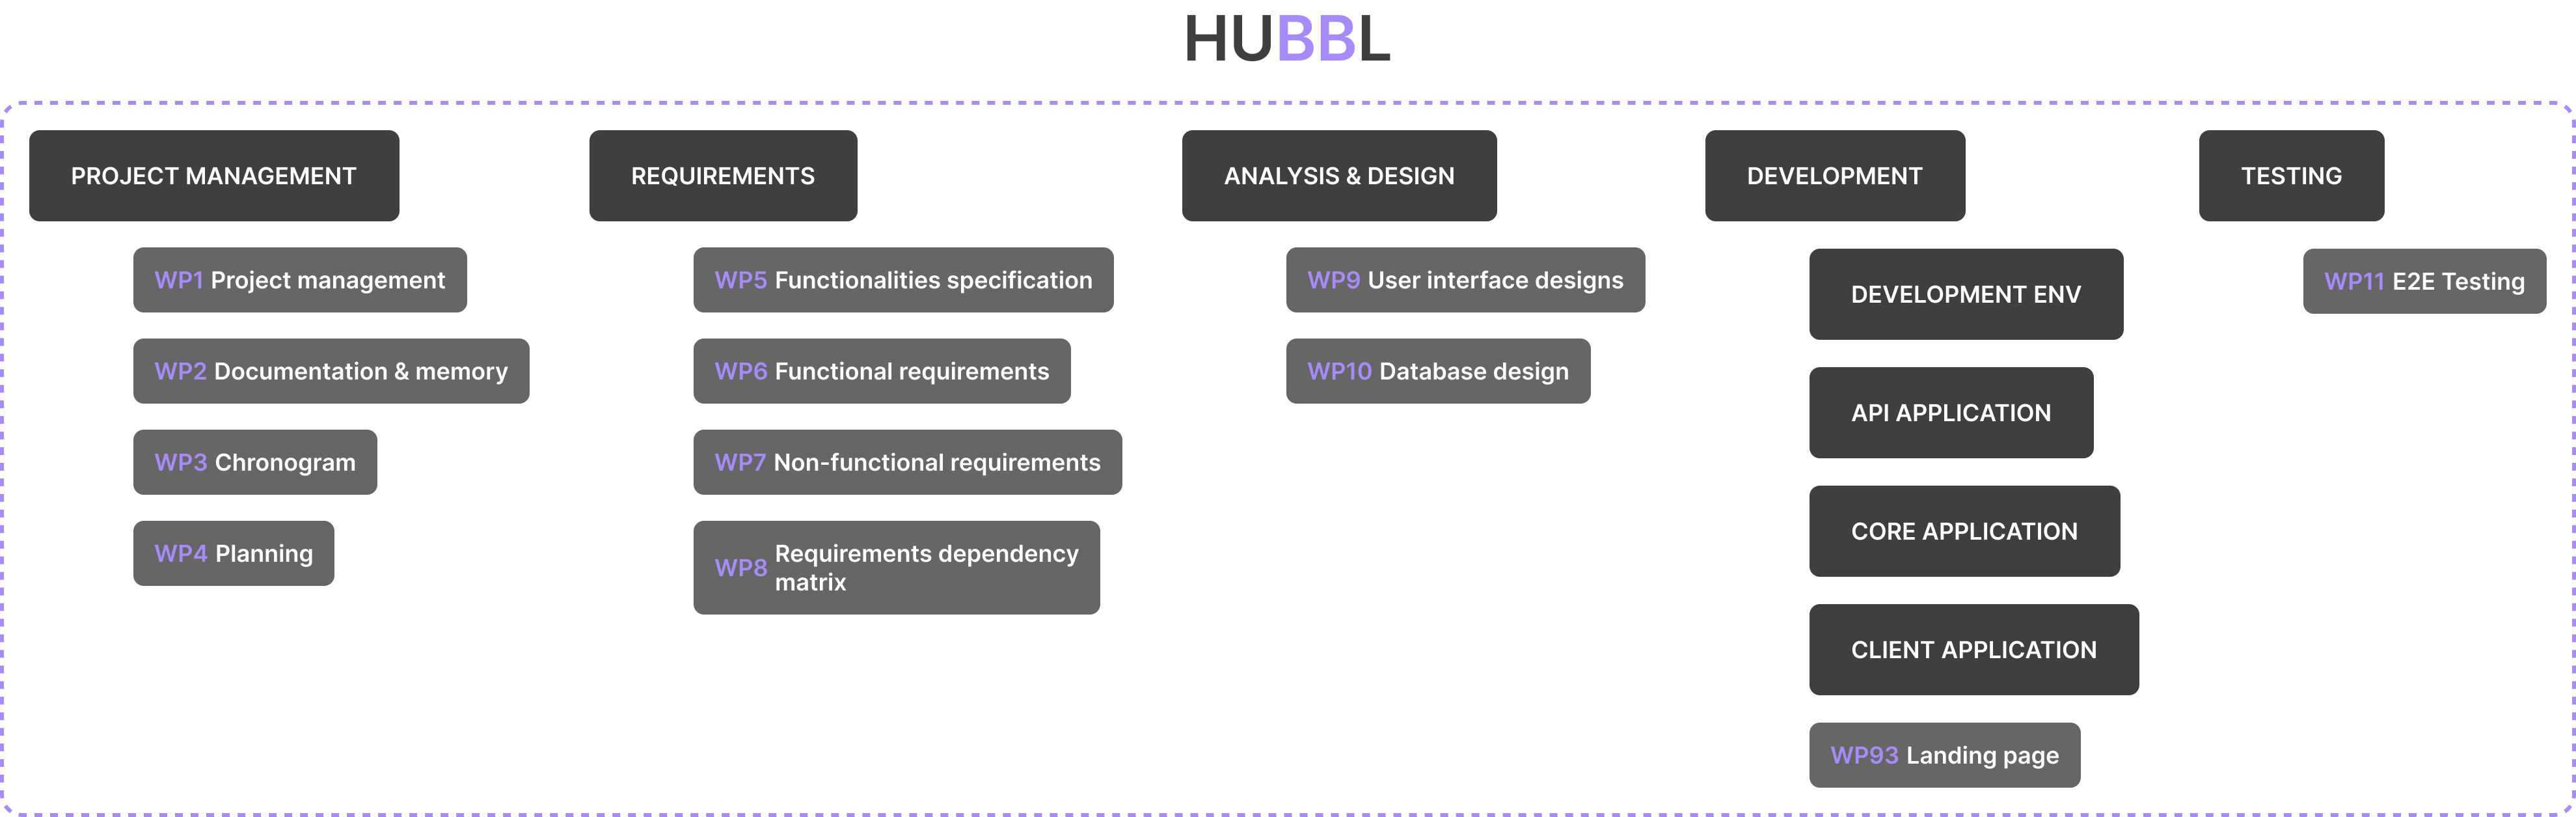
\includegraphics[width=\textwidth]{assets/working-packages/All.png}
	\caption{Structure of the working packages at the root level}
\end{figure}
The image above shows how the working packages have been organized. Each column represents a module, which are:
\begin{enumerate}[label = -]
	\item Project management.
	\item Requirements.
	\item Analysis and design.
	\item Development.
	\item Testing.
\end{enumerate}
Since the development branch is very extensive, each project has been extracted in smaller working packages.
\subsection{Project management}
The \emph{project management} branch contains all the working packages that are related any task that involves the specification of how the project will be managed in order to be successful.
\\[8pt]
\begin{tabularx}{\textwidth}{| l | X |}
	\hline
	\rowcolor{rowColor}
	{\semibf Package name}   & {\semibf WP1}: Project management             \\
	\hline
	{\semibf Description}    & Working package description.                  \\
	\hline
	\rowcolor{rowColor}
	{\semibf Estimated time} & 8h                                            \\
	\hline
	{\semibf Tasks}          & {\semibf T1}: Project document writing.
	\newline {\semibf T2}: Project document review.                          \\
	\hline
	\rowcolor{rowColor}
	{\semibf Results}        & Project document to be submitted to the jury. \\
	\hline
\end{tabularx}
\captionof{table}{Package one's table - Project management}
\vspace*{16pt}
\begin{tabularx}{\textwidth}{| l | X |}
	\hline
	\rowcolor{rowColor}
	{\semibf Package name}   & {\semibf WP2}: Documentation and memory            \\
	\hline
	{\semibf Description}    & Wording of some chapters of the memory.            \\
	\hline
	\rowcolor{rowColor}
	{\semibf Estimated time} & 8h                                                 \\
	\hline
	{\semibf Tasks}          & {\semibf T1}: Wording of the project introduction.
	\newline {\semibf T2}: Wording of the requirements.
	\newline {\semibf T3}: Wording of the analysis and design.
	\newline {\semibf T4}: Wording of the studies and decisions.
	\newline {\semibf T5}: Wording of the project development.                    \\
	\hline
	\rowcolor{rowColor}
	{\semibf Results}        & Project document to be submitted to the jury.      \\
	\hline
\end{tabularx}
\captionof{table}{Package two's table - Documentation and memory}
\vspace*{16pt}
\begin{tabularx}{\textwidth}{| l | X |}
	\hline
	\rowcolor{rowColor}
	{\semibf Package name}   & {\semibf WP3}: Chronogram                                  \\
	\hline
	{\semibf Description}    & Define the working chronogram for the project development. \\
	\hline
	\rowcolor{rowColor}
	{\semibf Estimated time} & 4h                                                         \\
	\hline
	{\semibf Tasks}          & {\semibf T1}: Temporal planning of the working packages.   \\
	\hline
	\rowcolor{rowColor}
	{\semibf Results}        & Gantt's project diagram.                                   \\
	\hline
\end{tabularx}
\captionof{table}{Package three's table - Chronogram}
\vspace*{16pt}
\begin{tabularx}{\textwidth}{| l | X |}
	\hline
	\rowcolor{rowColor}
	{\semibf Package name}   & {\semibf WP4}: Planning                         \\
	\hline
	{\semibf Description}    & Structure the working packages.                 \\
	\hline
	\rowcolor{rowColor}
	{\semibf Estimated time} & 4h                                              \\
	\hline
	{\semibf Tasks}          & {\semibf T1}: Planning of the working packages. \\
	\hline
	\rowcolor{rowColor}
	{\semibf Results}        & Chapter 6 of the memory document.               \\
	\hline
\end{tabularx}
\captionof{table}{Package four's table - Planning}
\vspace*{16pt}
\begin{tabularx}{\textwidth}{| l | X |}
	\hline
	\rowcolor{rowColor}
	{\semibf Package name}   & {\semibf WP5}: Functionalities specification        \\
	\hline
	{\semibf Description}    & Analysis of the functionalities of the application. \\
	\hline
	\rowcolor{rowColor}
	{\semibf Estimated time} & 8h                                                  \\
	\hline
	{\semibf Tasks}          & {\semibf T1}: Users identification.
	\newline {\semibf T2}: Define user needs (owner/worker and client).
	\newline {\semibf T3}: Define product functionalities                          \\
	\hline
	\rowcolor{rowColor}
	{\semibf Results}        & Sections 5.2 and 5.3 of the memory document.        \\
	\hline
\end{tabularx}
\captionof{table}{Package five's table - Functionalities specification}
\subsection{Requirements}
The \emph{requirements} branch contains all the tasks that are related with the analysis and definition of all the requirements and functionalities of each application.
\\[8pt]
\begin{tabularx}{\textwidth}{| l | X |}
	\hline
	\rowcolor{rowColor}
	{\semibf Package name}   & {\semibf WP6}: Functional requirements                                     \\
	\hline
	{\semibf Description}    & Analysis and definition of the functional requirements of the application. \\
	\hline
	\rowcolor{rowColor}
	{\semibf Estimated time} & 12h                                                                        \\
	\hline
	{\semibf Tasks}          & {\semibf T1}: Use case diagram.
	\newline {\semibf T2}: Functional requirements' specification for the \textit{core} application.
	\newline {\semibf T3}: Functional requirements' specification for the \textit{client} application.
	\newline {\semibf T4}: Functional requirements' specification for the \textit{landing} application.
	\newline {\semibf T5}: Functional requirements review and make changes if needed.                     \\
	\hline
	\rowcolor{rowColor}
	{\semibf Results}        & Section 5.4 of the memory document.                                        \\
	\hline
\end{tabularx}
\captionof{table}{Package six's table - Functional requirements}
\vspace*{16pt}
\begin{tabularx}{\textwidth}{| l | X |}
	\hline
	\rowcolor{rowColor}
	{\semibf Package name}   & {\semibf WP7}: Non-functional requirements                                     \\
	\hline
	{\semibf Description}    & Analysis and definition of the non-functional requirements of the application. \\
	\hline
	\rowcolor{rowColor}
	{\semibf Estimated time} & 4h                                                                             \\
	\hline
	{\semibf Tasks}          & {\semibf T1}: Initial non-functional requirements' specification.
	\newline {\semibf T2}: Non-functional requirements review and make changes if needed.                     \\
	\hline
	\rowcolor{rowColor}
	{\semibf Results}        & Section 5.5 of the memory document.                                            \\
	\hline
\end{tabularx}
\captionof{table}{Package seven's table - Non-functional requirements}
\vspace*{16pt}
\begin{tabularx}{\textwidth}{| l | X |}
	\hline
	\rowcolor{rowColor}
	{\semibf Package name}   & {\semibf WP8}: Requirements dependency matrix          \\
	\hline
	{\semibf Description}    & Definition of the requirements' dependency matrix.     \\
	\hline
	\rowcolor{rowColor}
	{\semibf Estimated time} & 4h                                                     \\
	\hline
	{\semibf Tasks}          & {\semibf T1}: Matrix dependency specification once the
	functional and non-functional requirements have been specified.                   \\
	\hline
	\rowcolor{rowColor}
	{\semibf Results}        & Section 5.6 of the memory document.                    \\
	\hline
\end{tabularx}
\captionof{table}{Package eight's table - Requirements dependency matrix}
\subsection{Analysis and design}
The \emph{analysis and design} branch contains all the working packages that are related with the design and analysis of the system interface and architecture.
\\[8pt]
\begin{tabularx}{\textwidth}{| l | X |}
	\hline
	\rowcolor{rowColor}
	{\semibf Package name}   & {\semibf WP9}: User interface designs                                 \\
	\hline
	{\semibf Description}    & Definition of the requirements' dependency matrix.                    \\
	\hline
	\rowcolor{rowColor}
	{\semibf Estimated time} & 96h                                                                   \\
	\hline
	{\semibf Tasks}          & {\semibf T1}: Design system specification.
	\newline {\semibf T2}: Prototype most of the user interfaces.
	\newline {\semibf T3}: Design review. Ensure it satisfies the requirements previously specified. \\
	\hline
	\rowcolor{rowColor}
	{\semibf Results}        & User interface prototypes which provide a vague view of the
	application's look and feel.                                                                     \\
	\hline
\end{tabularx}
\captionof{table}{Package nine's table - User interfaces designs}
\vspace*{16pt}
\begin{tabularx}{\textwidth}{| l | X |}
	\hline
	\rowcolor{rowColor}
	{\semibf Package name}   & {\semibf WP10}: Database design                                       \\
	\hline
	{\semibf Description}    & Definition of the application's database.                             \\
	\hline
	\rowcolor{rowColor}
	{\semibf Estimated time} & 4h                                                                    \\
	\hline
	{\semibf Tasks}          & {\semibf T1}: Design of the applications' database structure.
	\newline {\semibf T2}: Schema and structure review.
	\newline {\semibf T3}: Analysis of the database structure using PostgreSQL.                      \\
	\hline
	\rowcolor{rowColor}
	{\semibf Results}        & Database structure in which the application's data will be persisted. \\
	\hline
\end{tabularx}
\captionof{table}{Package ten - Database design}
\subsection{Testing}
The \emph{testing} branch contains the working package that is related with the testing of the application.
\\[8pt]
\begin{tabularx}{\textwidth}{| l | X |}
	\hline
	\rowcolor{rowColor}
	{\semibf Package name}   & {\semibf WP11}: E2e testing                                              \\
	\hline
	{\semibf Description}    & End-to-end testing implementation for the applications.                  \\
	\hline
	\rowcolor{rowColor}
	{\semibf Estimated time} & 96h                                                                      \\
	\hline
	{\semibf Tasks}          & {\semibf T1}: \emph{API} aplication e2e testing.
	\newline {\semibf T2}: \emph{Core} application e2e testing.
	\newline {\semibf T3}: \emph{Client} application e2e testing.
	\newline {\semibf T4}: \emph{Landing} application e2e testing.                                      \\
	\hline
	\rowcolor{rowColor}
	{\semibf Results}        & End-to-end tests which ensure the correct behaviour of each application,
	and that any futher new features and updates do not break the application.                          \\
	\hline
\end{tabularx}
\captionof{table}{Package eleven's table - E2e testing}
\subsection{Development}
\label{working-packages-development}
The \emph{development} branch is probably the most extensive, as it is the most important part of the project. The branch consists of 73 working packages in total. Nevertheless, most of the packages follow the same structure. For instance, as it is seen in the \emph{\nameref{working-packages-api}}, each web service package follows the same structure: a working package to create an entity, another one to update it, a third one to delete it, and a final one to fetch the entity. The structure is the same for each web service, which easily increases the number of working packages.
\subsubsection{Development env}
The first group that is in the \emph{development} branch is the \emph{development env} (or \emph{development environment}). This part is as important as any other application, since it will define the structure of the project. Furthermore, the continuous integration has to be set up. Using the Nx build system, such feature becomes extremely simple and scalable. One of the options it offers is to run a command to as many projects as wanted. Not only so, that you can run the commands to the affected projects. Such feature reduces even more the CI execution time.
\begin{figure}[H]
	\centering
	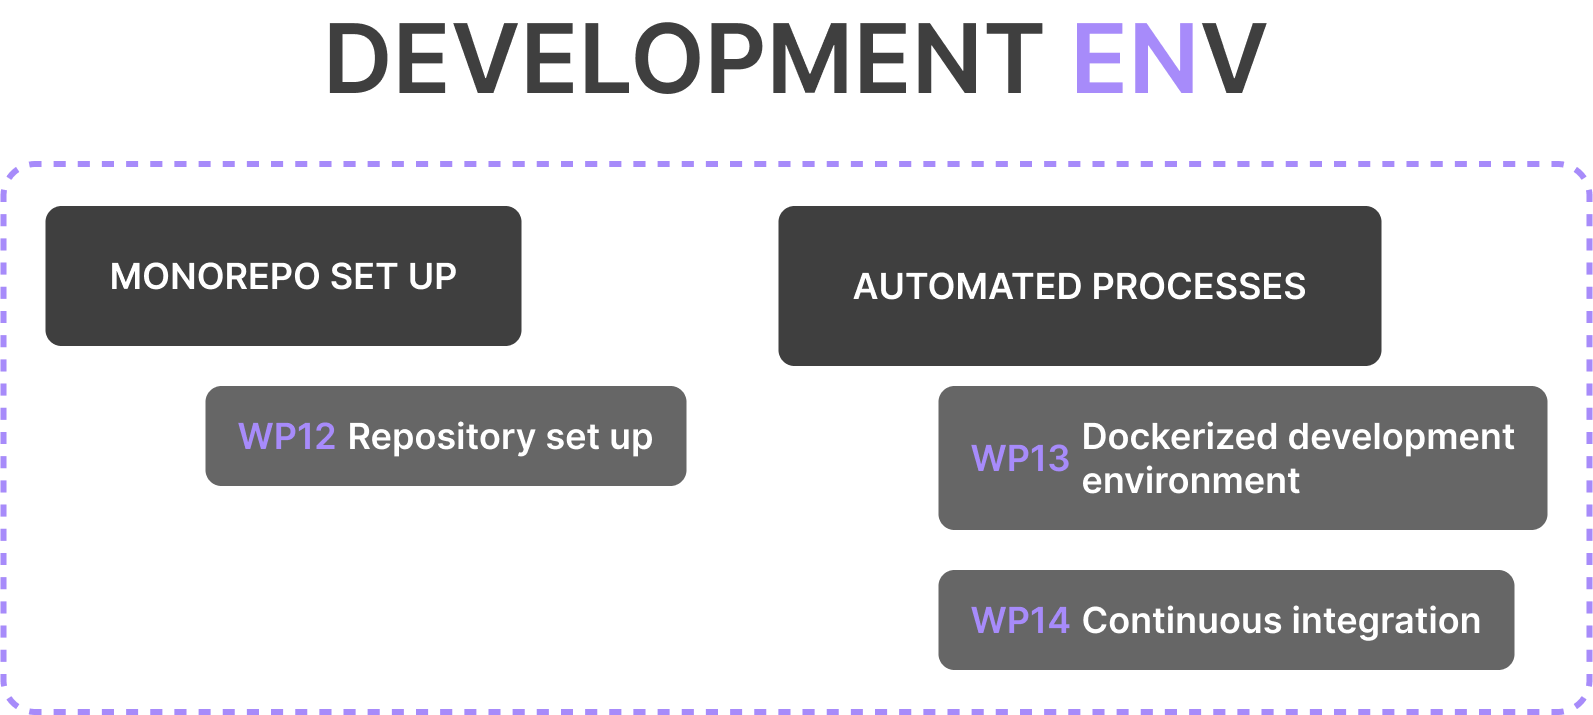
\includegraphics[width=\textwidth]{assets/working-packages/DevEnv.png}
	\caption{Api application working packages diagram}
\end{figure}
The \emph{development environment} group is composed of the following working packages:
\\[8pt]
% region PLANNING_TABLES
\begin{tabularx}{\textwidth}{| l | X |}
	\hline
	\rowcolor{rowColor}
	{\semibf Package name}   & {\semibf WP12}: Repository set up                                 \\
	\hline
	{\semibf Description}    & Prepare the Nx monorepo.                                          \\
	\hline
	\rowcolor{rowColor}
	{\semibf Estimated time} & 4h                                                                \\
	\hline
	{\semibf Tasks}          & {\semibf T1}: Generate an \texttt{nx-workspace} ready to develop. \\
	\hline
	\rowcolor{rowColor}
	{\semibf Results}        & Initial structure of the monorepo.                                \\
	\hline
\end{tabularx}
\captionof{table}{Package twelve's table - Repository set up}
\vspace*{16pt}
\begin{tabularx}{\textwidth}{| l | X |}
	\hline
	\rowcolor{rowColor}
	{\semibf Package name}   & {\semibf WP13}: Dockerized development environment.                \\
	\hline
	{\semibf Description}    & Dockerize the database, the test database and the API application. \\
	\hline
	\rowcolor{rowColor}
	{\semibf Estimated time} & 4h                                                                 \\
	\hline
	{\semibf Tasks}          & {\semibf T1}: Dockerize the main database and the test database.
	\newline {\semibf T2}: Dockerize the API application using a NodeJS image.                    \\
	\hline
	\rowcolor{rowColor}
	{\semibf Results}        & The dockerization of the databases and the REST API.               \\
	\hline
\end{tabularx}
\captionof{table}{Package thirteen's table - Dockerized development environment}
\vspace*{16pt}
\begin{tabularx}{\textwidth}{| l | X |}
	\hline
	\rowcolor{rowColor}
	{\semibf Package name}   & {\semibf WP14}: Continuous integration.                 \\
	\hline
	{\semibf Description}    & Set up Github Actions for CI.                           \\
	\hline
	\rowcolor{rowColor}
	{\semibf Estimated time} & 8h                                                      \\
	\hline
	{\semibf Tasks}          & {\semibf T1}: Set up CI for the \emph{API} application.
	\newline {\semibf T2}: Set up CI for the \emph{core} application.
	\newline {\semibf T3}: Set up CI for the \emph{client} application.
	\newline {\semibf T4}: Set up CI for the \emph{landing} application.
	\newline {\semibf T5}: Set up CI for the monrepo libraries.                        \\
	\hline
	\rowcolor{rowColor}
	{\semibf Results}        & An automated process for testing the code developed.    \\
	\hline
\end{tabularx}
\captionof{table}{Package fourteen's table - Continuous integration}
\subsubsection{Api application}
\label{working-packages-api}
The working package groups of the \emph{api} application have been designed so that each web service of the application is divided in multiple working packages with tasks that are very specific and simple.
\begin{figure}[H]
	\centering
	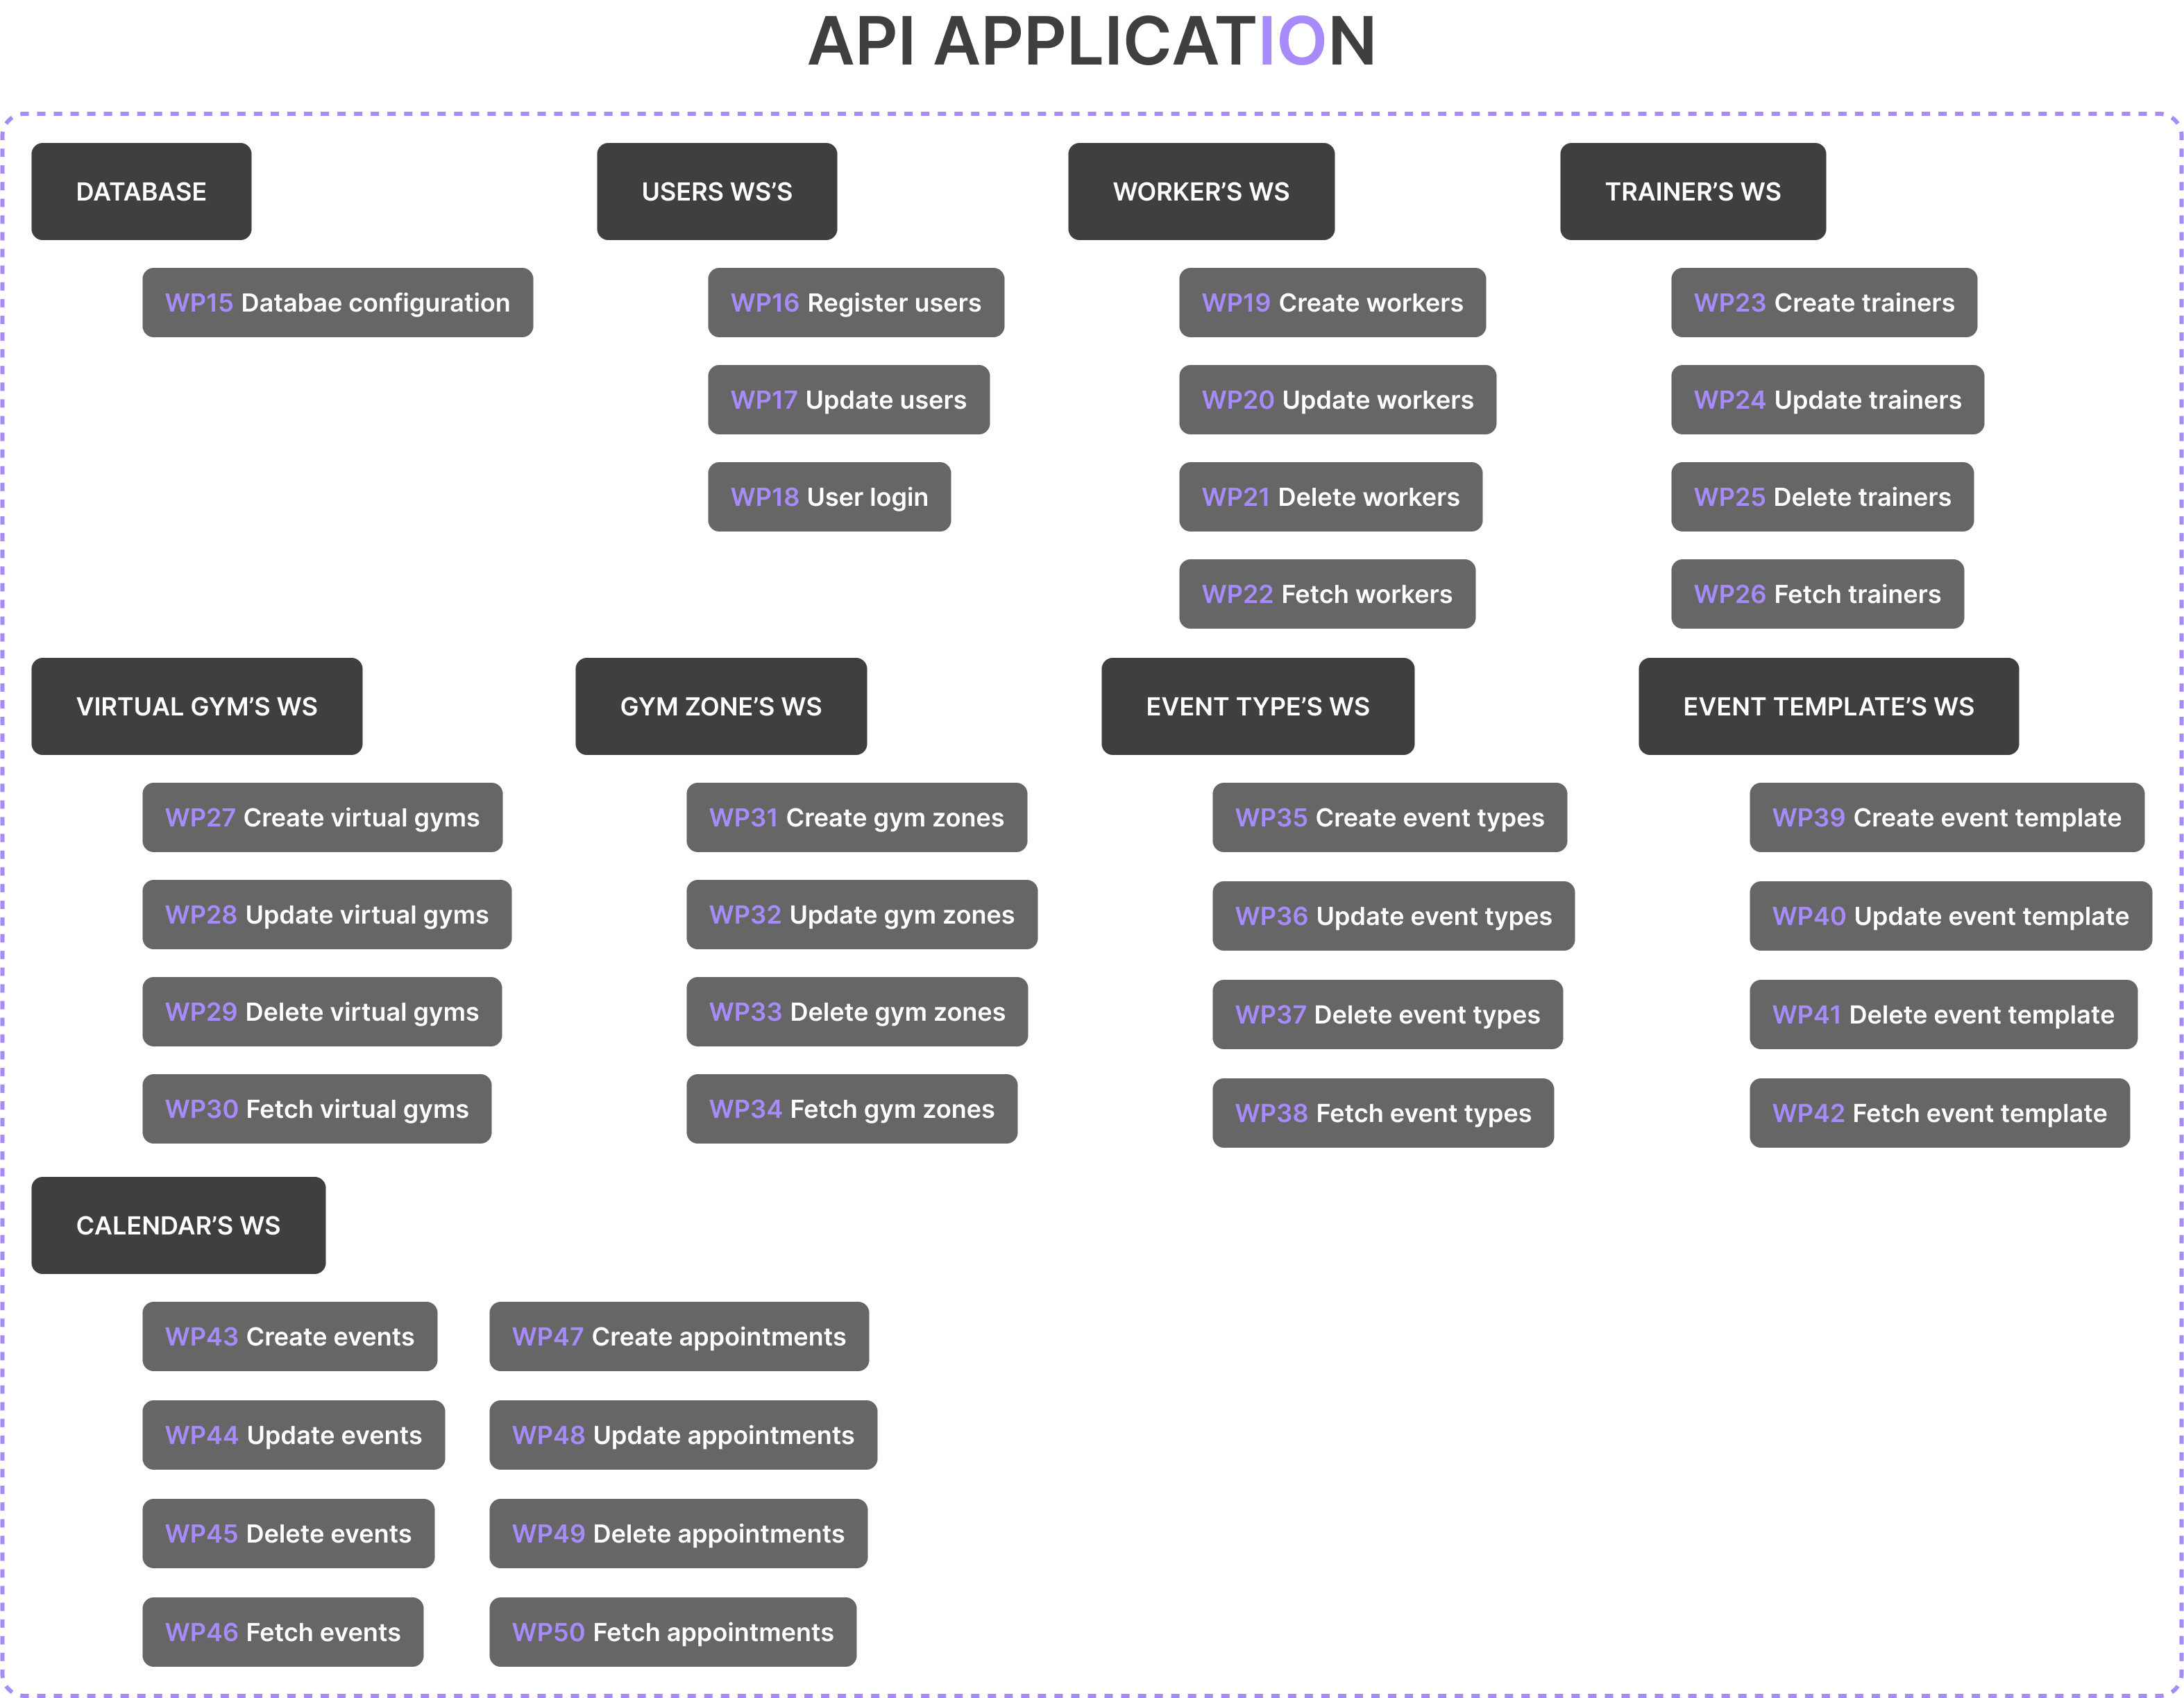
\includegraphics[width=\textwidth]{assets/working-packages/Api.png}
	\caption{Api application working packages diagram}
\end{figure}
The \emph{api} group is composed of the following working packages:
\\[8pt]
\begin{tabularx}{\textwidth}{| l | X |}
	\hline
	\rowcolor{rowColor}
	{\semibf Package name}   & {\semibf WP15}: Database configuration.                       \\
	\hline
	{\semibf Description}    & Configure the application, so that is connected the database. \\
	\hline
	\rowcolor{rowColor}
	{\semibf Estimated time} & 1h                                                            \\
	\hline
	{\semibf Tasks}          & {\semibf T1}: Configure the API with the dockerized database. \\
	\hline
	\rowcolor{rowColor}
	{\semibf Results}        & Connection of the api with the database.                      \\
	\hline
\end{tabularx}
\captionof{table}{Package fifteen's table - Database configuration}
\vspace*{16pt}
\begin{tabularx}{\textwidth}{| l | X |}
	\hline
	\rowcolor{rowColor}
	{\semibf Package name}   & {\semibf WP16}: Register users              \\
	\hline
	{\semibf Description}    & Allow the users to register.                \\
	\hline
	\rowcolor{rowColor}
	{\semibf Estimated time} & 8h                                          \\
	\hline
	{\semibf Tasks}          & {\semibf T1}: Create the services required.
	\newline {\semibf T2}: Create the controllers required.
	\newline {\semibf T3}: Create the owner register endpoint.
	\newline {\semibf T4}: Create the client register endpoint.            \\
	\hline
	\rowcolor{rowColor}
	{\semibf Results}        & Creation of a user.                         \\
	\hline
\end{tabularx}
\captionof{table}{Package sixteen's table - Register users}
\vspace*{16pt}
\begin{tabularx}{\textwidth}{| l | X |}
	\hline
	\rowcolor{rowColor}
	{\semibf Package name}   & {\semibf WP17}: Update users                 \\
	\hline
	{\semibf Description}    & Allow the users to update their information. \\
	\hline
	\rowcolor{rowColor}
	{\semibf Estimated time} & 4h                                           \\
	\hline
	{\semibf Tasks}          & {\semibf T1}: Create the services required.
	\newline {\semibf T2}: Create the controllers required.
	\newline {\semibf T3}: Create the user update endpoint.                 \\
	\hline
	\rowcolor{rowColor}
	{\semibf Results}        & Updation of user's information               \\
	\hline
\end{tabularx}
\captionof{table}{Package seventeen's table - Update users}
\vspace*{16pt}
\begin{tabularx}{\textwidth}{| l | X |}
	\hline
	\rowcolor{rowColor}
	{\semibf Package name}   & {\semibf WP18}: User login                         \\
	\hline
	{\semibf Description}    & Allow the users to log in to the application.      \\
	\hline
	\rowcolor{rowColor}
	{\semibf Estimated time} & 8h                                                 \\
	\hline
	{\semibf Tasks}          & {\semibf T1}: Create the services required.
	\newline {\semibf T2}: Create the controllers required.
	\newline {\semibf T3}: Create the session cookie validation endpoint.
	\newline {\semibf T4}: Create the login endpoint.                             \\
	\hline
	\rowcolor{rowColor}
	{\semibf Results}        & Endpoints to login and validate old user sessions. \\
	\hline
\end{tabularx}
\captionof{table}{Package eighteen's table - User login}
\vspace*{16pt}
\begin{tabularx}{\textwidth}{| l | X |}
	\hline
	\rowcolor{rowColor}
	{\semibf Package name}   & {\semibf WP19}: Create workers              \\
	\hline
	{\semibf Description}    & Allow the creation of workers.              \\
	\hline
	\rowcolor{rowColor}
	{\semibf Estimated time} & 6h                                          \\
	\hline
	{\semibf Tasks}          & {\semibf T1}: Create the services required.
	\newline {\semibf T2}: Create the controllers required.
	\newline {\semibf T3}: Create the workers create endpoint.             \\
	\hline
	\rowcolor{rowColor}
	{\semibf Results}        & Creation of workers.                        \\
	\hline
\end{tabularx}
\captionof{table}{Package nineteen's table - Create workers}
\vspace*{16pt}
\begin{tabularx}{\textwidth}{| l | X |}
	\hline
	\rowcolor{rowColor}
	{\semibf Package name}   & {\semibf WP20}: Update workers              \\
	\hline
	{\semibf Description}    & Allow the update of workers.                \\
	\hline
	\rowcolor{rowColor}
	{\semibf Estimated time} & 4h                                          \\
	\hline
	{\semibf Tasks}          & {\semibf T1}: Create the services required.
	\newline {\semibf T2}: Create the controllers required.
	\newline {\semibf T3}: Create the update workers endpoint.             \\
	\hline
	\rowcolor{rowColor}
	{\semibf Results}        & Updation of workers.                        \\
	\hline
\end{tabularx}
\captionof{table}{Package twenty's table - Update workers}
\vspace*{16pt}
\begin{tabularx}{\textwidth}{| l | X |}
	\hline
	\rowcolor{rowColor}
	{\semibf Package name}   & {\semibf WP21}: Delete workers              \\
	\hline
	{\semibf Description}    & Allow the deletion of workers.              \\
	\hline
	\rowcolor{rowColor}
	{\semibf Estimated time} & 4h                                          \\
	\hline
	{\semibf Tasks}          & {\semibf T1}: Create the services required.
	\newline {\semibf T2}: Create the controllers required.
	\newline {\semibf T3}: Create the delete workers endpoint.             \\
	\hline
	\rowcolor{rowColor}
	{\semibf Results}        & Deletion of workers.                        \\
	\hline
\end{tabularx}
\captionof{table}{Package twenty-one's table - Delete workers}
\vspace*{16pt}
\begin{tabularx}{\textwidth}{| l | X |}
	\hline
	\rowcolor{rowColor}
	{\semibf Package name}   & {\semibf WP22}: Fetch workers               \\
	\hline
	{\semibf Description}    & Allow the fetch of workers.                 \\
	\hline
	\rowcolor{rowColor}
	{\semibf Estimated time} & 4h                                          \\
	\hline
	{\semibf Tasks}          & {\semibf T1}: Create the services required.
	\newline {\semibf T2}: Create the controllers required.
	\newline {\semibf T3}: Create the fetch workers endpoint.              \\
	\hline
	\rowcolor{rowColor}
	{\semibf Results}        & Fetching of workers.                        \\
	\hline
\end{tabularx}
\captionof{table}{Package twenty-two's table - Fetch workers}
\vspace*{16pt}
\begin{tabularx}{\textwidth}{| l | X |}
	\hline
	\rowcolor{rowColor}
	{\semibf Package name}   & {\semibf WP23}: Create trainers             \\
	\hline
	{\semibf Description}    & Allow the creation of trainers.             \\
	\hline
	\rowcolor{rowColor}
	{\semibf Estimated time} & 8h                                          \\
	\hline
	{\semibf Tasks}          & {\semibf T1}: Create the services required.
	\newline {\semibf T2}: Create the controllers required.
	\newline {\semibf T3}: Create the create trainers endpoint.            \\
	\hline
	\rowcolor{rowColor}
	{\semibf Results}        & Creation of trainers.                       \\
	\hline
\end{tabularx}
\captionof{table}{Package twenty-three's table - Create trainers}
\vspace*{16pt}
\begin{tabularx}{\textwidth}{| l | X |}
	\hline
	\rowcolor{rowColor}
	{\semibf Package name}   & {\semibf WP24}: Update trainers             \\
	\hline
	{\semibf Description}    & Allow the update of trainers.               \\
	\hline
	\rowcolor{rowColor}
	{\semibf Estimated time} & 4h                                          \\
	\hline
	{\semibf Tasks}          & {\semibf T1}: Create the services required.
	\newline {\semibf T2}: Create the controllers required.
	\newline {\semibf T3}: Create the update trainers endpoint.            \\
	\hline
	\rowcolor{rowColor}
	{\semibf Results}        & Updation of trainers.                       \\
	\hline
\end{tabularx}
\captionof{table}{Package twenty-four's table - Update trainers}
\vspace*{16pt}
\begin{tabularx}{\textwidth}{| l | X |}
	\hline
	\rowcolor{rowColor}
	{\semibf Package name}   & {\semibf WP25}: Delete trainers             \\
	\hline
	{\semibf Description}    & Allow the deletion of trainers.             \\
	\hline
	\rowcolor{rowColor}
	{\semibf Estimated time} & 4h                                          \\
	\hline
	{\semibf Tasks}          & {\semibf T1}: Create the services required.
	\newline {\semibf T2}: Create the controllers required.
	\newline {\semibf T3}: Create the delete trainers endpoint.            \\
	\hline
	\rowcolor{rowColor}
	{\semibf Results}        & Deletion of trainers.                       \\
	\hline
\end{tabularx}
\captionof{table}{Package twenty-five's table - Delete trainers}
\vspace*{16pt}
\begin{tabularx}{\textwidth}{| l | X |}
	\hline
	\rowcolor{rowColor}
	{\semibf Package name}   & {\semibf WP26}: Fetch trainers              \\
	\hline
	{\semibf Description}    & Allow the fetch of trainers.                \\
	\hline
	\rowcolor{rowColor}
	{\semibf Estimated time} & 4h                                          \\
	\hline
	{\semibf Tasks}          & {\semibf T1}: Create the services required.
	\newline {\semibf T2}: Create the controllers required.
	\newline {\semibf T3}: Create the fetch trainers endpoint.             \\
	\hline
	\rowcolor{rowColor}
	{\semibf Results}        & Fetching of trainers.                       \\
	\hline
\end{tabularx}
\captionof{table}{Package twenty-six's table - Fetch trainers}
\vspace*{16pt}
\begin{tabularx}{\textwidth}{| l | X |}
	\hline
	\rowcolor{rowColor}
	{\semibf Package name}   & {\semibf WP27}: Create virtual gyms         \\
	\hline
	{\semibf Description}    & Allow the creation of virtual gyms.         \\
	\hline
	\rowcolor{rowColor}
	{\semibf Estimated time} & 8h                                          \\
	\hline
	{\semibf Tasks}          & {\semibf T1}: Create the services required.
	\newline {\semibf T2}: Create the controllers required.
	\newline {\semibf T3}: Create the virtual gym creation endpoint.       \\
	\hline
	\rowcolor{rowColor}
	{\semibf Results}        & Creation of virtual gyms.                   \\
	\hline
\end{tabularx}
\captionof{table}{Package twenty-seven's table - Create virtual gyms}
\vspace*{16pt}
\begin{tabularx}{\textwidth}{| l | X |}
	\hline
	\rowcolor{rowColor}
	{\semibf Package name}   & {\semibf WP28}: Update virtual gyms         \\
	\hline
	{\semibf Description}    & Allow the update of virtual gyms.           \\
	\hline
	\rowcolor{rowColor}
	{\semibf Estimated time} & 4h                                          \\
	\hline
	{\semibf Tasks}          & {\semibf T1}: Create the services required.
	\newline {\semibf T2}: Create the controllers required.
	\newline {\semibf T3}: Create the virtual gym update endpoint.         \\
	\hline
	\rowcolor{rowColor}
	{\semibf Results}        & Updation of virtual gyms.                   \\
	\hline
\end{tabularx}
\captionof{table}{Package twenty-eight's table - Update virtual gyms}
\vspace*{16pt}
\begin{tabularx}{\textwidth}{| l | X |}
	\hline
	\rowcolor{rowColor}
	{\semibf Package name}   & {\semibf WP29}: Delete virtual gyms         \\
	\hline
	{\semibf Description}    & Allow the deletion of virtual gyms.         \\
	\hline
	\rowcolor{rowColor}
	{\semibf Estimated time} & 4h                                          \\
	\hline
	{\semibf Tasks}          & {\semibf T1}: Create the services required.
	\newline {\semibf T2}: Create the controllers required.
	\newline {\semibf T3}: Create the virtual gym deletion endpoint.       \\
	\hline
	\rowcolor{rowColor}
	{\semibf Results}        & Deletion of virtual gyms.                   \\
	\hline
\end{tabularx}
\captionof{table}{Package twenty-nine's table - Delete virtual gyms}
\vspace*{16pt}
\begin{tabularx}{\textwidth}{| l | X |}
	\hline
	\rowcolor{rowColor}
	{\semibf Package name}   & {\semibf WP30}: Fetch virtual gyms          \\
	\hline
	{\semibf Description}    & Allow the fetch of virtual gyms.            \\
	\hline
	\rowcolor{rowColor}
	{\semibf Estimated time} & 4h                                          \\
	\hline
	{\semibf Tasks}          & {\semibf T1}: Create the services required.
	\newline {\semibf T2}: Create the controllers required.
	\newline {\semibf T3}: Create the virtual gym fetch endpoint.          \\
	\hline
	\rowcolor{rowColor}
	{\semibf Results}        & Fetching of virtual gyms.                   \\
	\hline
\end{tabularx}
\captionof{table}{Package thirty's table - Delete virtual gyms}
\vspace*{16pt}
\begin{tabularx}{\textwidth}{| l | X |}
	\hline
	\rowcolor{rowColor}
	{\semibf Package name}   & {\semibf WP31}: Create gym zones            \\
	\hline
	{\semibf Description}    & Allow the creation of gym zones.            \\
	\hline
	\rowcolor{rowColor}
	{\semibf Estimated time} & 8h                                          \\
	\hline
	{\semibf Tasks}          & {\semibf T1}: Create the services required.
	\newline {\semibf T2}: Create the controllers required.
	\newline {\semibf T3}: Create the gym zone create endpoint.            \\
	\hline
	\rowcolor{rowColor}
	{\semibf Results}        & Creation of gym zones.                      \\
	\hline
\end{tabularx}
\captionof{table}{Package thirty-one's table - Create gym zones}
\vspace*{16pt}
\begin{tabularx}{\textwidth}{| l | X |}
	\hline
	\rowcolor{rowColor}
	{\semibf Package name}   & {\semibf WP32}: Update gym zones            \\
	\hline
	{\semibf Description}    & Allow the update of gym zones.              \\
	\hline
	\rowcolor{rowColor}
	{\semibf Estimated time} & 4h                                          \\
	\hline
	{\semibf Tasks}          & {\semibf T1}: Create the services required.
	\newline {\semibf T2}: Create the controllers required.
	\newline {\semibf T3}: Create the gym zone update endpoint.            \\
	\hline
	\rowcolor{rowColor}
	{\semibf Results}        & Updation of gym zones.                      \\
	\hline
\end{tabularx}
\captionof{table}{Package thirty-two's table - Update gym zones}
\vspace*{16pt}
\begin{tabularx}{\textwidth}{| l | X |}
	\hline
	\rowcolor{rowColor}
	{\semibf Package name}   & {\semibf WP33}: Delete gym zones            \\
	\hline
	{\semibf Description}    & Allow the deletion of gym zones.            \\
	\hline
	\rowcolor{rowColor}
	{\semibf Estimated time} & 4h                                          \\
	\hline
	{\semibf Tasks}          & {\semibf T1}: Create the services required.
	\newline {\semibf T2}: Create the controllers required.
	\newline {\semibf T3}: Create the gym zone delete endpoint.            \\
	\hline
	\rowcolor{rowColor}
	{\semibf Results}        & Deletion of gym zones.                      \\
	\hline
\end{tabularx}
\captionof{table}{Package thirty-three's table - Delete gym zones}
\vspace*{16pt}
\begin{tabularx}{\textwidth}{| l | X |}
	\hline
	\rowcolor{rowColor}
	{\semibf Package name}   & {\semibf WP34}: Fetch gym zones             \\
	\hline
	{\semibf Description}    & Allow the fetching of gym zones.            \\
	\hline
	\rowcolor{rowColor}
	{\semibf Estimated time} & 4h                                          \\
	\hline
	{\semibf Tasks}          & {\semibf T1}: Create the services required.
	\newline {\semibf T2}: Create the controllers required.
	\newline {\semibf T3}: Create the gym zone fetch endpoint.             \\
	\hline
	\rowcolor{rowColor}
	{\semibf Results}        & Fetching of gym zones.                      \\
	\hline
\end{tabularx}
\captionof{table}{Package thirty-four's table - Fetch gym zones}
\vspace*{16pt}
\begin{tabularx}{\textwidth}{| l | X |}
	\hline
	\rowcolor{rowColor}
	{\semibf Package name}   & {\semibf WP35}: Create event types          \\
	\hline
	{\semibf Description}    & Allow the creation of event types.          \\
	\hline
	\rowcolor{rowColor}
	{\semibf Estimated time} & 8h                                          \\
	\hline
	{\semibf Tasks}          & {\semibf T1}: Create the services required.
	\newline {\semibf T2}: Create the controllers required.
	\newline {\semibf T3}: Create the event types create endpoint.         \\
	\hline
	\rowcolor{rowColor}
	{\semibf Results}        & Creation of event types.                    \\
	\hline
\end{tabularx}
\captionof{table}{Package thirty-five's table - Create event types}
\vspace*{16pt}
\begin{tabularx}{\textwidth}{| l | X |}
	\hline
	\rowcolor{rowColor}
	{\semibf Package name}   & {\semibf WP36}: Update event types          \\
	\hline
	{\semibf Description}    & Allow the update of event types.            \\
	\hline
	\rowcolor{rowColor}
	{\semibf Estimated time} & 4h                                          \\
	\hline
	{\semibf Tasks}          & {\semibf T1}: Create the services required.
	\newline {\semibf T2}: Create the controllers required.
	\newline {\semibf T3}: Create the event types update endpoint.         \\
	\hline
	\rowcolor{rowColor}
	{\semibf Results}        & Updation of event types.                    \\
	\hline
\end{tabularx}
\captionof{table}{Package thirty-six's table - Update event types}
\vspace*{16pt}
\begin{tabularx}{\textwidth}{| l | X |}
	\hline
	\rowcolor{rowColor}
	{\semibf Package name}   & {\semibf WP37}: Delete event types          \\
	\hline
	{\semibf Description}    & Allow the deletion of event types.          \\
	\hline
	\rowcolor{rowColor}
	{\semibf Estimated time} & 4h                                          \\
	\hline
	{\semibf Tasks}          & {\semibf T1}: Create the services required.
	\newline {\semibf T2}: Create the controllers required.
	\newline {\semibf T3}: Create the event types delete endpoint.         \\
	\hline
	\rowcolor{rowColor}
	{\semibf Results}        & Updation of event types.                    \\
	\hline
\end{tabularx}
\captionof{table}{Package thirty-seven's table - Delete event types}
\vspace*{16pt}
\begin{tabularx}{\textwidth}{| l | X |}
	\hline
	\rowcolor{rowColor}
	{\semibf Package name}   & {\semibf WP38}: Fetch event types           \\
	\hline
	{\semibf Description}    & Allow the fetch of event types.             \\
	\hline
	\rowcolor{rowColor}
	{\semibf Estimated time} & 4h                                          \\
	\hline
	{\semibf Tasks}          & {\semibf T1}: Create the services required.
	\newline {\semibf T2}: Create the controllers required.
	\newline {\semibf T3}: Create the event types fetch endpoint.          \\
	\hline
	\rowcolor{rowColor}
	{\semibf Results}        & Fetching of event types.                    \\
	\hline
\end{tabularx}
\captionof{table}{Package thirty-eight's table - Fetch event types}
\vspace*{16pt}
\begin{tabularx}{\textwidth}{| l | X |}
	\hline
	\rowcolor{rowColor}
	{\semibf Package name}   & {\semibf WP39}: Create event templates      \\
	\hline
	{\semibf Description}    & Allow the creation of event templates.      \\
	\hline
	\rowcolor{rowColor}
	{\semibf Estimated time} & 4h                                          \\
	\hline
	{\semibf Tasks}          & {\semibf T1}: Create the services required.
	\newline {\semibf T2}: Create the controllers required.
	\newline {\semibf T3}: Create the event templates create endpoint.     \\
	\hline
	\rowcolor{rowColor}
	{\semibf Results}        & Creation of event templates.                \\
	\hline
\end{tabularx}
\captionof{table}{Package thirty-nine's table - Create event templates}
\vspace*{16pt}
\begin{tabularx}{\textwidth}{| l | X |}
	\hline
	\rowcolor{rowColor}
	{\semibf Package name}   & {\semibf WP40}: Update event templates      \\
	\hline
	{\semibf Description}    & Allow the update of event templates.        \\
	\hline
	\rowcolor{rowColor}
	{\semibf Estimated time} & 4h                                          \\
	\hline
	{\semibf Tasks}          & {\semibf T1}: Create the services required.
	\newline {\semibf T2}: Create the controllers required.
	\newline {\semibf T3}: Create the event templates update endpoint.     \\
	\hline
	\rowcolor{rowColor}
	{\semibf Results}        & Updation of event templates.                \\
	\hline
\end{tabularx}
\captionof{table}{Package forty's table - Update event templates}
\vspace*{16pt}
\begin{tabularx}{\textwidth}{| l | X |}
	\hline
	\rowcolor{rowColor}
	{\semibf Package name}   & {\semibf WP41}: Delete event templates      \\
	\hline
	{\semibf Description}    & Allow the deletion of event templates.      \\
	\hline
	\rowcolor{rowColor}
	{\semibf Estimated time} & 4h                                          \\
	\hline
	{\semibf Tasks}          & {\semibf T1}: Create the services required.
	\newline {\semibf T2}: Create the controllers required.
	\newline {\semibf T3}: Create the event templates delete endpoint.     \\
	\hline
	\rowcolor{rowColor}
	{\semibf Results}        & Deletion of event templates.                \\
	\hline
\end{tabularx}
\captionof{table}{Package forty-one's table - Delete event templates}
\vspace*{16pt}
\begin{tabularx}{\textwidth}{| l | X |}
	\hline
	\rowcolor{rowColor}
	{\semibf Package name}   & {\semibf WP42}: Fetch event templates       \\
	\hline
	{\semibf Description}    & Allow the fetch of event templates.         \\
	\hline
	\rowcolor{rowColor}
	{\semibf Estimated time} & 4h                                          \\
	\hline
	{\semibf Tasks}          & {\semibf T1}: Create the services required.
	\newline {\semibf T2}: Create the controllers required.
	\newline {\semibf T3}: Create the event templates fetch endpoint.      \\
	\hline
	\rowcolor{rowColor}
	{\semibf Results}        & Fetching of event templates.                \\
	\hline
\end{tabularx}
\captionof{table}{Package forty-two's table - Fetch event templates}
\vspace*{16pt}
\begin{tabularx}{\textwidth}{| l | X |}
	\hline
	\rowcolor{rowColor}
	{\semibf Package name}   & {\semibf WP43}: Create events               \\
	\hline
	{\semibf Description}    & Allow the creation of events.               \\
	\hline
	\rowcolor{rowColor}
	{\semibf Estimated time} & 8h                                          \\
	\hline
	{\semibf Tasks}          & {\semibf T1}: Create the services required.
	\newline {\semibf T2}: Create the controllers required.
	\newline {\semibf T3}: Create the events fetch endpoint.               \\
	\hline
	\rowcolor{rowColor}
	{\semibf Results}        & Creation of events.                         \\
	\hline
\end{tabularx}
\captionof{table}{Package forty-three's table - Create events}
\vspace*{16pt}
\begin{tabularx}{\textwidth}{| l | X |}
	\hline
	\rowcolor{rowColor}
	{\semibf Package name}   & {\semibf WP44}: Update events               \\
	\hline
	{\semibf Description}    & Allow the update of events.                 \\
	\hline
	\rowcolor{rowColor}
	{\semibf Estimated time} & 4h                                          \\
	\hline
	{\semibf Tasks}          & {\semibf T1}: Create the services required.
	\newline {\semibf T2}: Create the controllers required.
	\newline {\semibf T3}: Create the events update endpoint.              \\
	\hline
	\rowcolor{rowColor}
	{\semibf Results}        & Updation of events.                         \\
	\hline
\end{tabularx}
\captionof{table}{Package forty-four's table - Update events}
\vspace*{16pt}
\begin{tabularx}{\textwidth}{| l | X |}
	\hline
	\rowcolor{rowColor}
	{\semibf Package name}   & {\semibf WP45}: Delete events               \\
	\hline
	{\semibf Description}    & Allow the deletion of events.               \\
	\hline
	\rowcolor{rowColor}
	{\semibf Estimated time} & 4h                                          \\
	\hline
	{\semibf Tasks}          & {\semibf T1}: Create the services required.
	\newline {\semibf T2}: Create the controllers required.
	\newline {\semibf T3}: Create the events delete endpoint.              \\
	\hline
	\rowcolor{rowColor}
	{\semibf Results}        & Deletion of events.                         \\
	\hline
\end{tabularx}
\captionof{table}{Package forty-five's table - Delete events}
\vspace*{16pt}
\begin{tabularx}{\textwidth}{| l | X |}
	\hline
	\rowcolor{rowColor}
	{\semibf Package name}   & {\semibf WP46}: Fetch events                \\
	\hline
	{\semibf Description}    & Allow the fetching of events.               \\
	\hline
	\rowcolor{rowColor}
	{\semibf Estimated time} & 4h                                          \\
	\hline
	{\semibf Tasks}          & {\semibf T1}: Create the services required.
	\newline {\semibf T2}: Create the controllers required.
	\newline {\semibf T3}: Create the events fetch endpoint.               \\
	\hline
	\rowcolor{rowColor}
	{\semibf Results}        & Fetching of events.                         \\
	\hline
\end{tabularx}
\captionof{table}{Package forty-six's table - Fetch events}
\vspace*{16pt}
\begin{tabularx}{\textwidth}{| l | X |}
	\hline
	\rowcolor{rowColor}
	{\semibf Package name}   & {\semibf WP47}: Create appointments                                             \\
	\hline
	{\semibf Description}    & Allow the fetching of appointments. It is important to create an algorithm that
	ensures that a gym zone does not have more appointments than its capacity.                                 \\
	\hline
	\rowcolor{rowColor}
	{\semibf Estimated time} & 16h                                                                             \\
	\hline
	{\semibf Tasks}          & {\semibf T1}: Create the services required.
	\newline {\semibf T2}: Create the controllers required.
	\newline {\semibf T3}: Create the available hours endpoint.
	\newline {\semibf T4}: Create the appointments create endpoint.                                            \\
	\hline
	\rowcolor{rowColor}
	{\semibf Results}        & Creation of appointments.                                                       \\
	\hline
\end{tabularx}
\captionof{table}{Package forty-seven's table - Create appointments}
\vspace*{16pt}
\begin{tabularx}{\textwidth}{| l | X |}
	\hline
	\rowcolor{rowColor}
	{\semibf Package name}   & {\semibf WP48}: Update appointments                              \\
	\hline
	{\semibf Description}    & Allow the update of appointments. It should only allow to cancel
	the appointment.                                                                            \\
	\hline
	\rowcolor{rowColor}
	{\semibf Estimated time} & 4h                                                               \\
	\hline
	{\semibf Tasks}          & {\semibf T1}: Create the services required.
	\newline {\semibf T2}: Create the controllers required.
	\newline {\semibf T4}: Create the appointments update endpoint.                             \\
	\hline
	\rowcolor{rowColor}
	{\semibf Results}        & Updation of appointments.                                        \\
	\hline
\end{tabularx}
\captionof{table}{Package forty-eight's table - Update appointments}
\vspace*{16pt}
\begin{tabularx}{\textwidth}{| l | X |}
	\hline
	\rowcolor{rowColor}
	{\semibf Package name}   & {\semibf WP49}: Delete appointments                                \\
	\hline
	{\semibf Description}    & Allow the deletion of appointments. It should only allow to cancel
	the appointment.                                                                              \\
	\hline
	\rowcolor{rowColor}
	{\semibf Estimated time} & 4h                                                                 \\
	\hline
	{\semibf Tasks}          & {\semibf T1}: Create the services required.
	\newline {\semibf T2}: Create the controllers required.
	\newline {\semibf T4}: Create the appointments delete endpoint.                               \\
	\hline
	\rowcolor{rowColor}
	{\semibf Results}        & Deletion of appointments.                                          \\
	\hline
\end{tabularx}
\captionof{table}{Package forty-nine's table - Delete appointments}
\vspace*{16pt}
\begin{tabularx}{\textwidth}{| l | X |}
	\hline
	\rowcolor{rowColor}
	{\semibf Package name}   & {\semibf WP50}: Fetch appointments          \\
	\hline
	{\semibf Description}    & Allow the fetch of appointments.            \\
	\hline
	\rowcolor{rowColor}
	{\semibf Estimated time} & 6h                                          \\
	\hline
	{\semibf Tasks}          & {\semibf T1}: Create the services required.
	\newline {\semibf T2}: Create the controllers required.
	\newline {\semibf T4}: Create the appointments fetch endpoint.         \\
	\hline
	\rowcolor{rowColor}
	{\semibf Results}        & Fetching of appointments.                   \\
	\hline
\end{tabularx}
\captionof{table}{Package fifty's table - Fetch appointments}
\subsubsection{Core application}
The \emph{core} group of working packages follows a similar approach as the one described in \emph{\nameref{working-packages-development}}.
\begin{figure}[H]
	\centering
	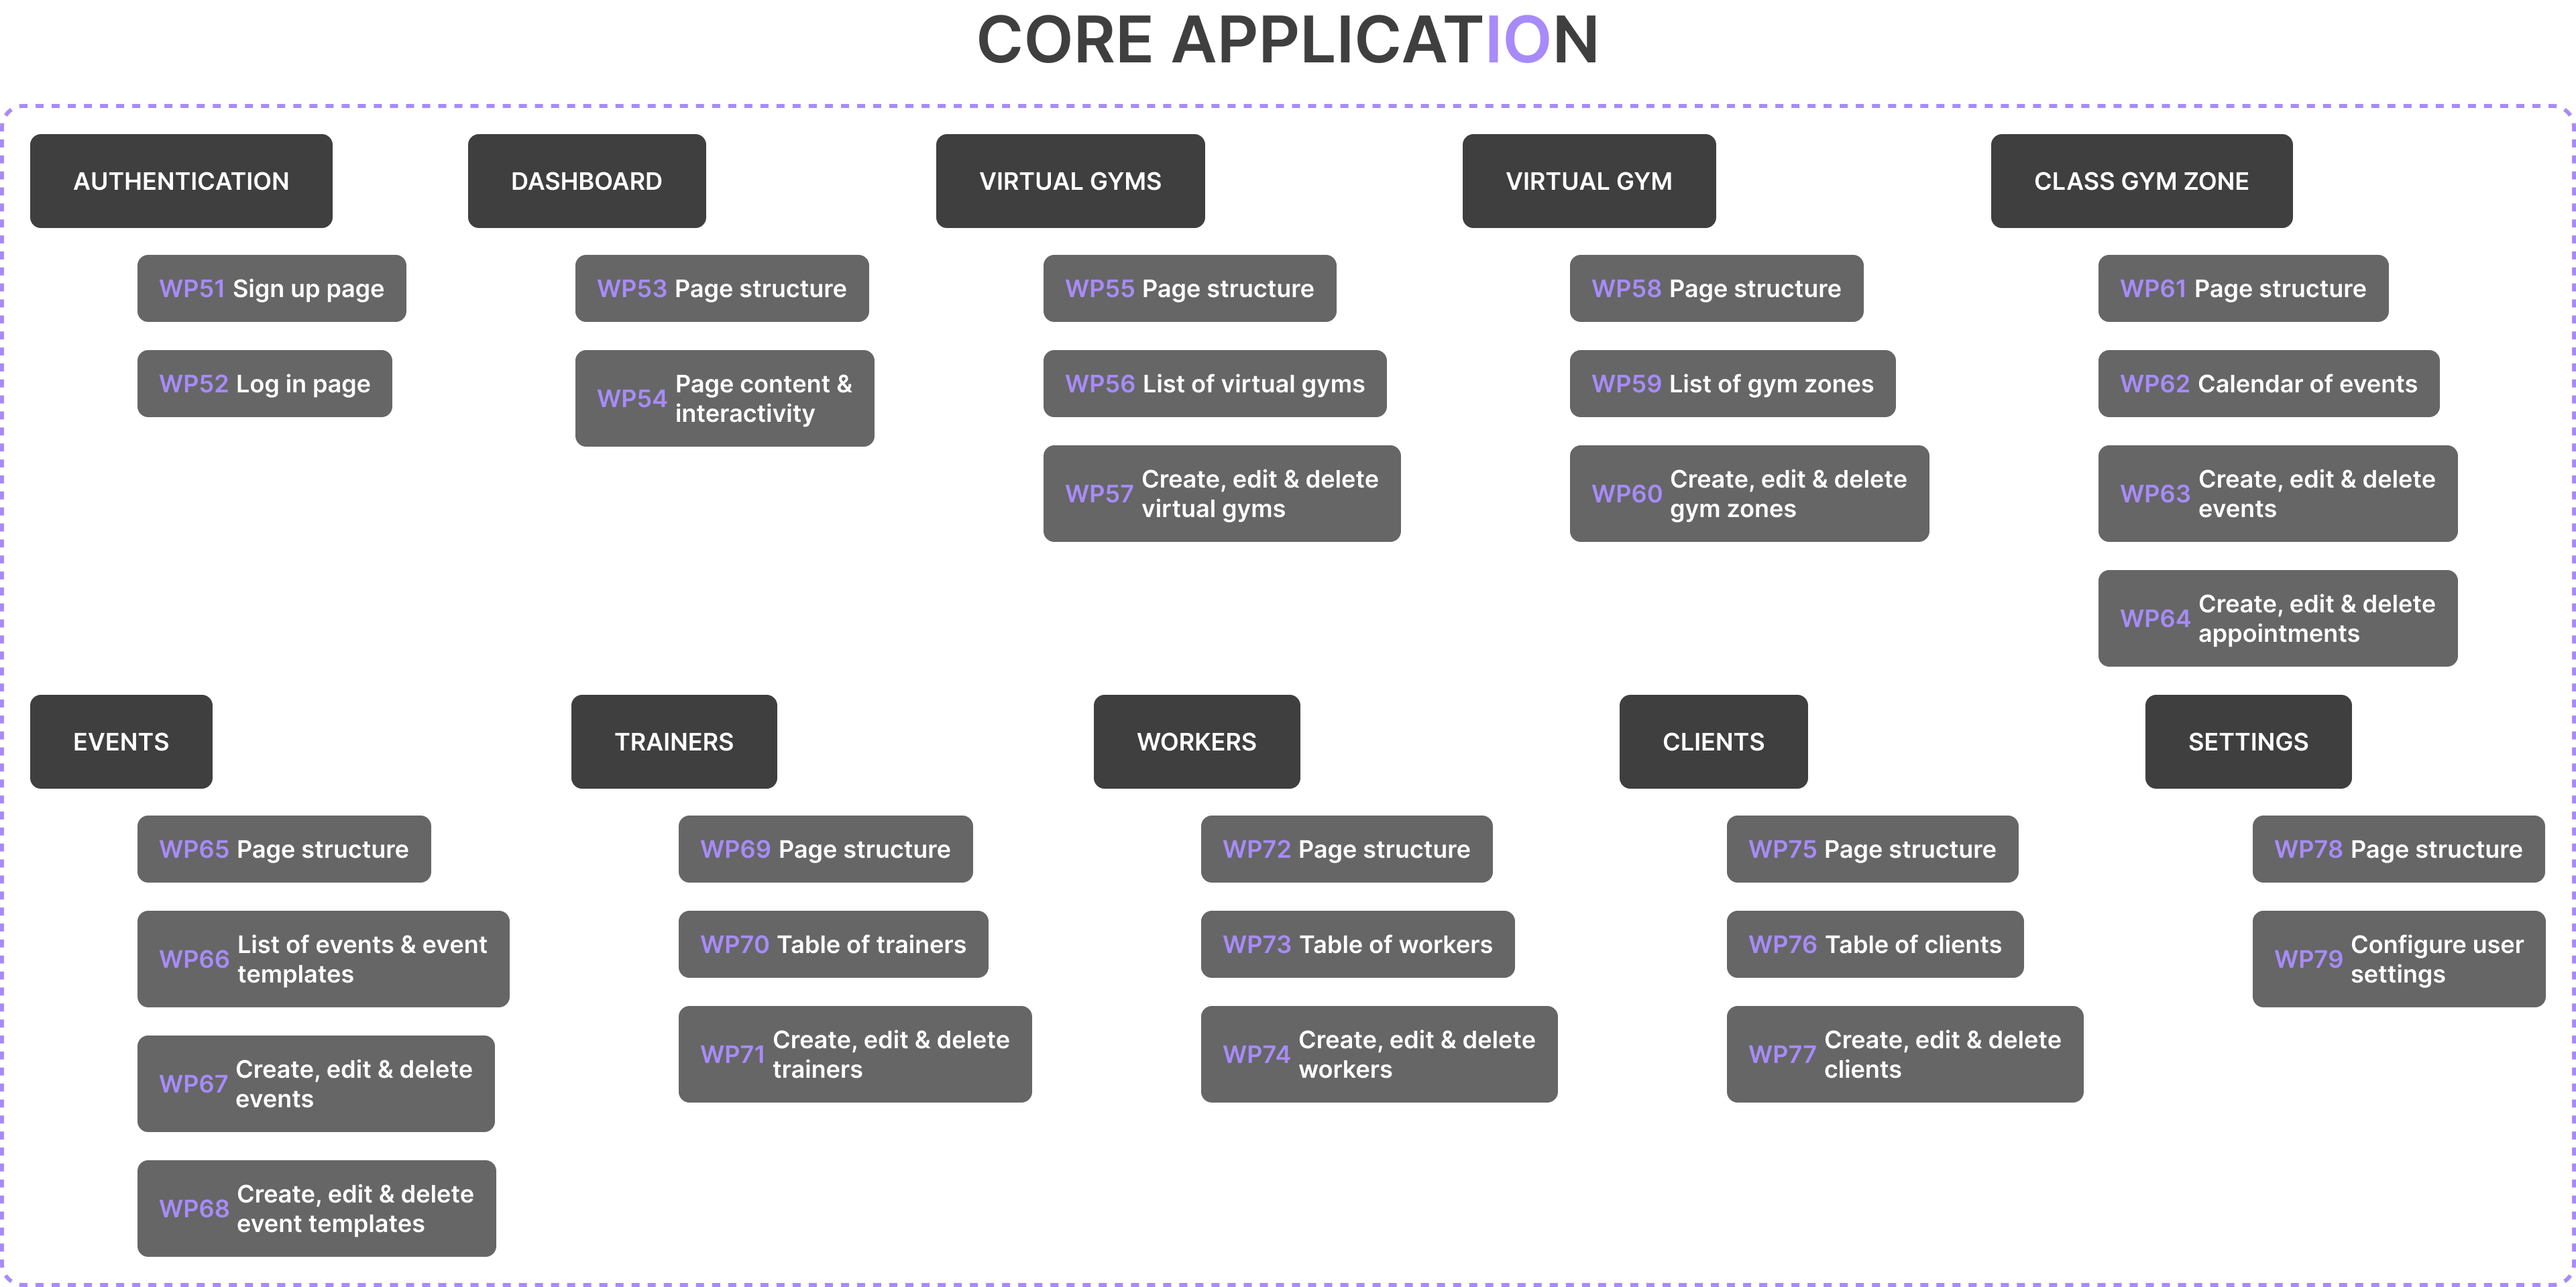
\includegraphics[width=\textwidth]{assets/working-packages/Core.png}
	\caption{Core application working packages diagram}
\end{figure}
The \emph{core} group is composed of the following working packages:
\\[8pt]
\begin{tabularx}{\textwidth}{| l | X |}
	\hline
	\rowcolor{rowColor}
	{\semibf Package name}   & {\semibf WP51}: Sign up page               \\
	\hline
	{\semibf Description}    & Develop the sign up page                   \\
	\hline
	\rowcolor{rowColor}
	{\semibf Estimated time} & 16h                                        \\
	\hline
	{\semibf Tasks}          & {\semibf T1}: Set up the page structure.
	\newline {\semibf T2}: Sign up as an owner.                           \\
	\hline
	\rowcolor{rowColor}
	{\semibf Results}        & Allow the users to register to the system. \\
	\hline
\end{tabularx}
\captionof{table}{Package fifty-one's table - Sign up page}
\vspace*{16pt}
\begin{tabularx}{\textwidth}{| l | X |}
	\hline
	\rowcolor{rowColor}
	{\semibf Package name}   & {\semibf WP52}: Log in page              \\
	\hline
	{\semibf Description}    & Develop the log in page.                 \\
	\hline
	\rowcolor{rowColor}
	{\semibf Estimated time} & 16h                                      \\
	\hline
	{\semibf Tasks}          & {\semibf T1}: Set up the page structure.
	\newline {\semibf T2}: Log in as an owner.
	\newline {\semibf T3}: Log in as a worker.                          \\
	\hline
	\rowcolor{rowColor}
	{\semibf Results}        & Allow the user to log in to the system.  \\
	\hline
\end{tabularx}
\captionof{table}{Package fifty-two's table - Log in page}
\vspace*{16pt}
\begin{tabularx}{\textwidth}{| l | X |}
	\hline
	\rowcolor{rowColor}
	{\semibf Package name}   & {\semibf WP53}: Page structure (Dashboard)            \\
	\hline
	{\semibf Description}    & Apply the design of the dashboard page.               \\
	\hline
	\rowcolor{rowColor}
	{\semibf Estimated time} & 4h                                                    \\
	\hline
	{\semibf Tasks}          & {\semibf T1}: Apply the design of the dashboard page. \\
	\hline
	\rowcolor{rowColor}
	{\semibf Results}        & The scaffolding of the dashboard page.                \\
	\hline
\end{tabularx}
\captionof{table}{Package fifty-three's table - Page structure (Dashboard)}
\vspace*{16pt}
\begin{tabularx}{\textwidth}{| l | X |}
	\hline
	\rowcolor{rowColor}
	{\semibf Package name}   & {\semibf WP54}: Page content and interactivity (Dashboard) \\
	\hline
	{\semibf Description}    & Add the interactivity to the dashboard page.               \\
	\hline
	\rowcolor{rowColor}
	{\semibf Estimated time} & 12h                                                        \\
	\hline
	{\semibf Tasks}          & {\semibf T1}: Add virtual gyms' interactivity.
	\newline {\semibf T2}: Add gym zones' interactivity.
	\newline {\semibf T3}: Add trainers' interactivity.
	\newline {\semibf T4}: Add event templates' interactivity.
	\newline {\semibf T5}: Add events' interactivity.                                     \\
	\hline
	\rowcolor{rowColor}
	{\semibf Results}        & User experience of the dasboard page.                      \\
	\hline
\end{tabularx}
\captionof{table}{Package fifty-four's table - Page content and interactivity}
\vspace*{16pt}
\begin{tabularx}{\textwidth}{| l | X |}
	\hline
	\rowcolor{rowColor}
	{\semibf Package name}   & {\semibf WP55}: Page structure (Virtual gyms)            \\
	\hline
	{\semibf Description}    & Apply the design of the virtual gyms page.               \\
	\hline
	\rowcolor{rowColor}
	{\semibf Estimated time} & 4h                                                       \\
	\hline
	{\semibf Tasks}          & {\semibf T1}: Apply the design of the virtual gyms page. \\
	\hline
	\rowcolor{rowColor}
	{\semibf Results}        & The scaffolding of the virtual gyms page.                \\
	\hline
\end{tabularx}
\captionof{table}{Package fifty-five's table - Page structure (Virtual gyms)}
\vspace*{16pt}
\begin{tabularx}{\textwidth}{| l | X |}
	\hline
	\rowcolor{rowColor}
	{\semibf Package name}   & {\semibf WP56}: List of virtual gyms (Virtual gyms) \\
	\hline
	{\semibf Description}    & Display the list of virtual gyms.                   \\
	\hline
	\rowcolor{rowColor}
	{\semibf Estimated time} & 4h                                                  \\
	\hline
	{\semibf Tasks}          & {\semibf T1}: List the virtual gyms of the gym.
	\newline {\semibf T2}: List the gym zones inside each virtual gym.             \\
	\hline
	\rowcolor{rowColor}
	{\semibf Results}        & The page of virtual gyms.                           \\
	\hline
\end{tabularx}
\captionof{table}{Package fifty-six's table - List of virtual gyms (Virtual gyms)}
\vspace*{16pt}
\begin{tabularx}{\textwidth}{| l | X |}
	\hline
	\rowcolor{rowColor}
	{\semibf Package name}   & {\semibf WP57}: Create, edit and delete virtual gyms (Virtual gyms) \\
	\hline
	{\semibf Description}    & Create the modal to create, edit and delete virtual gyms.           \\
	\hline
	\rowcolor{rowColor}
	{\semibf Estimated time} & 8h                                                                  \\
	\hline
	{\semibf Tasks}          & {\semibf T1}: Modal to create, edit and delete virtual gyms.        \\
	\hline
	\rowcolor{rowColor}
	{\semibf Results}        & The modal to interact with virtual gyms.                            \\
	\hline
\end{tabularx}
\captionof{table}{Package fifty-seven's table - List of virtual gyms (Virtual gyms)}
\vspace*{16pt}
\begin{tabularx}{\textwidth}{| l | X |}
	\hline
	\rowcolor{rowColor}
	{\semibf Package name}   & {\semibf WP58}: Page structure (Virtual gym)            \\
	\hline
	{\semibf Description}    & Apply the design of the virtual gym page.               \\
	\hline
	\rowcolor{rowColor}
	{\semibf Estimated time} & 4h                                                      \\
	\hline
	{\semibf Tasks}          & {\semibf T1}: Apply the design of the virtual gym page. \\
	\hline
	\rowcolor{rowColor}
	{\semibf Results}        & The scaffolding of the virtual gym page.                \\
	\hline
\end{tabularx}
\captionof{table}{Package fitfty-eight's table - Page structure (Virtual gym)}
\vspace*{16pt}
\begin{tabularx}{\textwidth}{| l | X |}
	\hline
	\rowcolor{rowColor}
	{\semibf Package name}   & {\semibf WP59}: List of gym zones (Virtual gym) \\
	\hline
	{\semibf Description}    & List the gym zones of a virtual gym.            \\
	\hline
	\rowcolor{rowColor}
	{\semibf Estimated time} & 8h                                              \\
	\hline
	{\semibf Tasks}          & {\semibf T1}: List all class gym zones.
	\newline {\semibf T2}: List all non-class gym zones.                       \\
	\hline
	\rowcolor{rowColor}
	{\semibf Results}        & The page of a virtual gym.                      \\
	\hline
\end{tabularx}
\captionof{table}{Package fifty-nine's table - List of gym zones (Virtual gym)}
\vspace*{16pt}
\begin{tabularx}{\textwidth}{| l | X |}
	\hline
	\rowcolor{rowColor}
	{\semibf Package name}   & {\semibf WP60}: Create, edit and delete gym zones (Virtual gym) \\
	\hline
	{\semibf Description}    & Create the modal to create, edit and delete gym zones.          \\
	\hline
	\rowcolor{rowColor}
	{\semibf Estimated time} & 8h                                                              \\
	\hline
	{\semibf Tasks}          & {\semibf T1}: Modal to create, edit and delete gym zones.       \\
	\hline
	\rowcolor{rowColor}
	{\semibf Results}        & The modal to interact with gym zones.                           \\
	\hline
\end{tabularx}
\captionof{table}{Package sixty's table - Create, edit and delete gym zones (Virtual gym)}
\vspace*{16pt}
\begin{tabularx}{\textwidth}{| l | X |}
	\hline
	\rowcolor{rowColor}
	{\semibf Package name}   & {\semibf WP61}: Page structure (Class gym zone)            \\
	\hline
	{\semibf Description}    & Apply the design of the class gym zone page.               \\
	\hline
	\rowcolor{rowColor}
	{\semibf Estimated time} & 4h                                                         \\
	\hline
	{\semibf Tasks}          & {\semibf T1}: Apply the design of the class gym zone page. \\
	\hline
	\rowcolor{rowColor}
	{\semibf Results}        & The scaffolding of the class gym zone page.                \\
	\hline
\end{tabularx}
\captionof{table}{Package sixty-one's table - Page structure (Class gym zone)}
\vspace*{16pt}
\begin{tabularx}{\textwidth}{| l | X |}
	\hline
	\rowcolor{rowColor}
	{\semibf Package name}   & {\semibf WP62}: Calendar of events (Class gym zone) \\
	\hline
	{\semibf Description}    & Display the calendar of events of the gym zone.     \\
	\hline
	\rowcolor{rowColor}
	{\semibf Estimated time} & 8h                                                  \\
	\hline
	{\semibf Tasks}          & {\semibf T1}: Design the calendar of events.
	\newline {\semibf T2}: Add interactivity to the calendar.                      \\
	\hline
	\rowcolor{rowColor}
	{\semibf Results}        & The calendar of events for the gym zone.            \\
	\hline
\end{tabularx}
\captionof{table}{Package sixty-two's table - Calendar of events (Class gym zone)}
\vspace*{16pt}
\begin{tabularx}{\textwidth}{| l | X |}
	\hline
	\rowcolor{rowColor}
	{\semibf Package name}   & {\semibf WP63}: Create, edit and delete events (Class gym zone) \\
	\hline
	{\semibf Description}    & Modal to create, edit and delete events.                        \\
	\hline
	\rowcolor{rowColor}
	{\semibf Estimated time} & 8h                                                              \\
	\hline
	{\semibf Tasks}          & {\semibf T1}: Modal to create, edit and delete events.          \\
	\hline
	\rowcolor{rowColor}
	{\semibf Results}        & The modal to interact with events.                              \\
	\hline
\end{tabularx}
\captionof{table}{Package sixty-three's table - Create, edit and delete events (Class gym zone)}
\vspace*{16pt}
\begin{tabularx}{\textwidth}{| l | X |}
	\hline
	\rowcolor{rowColor}
	{\semibf Package name}   & {\semibf WP64}: Create, edit and delete appointments (Class gym zone) \\
	\hline
	{\semibf Description}    & Modal to create, edit and delete appointments.                        \\
	\hline
	\rowcolor{rowColor}
	{\semibf Estimated time} & 8h                                                                    \\
	\hline
	{\semibf Tasks}          & {\semibf T1}: Modal to create, edit and delete appointments.          \\
	\hline
	\rowcolor{rowColor}
	{\semibf Results}        & The modal to interact with appointments.                              \\
	\hline
\end{tabularx}
\captionof{table}{Package sixty-four's table - Create, edit and delete appointments (Class gym zone)}
\vspace*{16pt}
\begin{tabularx}{\textwidth}{| l | X |}
	\hline
	\rowcolor{rowColor}
	{\semibf Package name}   & {\semibf WP65}: Page structure (Events)            \\
	\hline
	{\semibf Description}    & Apply the design of the events page.               \\
	\hline
	\rowcolor{rowColor}
	{\semibf Estimated time} & 4h                                                 \\
	\hline
	{\semibf Tasks}          & {\semibf T1}: Apply the design of the events page. \\
	\hline
	\rowcolor{rowColor}
	{\semibf Results}        & The scaffolding of the events page.                \\
	\hline
\end{tabularx}
\captionof{table}{Package sixty-five's table - Page structure (Events)}
\vspace*{16pt}
\begin{tabularx}{\textwidth}{| l | X |}
	\hline
	\rowcolor{rowColor}
	{\semibf Package name}   & {\semibf WP66}: List of events and event templates (Events) \\
	\hline
	{\semibf Description}    & Display the list of events and event templates.             \\
	\hline
	\rowcolor{rowColor}
	{\semibf Estimated time} & 6h                                                          \\
	\hline
	{\semibf Tasks}          & {\semibf T1}: List the events.
	\newline {\semibf T2}: List the event templates                                        \\
	\hline
	\rowcolor{rowColor}
	{\semibf Results}        & The events page.                                            \\
	\hline
\end{tabularx}
\captionof{table}{Package sixty-six's table - List of events and event tempaltes (Events)}
\vspace*{16pt}
\begin{tabularx}{\textwidth}{| l | X |}
	\hline
	\rowcolor{rowColor}
	{\semibf Package name}   & {\semibf WP67}: Create, edit and delete events (Events) \\
	\hline
	{\semibf Description}    & Modal to create, edit and delete events.                \\
	\hline
	\rowcolor{rowColor}
	{\semibf Estimated time} & 8h                                                      \\
	\hline
	{\semibf Tasks}          & {\semibf T1}: Modal to create, edit and delete events.  \\
	\hline
	\rowcolor{rowColor}
	{\semibf Results}        & The modal to interact with events.                      \\
	\hline
\end{tabularx}
\captionof{table}{Package sixty-seven's table - Create, edit and delete events (Events)}
\vspace*{16pt}
\begin{tabularx}{\textwidth}{| l | X |}
	\hline
	\rowcolor{rowColor}
	{\semibf Package name}   & {\semibf WP68}: Create, edit and delete events templates (Events) \\
	\hline
	{\semibf Description}    & Modal to create, edit and delete events templates.                \\
	\hline
	\rowcolor{rowColor}
	{\semibf Estimated time} & 8h                                                                \\
	\hline
	{\semibf Tasks}          & {\semibf T1}: Modal to create, edit and delete events templates.  \\
	\hline
	\rowcolor{rowColor}
	{\semibf Results}        & The modal to interact with events templates.                      \\
	\hline
\end{tabularx}
\captionof{table}{Package sixty-eight's table - Create, edit and delete events templates (Events)}
\vspace*{16pt}
\begin{tabularx}{\textwidth}{| l | X |}
	\hline
	\rowcolor{rowColor}
	{\semibf Package name}   & {\semibf WP69}: Page structure (Trainers)            \\
	\hline
	{\semibf Description}    & Apply the design of the trainers page.               \\
	\hline
	\rowcolor{rowColor}
	{\semibf Estimated time} & 4h                                                   \\
	\hline
	{\semibf Tasks}          & {\semibf T1}: Apply the design of the trainers page. \\
	\hline
	\rowcolor{rowColor}
	{\semibf Results}        & The scaffolding of the trainers page.                \\
	\hline
\end{tabularx}
\captionof{table}{Package sixty-nine's table - Page structure (Trainers)}
\vspace*{16pt}
\begin{tabularx}{\textwidth}{| l | X |}
	\hline
	\rowcolor{rowColor}
	{\semibf Package name}   & {\semibf WP70}: Table of trainers (Trainers) \\
	\hline
	{\semibf Description}    & Table of trainers.                           \\
	\hline
	\rowcolor{rowColor}
	{\semibf Estimated time} & 4h                                           \\
	\hline
	{\semibf Tasks}          & {\semibf T1}: Display the table of trainers. \\
	\hline
	\rowcolor{rowColor}
	{\semibf Results}        & The table of trainers.                       \\
	\hline
\end{tabularx}
\captionof{table}{Package seventy's table - Table of trainers (Trainers)}
\vspace*{16pt}
\begin{tabularx}{\textwidth}{| l | X |}
	\hline
	\rowcolor{rowColor}
	{\semibf Package name}   & {\semibf WP71}: Create, edit and delete trainers (Trainers) \\
	\hline
	{\semibf Description}    & Modal to create, edit and delete trainers.                  \\
	\hline
	\rowcolor{rowColor}
	{\semibf Estimated time} & 8h                                                          \\
	\hline
	{\semibf Tasks}          & {\semibf T1}: Modal to create, edit and delete trainers.    \\
	\hline
	\rowcolor{rowColor}
	{\semibf Results}        & The modal to interact with trainers.                        \\
	\hline
\end{tabularx}
\captionof{table}{Package seventy-one's table - Table of trainers (Trainers)}
\vspace*{16pt}
\begin{tabularx}{\textwidth}{| l | X |}
	\hline
	\rowcolor{rowColor}
	{\semibf Package name}   & {\semibf WP72}: Page structure (Workers)            \\
	\hline
	{\semibf Description}    & Apply the design of the workers page.               \\
	\hline
	\rowcolor{rowColor}
	{\semibf Estimated time} & 4h                                                  \\
	\hline
	{\semibf Tasks}          & {\semibf T1}: Apply the design of the workers page. \\
	\hline
	\rowcolor{rowColor}
	{\semibf Results}        & The scaffolding of the workers page.                \\
	\hline
\end{tabularx}
\captionof{table}{Package seventy-two's table - Page structure (Workers)}
\vspace*{16pt}
\begin{tabularx}{\textwidth}{| l | X |}
	\hline
	\rowcolor{rowColor}
	{\semibf Package name}   & {\semibf WP73}: Table of workers (Workers)  \\
	\hline
	{\semibf Description}    & Table of workers.                           \\
	\hline
	\rowcolor{rowColor}
	{\semibf Estimated time} & 4h                                          \\
	\hline
	{\semibf Tasks}          & {\semibf T1}: Display the table of workers. \\
	\hline
	\rowcolor{rowColor}
	{\semibf Results}        & The table of workers.                       \\
	\hline
\end{tabularx}
\captionof{table}{Package seventy-three's table - Table of workers (Workers)}
\vspace*{16pt}
\begin{tabularx}{\textwidth}{| l | X |}
	\hline
	\rowcolor{rowColor}
	{\semibf Package name}   & {\semibf WP74}: Create, edit and delete workers (Workers) \\
	\hline
	{\semibf Description}    & Modal to create, edit and delete workers.                 \\
	\hline
	\rowcolor{rowColor}
	{\semibf Estimated time} & 8h                                                        \\
	\hline
	{\semibf Tasks}          & {\semibf T1}: Modal to create, edit and delete workers.   \\
	\hline
	\rowcolor{rowColor}
	{\semibf Results}        & The modal to interact with workers.                       \\
	\hline
\end{tabularx}
\captionof{table}{Package seventy-four's table - Table of workers (Workers)}
\vspace*{16pt}
\begin{tabularx}{\textwidth}{| l | X |}
	\hline
	\rowcolor{rowColor}
	{\semibf Package name}   & {\semibf WP75}: Page structure (Trainers)            \\
	\hline
	{\semibf Description}    & Apply the design of the trainers page.               \\
	\hline
	\rowcolor{rowColor}
	{\semibf Estimated time} & 4h                                                   \\
	\hline
	{\semibf Tasks}          & {\semibf T1}: Apply the design of the trainers page. \\
	\hline
	\rowcolor{rowColor}
	{\semibf Results}        & The scaffolding of the trainers page.                \\
	\hline
\end{tabularx}
\captionof{table}{Package seventy-five's table - Page structure (Trainers)}
\vspace*{16pt}
\begin{tabularx}{\textwidth}{| l | X |}
	\hline
	\rowcolor{rowColor}
	{\semibf Package name}   & {\semibf WP76}: Table of trainers (Trainers) \\
	\hline
	{\semibf Description}    & Table of trainers.                           \\
	\hline
	\rowcolor{rowColor}
	{\semibf Estimated time} & 4h                                           \\
	\hline
	{\semibf Tasks}          & {\semibf T1}: Display the table of trainers. \\
	\hline
	\rowcolor{rowColor}
	{\semibf Results}        & The table of trainers.                       \\
	\hline
\end{tabularx}
\captionof{table}{Package seventy-six's table - Table of trainers (Trainers)}
\vspace*{16pt}
\begin{tabularx}{\textwidth}{| l | X |}
	\hline
	\rowcolor{rowColor}
	{\semibf Package name}   & {\semibf WP77}: Create, edit and delete trainers (Trainers) \\
	\hline
	{\semibf Description}    & Modal to create, edit and delete trainers.                  \\
	\hline
	\rowcolor{rowColor}
	{\semibf Estimated time} & 8h                                                          \\
	\hline
	{\semibf Tasks}          & {\semibf T1}: Modal to create, edit and delete trainers.    \\
	\hline
	\rowcolor{rowColor}
	{\semibf Results}        & The modal to interact with trainers.                        \\
	\hline
\end{tabularx}
\captionof{table}{Package seventy-seven's table - Table of trainers (Trainers)}
\vspace*{16pt}
\begin{tabularx}{\textwidth}{| l | X |}
	\hline
	\rowcolor{rowColor}
	{\semibf Package name}   & {\semibf WP78}: Page structure (Settings)            \\
	\hline
	{\semibf Description}    & Apply the design of the settings page.               \\
	\hline
	\rowcolor{rowColor}
	{\semibf Estimated time} & 4h                                                   \\
	\hline
	{\semibf Tasks}          & {\semibf T1}: Apply the design of the settings page. \\
	\hline
	\rowcolor{rowColor}
	{\semibf Results}        & The scaffolding of the settings page.                \\
	\hline
\end{tabularx}
\captionof{table}{Package seventy-eight's table - Page structure (Settings)}
\vspace*{16pt}
\begin{tabularx}{\textwidth}{| l | X |}
	\hline
	\rowcolor{rowColor}
	{\semibf Package name}   & {\semibf WP79}: Configure user settings (Settings) \\
	\hline
	{\semibf Description}    & Set up the form to update user settings.           \\
	\hline
	\rowcolor{rowColor}
	{\semibf Estimated time} & 8h                                                 \\
	\hline
	{\semibf Tasks}          & {\semibf T1}: Log out the user.
	\newline {\semibf T2}: Configure the basic fields of the user.
	\newline {\semibf T3}: Update the user password.
	\newline {\semibf T4}: Update the gym information as an owner.                \\
	\hline
	\rowcolor{rowColor}
	{\semibf Results}        & The settings page.                                 \\
	\hline
\end{tabularx}
\captionof{table}{Package seventy-nine's table - Configure user settings (Settings)}
\vspace*{16pt}
\subsubsection{Client application}
The \emph{landing} group of working packages follows a similar approach as the one described in \emph{\nameref{working-packages-development}}.
\begin{figure}[H]
	\centering
	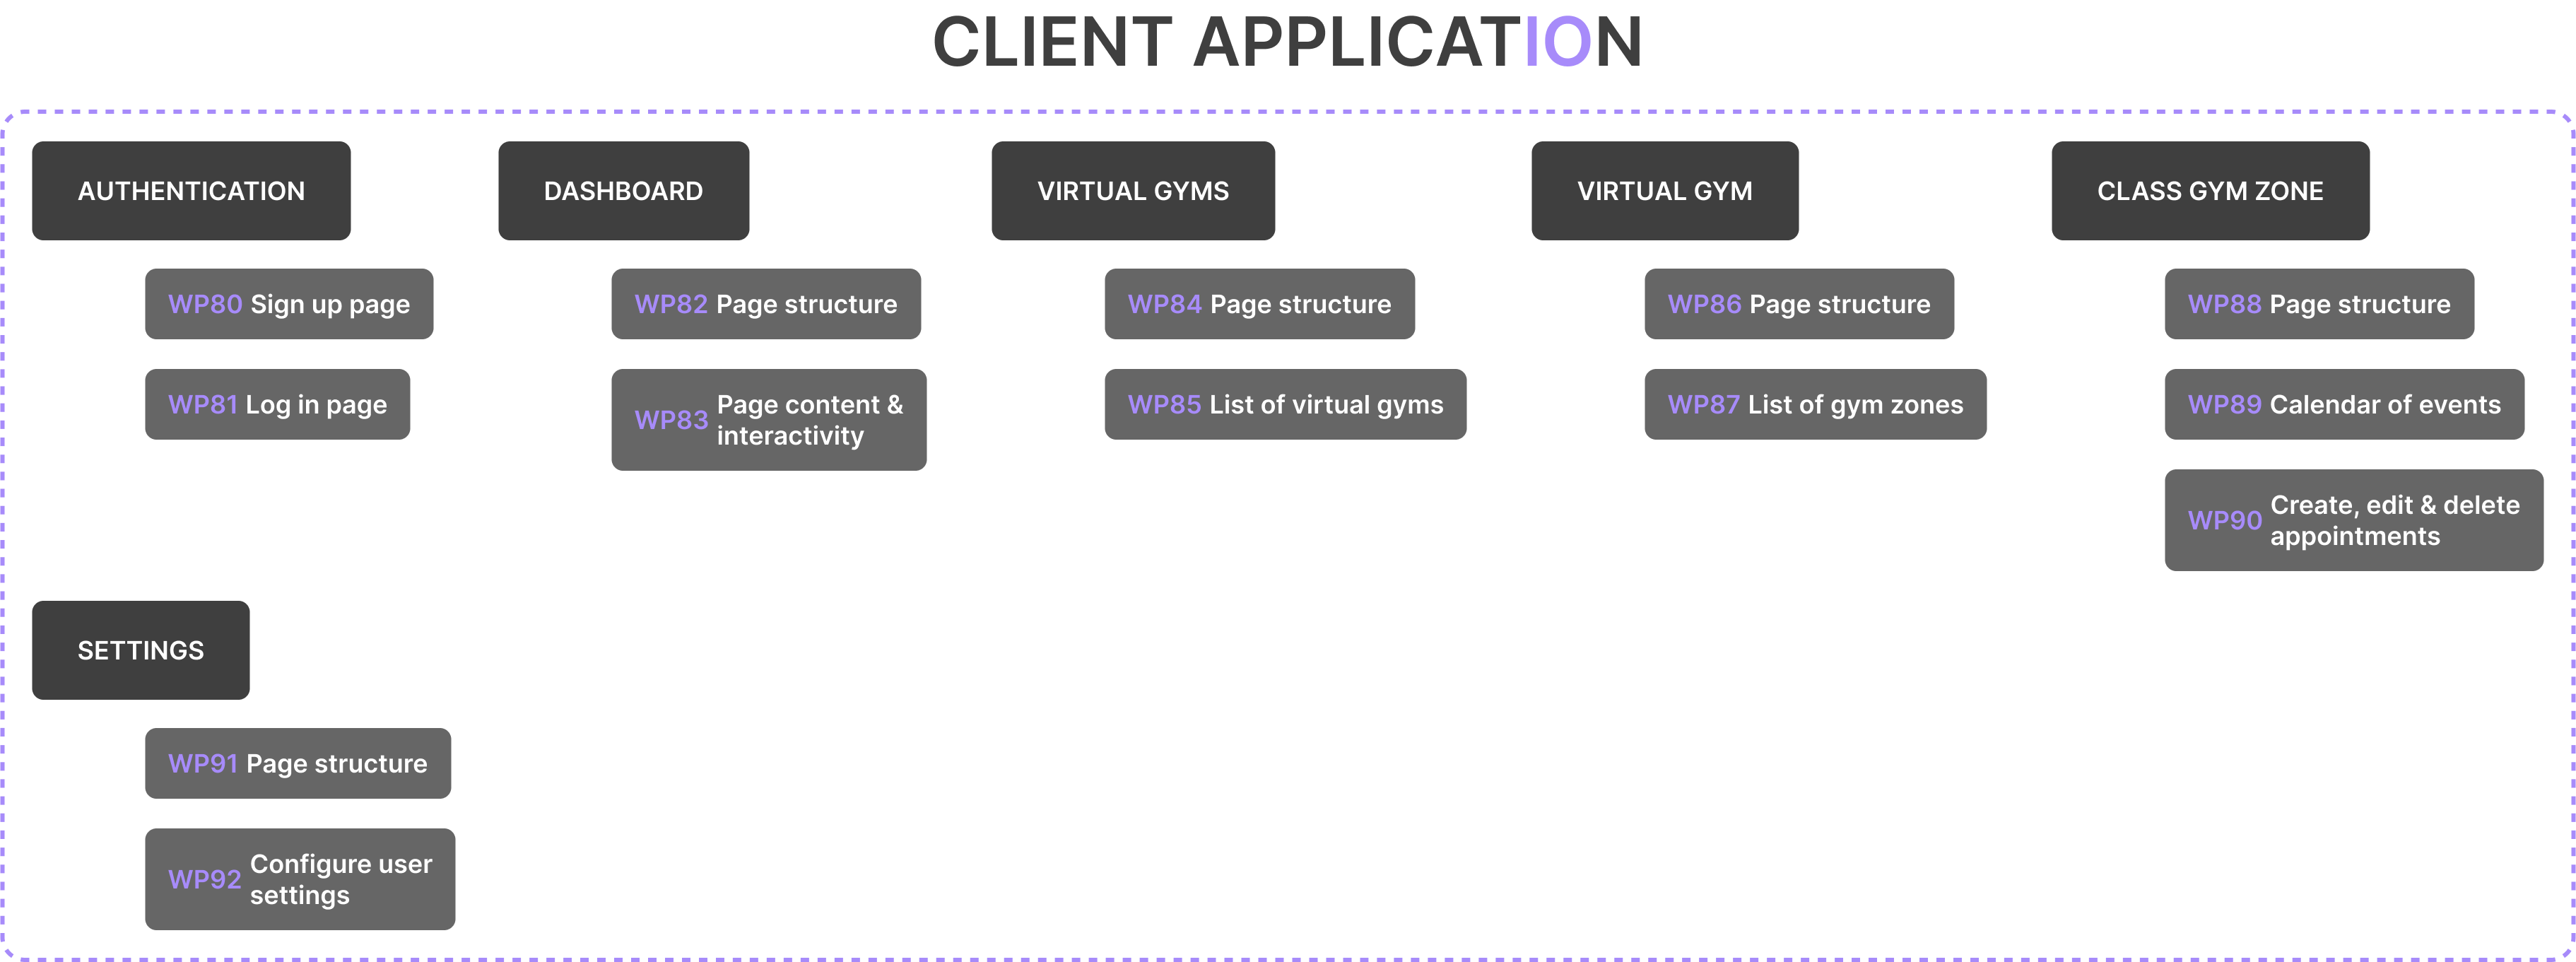
\includegraphics[width=\textwidth]{assets/working-packages/Client.png}
	\caption{Client application working packages diagram}
\end{figure}
The \emph{client} group is composed of the following working packages:
\\[8pt]
\begin{tabularx}{\textwidth}{| l | X |}
	\hline
	\rowcolor{rowColor}
	{\semibf Package name}   & {\semibf WP80}: Sign up page                 \\
	\hline
	{\semibf Description}    & Develop the sign up page                     \\
	\hline
	\rowcolor{rowColor}
	{\semibf Estimated time} & 8h                                           \\
	\hline
	{\semibf Tasks}          & {\semibf T1}: Set up the page structure.
	\newline {\semibf T2}: Sign up as a client.                             \\
	\hline
	\rowcolor{rowColor}
	{\semibf Results}        & Allow the clients to register to the system. \\
	\hline
\end{tabularx}
\captionof{table}{Package eighty's table - Sign up page}
\vspace*{16pt}
\begin{tabularx}{\textwidth}{| l | X |}
	\hline
	\rowcolor{rowColor}
	{\semibf Package name}   & {\semibf WP81}: Log in page              \\
	\hline
	{\semibf Description}    & Develop the log in page.                 \\
	\hline
	\rowcolor{rowColor}
	{\semibf Estimated time} & 8h                                       \\
	\hline
	{\semibf Tasks}          & {\semibf T1}: Set up the page structure.
	\newline {\semibf T2}: Log in as a client.                          \\
	\hline
	\rowcolor{rowColor}
	{\semibf Results}        & Allow the user to log in to the system.  \\
	\hline
\end{tabularx}
\captionof{table}{Package eighty-one's table - Log in page}
\vspace*{16pt}
\begin{tabularx}{\textwidth}{| l | X |}
	\hline
	\rowcolor{rowColor}
	{\semibf Package name}   & {\semibf WP82}: Page structure (Dashboard)            \\
	\hline
	{\semibf Description}    & Apply the design of the dashboard page.               \\
	\hline
	\rowcolor{rowColor}
	{\semibf Estimated time} & 4h                                                    \\
	\hline
	{\semibf Tasks}          & {\semibf T1}: Apply the design of the dashboard page. \\
	\hline
	\rowcolor{rowColor}
	{\semibf Results}        & The scaffolding of the dashboard page.                \\
	\hline
\end{tabularx}
\captionof{table}{Package eighty-two's table - Page structure (Dashboard)}
\vspace*{16pt}
\begin{tabularx}{\textwidth}{| l | X |}
	\hline
	\rowcolor{rowColor}
	{\semibf Package name}   & {\semibf WP83}: Page content and interactivity (Dashboard) \\
	\hline
	{\semibf Description}    & Add the interactivity to the dashboard page.               \\
	\hline
	\rowcolor{rowColor}
	{\semibf Estimated time} & 6h                                                         \\
	\hline
	{\semibf Tasks}          & {\semibf T1}: Add virtual gyms' interactivity.
	\newline {\semibf T2}: Add gym zones' interactivity.                                  \\
	\hline
	\rowcolor{rowColor}
	{\semibf Results}        & User experience of the dasboard page.                      \\
	\hline
\end{tabularx}
\captionof{table}{Package eighty-three's table - Page content and interactivity}
\vspace*{16pt}
\begin{tabularx}{\textwidth}{| l | X |}
	\hline
	\rowcolor{rowColor}
	{\semibf Package name}   & {\semibf WP84}: Page structure (Virtual gyms)                            \\
	\hline
	{\semibf Description}    & Apply the design of the virtual gyms page. Should reuse the core's page. \\
	\hline
	\rowcolor{rowColor}
	{\semibf Estimated time} & 4h                                                                       \\
	\hline
	{\semibf Tasks}          & {\semibf T1}: Apply the design of the virtual gyms page.                 \\
	\hline
	\rowcolor{rowColor}
	{\semibf Results}        & The scaffolding of the virtual gyms page.                                \\
	\hline
\end{tabularx}
\captionof{table}{Package eighty-fourt's table - Page structure (Virtual gyms)}
\vspace*{16pt}
\begin{tabularx}{\textwidth}{| l | X |}
	\hline
	\rowcolor{rowColor}
	{\semibf Package name}   & {\semibf WP85}: List of virtual gyms (Virtual gyms) \\
	\hline
	{\semibf Description}    & Display the list of virtual gyms.                   \\
	\hline
	\rowcolor{rowColor}
	{\semibf Estimated time} & 4h                                                  \\
	\hline
	{\semibf Tasks}          & {\semibf T1}: List the virtual gyms of the gym.
	\newline {\semibf T2}: List the gym zones inside each virtual gym.             \\
	\hline
	\rowcolor{rowColor}
	{\semibf Results}        & The page of virtual gyms.                           \\
	\hline
\end{tabularx}
\captionof{table}{Package eighty-five's table - List of virtual gyms (Virtual gyms)}
\vspace*{16pt}
\begin{tabularx}{\textwidth}{| l | X |}
	\hline
	\rowcolor{rowColor}
	{\semibf Package name}   & {\semibf WP86}: Page structure (Virtual gym)                            \\
	\hline
	{\semibf Description}    & Apply the design of the virtual gym page. Should reuse the core's page. \\
	\hline
	\rowcolor{rowColor}
	{\semibf Estimated time} & 4h                                                                      \\
	\hline
	{\semibf Tasks}          & {\semibf T1}: Apply the design of the virtual gym page.                 \\
	\hline
	\rowcolor{rowColor}
	{\semibf Results}        & The scaffolding of the virtual gym page.                                \\
	\hline
\end{tabularx}
\captionof{table}{Package eighty-six's table - Page structure (Virtual gym)}
\vspace*{16pt}
\begin{tabularx}{\textwidth}{| l | X |}
	\hline
	\rowcolor{rowColor}
	{\semibf Package name}   & {\semibf WP87}: List of gym zones (Virtual gym) \\
	\hline
	{\semibf Description}    & List the gym zones of a virtual gym.            \\
	\hline
	\rowcolor{rowColor}
	{\semibf Estimated time} & 4h                                              \\
	\hline
	{\semibf Tasks}          & {\semibf T1}: List all class gym zones.
	\newline {\semibf T2}: List all non-class gym zones.                       \\
	\hline
	\rowcolor{rowColor}
	{\semibf Results}        & The page of a virtual gym.                      \\
	\hline
\end{tabularx}
\captionof{table}{Package eighty-seven's table - List of gym zones (Virtual gym)}
\vspace*{16pt}
\begin{tabularx}{\textwidth}{| l | X |}
	\hline
	\rowcolor{rowColor}
	{\semibf Package name}   & {\semibf WP88}: Page structure (Class gym zone)                            \\
	\hline
	{\semibf Description}    & Apply the design of the class gym zone page. Should reuse the core's page. \\
	\hline
	\rowcolor{rowColor}
	{\semibf Estimated time} & 4h                                                                         \\
	\hline
	{\semibf Tasks}          & {\semibf T1}: Apply the design of the class gym zone page.                 \\
	\hline
	\rowcolor{rowColor}
	{\semibf Results}        & The scaffolding of the class gym zone page.                                \\
	\hline
\end{tabularx}
\captionof{table}{Package eighty-eight's table - Page structure (Class gym zone)}
\vspace*{16pt}
\begin{tabularx}{\textwidth}{| l | X |}
	\hline
	\rowcolor{rowColor}
	{\semibf Package name}   & {\semibf WP89}: Calendar of events (Class gym zone) \\
	\hline
	{\semibf Description}    & Display the calendar of events of the gym zone.     \\
	\hline
	\rowcolor{rowColor}
	{\semibf Estimated time} & 4h                                                  \\
	\hline
	{\semibf Tasks}          & {\semibf T1}: Design the calendar of events.
	\newline{\semibf T2}: Add interactivity to the calendar.                       \\
	\hline
	\rowcolor{rowColor}
	{\semibf Results}        & The calendar of events for the gym zone.            \\
	\hline
\end{tabularx}
\captionof{table}{Package ninety's table - Calendar of events (Class gym zone)}
\vspace*{16pt}
\begin{tabularx}{\textwidth}{| l | X |}
	\hline
	\rowcolor{rowColor}
	{\semibf Package name}   & {\semibf WP90}: Create, edit and delete appointments (Class gym zone) \\
	\hline
	{\semibf Description}    & Modal to create, edit and delete appointments.                        \\
	\hline
	\rowcolor{rowColor}
	{\semibf Estimated time} & 8h                                                                    \\
	\hline
	{\semibf Tasks}          & {\semibf T1}: Modal to create, edit and delete appointments.          \\
	\hline
	\rowcolor{rowColor}
	{\semibf Results}        & The modal to interact with appointments.                              \\
	\hline
\end{tabularx}
\captionof{table}{Package ninety's table - Create, edit and delete appointments (Class gym zone)}
\vspace*{16pt}
\begin{tabularx}{\textwidth}{| l | X |}
	\hline
	\rowcolor{rowColor}
	{\semibf Package name}   & {\semibf WP91}: Page structure (Settings)                            \\
	\hline
	{\semibf Description}    & Apply the design of the settings page. Should reuse the core's page. \\
	\hline
	\rowcolor{rowColor}
	{\semibf Estimated time} & 4h                                                                   \\
	\hline
	{\semibf Tasks}          & {\semibf T1}: Apply the design of the settings page.                 \\
	\hline
	\rowcolor{rowColor}
	{\semibf Results}        & The scaffolding of the settings page.                                \\
	\hline
\end{tabularx}
\captionof{table}{Package ninety-one's table - Page structure (Settings)}
\vspace*{16pt}
\begin{tabularx}{\textwidth}{| l | X |}
	\hline
	\rowcolor{rowColor}
	{\semibf Package name}   & {\semibf WP92}: Configure user settings (Settings) \\
	\hline
	{\semibf Description}    & Set up the form to update client settings.         \\
	\hline
	\rowcolor{rowColor}
	{\semibf Estimated time} & 4h                                                 \\
	\hline
	{\semibf Tasks}          & {\semibf T1}: Log out the client.
	\newline {\semibf T2}: Configure the basic fields of the client.
	\newline {\semibf T3}: Update the client password.                            \\
	\hline
	\rowcolor{rowColor}
	{\semibf Results}        & The settings page.                                 \\
	\hline
\end{tabularx}
\captionof{table}{Package ninety-two's table - Configure user settings (Settings)}
\subsubsection{Landing application}
The landing application is a simple application that displays information about the system and acces to the main application.
\\
\begin{tabularx}{\textwidth}{| l | X |}
	\hline
	\rowcolor{rowColor}
	{\semibf Package name}   & {\semibf WP93}: Design the landing application            \\
	\hline
	{\semibf Description}    & Set up the form to update client settings.                \\
	\hline
	\rowcolor{rowColor}
	{\semibf Estimated time} & 16h                                                       \\
	\hline
	{\semibf Tasks}          & {\semibf T1}: Display basic information about the system.
	\newline {\semibf T2}: Display information about the data privacy.
	\newline {\semibf T3}: Display a contact form.                                       \\
	\hline
	\rowcolor{rowColor}
	{\semibf Results}        & The landing application.                                  \\
	\hline
\end{tabularx}
\captionof{table}{Package ninety-three's table - Landing page}
% endregion PLANNING_TABLES
\section{Traceability matrix}
Due to the large quantity of requirements and working packageds that have been determined for the development of the project, and due to the low relationship between them, the traceability matrix will be shown individually, in order to avoid displaying a nearly empty table. Using the following notation, the result is more consise and can be understood better.
\\[8pt]
Each dependency will use the following format: \textbf{[FR-1] \texttt{->} [WP-1, WP-2, WP-3]}. It states that the functional requirements 1 will be covered in the working package 1, 2 and 3.
\begin{enumerate}[label = -]
	\item \textbf{[FR-1, FR-2, FR-3, FR-4] \texttt{->} [WP-93]}
	\item \textbf{[FR-5, FR-6] \texttt{->} [WP-51]}
	\item \textbf{[FR-7] \texttt{->} [WP-52]}
	\item \textbf{[FR-8, FR-9, FR-10] \texttt{->} [WP-93]}
	\item \textbf{[FR-11, FR-13, FR-14, FR-15, FR-17] \texttt{->} [WP-56, WP-28, WP-29, WP-30]}
	\item \textbf{[FR-12, FR-16] \texttt{->} [WP-57, WP-27, WP-28, WP-29]}
	\item \textbf{[FR-19, FR-21, FR-22] \texttt{->} [WP-59, WP-34]}
	\item \textbf{[FR-20, FR-23] \texttt{->} [WP-60, WP-31, WP-32, WP-33]}
	\item \textbf{[FR-24, FR-27, FR-28] \texttt{->} [WP-62, WP-43, WP-44, WP-45, WP-47, WP-48, WP-49]}
	\item \textbf{[FR-25, FR-26, FR-29, FR-30] \texttt{->} [WP-63, WP-34, WP-46, WP-50]}
	\item \textbf{[FR-31, FR-33] \texttt{->} [WP-66, WP-38, WP-42, WP-46]}
	\item \textbf{[FR-32, FR-35] \texttt{->} [WP-67, WP-35, WP-36, WP-37]}
	\item \textbf{[FR-34, FR-36] \texttt{->} [WP-68, WP-39, WP-40, WP-41]}
	\item \textbf{[FR-37, FR-38, FR-40] \texttt{->} [WP-74, WP-19, WP-20, WP-21]}
	\item \textbf{[FR-39, FR-41] \texttt{->} [WP-73, WP-22]}
	\item \textbf{[FR-42, FR-43, FR-45] \texttt{->} [WP-70, WP-23, WP-24, WP-25]}
	\item \textbf{[FR-44, FR-46] \texttt{->} [WP-71, WP-26]}
	\item \textbf{[FR-47, FR-48] \texttt{->} [WP-77]}
	\item \textbf{[FR-49, FR-50] \texttt{->} [WP-76]}
	\item \textbf{[FR-51, FR-52, FR-53, FR-54, FR-55, FR-56] \texttt{->} [WP-79, WP-17]}
	\item \textbf{[FR-65] \texttt{->} [WP-80, WP-16]}
	\item \textbf{[FR-66] \texttt{->} [WP-81, WP-17]}
	\item \textbf{[FR-67, FR-68] \texttt{->} [WP-85, WP-30]}
	\item \textbf{[FR-69] \texttt{->} [WP-89, WP-46]}
	\item \textbf{[FR-70, FR-71, FR-72] \texttt{->} [WP-90, WP-43, WP-44, WP-45, WP-47, WP-48, WP-49]}
	\item \textbf{[FR-73, FR-74, FR-75, FR-76, FR-77, FR-78] \texttt{->} [WP-92, WP-17]}
	\item \textbf{[NFR-1] \texttt{->} [WP-16, WP-18]}
	\item \textbf{[NFR-2] \texttt{->} [WP-52]}
	\item \textbf{[NFR-3] \texttt{->} [WP-93]}
	\item \textbf{[NFR-4] \texttt{->} [WP-53, WP-55, WP-58, WP-61, WP-65, WP-69, WP-72, WP-75, WP-78]}
	\item \textbf{[NFR-5] \texttt{->} [WP-53, WP-55, WP-58, WP-61, WP-65, WP-69, WP-72, WP-75, WP-78, WP-82, WP-84, WP-86, WP-88, WP-91, WP-93]}
\end{enumerate}
\section{Roadmap}
The roadmap contains an estimation of how the development of the application should. Nonetheless, it is just an estimation and many things may occur that could change such schedule. The projec that is expected to take up most of the amount of tiume is the \emph{core} app, as it is the onw that contains the most amount of logic, followed by the server. Even though the projects are structured sequentially, bugs or errors may occur while developing, for instance, a web service does not return what it should\footnote{The applications will be tested, yet tests do not ensure a 100\% correctness of the application. If the test does not contemplate all corner-cases, there may be a bug.}, which would imply to have it fixed while another app is being developed.
\newpage
\begin{figure}[H]
	\centering
	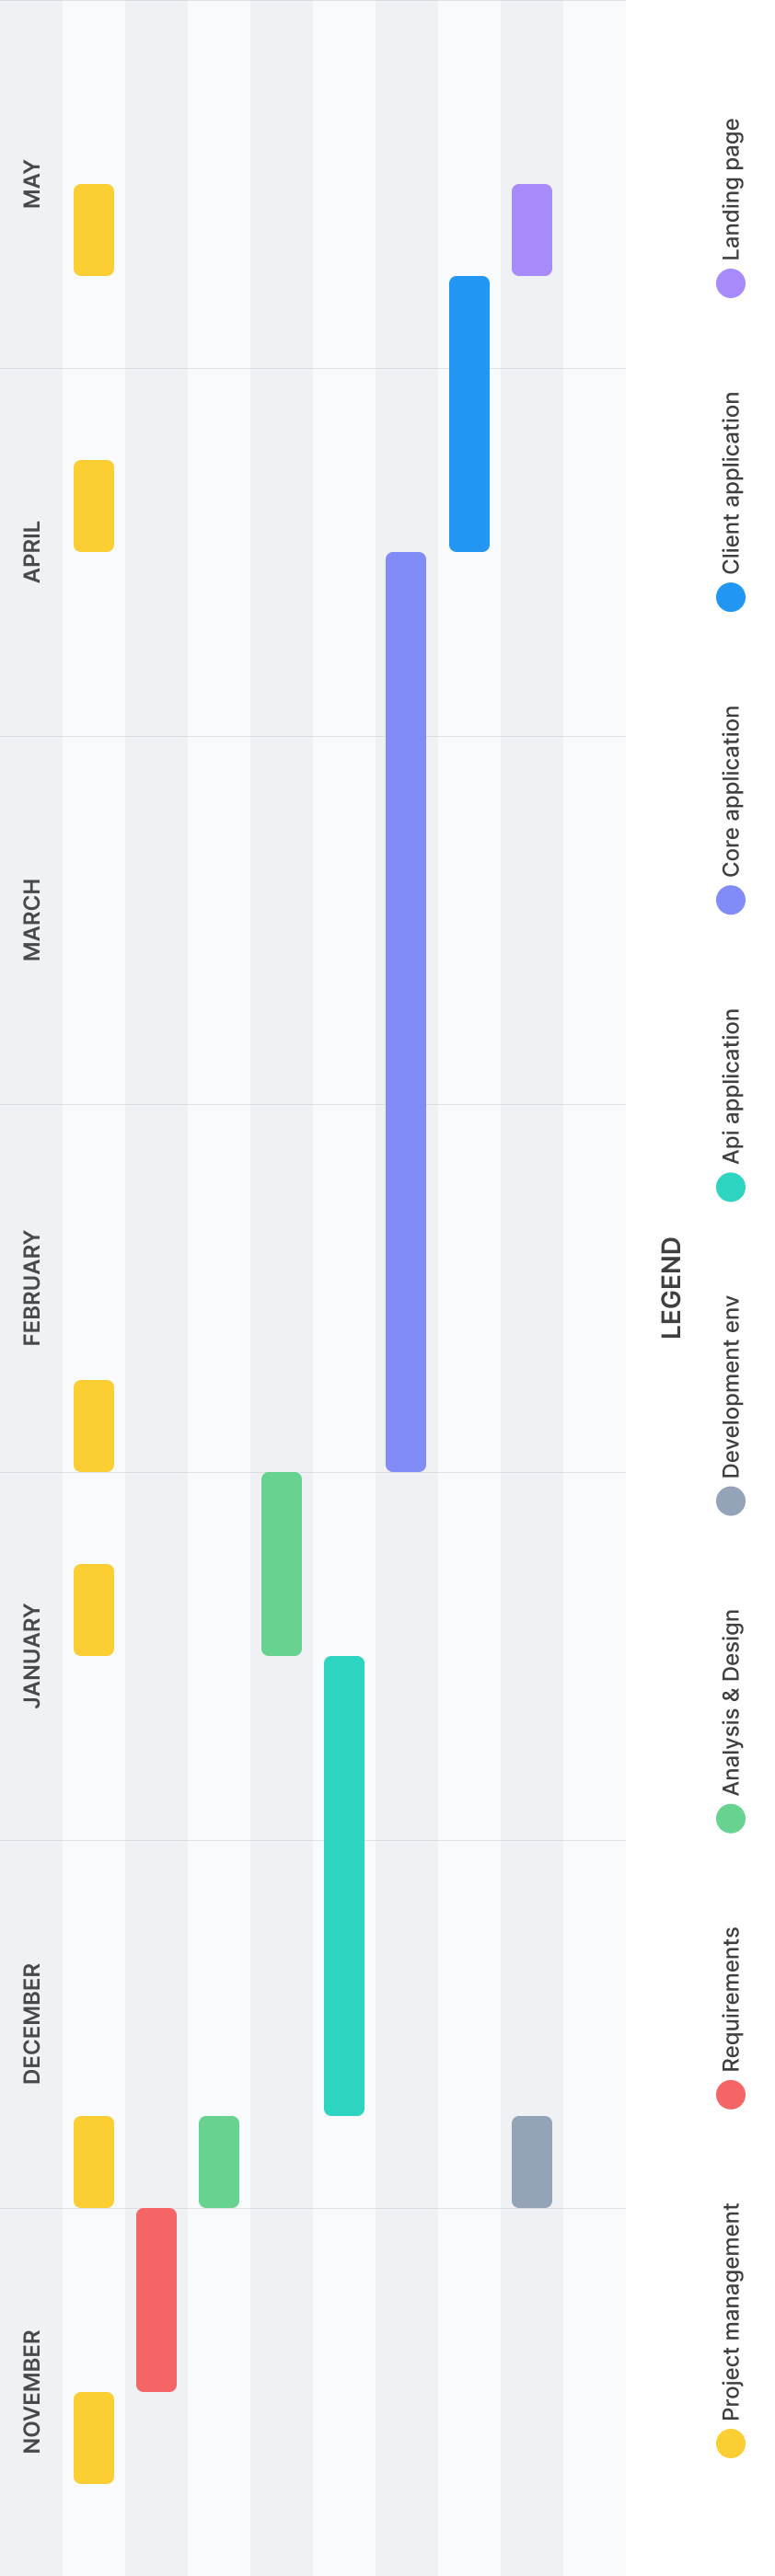
\includegraphics[width=0.45\textwidth]{assets/roadmap.png}
	\caption{Expected application development roadmap.}
\end{figure}
\chapter{Studies and decisions}
\section{Introduction}
This chapter will cover the different aspects that have been taken into account in order to choose the technology stack used to develop the system.
\section{Project structure}
Being able to solve problems rapidly, or even minimizing such errors, it is a must in order to provide a secure and stable application. Since \emph{test driven development} (or \emph{behavior driven development}) was designed, more and bigger companies started incorporating such approach when developing new projects. Nowadays, testing the code that is being developed is unquestionable.
\\[8pt]
Aside from the development method used, it is indisputable to use a version control system. The VCS that takes the gold medal is \emph{git} which is used alongside \emph{GitHub}. From there, the applications can be structured in two forms:
\begin{enumerate}[label = -]
	\item \emph{Multirepo}. The multirepo approach means to have multiple applications in different repositories. The main benefits of such approach are the fact that teams can separately work in the repository while at the same time the repository is kept smaller and cleaner.
	\item \emph{Monorepo}. The monorepo approach is the opposite of the multirepo: all the applications are kept in the same repository. Such approach allows maintaining build and deployment patterns altogether. However, application versioning may be harder.
\end{enumerate}
Since all the applications are build using the same language (\emph{TypeScript}) and the same package manager (\emph{npm}), the monorepo approach has been used.
\subsection{TDD and CI}
The test driven development approach has been the method to ensure that what was being written would do as expected, even when new features are added. Both client and server applications include unit and end-to-end (\emph{e2e}) tests.
\\[8pt]
Unit tests allow the developer to test a feature by isolating all its dependencies. For instance, each method of a concrete service from the backend has it own unit tests which completely mock its dependencies and ensure the behaviour is as expected. On the other hand, the e2e contexts are more complex, since they test, for example, one of the different use cases. An example would be to simulate the behaviour of the user in a client app and expect the DOM to properly change.
\\[8pt]
With testing, comes continuous integration which allows the code to be constantly tested. By constantly checking the newly added code, future errors can be prevented and \emph{post-deployment} breaks or bugs can be reduced. The chosen continuous integration platform is \emph{GitHub Actions}\footnote{The \emph{workflow} files of the platform can be found in the \texttt{.github/workflows} folder of the repository.}
\subsection{Nx}
There exist many systems or libraries that allow the development team to maintain a healthy and scalable monorepo (examples are \emph{Bazel} or \emph{Pants}). In this system, since the language is the same for both web and server applications, the monorepo build framework used that has been chosen is \emph{Nx}. As stated in their repository: \emph{Nx is a smart and extensible build framework to help you architect, test, and build at any scale}.
\begin{figure}[H]
	\centering
	
\includegraphics[width=0.2\textwidth]{assets/nx-logo.png}
	\caption{Nx logo}
\end{figure}
Using such tool, managing the applications becomes extremely easy to manage both JavaScript and TypeScript monorepos. Other key features are:
\begin{enumerate}[label = -]
	\item The different applications have been \emph{generated} using the plugins also developed and maintained by the team behind Nx.
	\item The fast creation of shared libraries.
	\item Testing and building only the affected code. Therefore, in unit testing only the files that have been changed, reduces the amount of tests to be done on each push.
	\item All the created libraries and applications include all the dependencies, scripts and tools to fast serve, test, build and deploy. Additionally, it can \emph{lint} and format the projects.
	\item Provides a rich plugin ecosystem if some utilities are not included in the core package.
\end{enumerate}
More specifically, it has great support with \emph{NextJS}, which is the front-end framework used for the web apps. Being able to easily scale, maintain and test the front-end applications is a crucial requisite in this system. Such tool and its excellent documentation have simplified all aspects for setting up the different apps.
\\[8pt]
After using Nx, the application folder structure is as follows:
\begin{verbatim}
hubbl
├── apps
│   ├── api
│   ├── client
│   ├── client-e2e
│   ├── core
│   ├── core-e2e
│   ├── landing
│   └── landing-e2e
├── libs
│   ├── data-access
│   │   ├── api
│   │   └── contexts
│   ├── shared
│   │   ├── models
│   │   └── types
│   ├── ui
│   │   └── components
│   └── utils
│       └── src
└── tools
    └── generators
        └── component
\end{verbatim}
There are other files in the root folder of the repository, yet they have been excluded as the main folders are \texttt{apps} and \texttt{libs}. On the one hand, the \texttt{apps} folder contains the source code and additional files to build and compile each one of them. The client apps have two folders: the source code folders (\texttt{core}, \texttt{landing} and \texttt{client}) and their respective e2e test folders (\texttt{core-e2e}, \texttt{landing-e2e} and \texttt{client-e2e}). On the other hand, the folder \texttt{libs} contains all the libraries which do not belong to an application, but rather used in many of them. As the Nx documentation states, the \texttt{libs} folder should contain: \emph{Libs contain services, components, utilities, etc. They have well-defined public API.} The front-end applications have been generated using the \texttt{@nrwl/next} utility, while the back end has been generated with \texttt{@nrwl/express}. The libraries have been created with the \texttt{@nx/workspace} which provides a lot of utils for the overall workspace \cite{nx}. Finally, Nx provides an utilities' library that can help the team with common tasks. Such tools are kept in the \texttt{tools} folder. In this case, there is only one tool, \texttt{component}, whih is a generator that when run generates the basic component structured used in \texttt{libs/ui/components}.
\section{Technology stack}
This section will cover the different technologies that are specifically used to develop the different applications.
\subsection{TypeScript}
These days JavaScript is the most used language around the world for many reasons. Nevertheless, due to the fact of not having types, it makes some applications harder to debug and more error-prone. That is one of the reasons why Microsoft developed TypeScript, which is a strict syntactical superset of JavaScript. The code written in TypeScript is transcompiled to JavaScript at build time.
\begin{figure}[H]
	\centering
	
\includegraphics[width=0.175\textwidth]{assets/js-logo.png}
	
\includegraphics[width=0.175\textwidth]{assets/ts-logo.png}
	\caption{JavaScript and TypeScript logos}
\end{figure}
By using TypeScript we provide a highly productive environment when developing the different apps. Not only reduces the amount of painful bugs due to type errors, but also provides all the benefits of the ECMA script.
\subsection{Front end - Web applications}
Nowadays, there are many JavaScript front-end frameworks all with their benefits and disadvantages. Angular, React, Vue and Svelte are the most known and used frameworks. Since I am most experienced with React and NextJS is built upon React, it has been the chosen option. Furthermore, on October 21st of 2021, the NextJS team released its 12th version which included a Rust compiler that makes rebuilds and fast refreshes\footnote{The fast refresh is an utility provided by JavaScript bundlers which checks for the changes that have been made with the current bundle, and rebundles only the changed code, allowing the developer to instantly see the changes in the development environment.} extremely faster.
\subsubsection{NextJS}
As stated before, NextJS has been chosen as the front-end framework to build the applications with. This framework is built on top of Node.js which enables React based web application functionalities such as server-side rendering (SSR) and static websites. In the NextJS home page, they provide the following description: \emph{Next.js gives you the best developer experience with all the features you need for production: hybrid static \& server rendering, TypeScript support, smart bundling, route pre-fetching, and more. No config needed} \cite{nextjs}.
\begin{figure}[H]
	\centering
	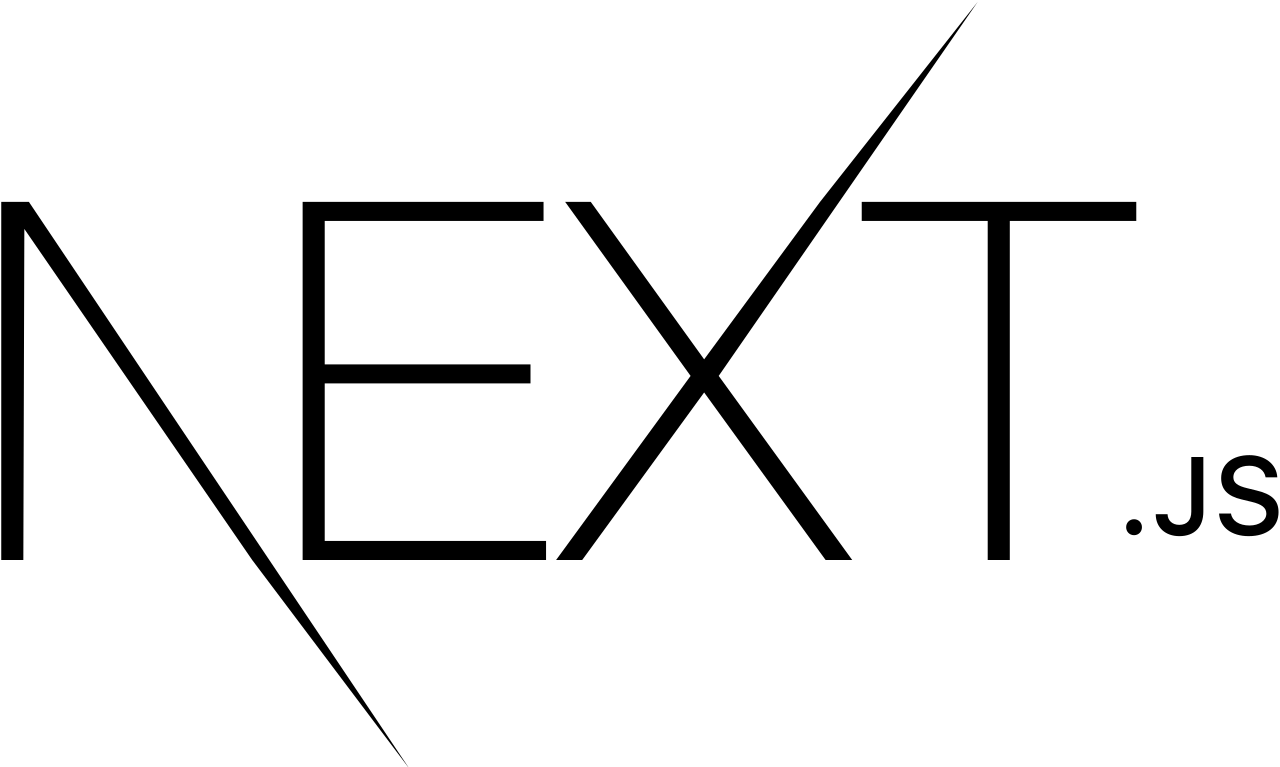
\includegraphics[width=0.2\textwidth]{assets/next-logo.png}
	\caption{NextJS logo}
\end{figure}
A NextJS project has to follow a certain structure. The NextJS bundler will create a new page for the application for each file that is created inside the \texttt{pages} folder. For example, in the \texttt{core} application, there are the following pages\footnote{Not all the folders have been included, as there are pages nested within other pages; it is a reduced folder structure.}:
\begin{verbatim}
apps/core/pages
├── pages
│   └── index.tsx
├── 404
├── _app.tsx
├── auth
│   ├── signup
│   │   └── index.tsx
│   └── login
│       └── index.tsx
├── clients
│   └── index.tsx
├── dashboard
│   └── index.tsx
├── _document.tsx
├── events
│   └── index.tsx
├── index.tsx
├── settings
│   └── index.tsx
├── trainers
│   └── index.tsx
├── virtual-gyms
│   └── index.tsx
└── workers
    └── index.tsx
\end{verbatim}
In this case, instead of defining files, I opted for the \texttt{<folder-name>/index.tsx} structure. NextJS will check for each folder and when it finds a file with the \texttt{index.tsx}\footnote{The files can end with \texttt{jsx} (JavaScript React file), \texttt{js} (JavaScript file) or \texttt{tsx} (TypeScript React file).}, generates the logic required to display the page in the URL of \texttt{<folder-name>}. If a folder is nested within another folder, as it is the case of the \texttt{auth} folder, the URL would be the same, but nested> \texttt{auth/signup} and \texttt{auth/login}. Aside from folders, there are special files which are specially treated by the NextJS compiler. For example, the \texttt{\_app.tsx} is the entry point of the application and the content of it will be the parent of each page\footnote{This is very useful for SEO purposes, as an example.}.
\\[8pt]
One of the other important features NextJS provides is \texttt{code-splitting} \cite{code-splitting}. Code splitting consists in splitting the content provided by the server to the chrome in different bundles. Therfore, when the user loads the website, instead of providing all HTML, CSS and JS files, it only recieves what is required. In React applications this is extremely handy, since the React content is provided as a single gigantic JavaScript file.
\subsubsection{Mui}
Once the web framework have been decided, the applications need to share a common user interface to provide the user experience of using the same product. Keeping such similarities can be difficult if the enterprise or company does not have a well-defined design system. Therefore, creating my own design system was out of scope, and a components' library, as they are called, was needed. Again, there are multiple libraries to be used, yet there is one that shines above all others, which is the \texttt{mui} library. The library is open-source and maintained by \texttt{mui-org} \cite{mui}.
\\[8pt]
This library is based on the Google Material design system. However, it has an extremely powerful API to define your own design system, without the need of starting from 0. The developer has the possibility to inject the customised theme to all the components of the API included in the library. Furthermore, it includes an icon pack, which are the same as in the Google Material.
\begin{figure}[H]
	\centering
	
\includegraphics[width=0.2\textwidth]{assets/mui-logo.png}
	\caption{Mui library's logo}
\end{figure}
\subsection{Back end - Server application}
For the backend application, many languages can be used. However, since NodeJS provides a runtime environment for JavaScript, which allows building applications outside the browser. So, with the help on Nx, the backend is also written in TypeScript.
\subsubsection{Database}
The application has many relationships, which would be harder to maintain in a NoSQL database. Therefore, using a relational database is a better solution. At the first glance, I opted for the MySQL database since it is one of the most used SQL databases, nowadays. However, I have more experience with PostgreSQL and I had no issues with it. In the end, the chosen database has been PostgreSQL \cite{postgresql}.
\begin{figure}[H]
	\centering
	
\includegraphics[width=0.2\textwidth]{assets/postgres-logo.png}
	\caption{PostgreSQL's logo}
\end{figure}
As explained before the database is run in a docker container. Viewing the data in the terminal is not an issue, yet pgAdmin is a graphic user interface which simplifies such visualisation. It is the equivalent of MySQL Workbench for PostgreSQL. With such tool, schemas in general can be simply viewed and edited. Additionally, the JetBrains DataGrip application has been also used, which has allowed to generate the ERD once the database was defined.
\subsubsection{ExpressJS}
ExpressJS is one of the many back-end frameworks that exist in the JavaScript world, nowadays. It is a minimal and flexible framework which provides a fast methodology to develop APIs. It is considered the most popular back-end framework of JavaScript, up to a point that other back-end meta-frameworks are ExpressJS based (an example is NestJS). As stated in their landing page, ExpressJs is a: \emph{Fast, unopinionated, minimalist web framework for Node.js} \cite{expressjs}.
\begin{figure}[H]
	\centering
	
\includegraphics[width=0.2\textwidth]{assets/express-logo.png}
	\caption{ExpressJS's logo}
\end{figure}
\subsubsection{TypeORM}
Finally, the TypeORM library is used to provide a bidirectional connection from the server to the database. TypeORM is a TypeScript ORM (\emph{object relational mapper}) whose goal is to provide an agnostic model-database mapping. By using TypeScript decorators and defining a connection, TypeORM will generate the entities or documents specified, depending on the database to which is connected. Such agnosticism allows to re-use the models with different databases \cite{typeorm}.
\begin{figure}[H]
	\centering
	
\includegraphics[width=0.3\textwidth]{assets/typeorm-logo.png}
	\caption{TypeORM's logo}
\end{figure}
In conjunction with Nx, the models that are used to generate the entities and their relations, can be used in the front-end applications. Therefore, such models can be shared and easily maintained.
\subsection{Tests}
Last but not least, the test stack also had to be defined. In this case, the provided frameworks for testing by Nx were kept, since they are some of the most common testing libraries nowadays.
\subsubsection{Unit testing - Jest}
Both \texttt{@nrwl/express} and \texttt{@nrwl/next} generators set up the application with Jest. Jest is an open-source unit and mock testing framework developed and maintained by Facebook. It is one of the most popular libraries nowadays, since it is extremely powerful and simple. It offers a powerful CLI tool to control the tests which has an interactive mode that allows the developer only to run \emph{affected} tests\footnote{Nx also takes care of running only affected tests.}. Other benefits of Jest are that require zero configuration and ensures isolation between tests. Isolation is extremely important when running tests, to ensure that each test does not influence other's results. As stated in their home page: \emph{Jest is a delightful JavaScript Testing Framework with a focus in simplicity} \cite{jest}.
\begin{figure}[H]
	\centering
	
\includegraphics[width=0.3\textwidth]{assets/jest-logo.png}
	\caption{Jest's logo}
\end{figure}
Therefore, Jest is used in all the applications to unit tests the services, controllers, components and so on from all the applications. Furthermore, since there is a GitHub Action, CI can be easliy acomplished.
\subsubsection{Unit testing - \texttt{@testing-library}}
Aside from unit testing API functions and so on, it is important to also test the different React components, ensuring they behave as expected. Again, there are multiple choices to develop component unit tests, yet the solution chosen is the one which is installed with \texttt{@nrlw/next}: \texttt{@testing-library}. This package provides an API to easily test React components. It is a very light library which uses functions on top of \texttt{react-dom} and \texttt{react-dom/test-utils}.
\begin{figure}[H]
	\centering
	
\includegraphics[width=0.2\textwidth]{assets/testing-library-logo.png}
	\caption{Testing library's logo}
\end{figure}
\subsubsection{Client e2e testing - Cypress}
Cypress is more than a tool for testing. It provides a graphical user interface to see what is being tested, where it fails and other features. It is an extremely powerful tool for UI testing, which has always been a difficult subject. As stated in their website, cypress enables you to: \emph{write faster, easier and more reliable tests} \cite{cypress}.
\begin{figure}[H]
	\centering
	
\includegraphics[width=0.3\textwidth]{assets/cypress-logo.png}
	\caption{Cypress's logo}
\end{figure}
In order to use cypress, the project needs a specific folder structure which can be a bit confusing to set up. However, the \texttt{@nrlw/next} plugin already sets up this environment, which is kept in the \texttt{*-e2e} folders\footnote{In the system case, the different cypress environments are in: \texttt{client-e2e}, \texttt{core-e2e} and \texttt{landing-e2e}.}.
\subsubsection{Server e2e testing - Jest and Supertest}
Finally, the libraries that are installed to develop end-to-end test for express, in \texttt{@nrwl/express} are: Jest and Supertest. The Jest library has already been covered. The Supertest is an HTTP assertions library that allows the developer to create Node.js HTTP tests. It uses the SuperAgent library, which is an HTTP client for Node.js. Using Supertest is one of the most common methods to develop such tests.
\chapter{Analysis and system design}
\section{Use case diagram}
% TODO: Explain that all relations are include
% TODO: Explain why it is divided in 3 diagrams
% TODO: Explain that worker permissions are not explained
\begin{figure}[H]
	\centering
	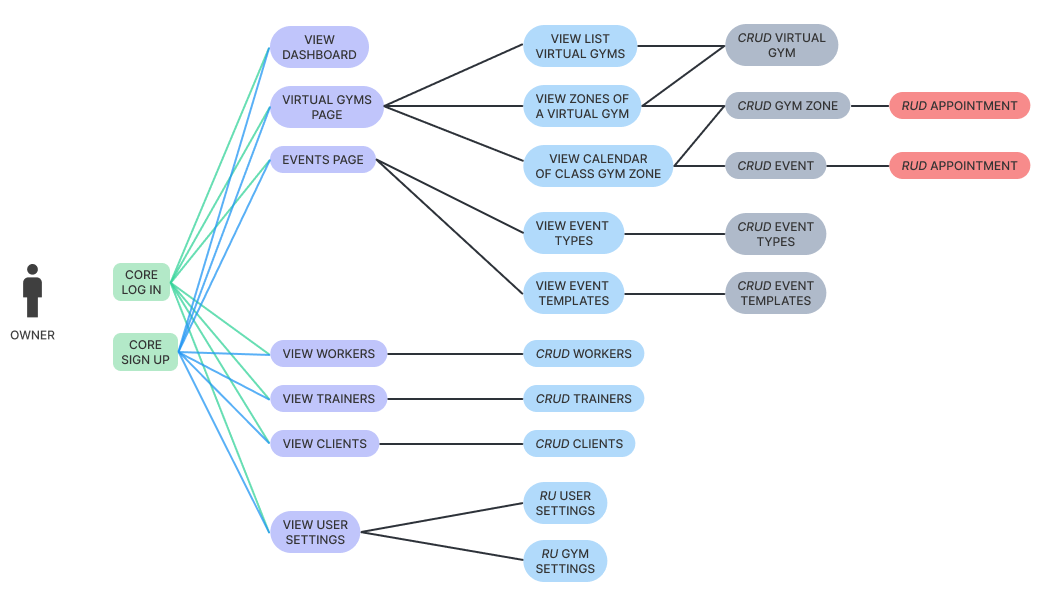
\includegraphics[width=\textwidth]{assets/use-case-diagrams/owner.png}
	\caption{Owner's core application use case diagram}
\end{figure}
The owner's use case diagram is the above one. It goes from left to right, and all relations are of type \emph{include}, meaning that you cannot move right without being in the left position before. It is also important to note, that it is also possible to move from right to left, for example, after creating a worker, the user is moved back to the \emph{view workers} state. The owner has access to all the possible states, as it is like a super user of the application (it is another reason on why all relations are \emph{include} type).
\\[8pt]
Another important point to notice is the \emph{CRUD} notation. I have opted for this notation in order to make the diagram smaller and also help with the interaction of the user. \emph{CRUD} stands for \emph{Create}, \emph{Read}, \emph{Update} and \emph{Delete}. For example, the \emph{CRUD Workers} state would be the possibility of \emph{creating}, \emph{reading}, \emph{updating} and \emph{deleting} workers. 
\section{Database diagram}
\subsection{Introduction}
In a previous section, it has been explained that the DataGrip application has been used to create the database diagram. The process to create such diagram has been:
\begin{enumerate}[label = \textbf{\arabic{*}.}]
	\item Create the entities with TypeORM. The synchronization of TypeORM with the empty database, will create all the tables, sequences, indexes and so on that have been defined. Therefore, the use of SQL is minimum and can easily be debugged, if needed.
	\item Set up a connection to the dockerized database with DataGrip.
	\item Generate the ERD with the detected tables.
\end{enumerate}
Such tool allows faster diagrams visualisation and avoids the pain of having to keep ERD diagrams manually updated on any minor change,
\subsection{Diagram}
The resulting diagram is:
\begin{figure}[H]
	\centering
	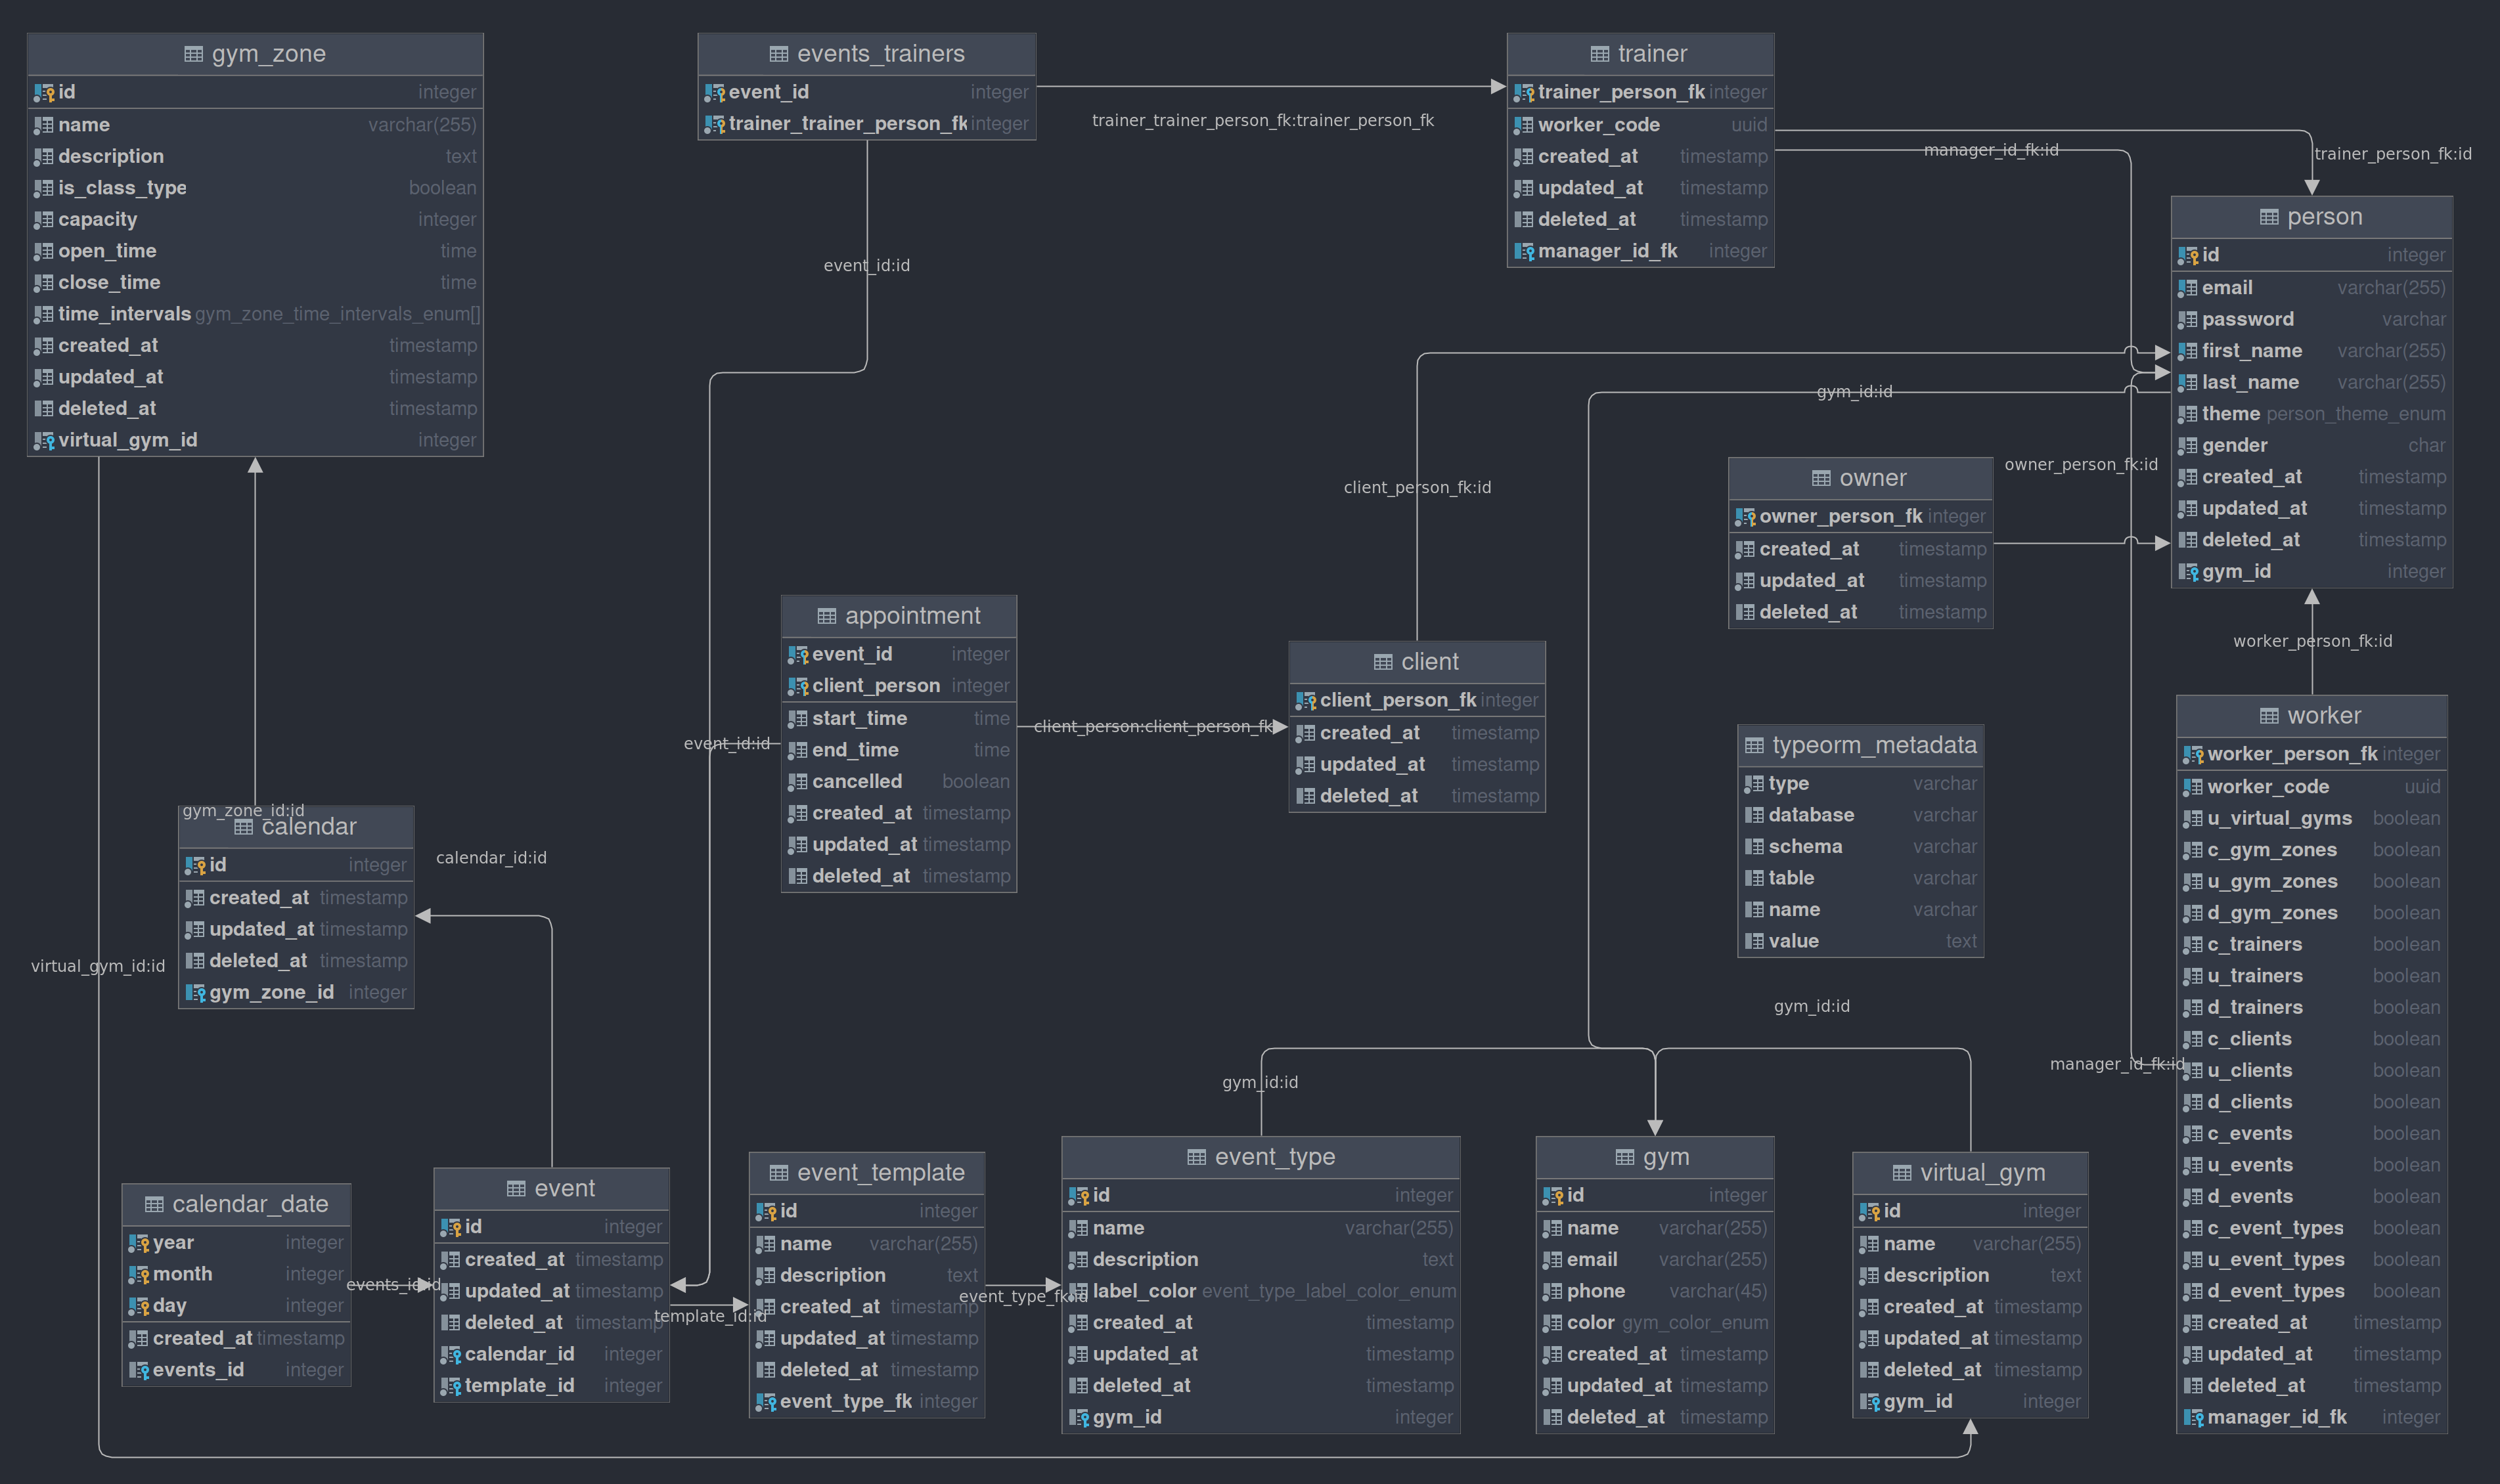
\includegraphics[width=\textwidth]{assets/db-erd.png}
	\caption{Database diagram}
\end{figure}
\subsubsection{Introduction}
In the following sections each table will be explained and a brief description of their fields will be given. Each field will be represented using the following schema:
\begin{enumerate}[label = -]
	\item \textbf{<field name>} (\texttt{<field type>}) [\texttt{<field constraints>}] \texttt{->} <field description>
\end{enumerate}
There are some fields that are common to the different entities, independently of their relations. Such fields are:
\begin{enumerate}[label = -]
	\item \textbf{created\_at} (\texttt{timestamp}) [\texttt{DEFAULT NOW()}] \texttt{->} Keeps the \emph{timestamp} at which the entity has been created.
	\item \textbf{updated\_at} (\texttt{timestamp}) [\texttt{DEFAULT NOW()}] \texttt{->} Keeps the \emph{timestamp} at which the entity has been last updated.
	\item \textbf{deleted\_at} (\texttt{timestamp}) [] \texttt{->} Keeps the \emph{timestamp} at which the entity has been dele-ted.
\end{enumerate}
\subsubsection{Person}
One of the big concepts to define in the database has been how are users stored. After comparing many approaches, a multiple table inheritance has been chosen. The base table of the user's inheritance is the \emph{Person}. The person entity will have an id which will be the primary key of the entities that inherit from the table. Such entity contains the mandatory data each user must have:
\begin{enumerate}[label = -]
	\item \textbf{id} (\texttt{integer}) [\texttt{PRIMARY KEY AUTOINCREMENT}] \texttt{->} This is the \emph{primary key} of the entity.
	\item \textbf{email} (\texttt{varchar(255)}) [\texttt{NOT NULL}] \texttt{->} Stores the email of the user. The email is indexed by a \emph{unique index} (\texttt{person-email-idx}).
	\item \textbf{password} (\texttt{varchar(255)}) [\texttt{NOT NULL}] \texttt{->} Stores the password of the user which is encrypted before insert.
	\item \textbf{first\_name} (\texttt{varchar(255)}) [\texttt{NOT NULL}] \texttt{->} Stores the first name of the user. This field is indexed for faster queries by first name (\texttt{person-first-name-idx}).
	\item \textbf{last\_name} (\texttt{varchar(255)}) [\texttt{NOT NULL}] \texttt{->} Stores the last name of the user. This field is indexed for faster queries by last name (\texttt{person-last-name-idx}).
	\item \textbf{theme} (\texttt{app\_theme}) [\texttt{DEFAULT "LIGHT"}] \texttt{->} Stores the theme used by the person in the different applications\footnote{This field is an enum defined in the library \texttt{@hubbl/shared/enums}.}.
	\item \textbf{gender} (\texttt{char}) [\texttt{NOT NULL}] \texttt{->} Stores the gender of the person.
	\item \textbf{gym\_id} (\texttt{integer}) [\texttt{NOT NULL}] \texttt{->} Stores the id of the \texttt{Gym} entity to which the user belongs.
\end{enumerate}
\subsubsection{Owner}
The \emph{Owner} entity is the person who has the most permissions. Therefore, instead of having all the permissions which are defined in the \emph{Worker} entity set to \texttt{true}, the \emph{Owner}'s are kept in a different table. Additionally, an owner will have more permissions than the ones stored in the \emph{Worker} entity. The fields of the table are:
\begin{enumerate}[label = -]
	\item \textbf{person\_id} (\texttt{integer}) [\texttt{PRIMARY KEY AUTOINCREMENT}] \texttt{->} References an id of the \emph{Person} entity.
	\item \textbf{onwer\_id} (\texttt{integer}) [] \texttt{->} References the id of the \emph{Gym} the owner owns.
\end{enumerate}
\subsubsection{Worker}
The next person type is the \emph{Worker}. A worker has different permissions set by the owner when created. The \emph{Worker} entity basically contains \texttt{boolean} fields which allow the system to know what permissions have been given to the worker. The permissions of the user are set using the following rule: \texttt{<operation>\_<on>}. For example, the permission of \emph{updating} the gym zones is \texttt{update\_gym\_zone}.
\\[8pt]
The fields of the table are
\begin{enumerate}[label = -]
	\item \textbf{person\_id} (\texttt{integer}) [\texttt{PRIMARY KEY AUTOINCREMENT}] \texttt{->} References an id of the \emph{Person} entity.
	\item \textbf{update\_virtual\_gym} (\texttt{boolean}) [\texttt{DEFAULT FALSE NOT NULL}] \texttt{->} Permission to update a \emph{VirtualGym}.
	\item \textbf{create\_gym\_zones} (\texttt{boolean}) [\texttt{DEFAULT FALSE NOT NULL}] \texttt{->} Permission to create a \emph{GymZone}.
	\item \textbf{update\_gym\_zones} (\texttt{boolean}) [\texttt{DEFAULT FALSE NOT NULL}] \texttt{->} Permission to update a \emph{GymZone}.
	\item \textbf{delete\_gym\_zones} (\texttt{boolean}) [\texttt{DEFAULT FALSE NOT NULL}] \texttt{->} Permission to\\delete a \emph{GymZone}.
	\item \textbf{create\_trainers} (\texttt{boolean}) [\texttt{DEFAULT FALSE NOT NULL}] \texttt{->} Permission to create a \emph{Trainer}.
	\item \textbf{update\_trainers} (\texttt{boolean}) [\texttt{DEFAULT FALSE NOT NULL}] \texttt{->} Permission to update a \emph{Trainer}.
	\item \textbf{delete\_trainers} (\texttt{boolean}) [\texttt{DEFAULT FALSE NOT NULL}] \texttt{->} Permission to delete a \emph{Trainer}.
	\item \textbf{create\_clients} (\texttt{boolean}) [\texttt{DEFAULT FALSE NOT NULL}] \texttt{->} Permission to create a\\\emph{Client}.
	\item \textbf{update\_clients} (\texttt{boolean}) [\texttt{DEFAULT FALSE NOT NULL}] \texttt{->} Permission to update a \emph{Client}.
	\item \textbf{delete\_clients} (\texttt{boolean}) [\texttt{DEFAULT FALSE NOT NULL}] \texttt{->} Permission to delete a\\\emph{Client}.
	\item \textbf{create\_tags} (\texttt{boolean}) [\texttt{DEFAULT FALSE NOT NULL}] \texttt{->} Permission to create a\\\emph{TrainerTag}.
	\item \textbf{update\_tags} (\texttt{boolean}) [\texttt{DEFAULT FALSE NOT NULL}] \texttt{->} Permission to update a \emph{TrainerTag}.
	\item \textbf{delete\_tags} (\texttt{boolean}) [\texttt{DEFAULT FALSE NOT NULL}] \texttt{->} Permission to delete a\\\emph{TrainerTag}.
	\item \textbf{create\_events} (\texttt{boolean}) [\texttt{DEFAULT FALSE NOT NULL}] \texttt{->} Permission to create an \emph{Event}.
	\item \textbf{update\_events} (\texttt{boolean}) [\texttt{DEFAULT FALSE NOT NULL}] \texttt{->} Permission to update an \emph{Event}.
	\item \textbf{delete\_events} (\texttt{boolean}) [\texttt{DEFAULT FALSE NOT NULL}] \texttt{->} Permission to\\delete an \emph{Event}.
	\item \textbf{create\_event\_types} (\texttt{boolean}) [\texttt{DEFAULT FALSE NOT NULL}] \texttt{->} Permission to create an \emph{EventType}.
	\item \textbf{update\_event\_types} (\texttt{boolean}) [\texttt{DEFAULT FALSE NOT NULL}] \texttt{->} Permission to update an \emph{EventType}.
	\item \textbf{delete\_event\_types} (\texttt{boolean}) [\texttt{DEFAULT FALSE NOT NULL}] \texttt{->} Permission to\\delete an \emph{EventType}.
	\item \textbf{create\_event\_templates} (\texttt{boolean}) [\texttt{DEFAULT FALSE NOT NULL}] \texttt{->} Permission to create an \emph{EventTemplate}.
	\item \textbf{update\_event\_templates} (\texttt{boolean}) [\texttt{DEFAULT FALSE NOT NULL}] \texttt{->} Permission to update an \emph{EventTemplate}.
	\item \textbf{delete\_event\_templates} (\texttt{boolean}) [\texttt{DEFAULT FALSE NOT NULL}] \texttt{->} Permission to\\delete an \emph{EventTemplate}.
	\item \textbf{create\_event\_appointments} (\texttt{boolean}) [\texttt{DEFAULT FALSE NOT NULL}] \texttt{->} Permission to create an \emph{EventAppointment}.
	\item \textbf{update\_event\_appointments} (\texttt{boolean}) [\texttt{DEFAULT FALSE NOT NULL}] \texttt{->} Permission to update an \emph{EventAppointment}.
	\item \textbf{delete\_event\_appointments} (\texttt{boolean}) [\texttt{DEFAULT FALSE NOT NULL}] \texttt{->} Permission to\\delete an \emph{EventAppointment}.
	\item \textbf{create\_calendar\_appointments} (\texttt{boolean}) [\texttt{DEFAULT FALSE NOT NULL}] \texttt{->} Permission to create a \emph{CalendarAppointment}.
	\item \textbf{update\_calendar\_appointments} (\texttt{boolean}) [\texttt{DEFAULT FALSE NOT NULL}] \texttt{->} Permission to update a \emph{CalendarAppointment}.
	\item \textbf{delete\_calendar\_appointments} (\texttt{boolean}) [\texttt{DEFAULT FALSE NOT NULL}] \texttt{->} Permission to delete a \emph{CalendarAppointment}.
	\item \textbf{manager\_id\_fk} (\texttt{integer}) [\texttt{NOT NULL}] \texttt{->} References the manager (\emph{Owner}) of the \emph{Worker}.
\end{enumerate}
\subsubsection{Trainer}
The trainer table is very simple since it has no interaction with the system. It is a subset of the properties of a worker.
\begin{enumerate}[label = -]
	\item \textbf{person\_id} (\texttt{integer}) [\texttt{PRIMARY KEY AUTOINCREMENT}] \texttt{->} References an id of the \emph{Person} entity.
\end{enumerate}
\subsubsection{Client}
Client is a WIP entity.
\begin{enumerate}[label = -]
	\item \textbf{person\_id} (\texttt{integer}) [\texttt{PRIMARY KEY AUTOINCREMENT}] \texttt{->} References an id of the \emph{Person} entity.
	\item \textbf{covid\_passport} (\texttt{boolean}) [\texttt{NOT NULL DEFAULT FALSE}] \texttt{->} Allows the gym owners and workers to know if the user has registered the covid passport.
\end{enumerate}
\subsubsection{Gym}
The \emph{Gym} entity is relates to the company, not the infrastructure of a gym. Therefore, it works as a bridge entity that knows the preferences of the gym, such as the interface, gym location and other data. These properties can only be modified by an owner person. The table consists of the following fields:
\begin{enumerate}[label = -]
	\item \textbf{id} (\texttt{integer}) [\texttt{PRIMARY KEY AUTOINCREMENT}] \texttt{->} Unique id of the \emph{Gym}.
	\item \textbf{name} (\texttt{varchar(255)}) [\texttt{NOT NULL}] \texttt{->} Name of the \emph{Gym}, which will be displayed to the client and workers.
	\item \textbf{email} (\texttt{varchar(255)}) [\texttt{NOT NULL}] \texttt{->} Contact email of the \emph{Gym}.
	\item \textbf{phone} (\texttt{varchar(255)}) [\texttt{NOT NULL}] \texttt{->} Contact phone of the \emph{Gym}.
	\item \textbf{code} (\texttt{varchar(8)}) [\texttt{NOT NULL}] \texttt{->} Unique \emph{Gym} code used to identify the gym so the \emph{Client} can use it when registering to the application.
	\item \textbf{color} (\texttt{theme\_color}) [\texttt{DEFAULT "\#2196F3" NOT NULL}] \texttt{->} Primary color of the gym which is the same with all the users\footnote{This field is an enum defined in the library \texttt{@hubbl/shared/enums}.}.
\end{enumerate}
\subsubsection{VirtualGym}
Once the \emph{Gym} has been defined, the company may have multiple different infrastructures, for example, if it is a franchise. These virtual gyms are stored in the \emph{VirtualGym} table. The virtual gym will have different constraints which can change if the workers or owners do change them. The fields of the \emph{VirtualGym} table are:
\begin{enumerate}[label = -]
	\item \textbf{id} (\texttt{integer}) [\texttt{PRIMARY KEY AUTOINCREMENT}] \texttt{->} Unique id of the \emph{VirtualGym}.
	\item \textbf{name} (\texttt{varchar(255)}) [\texttt{NOT NULL}] \texttt{->} Name of the \emph{VirtualGym}.
	\item \textbf{description} (\texttt{text}) [\texttt{NOT NULL}] \texttt{->} Description of the \emph{VirtualGym}.
	\item \textbf{location} (\texttt{varchar(255)}) [\texttt{NOT NULL}] \texttt{->} Location of the \emph{VirtualGym}.
	\item \textbf{capacity} (\texttt{integer}) [\texttt{NOT NULL}] \texttt{->} Maximum capacity of the \emph{VirtualGym}.
	\item \textbf{phone} (\texttt{integer}) [] \texttt{->} Optional phone of the \emph{VirtualGym}.
	\item \textbf{open\_time} (\texttt{time}) [\texttt{NOT NULL}] \texttt{->} Time at which the \emph{VirtualGym} opens.
	\item \textbf{close\_time} (\texttt{time}) [\texttt{NOT NULL}] \texttt{->} Time at which the \emph{VirtualGym} closes.
	\item \textbf{gym\_id} (\texttt{integer}) [\texttt{NOT NULL}] \texttt{->} \emph{Gym} to which the \emph{VirtualGym} belongs.
\end{enumerate}
\subsubsection{GymZone}
After having created the \emph{VirtualGym}, now gym zones can be created for the different virtual gyms of a gym. There are two types of zones: class and non-class zones. The class zones will have a schedule with \emph{Event}'s create by the gym personnel, while non-class zones will have a schedule without events. At the same time, it has the constraints set by the owner and workers, similar to the \emph{VirtualGym}.
\\[8pt]
The columns of the entity are:
\begin{enumerate}[label = -]
	\item \textbf{id} (\texttt{integer}) [\texttt{PRIMARY KEY AUTOINCREMENT}] \texttt{->} Unique id of the \emph{GymZone}.
	\item \textbf{name} (\texttt{varchar(255)}) [\texttt{NOT NULL}] \texttt{->} Name of the \emph{GymZone}.
	\item \textbf{description} (\texttt{text}) [\texttt{NOT NULL}] \texttt{->} Description of the \emph{GymZone}.
	\item \textbf{is\_class\_type} (\texttt{boolean}) [\texttt{DEFAULT FALSE}] \texttt{->} Whether it is a class or non-class zone.
	\item \textbf{capacity} (\texttt{integer}) [\texttt{NOT NULL}] \texttt{->} Maximum capacity of the \emph{GymZone}.
	\item \textbf{mask\_required} (\texttt{boolean}) [\texttt{NOT NULL DEFAULT TRUE}] \texttt{->} Whether wearing the mask is mandatory to access the \emph{GymZone}.
	\item \textbf{covid\_passport} (\texttt{boolean}) [\texttt{NOT NULL DEFAULT TRUE}] \texttt{->} Whether having registered the covid passport is mandatory to access the \emph{GymZone}.
	\item \textbf{open\_time} (\texttt{time}) [\texttt{NOT NULL}] \texttt{->} Time at which the \emph{GymZone} opens.
	\item \textbf{close\_time} (\texttt{time}) [\texttt{NOT NULL}] \texttt{->} Time at which the \emph{GymZone} closes.
	\item \textbf{time\_intervals} (\texttt{time\_interval[]}) [\texttt{DEFAULT {30, 60, 90, 120}}] \texttt{->} This field will only be used if the \emph{GymZone} is a non-class zone. It defines the time intervals, in minutes, that the clients will be able to make the appointments.
	\item \textbf{calendar\_id} (\texttt{integer}) [\texttt{NOT NULL}] \texttt{->} \emph{Calendar} identifier of the \emph{GymZone}.
	\item \textbf{virtual\_gym\_id} (\texttt{integer}) [\texttt{NOT NULL}] \texttt{->} \emph{VirtualGym} to which the \emph{GymZone} belongs.
\end{enumerate}
\subsubsection{Calendar}
The \emph{Calendar} entity is linked to a \emph{GymZone} and is used to link the events and to know how many clients have made an \emph{Appointment} during a time interval. The \emph{Calendar} will always be linked with \emph{Event}'s, and the \emph{Event} entity will be used to determine if the \emph{Appointment} is for a class or a non-class zone.
\\[8pt]
The fields of the table are:
\begin{enumerate}[label = -]
	\item \textbf{id} (\texttt{integer}) [\texttt{PRIMARY KEY AUTOINCREMENT}] \texttt{->} Unique id of the \emph{Calendar}.
\end{enumerate}
\subsubsection{CalendarDate}
A \emph{CalendarDate} is a simple entity that will contain the year, month and day of a date. It will be created \emph{on demand}, meaning that each entry is unique, yet it will not exist until there is another entity that requires of it. With this approach, the system avoids the need to fill the table with hundreds of entries for each date. The fields are:
\begin{enumerate}[label = -]
	\item \textbf{year} (\texttt{integer}) [\texttt{NOT NULL}] \texttt{->} Year of the \emph{CalendarDate}.
	\item \textbf{month} (\texttt{integer}) [\texttt{NOT NULL}] \texttt{->} Month of the \emph{CalendarDate}.
	\item \textbf{day} (\texttt{integer}) [\texttt{NOT NULL}] \texttt{->} Day of the \emph{CalendarDate}.
\end{enumerate}
In order to ensure each entry is unique, a \emph{composite unique index} has been set which contains the three fields of the table.
\subsubsection{EventType}
The system allows the user to create events are of a specific type. For instance, the types can be: spinning, zumba, yoga and so on. There will be predefined \emph{EventType}'s when the owner first creates the gym. However, in order to allow more flexibility while using the application, the system also allows the user to create custom \emph{EventType}'s.
\\[8pt]
The \emph{EventType} entity is composed by the following columns:
\begin{enumerate}[label = -]
	\item \textbf{id} (\texttt{integer}) [\texttt{PRIMARY KEY AUTOINCREMENT}] \texttt{->} Unique id of the \emph{EventType}.
	\item \textbf{name} (\texttt{varchar(255)}) [\texttt{NOT NULL}] \texttt{->} Name of the \emph{EventType}.
	\item \textbf{description} (\texttt{text}) [\texttt{NOT NULL}] \texttt{->} Description for the \emph{EventType}.
	\item \textbf{label\_color} (\texttt{app\_palette}) [\texttt{DEFAULT "\#2196F3" NOT NULL}] \texttt{->} Color of the \emph{EventType} when displayed.
	\item \textbf{gym\_id} (\texttt{integer}) [\texttt{NOT NULL}] \texttt{->} References the id to which the \emph{EventType} belongs.
\end{enumerate}
\subsubsection{EventTemplate}
In order to reduce the repetitive process of creating \emph{Event}'s for a gym zone, the system provides the utility of creating \emph{EventTemplate}'s, which allow the owners or workers to create \emph{Event}'s faster. With the \emph{EventTemplate} utility, in order to create an \emph{Event} becomes faster and less repetitive.
\\[8pt]
The fields of this entity are:
\begin{enumerate}[label = -]
	\item \textbf{id} (\texttt{integer}) [\texttt{PRIMARY KEY AUTOINCREMENT}] \texttt{->} Unique id of the \emph{EventTemplate}.
	\item \textbf{name} (\texttt{varchar(255)}) [\texttt{NOT NULL}] \texttt{->} Name of the \emph{EventTemplate}.
	\item \textbf{description} (\texttt{text}) [\texttt{NOT NULL}] \texttt{->} Description for the \emph{EventTemplate}.
	\item \textbf{capacity} (\texttt{integer}) [\texttt{NOT NULL}] \texttt{->} Optional description for the \emph{EventTemplate}.
	\item \textbf{covid\_passport} (\texttt{integer}) [\texttt{NOT NULL DEFAULT FALSE}] \texttt{->} Whether the event will require the client to have the covid passport or not.
	\item \textbf{mask\_required} (\texttt{integer}) [\texttt{NOT NULL DEFAULT FALSE}] \texttt{->} Whether the event will require the client to wear a mask.
	\item \textbf{event\_type\_fk} (\texttt{integer}) [] \texttt{->} References the \emph{EventType} of the \emph{EventTemplate}.
	\item \textbf{gym\_id} (\texttt{integer}) [\texttt{NOT NULL}] \texttt{->} References the \emph{EventType} of the \emph{EventTemplate}.
\end{enumerate}
\subsubsection{Event}
Finally, the \emph{Event} can be defined. An \emph{Event} is a bridge table that contains: the \emph{Trainer}, the \emph{CalendarDate}, the \emph{Calendar} to which is scheduled and the \emph{EventTemplate}. All these identify the \emph{Event}, that is what the entity to which the user will be able to create an appointment.
\\[8pt]
The table is defined as:
\begin{enumerate}[label = -]
	\item \textbf{id} (\texttt{integer}) [\texttt{PRIMARY FIELD NOT NULL}] \texttt{->} Unique identifier of the \emph{Event}.
	\item \textbf{name} (\texttt{varchar(255)}) [\texttt{NOT NULL}] \texttt{->} Name of the \emph{Event}.
	\item \textbf{description} (\texttt{text}) [\texttt{NOT NULL}] \texttt{->} Description for the \emph{Event}.
	\item \textbf{capacity} (\texttt{integer}) [\texttt{NOT NULL}] \texttt{->} Optional description for the \emph{Event}.
	\item \textbf{covid\_passport} (\texttt{integer}) [\texttt{NOT NULL DEFAULT FALSE}] \texttt{->} Whether the event will require the \emph{Client} to have the covid passport or not.
	\item \textbf{mask\_required} (\texttt{integer}) [\texttt{NOT NULL DEFAULT FALSE}] \texttt{->} Whether the event will require the \emph{Client} to wear a mask.
	\item \textbf{start\_time} (\texttt{time}) [\texttt{NOT NULL}] \texttt{->} Time at which the \emph{Event} starts.
	\item \textbf{end\_time} (\texttt{time}) [\texttt{NOT NULL}] \texttt{->} Time at which the \emph{Event} ends.
	\item \textbf{trainer\_person\_id} (\texttt{integer}) [\texttt{NOT NULL}] \texttt{->} References the \emph{Trainer} of the \emph{Event}.
	\item \textbf{calendar\_id} (\texttt{integer}) [\texttt{NOT NULL}] \texttt{->} References the \emph{Calendar} of the \emph{Event}.
	\item \textbf{template\_id} (\texttt{integer}) [] \texttt{->} References the \emph{EventTemplate} of the \emph{Event}, if any.
	\item \textbf{event\_type\_id} (\texttt{integer}) [] \texttt{->} References the \emph{EventType} of the \emph{Event}.
	\item \textbf{date\_year} (\texttt{integer}) [\texttt{NOT NULL}] \texttt{->} References the year of a \emph{CalendarDate} of the \emph{Event}.
	\item \textbf{date\_month} (\texttt{integer}) [\texttt{NOT NULL}] \texttt{->} References the month of a \emph{CalendarDate} of the \emph{Event}.
	\item \textbf{date\_day} (\texttt{integer}) [\texttt{NOT NULL}] \texttt{->} References the day of a \emph{CalendarDate} of the \emph{Event}.
\end{enumerate}
\subsubsection{EventAppointment and CalendarAppointment}
Finally, the only requirement left is the appointments from the \emph{Client}'s. The \emph{Client} has to be able to book a session for a guided class, which means to an \emph{Event}, or for a non-guided class, that is for a \emph{Calendar}. So, the two entities represent each case respectively. They both share some attributes, such as the \texttt{startTime} and the \texttt{openTime}. However, the \emph{EventAppointment} is related with an \emph{Event}, as it will be an \emph{Appointment} made to an \emph{Event}. On the other hand, a \emph{CalendarAppointment} would be an \emph{Appointment} made in a time interval, chosen by the user, for a specific \emph{GymZone}.
\\[8pt]
The fields of the \emph{EventAppointment} entity are:
\begin{enumerate}[label = -]
	\item \textbf{id} (\texttt{integer}) [\texttt{PRIMARY KEY NOT NULL}] \texttt{->} Unique identifier of the \emph{EventAppointment}
	\item \textbf{client\_person\_id} (\texttt{integer}) [\texttt{NOT NULL}] \texttt{->} References the \emph{Client} that has made the \emph{EventAppointment}.
	\item \textbf{event\_id} (\texttt{integer}) [\texttt{NOT NULL}] \texttt{->} References the \emph{Event} to which the \emph{EventAppointment} has been made.
	\item \textbf{start\_time} (\texttt{time}) [\texttt{NOT NULL}] \texttt{->} Time at which the \emph{EventAppointment} starts, which will be the same as the \emph{Event}.
	\item \textbf{end\_time} (\texttt{time}) [\texttt{NOT NULL}] \texttt{->} Time at which the \emph{EventAppointment} ends, which will be the same as the \emph{Event}.
	\item \textbf{cancelled} (\texttt{boolean}) [\texttt{NOT NULL DEFAULT FALSE}] \texttt{->} Used to know if the \emph{EventAppointment} has been cancelled.
\end{enumerate}
The fields of the \emph{CalendarAppointment} entity are:
\begin{enumerate}[label = -]
	\item \textbf{id} (\texttt{integer}) [\texttt{PRIMARY KEY NOT NULL}] \texttt{->} Unique identifier of the \emph{CalendarAppointment}
	\item \textbf{client\_person} (\texttt{integer}) [\texttt{NOT NULL}] \texttt{->} References the \emph{Client} that has made the \emph{CalendarAppointment}.
	\item \textbf{calendar\_id} (\texttt{integer}) [\texttt{NOT NULL}] \texttt{->} References the \emph{Calendar} to which the \emph{CalendarAppointment} has been made.
	\item \textbf{start\_time} (\texttt{time}) [\texttt{NOT NULL}] \texttt{->} Time at which the \emph{CalendarAppointment} starts.
	\item \textbf{end\_time} (\texttt{time}) [\texttt{NOT NULL}] \texttt{->} Time at which the \emph{CalendarAppointment} ends.
	\item \textbf{cancelled} (\texttt{boolean}) [\texttt{NOT NULL DEFAULT FALSE}] \texttt{->} Used to know if the \emph{CalendarAppointment} has been cancelled.
	\item \textbf{date\_year} (\texttt{integer}) [\texttt{NOT NULL}] \texttt{->} References the year of a \emph{CalendarDate} of the \emph{CalendarAppointment}.
	\item \textbf{date\_month} (\texttt{integer}) [\texttt{NOT NULL}] \texttt{->} References the month of a \emph{CalendarDate} of the \emph{CalendarAppointment}.
	\item \textbf{date\_day} (\texttt{integer}) [\texttt{NOT NULL}] \texttt{->} References the day of a \emph{CalendarDate} of the \emph{CalendarAppointment}.
\end{enumerate}
\section{User interfaces}
The design of the user interfaces has been a priority before diving into the front end development. Such interfices, provide a preliminar view of what show the application look and feel. The following figures, are the designs of the user interfaces that have been designed using the Figma software\footnote{The figma application is a free software which can be found in: \href{www.figma.com}{www.figma.com}}.
\\
Designing every possible state of the application is far from achievable with such little time. However, since the core and client application will share much of their user interface, only the core views have been designed. When developing the client application, most of the components have been reused, modifying they behaviour as needed, since the client interactions are limited (for instance, the client sees the same dashboard page, yet the button to add a virtual gym is hidden). Needless to say, some views do not correspond exactly as they are in the application, mainly because some features have been modified or added as required.
\\
Finally, the following aspects have been considered when designing the views:
\begin{enumerate}[label = -]
	\item The views should also be displayed as an owner used. This is due to the fact that the only differences between the views of an owner, a worker or a client, will be minimal. Some things will be hidden or not allowed, which has little effects to the final design.
	\item Each element that can be created (virtual gyms, gym zones, trainers and so on) must have their corresponding dialog or view in which such items are created, edited or deleated.
	      \begin{enumerate}[label = -]
		      \item In case a dialog is used, it has to contain how it looks when: it is being created, it is being edited, and it is being loaded, for each of the previous states.
	      \end{enumerate}
\end{enumerate}
With these requirements, there are views modals that contain 4 images, each one for the described states.
\\
% #region Images
\begin{figure}[H]
	\centering
	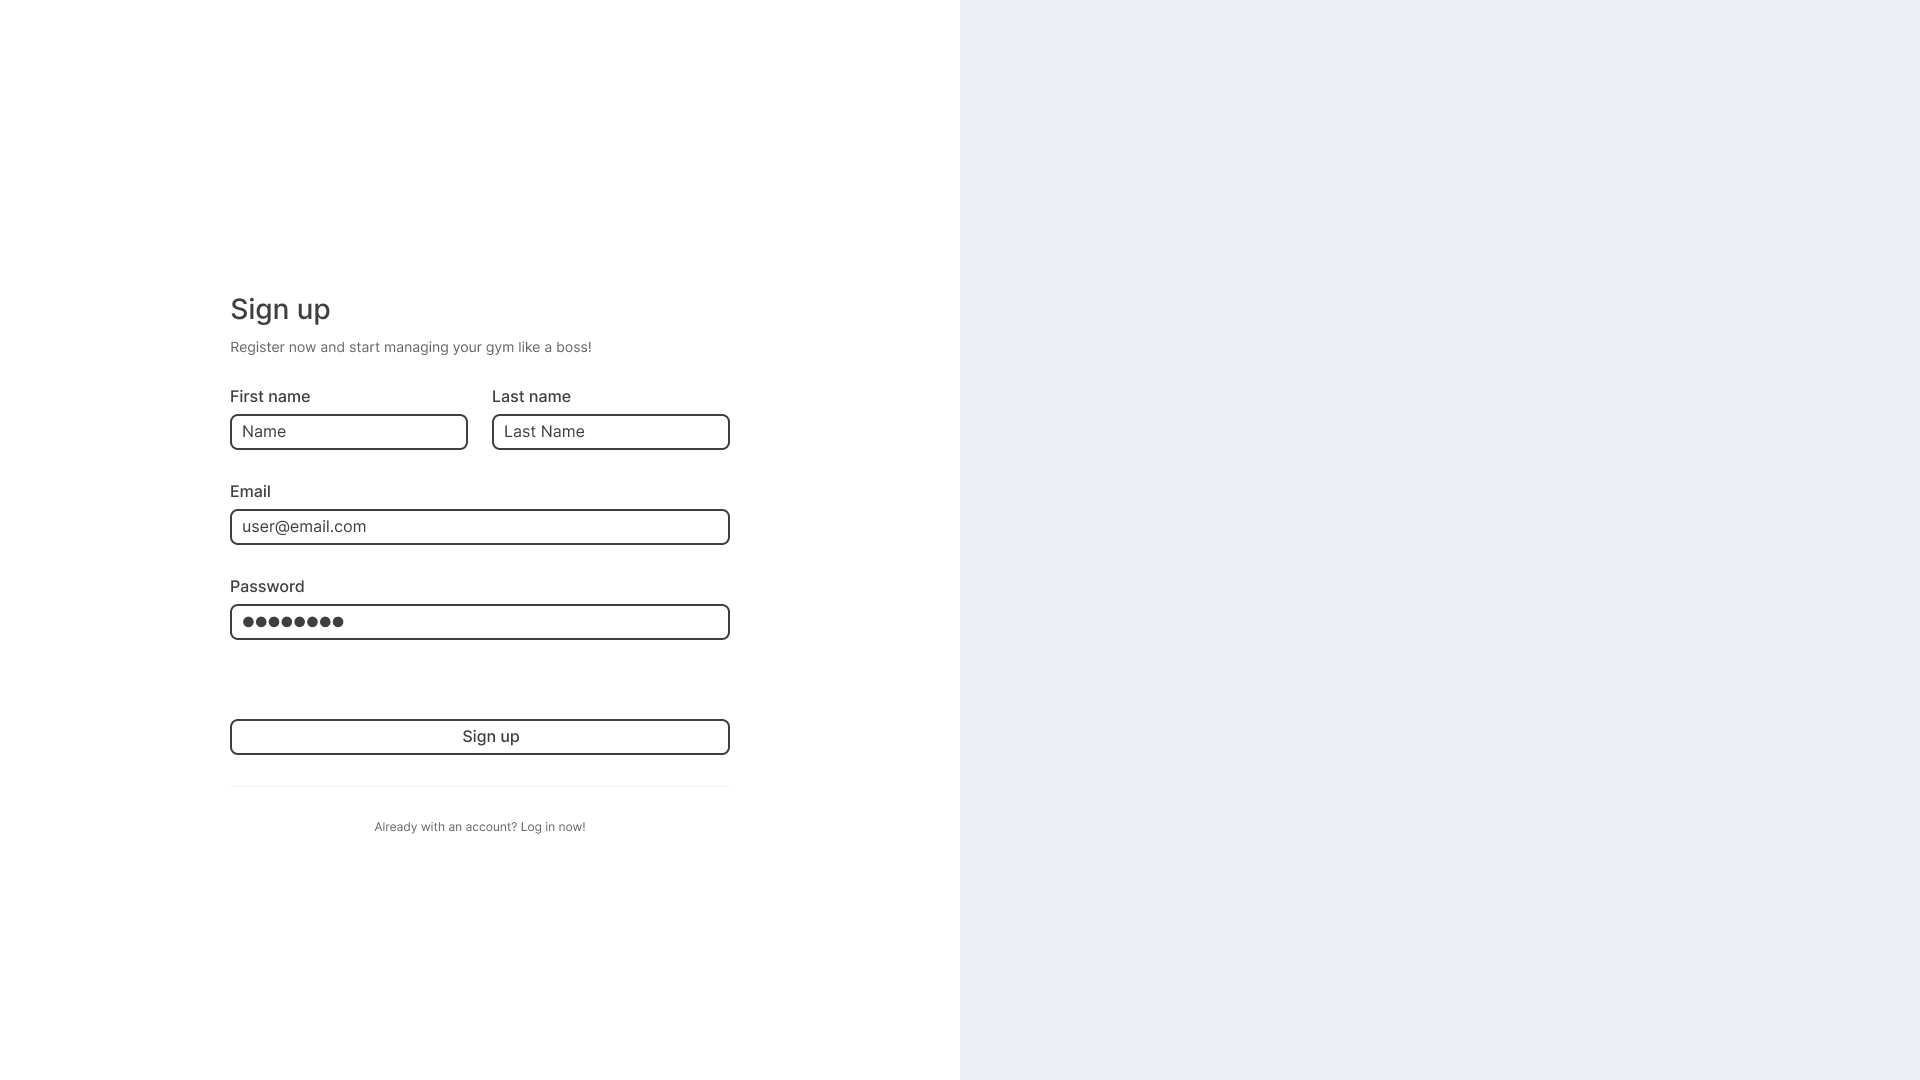
\includegraphics[width=\textwidth]{assets/ui/sign-up-step-one.png}
	\caption{First step of the sign up page}
\end{figure}
\begin{figure}[H]
	\centering
	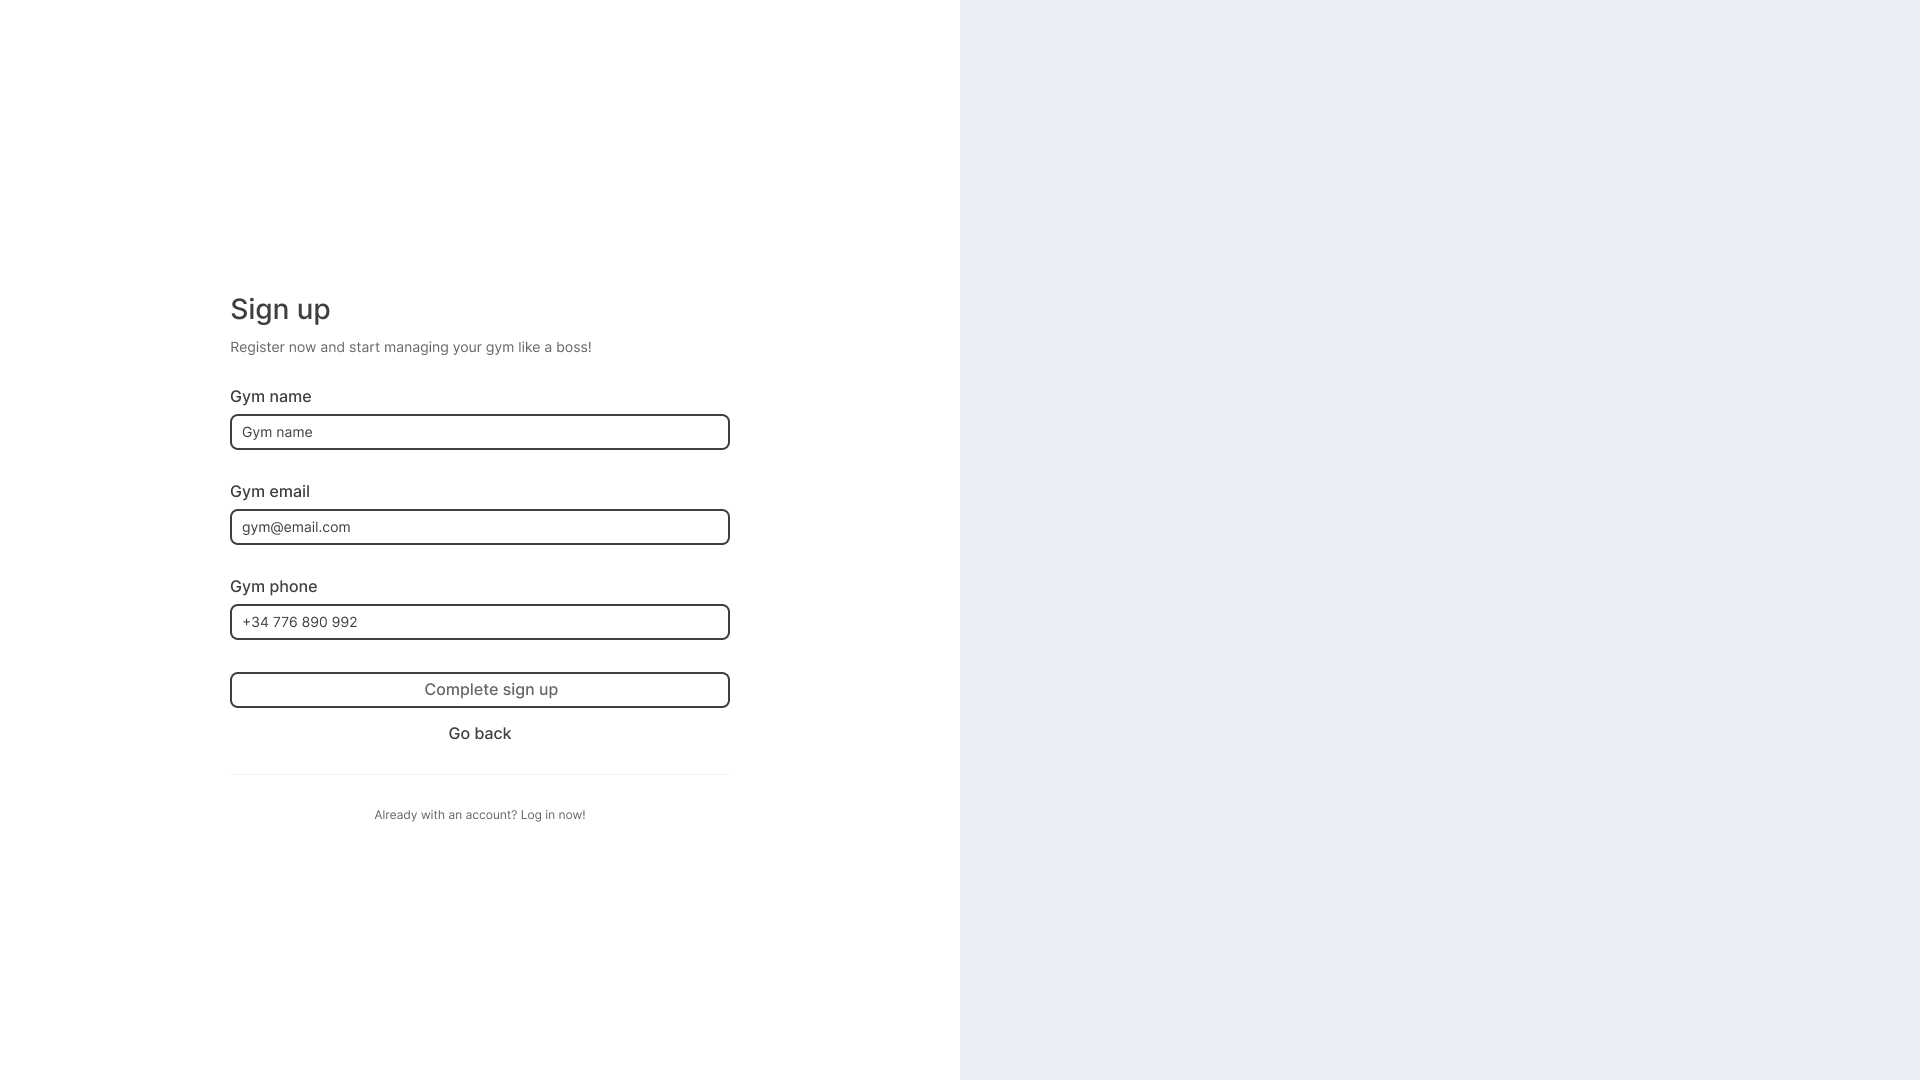
\includegraphics[width=\textwidth]{assets/ui/sign-up-step-two.png}
	\caption{Second step of the sign up page}
\end{figure}
\begin{figure}[H]
	\centering
	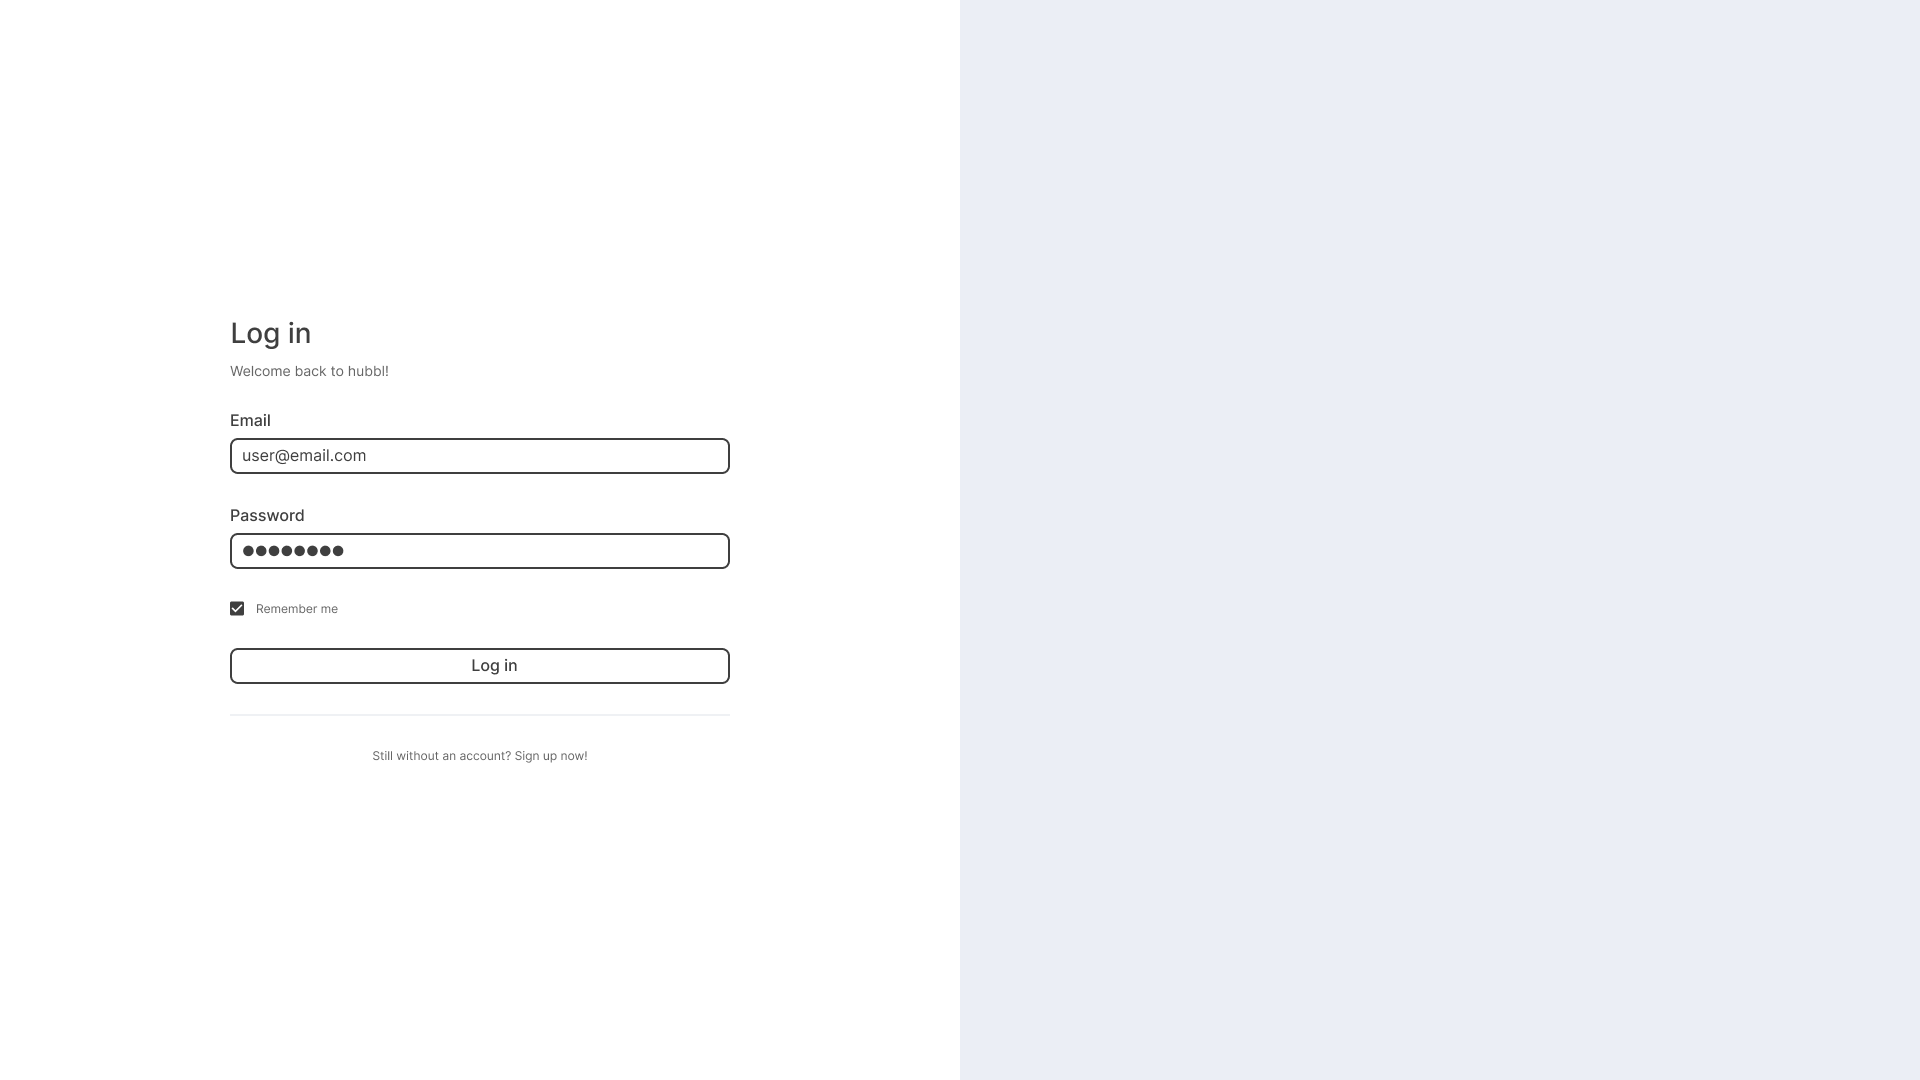
\includegraphics[width=\textwidth]{assets/ui/log-in.png}
	\caption{View of the login page}
\end{figure}
\begin{figure}[H]
	\centering
	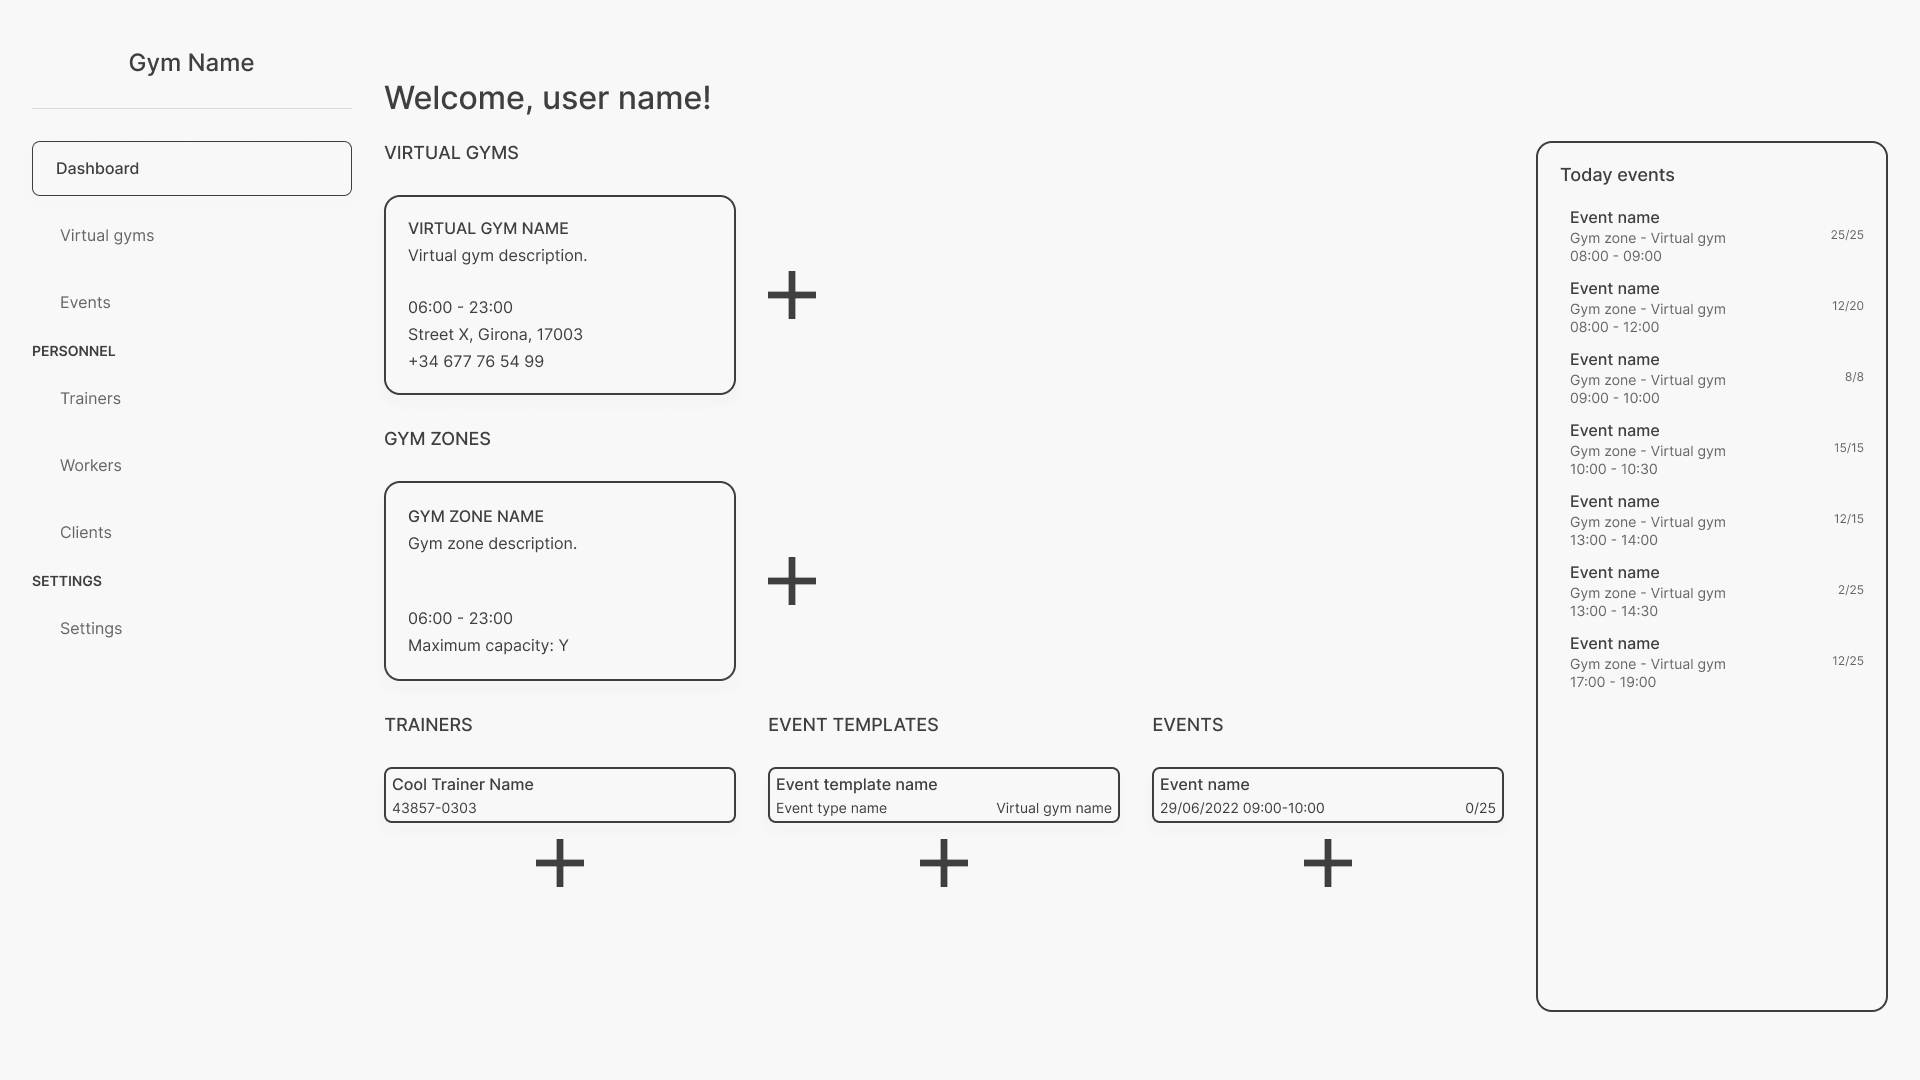
\includegraphics[width=\textwidth]{assets/ui/dashboard.png}
	\caption{Dashboard page, displaying a summary of the gym's information}
\end{figure}
\begin{figure}[H]
	\centering
	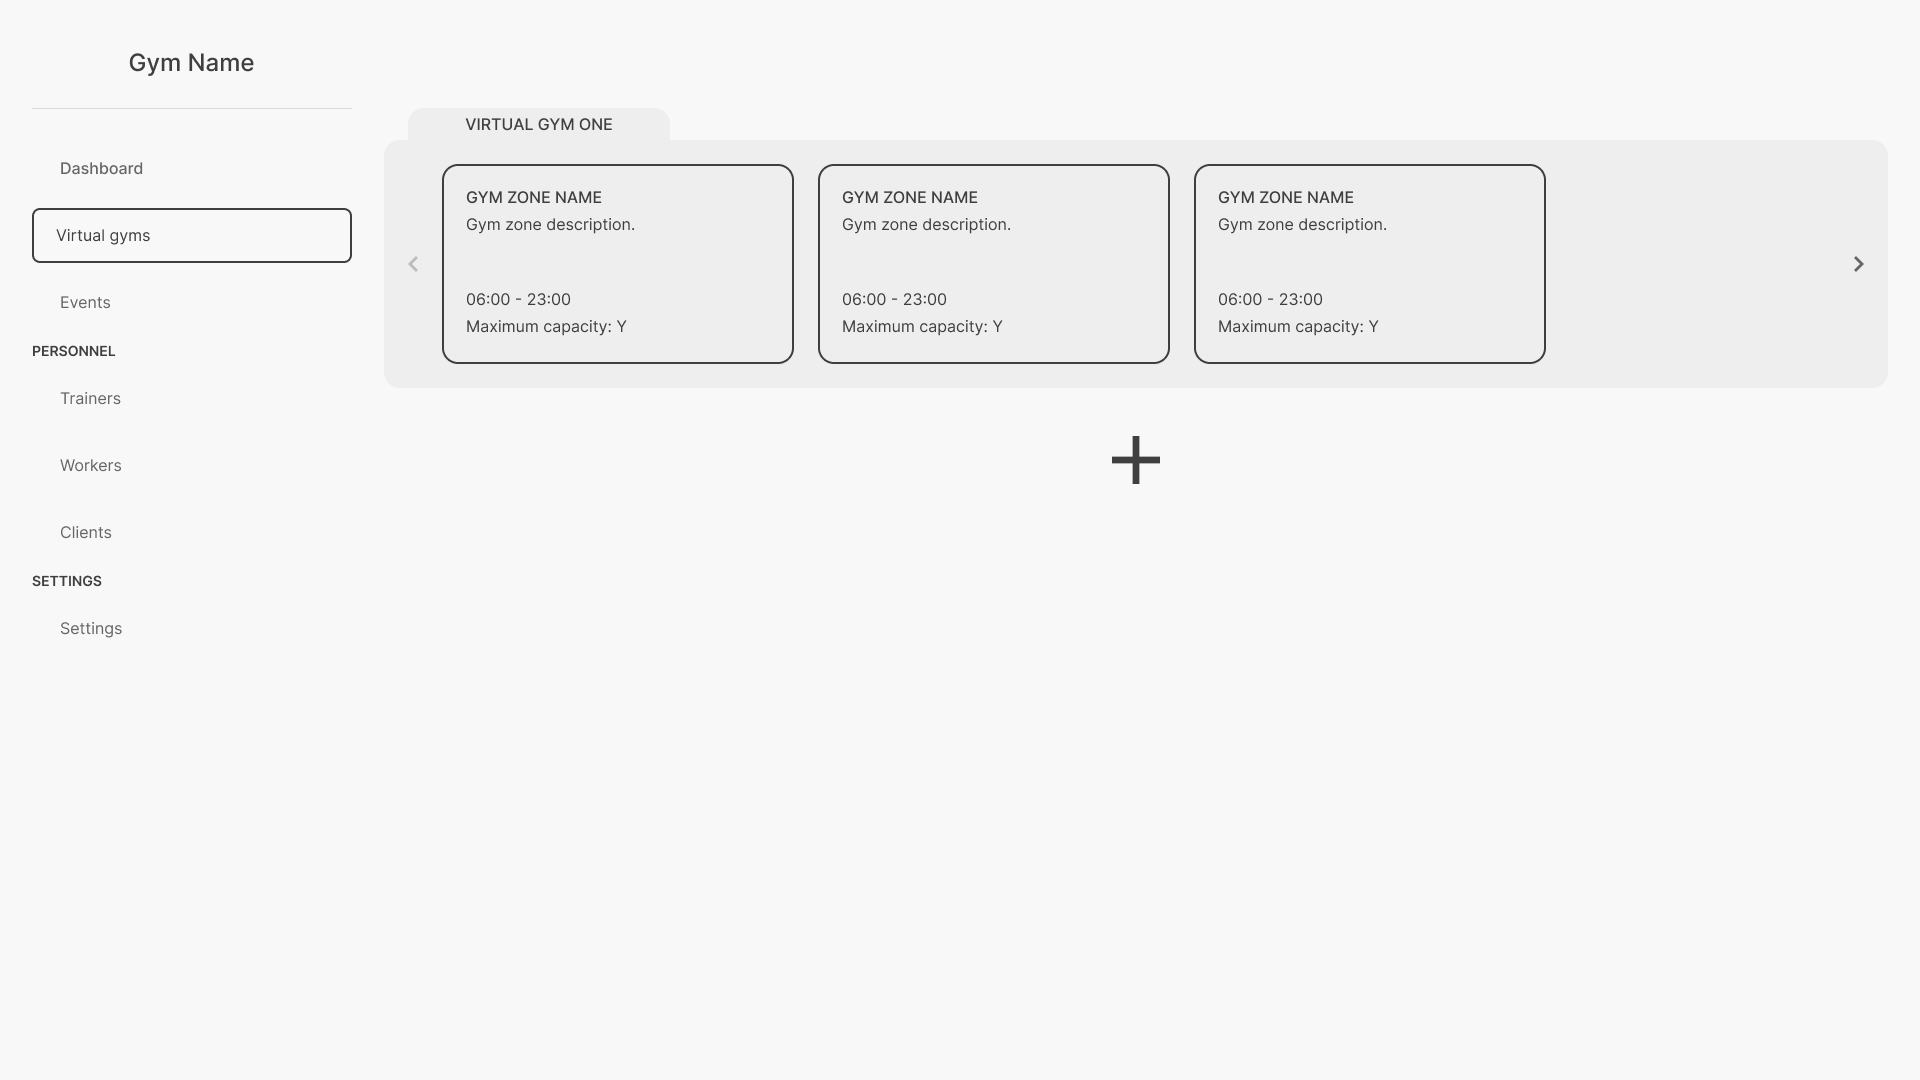
\includegraphics[width=\textwidth]{assets/ui/virtual-gyms.png}
	\caption{Virtual gym's page, which is accessed using the left navigation bar}
\end{figure}
\begin{figure}[H]
	\centering
	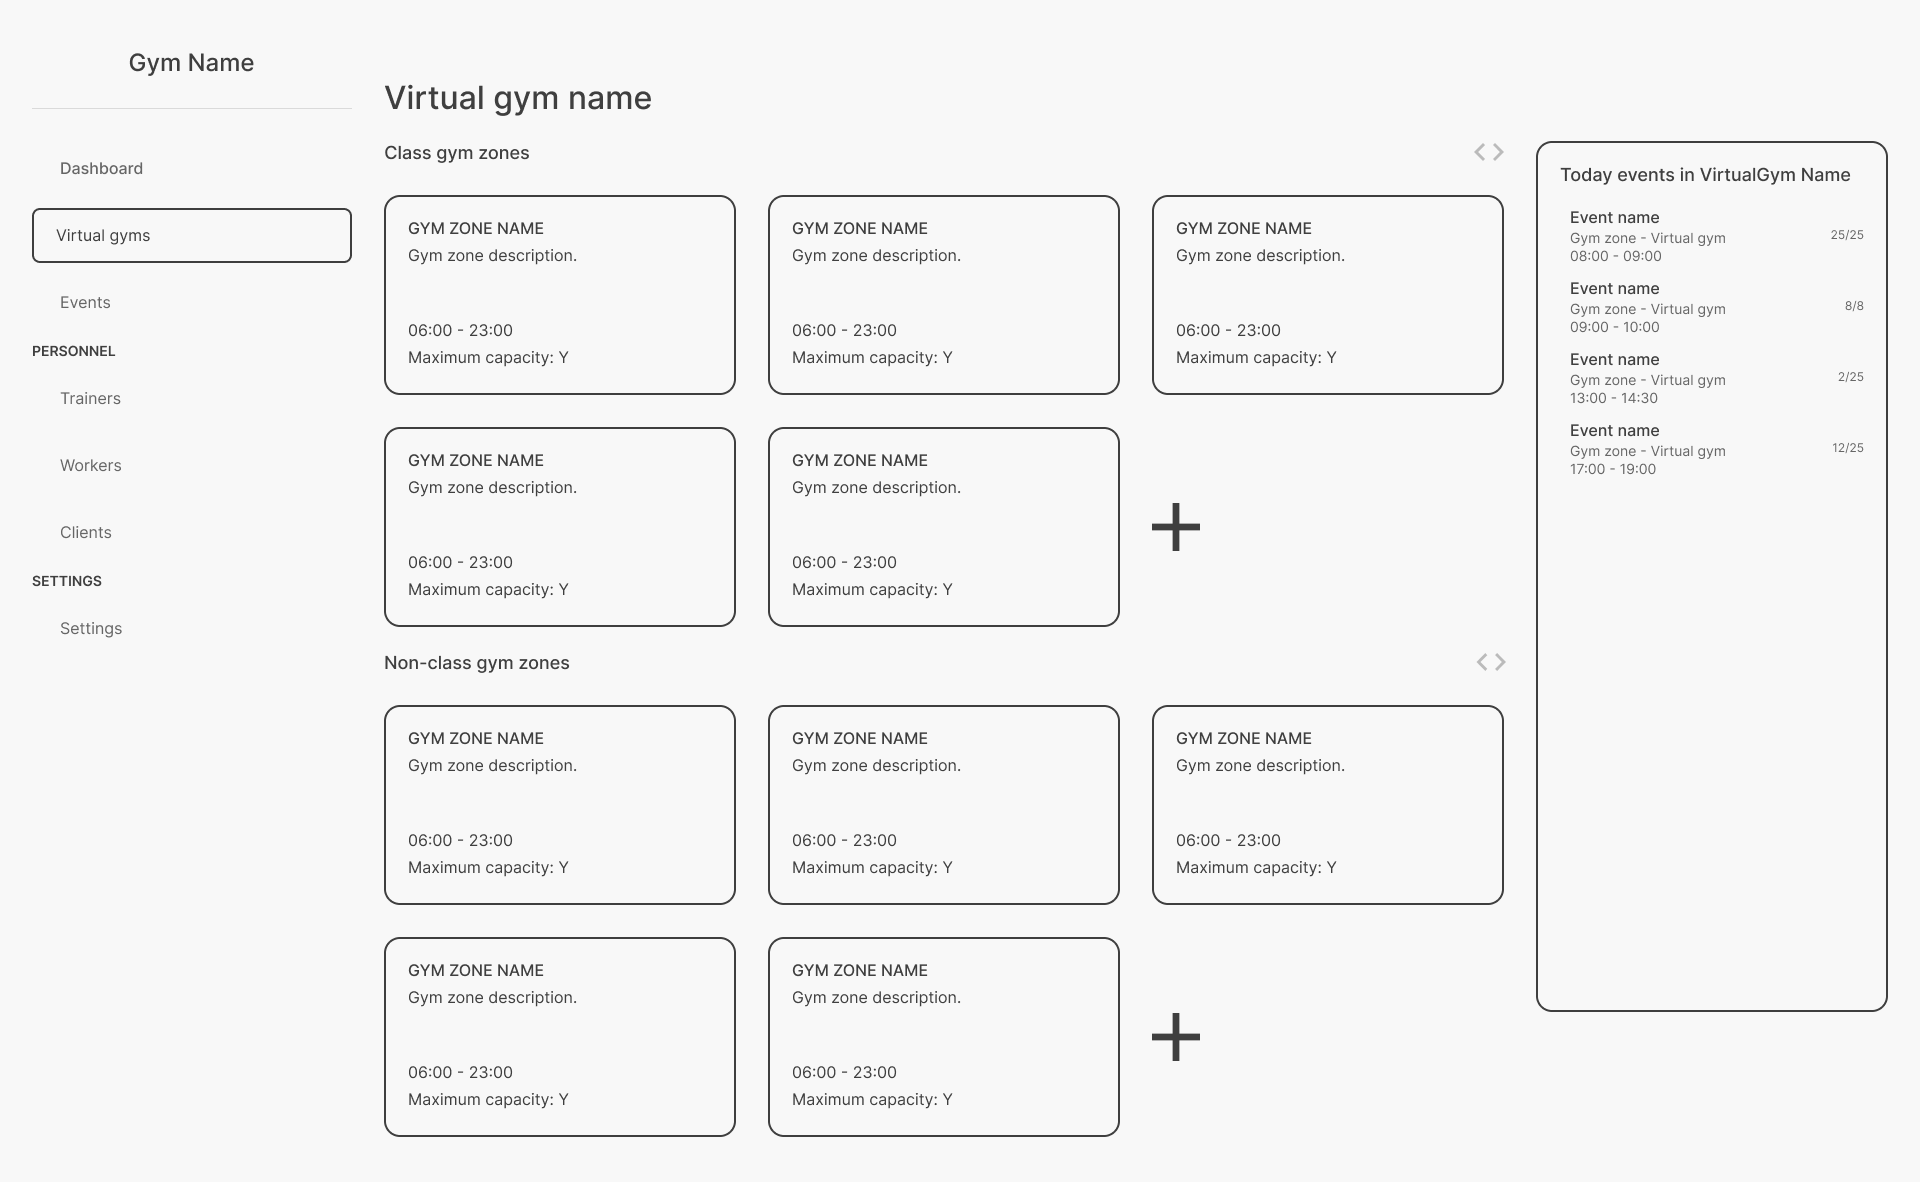
\includegraphics[width=\textwidth]{assets/ui/virtual-gym.png}
	\caption{Single virtual gym view, accessed by clicking on a virtual gym}
\end{figure}
\begin{figure}[H]
	\centering
	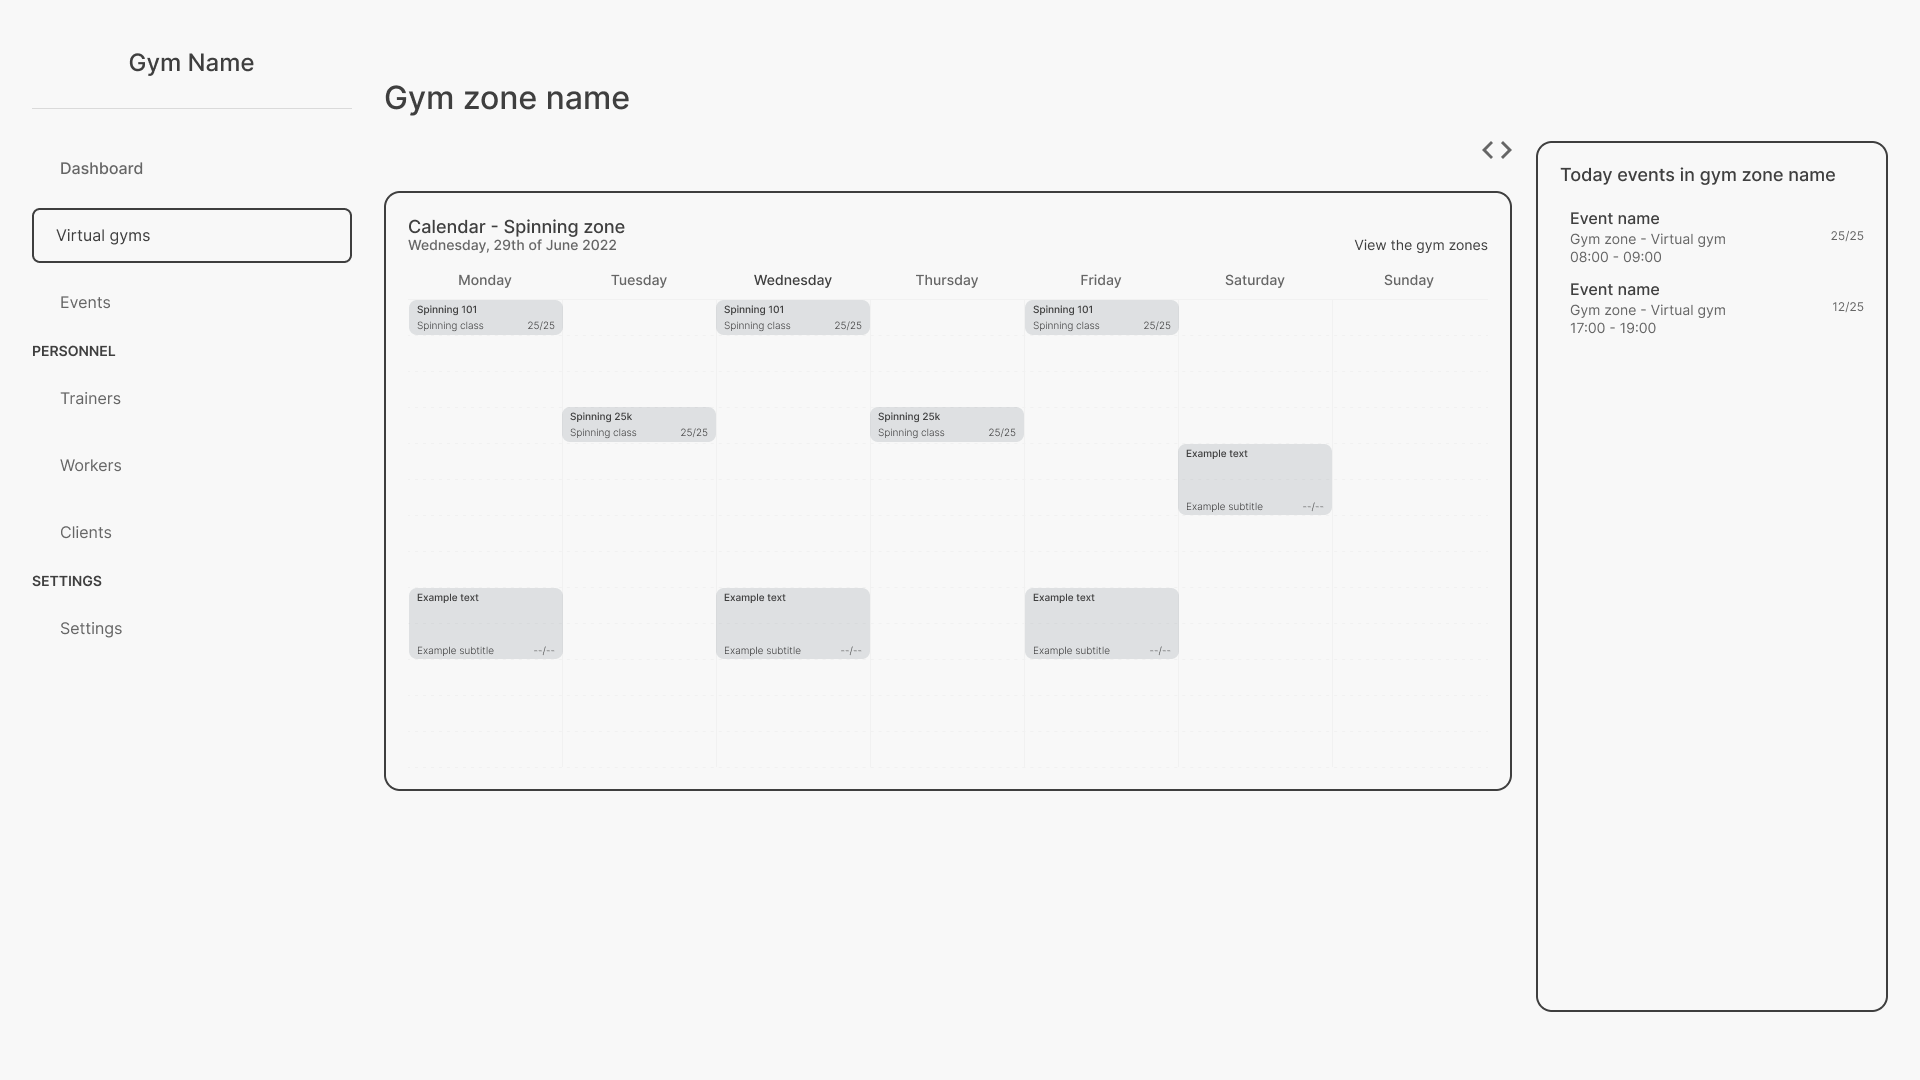
\includegraphics[width=\textwidth]{assets/ui/class-gym-zone.png}
	\caption{Class gym zone page, accessed by clicking on any class-type gym zone}
\end{figure}
\begin{figure}[H]
	\centering
	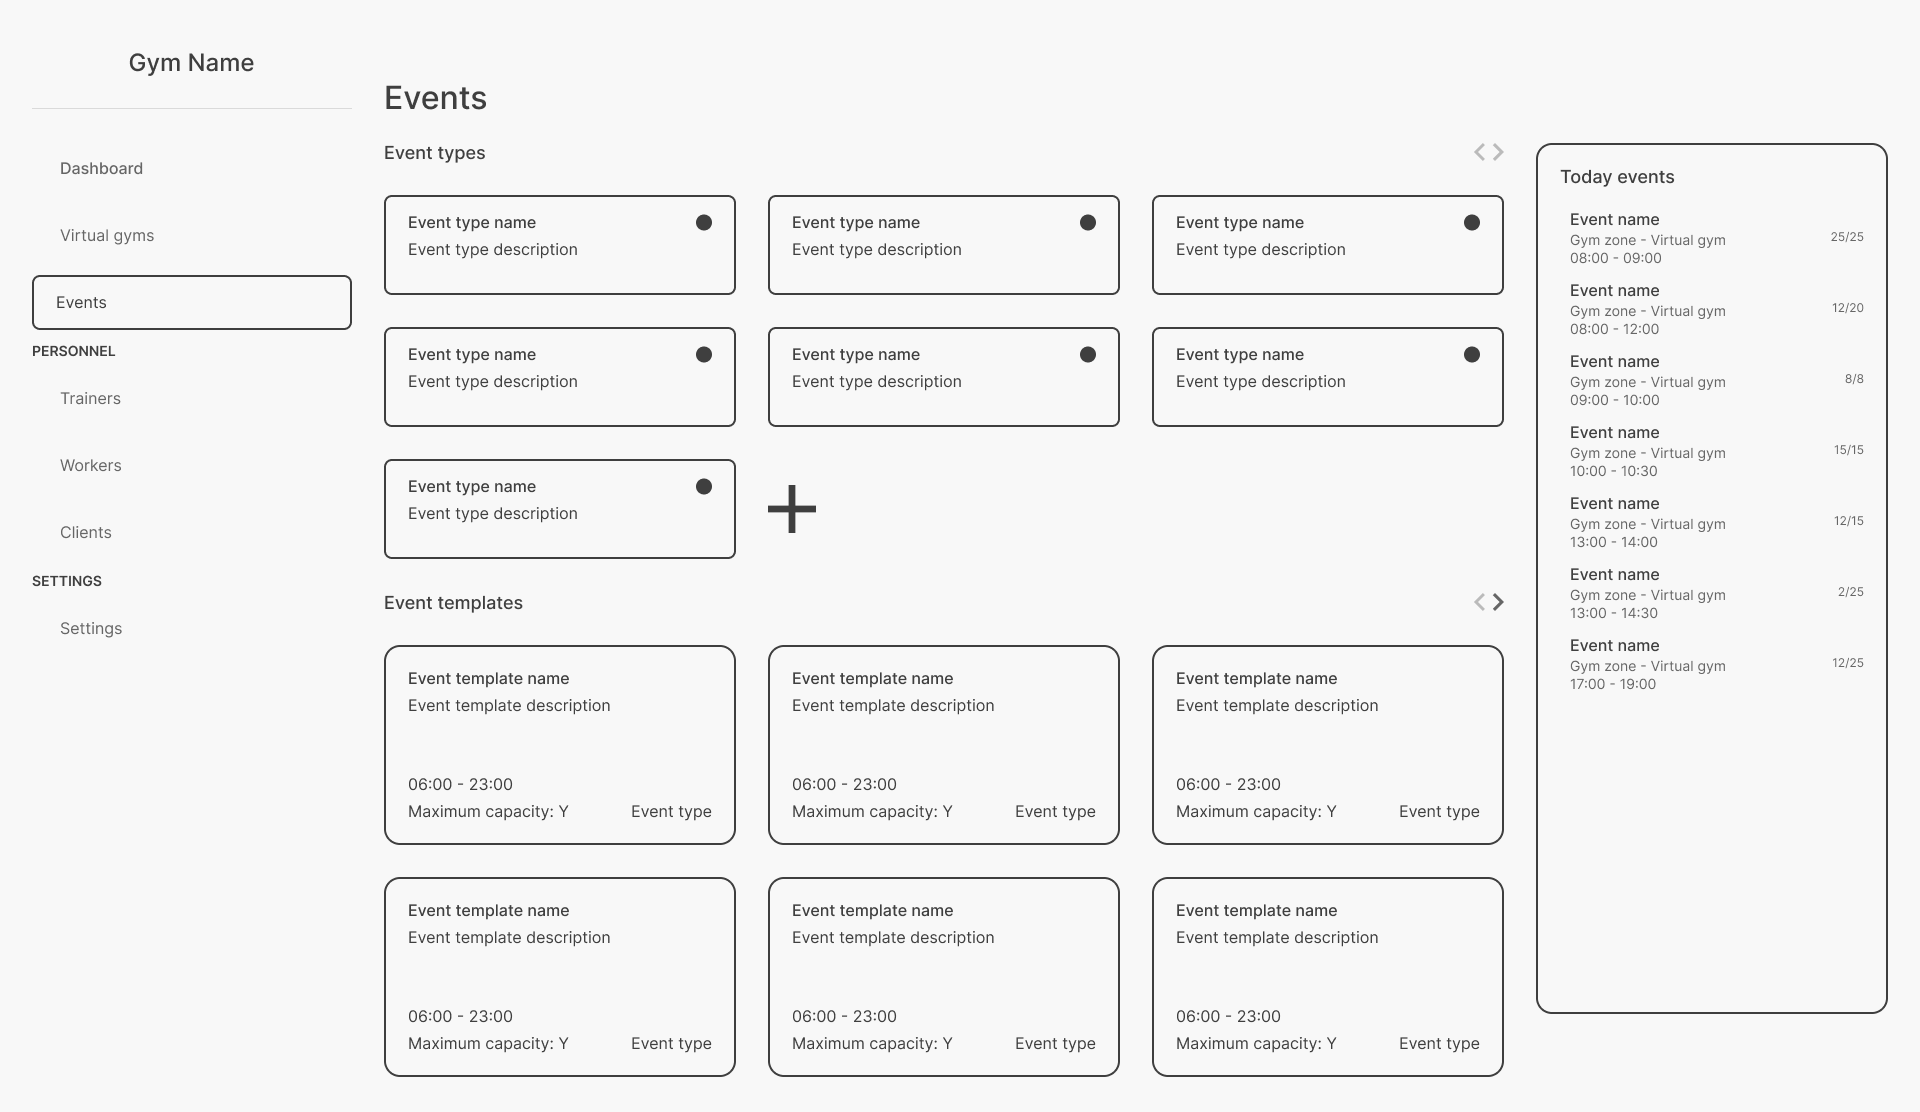
\includegraphics[width=\textwidth]{assets/ui/events.png}
	\caption{Event's page, which is accessed using the left navigation bar}
\end{figure}
\begin{figure}[H]
	\centering
	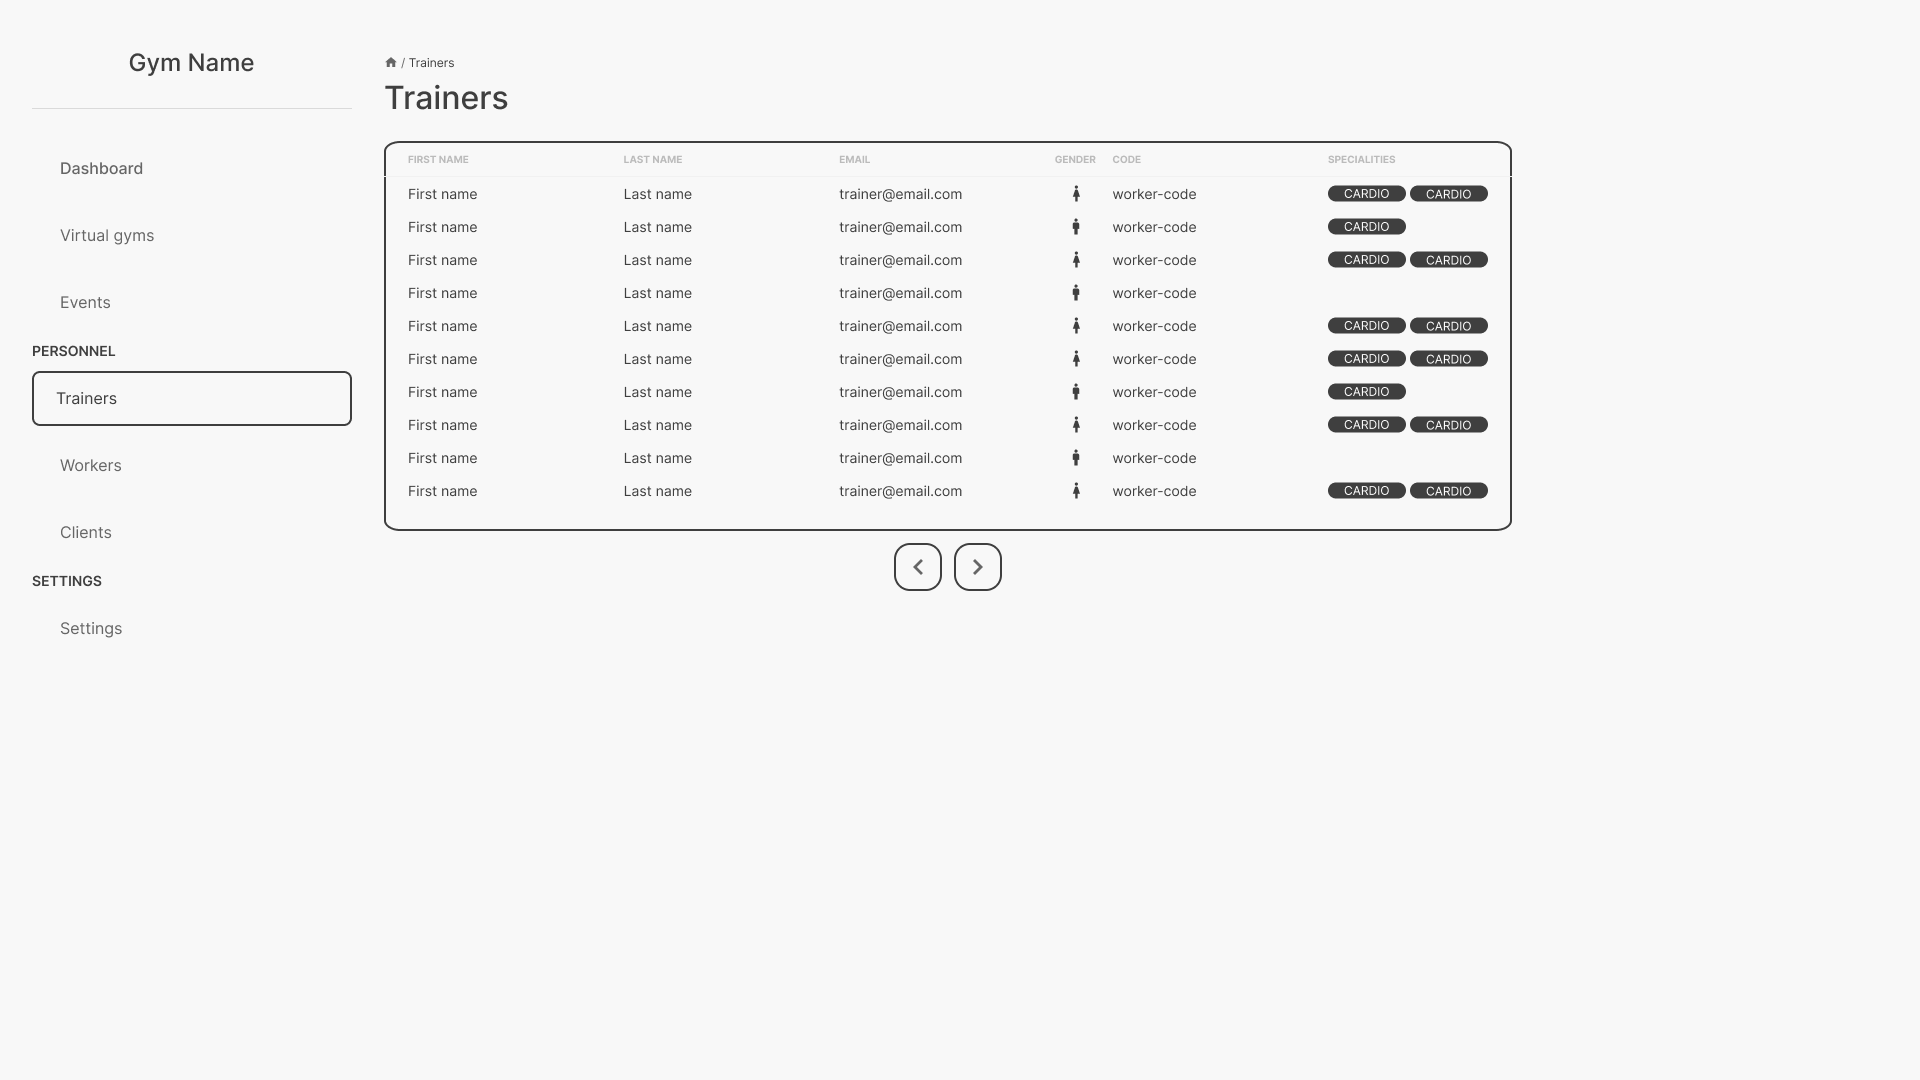
\includegraphics[width=\textwidth]{assets/ui/trainers.png}
	\caption{Trainer's page, which is accessed using the left navigation bar}
\end{figure}
\begin{figure}[H]
	\centering
	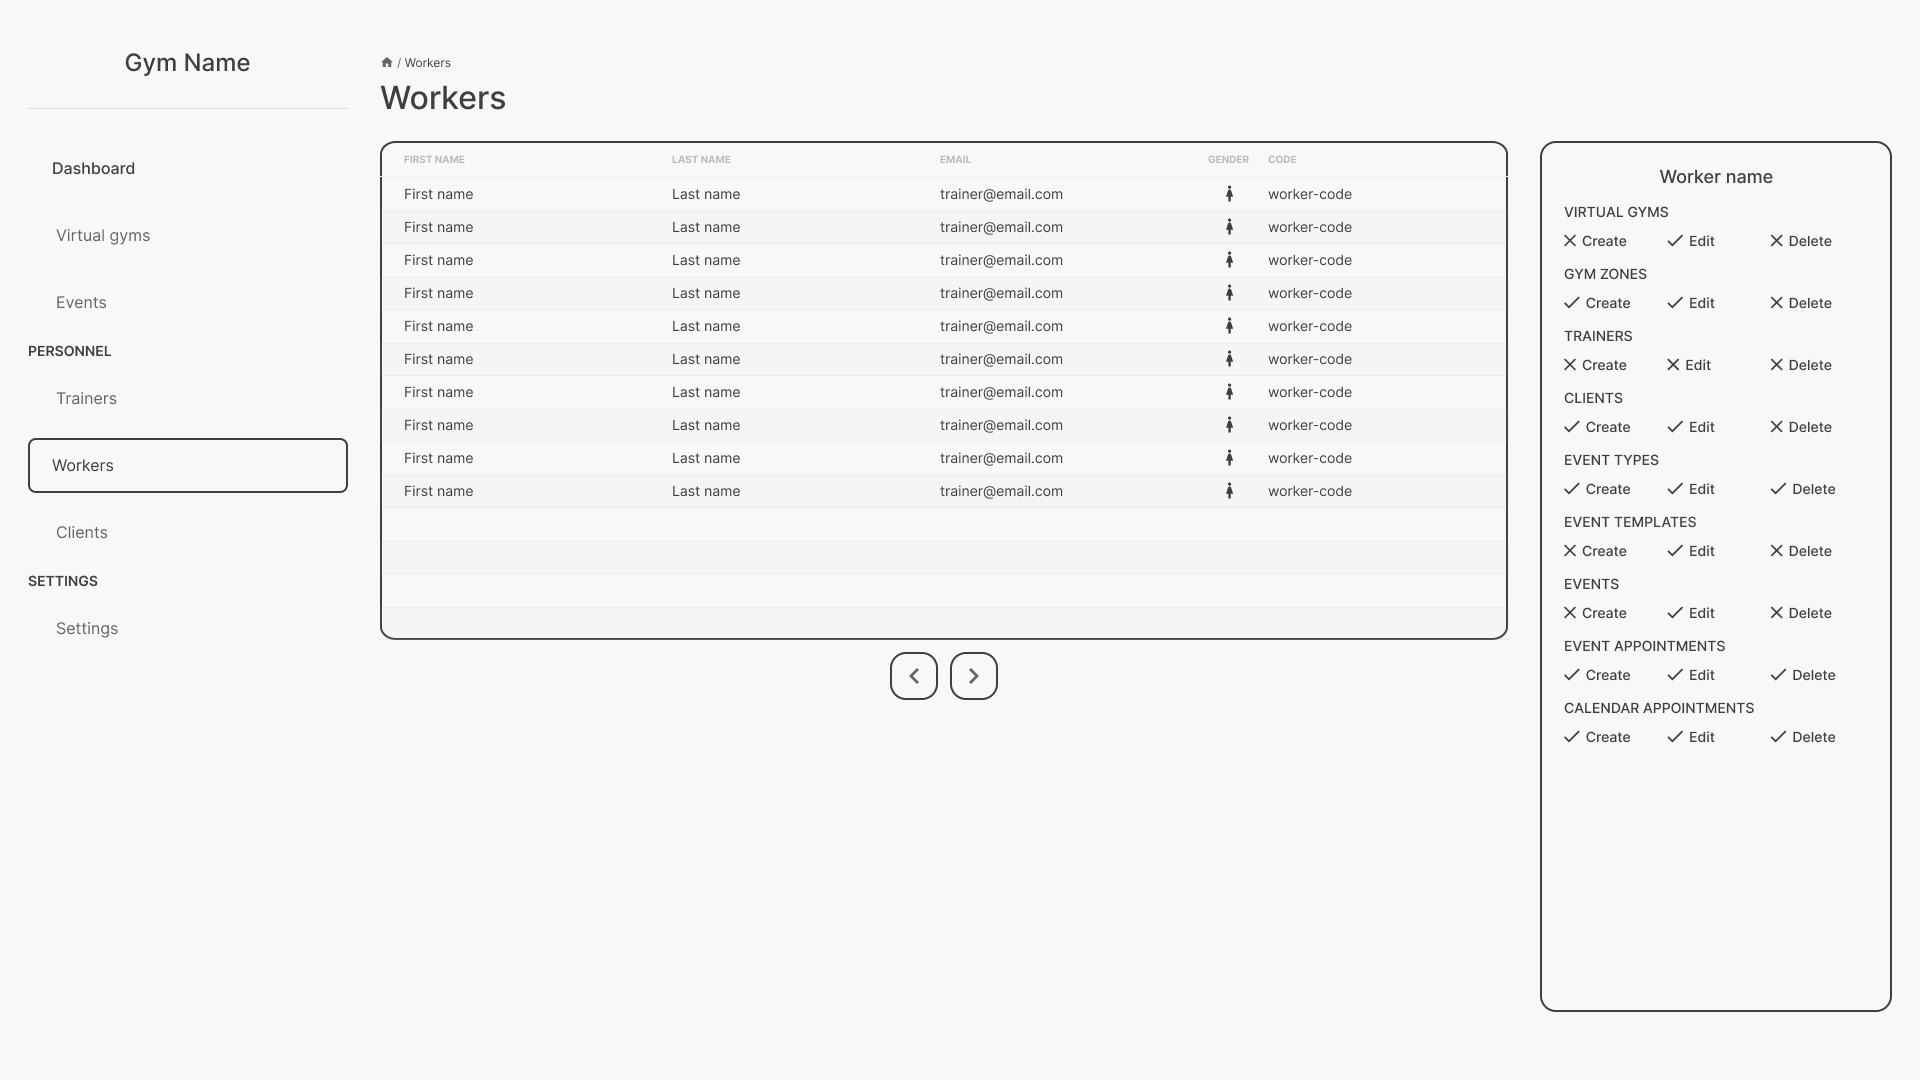
\includegraphics[width=\textwidth]{assets/ui/workers.png}
	\caption{Worker's page, which is accessed using the left navigation bar}
\end{figure}
\begin{figure}[H]
	\centering
	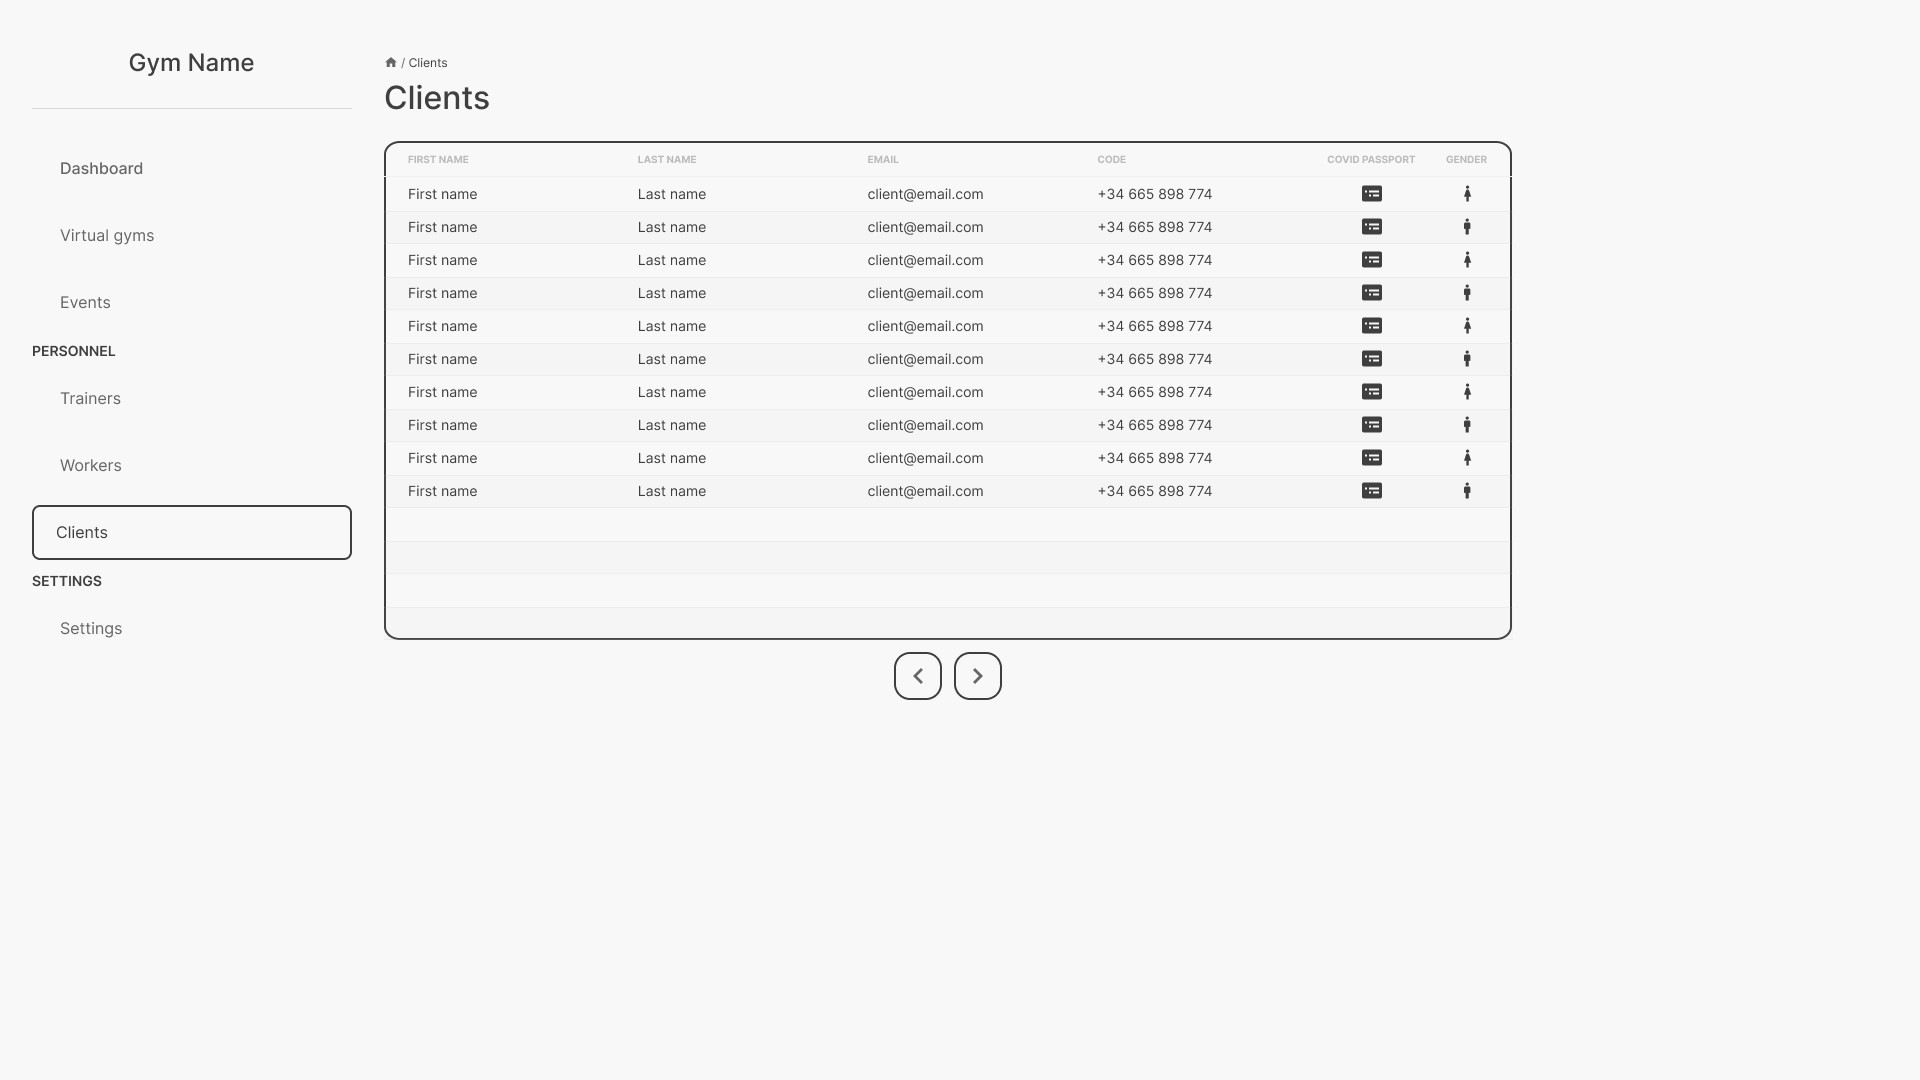
\includegraphics[width=\textwidth]{assets/ui/clients.png}
	\caption{Client's page, which is accessed using the left navigation bar}
\end{figure}
\begin{figure}[H]
	\centering
	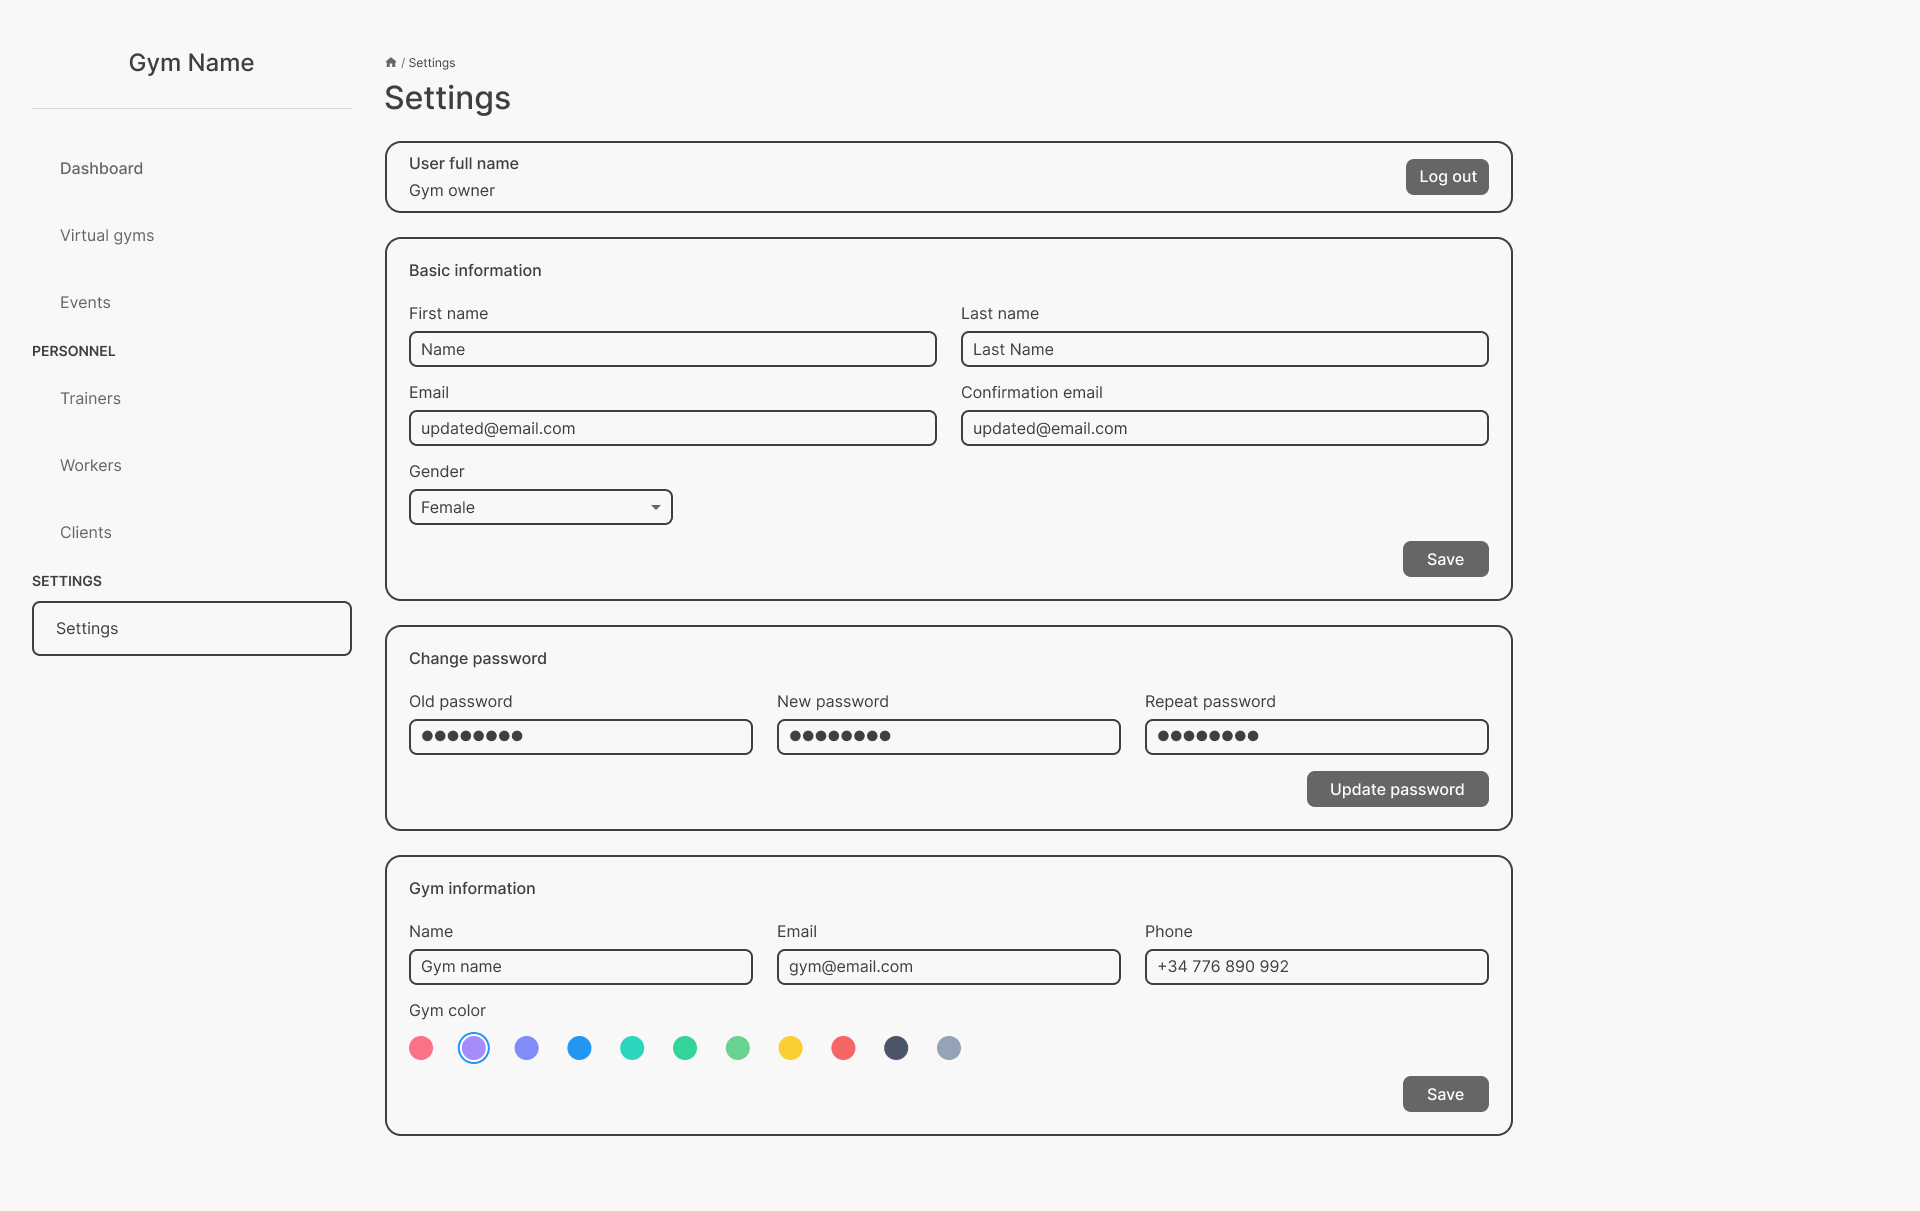
\includegraphics[width=\textwidth]{assets/ui/settings-owner.png}
	\caption{Settings page}
\end{figure}
% #endregion Images
\chapter{Implementation and trials}
\section{Introduction}
The goal of this chapter is to explain the development process, from the thinking of the application and its structure, to the actual development of it. It will also include and explanation of how the application has been constantly tested\footnote{Most testing involves unit and integration testing. In the API application, end-to-end testing has been implemented. For the UI applications, do not have end-to-end testing implemented due to a lack of time}.
\section{Organizing the idea}
When I came up with the idea for the application, I ended up with a mix of thoughts that had to be organized and connected. Therefore, the first step was to write an extensive explanation of the application, the goal of the application, what it would do and what it would not do, trying to cover as many details as I could. After revising and rethinking the idea, I ended up with a potential project that \emph{made sense} and could provide value to future clients.
\\[8pt]
Once the application had been described, defining the functionalities of such were easier. However, I needed to define a possible structure for such application. It was then when I decided to develop three applications: the landing page, the core application and the client application. I found interesting to distinguish between the client and the core application in order to simplify the development process. Mostly, when an application is expected to cover the most amount of possibilities and users, it ends which an enourmous amounts of checks and even repeated code. Knowing so, I decided to split it in two applications, while at the same time reducing the amount of boilerplate code. Knowing the existence of Nx, I had the logistic problem of maintaining a monorepo with the applications and libraries solved by such tool.
\\[8pt]
Even though it would probably change in structure, the initial idea of the architecture was there, and from it, I could start specifying the functional and non-functional requirements. It was probably the most time demanding task of the project, alongside structuring the working packages. Now that such parts were defined, I was able to visualise a roadmap for the development of the system.
\section{Application development}
I started developing the API application as it helped to define the database. It ended up being the most repetitive project to develop as there are many endpoints which are quite similar, however others were such a challenge, as involved complex queries. Once the server had been ``finished''\footnote{It is hard to consider a project finished, as product applications need constant improvements and changes in order to keep up with the market.}, I started designing the user interface. knowing available endpoints of the server helped with the thingking of the UI, yet at the same time it helped me realise what was lacking in the server. Therefore, after having finished the design, I got back to the API, adding what was mssing and cleaning up the code\footnote{Such thing was also expected in the roadmap, as it was my intention to revise the server after designing the UI.}.
\\[8pt]
The next step was to start developing the UI applications. The core application had the most amount of logic and difficulty, which is the reason why I started with such project. I knew I would have to add a lot of components and views which would later be reused in the client application. This is the reason why the working packages for the core application have more estimated time than the client application. With Nx has been extremely easy and simple to abstract common code and keep it in the shared libraries, which can be easily used and referenced in any application. If in the future it is needed to add another application, the development process would be extremely simple, since most components could be reused.
\\[8pt]
Since then, I have been developing most of the core application. When most of it had been finished, I started developing the client application. With it, I had to start abstracting some of the code that was in the core application, so that it can be reused.
\\[8pt]
Finally, I have also tracked the time that I have spent in each task, using Jira's smart commits. However, I started tracking the time spent at the end of December 2021, meaning that the overall spent time is 100\% accurate. Furthermore, it also contains the time that I have spent develoing the applications, without counting the time spent with documentation. The following table contains the time spent with the task types and their priority:
\\[8pt]
One of the things to note about this table is the fact that not much time has been spent with \emph{bug} type tasks. It storngly believe it is due the fact that I have been testing the code constantly.
\subsection{Continuous integration}
One of the things that I explained in previous sections was the importance of having continuous integration, which would help to know if the code developed would cause errors or not. Also, with integration tests, it would be easier to verify if the component or controller work as expected. It was also one of the reasons why I chose Nx as a build tool, as it allows you to test for a specific project.
\\[8pt]
Knowing so, I defined multiple workflows \cite{github-workflows} which would run if there were changes in the different project directiories\footnote{GitHub worflows allow you to trigger worflows on changes made in a given folder path.}. The worflows would be run in two conditions:
\begin{enumerate}
	\item If there is a push in the \texttt{develop} branch.
	\item If a pull request if opened.
\end{enumerate}
The development process would be:
\begin{enumerate}
	\item Creating a branch with the name of the Jira issue. Using such naming convention, when accessing an issue in Jira, it was easier to find the issue branches.
	\item Adding as many changes as wanted, while also adding tests. If the changes were added in the API application, it should include unit, integration and e2e tests. If the changes where added in any library of any UI application, it should include unit and integration tests.
	\item Once the task has been finished, a PR should be created which would trigger the workflows.
	\item If all checks pass, the PR can be merged into the wanted branch.
\end{enumerate}
Using the PRs, it becomes really easy to identify issues, and it ensures that not a single line of coded is merged without knowing it does not pass its tests. As an addition to the checks, I also integrated CodeCov, which is a freemium tool that helps to visualise the coverage of the project\footnote{The CodeCov configuration file can be found in the \texttt{codecov.yaml} in the root folder of the repository.}. The CodeCov integration adds a comment to the pull request summarizing the changes made and how such changes modify the coverage of the project.
\begin{figure}[H]
	\centering
	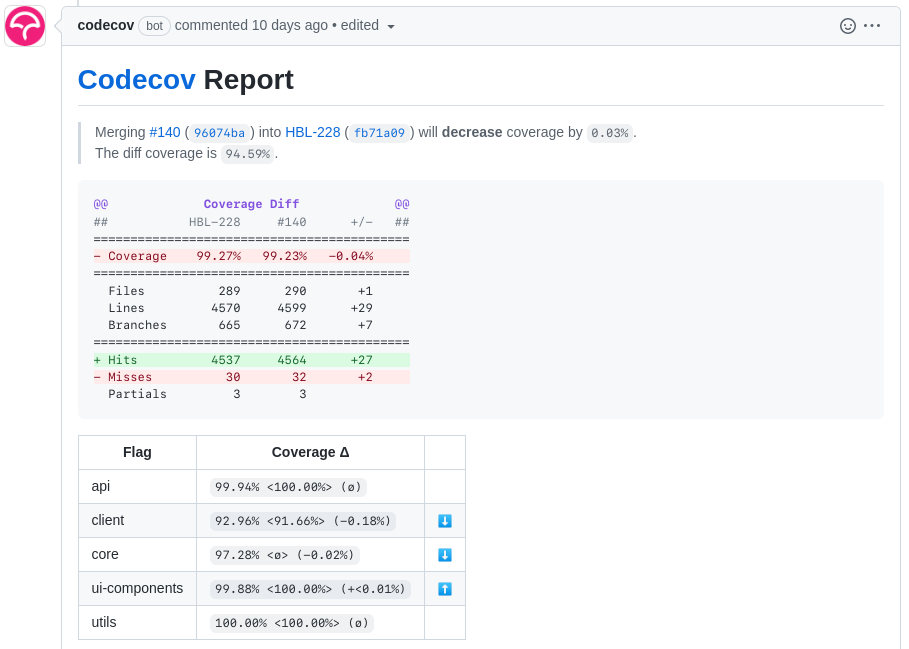
\includegraphics[width=\textwidth]{assets/codecov-example.png}
	\caption{Example of the comment generated by the CodeCov command}
\end{figure}
As explained before, the API server runs an e2e test. Such test requires a fake database and also takes more time to initialise, run and finish. Therefore, the end-to-end tests are not run on every merge to develop or every PR, but when the code is merged to the \texttt{main} branch. The end-to-end test starts a docker container in the GitHub action that will contain the database which will be used by the tests.
\section{Trials}
Aside from the implemented tests, the UI application has been manually tested in order to find bugs that may not have been covered by the automated tests. In the case of the API, testing the endpoints has been a bit harder, yet the Postman software has been used in order to test the endpoints. In case of the UI applications, they have been tested by finding edge cases when running the appliation.
\\[8pt]
When a bug has been found, I firstly checked the tests to see why it was not being covered or if it was a bug in the test, as it is something that can happen. If the bug was found in the tests, I updated the tests and later fixed the actual code. If not, I would search the bug in the code, to later cover it with the tests.
\chapter{Deployment and results}
\section{Deployment}
The deployment of the application would be the latest step once the 3 applications have been fineshed. Once again, due to the lack of time, I have not been able to finish all the features I had in mind before the application is deployed. Nevertheless, the current product is enough to be shown to potential clients, meaning that if I found any gym or company interested in such product, with what has been developed, I ensure it would be enough to attract them to the app.
\\[8pt]
Aside from that, a mind map of how the applications would work for the public, would be by accessing them from a public URL. The applications would be running in a cloud service, AWS to name one, and most likely deployed as docker images, which would fasten the deployment and it would be easier to automate. However, due to lack of time and money, the application has not been deployed, meaning it can not be accessed from any device, other than the local machine. In order to run the application from the local machine, the installation manual can be found in the code repositiry, as well as in the documentation for each application, in the repository aswell.
\section{Results}
There are some views that did not fit in the screen, therefore two images have been made. Furthermore, most of the create and update actions are performed inside a modal or a dialog. Instead of adding two screenshots with the same content, only with small text changed, only the create dialog has been attached. Furthermore, the zoom applied is of 90\%, allowing more content to be displayed in the screenshot.
\subsection{Core application}
In order to reduce the amount of screenshots that are added, the screenshots have been made when a user is logged as an owner. A worker's is nearly as the worker's one, just with some actions not allowed, depending on their permissions.
\subsubsection{Authentication}
\begin{figure}[H]
	\centering
	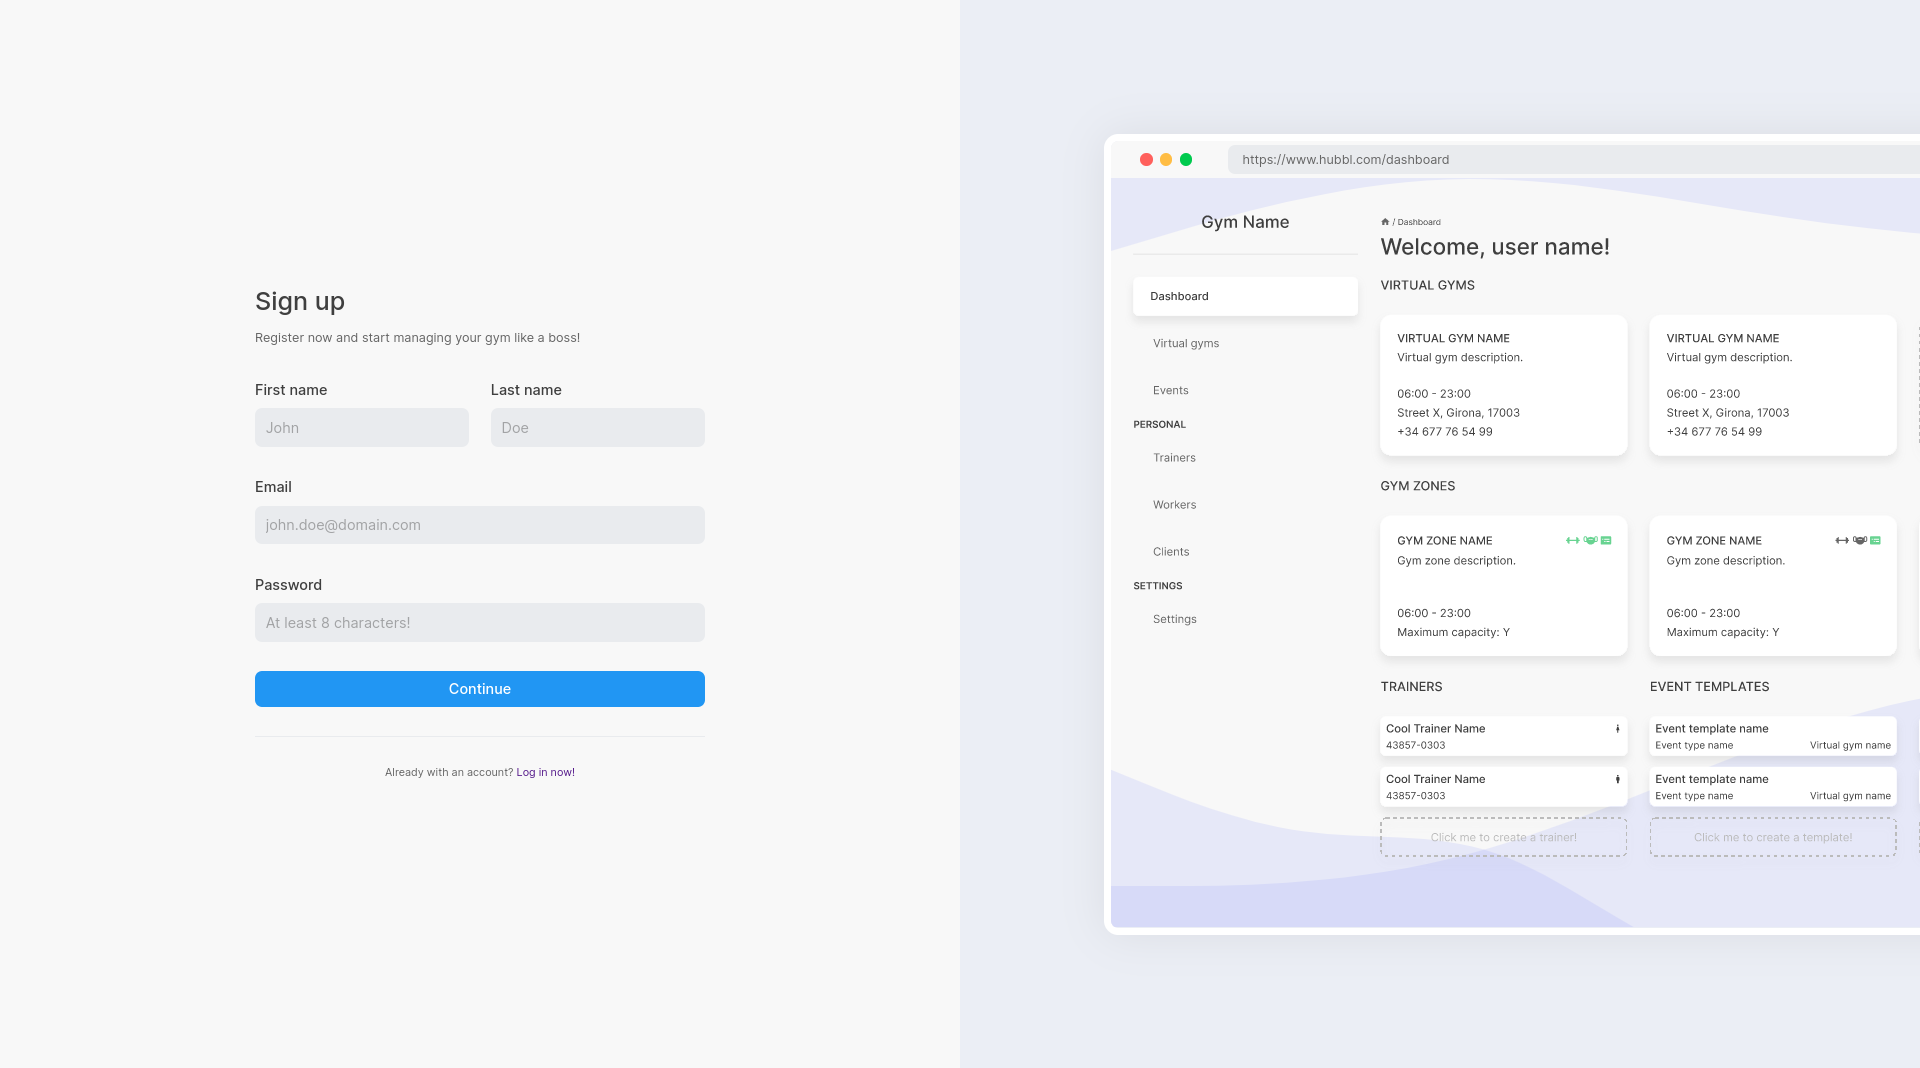
\includegraphics[width=\textwidth]{assets/core-screenshots/sign-up-one.png}
	\caption{Step one of the sign up process}
\end{figure}
\begin{figure}[H]
	\centering
	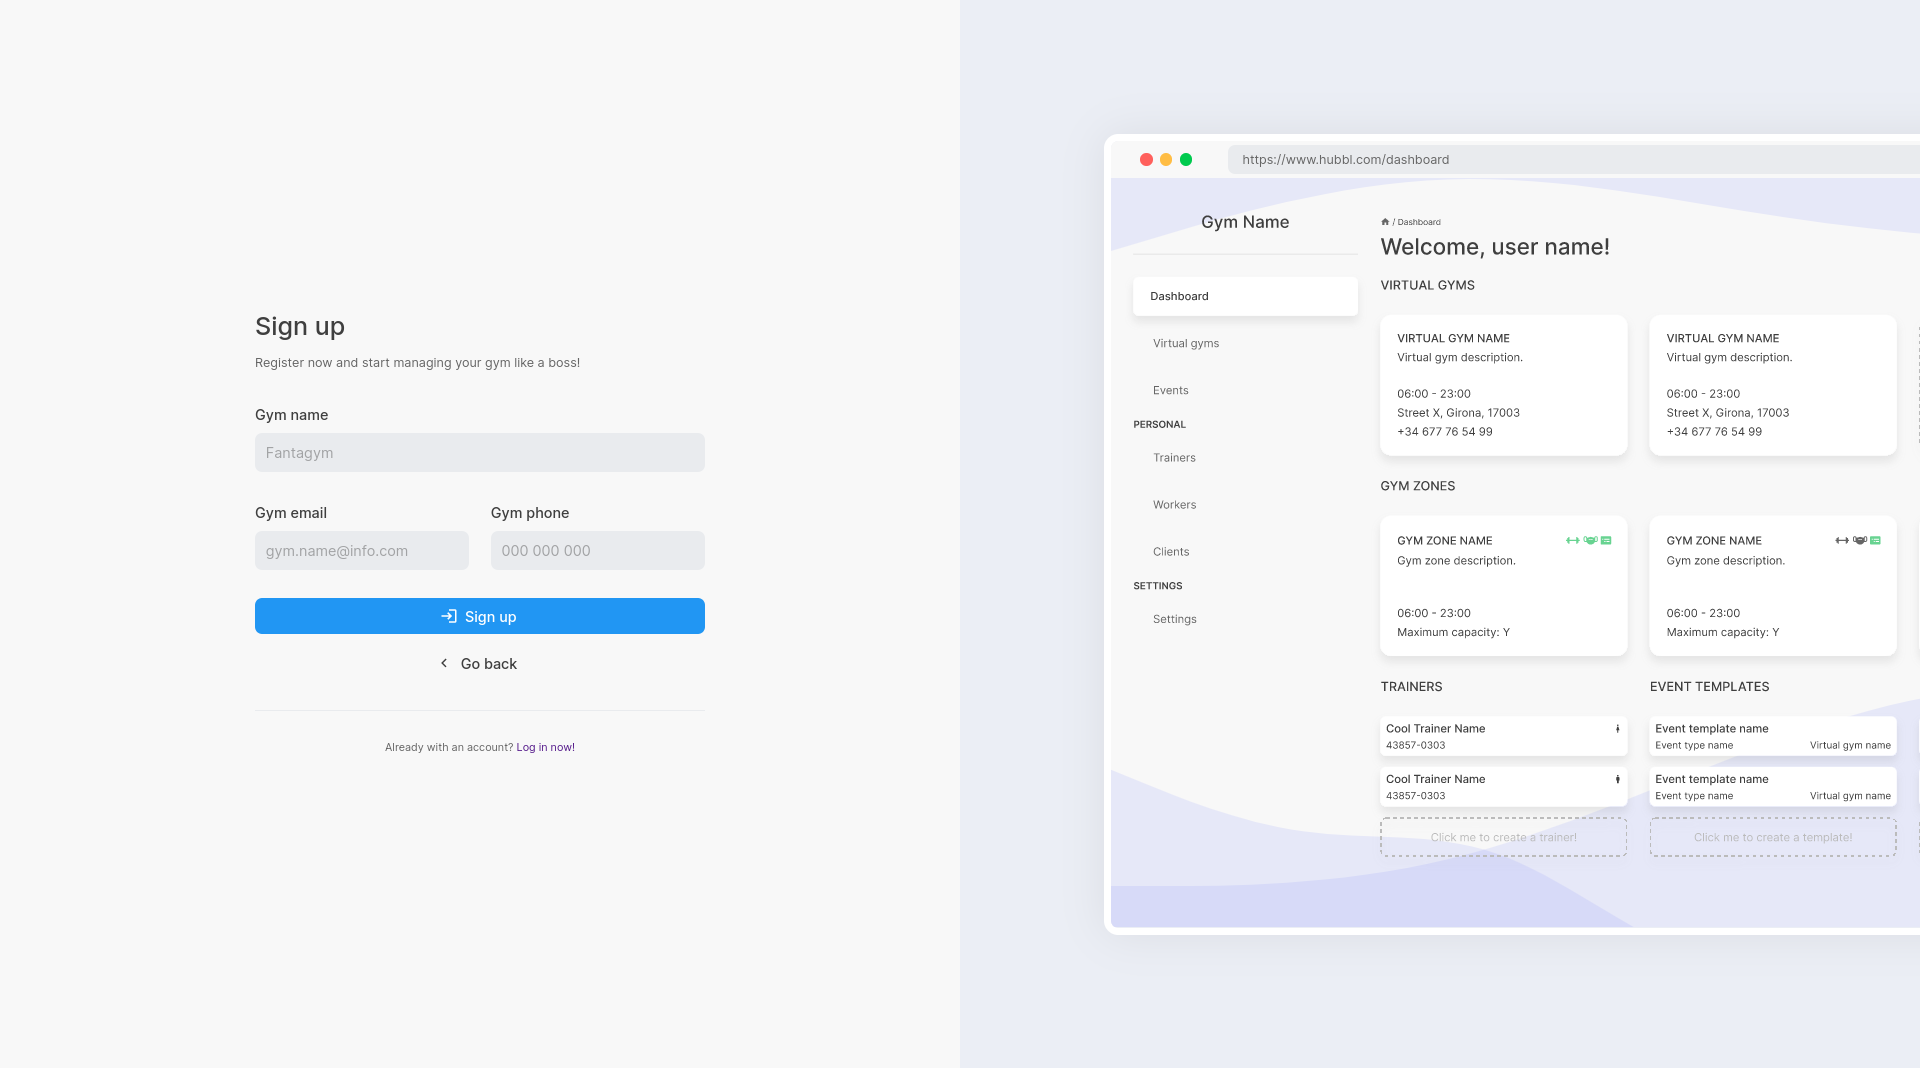
\includegraphics[width=\textwidth]{assets/core-screenshots/sign-up-two.png}
	\caption{Step two of the sign up process}
\end{figure}
\begin{figure}[H]
	\centering
	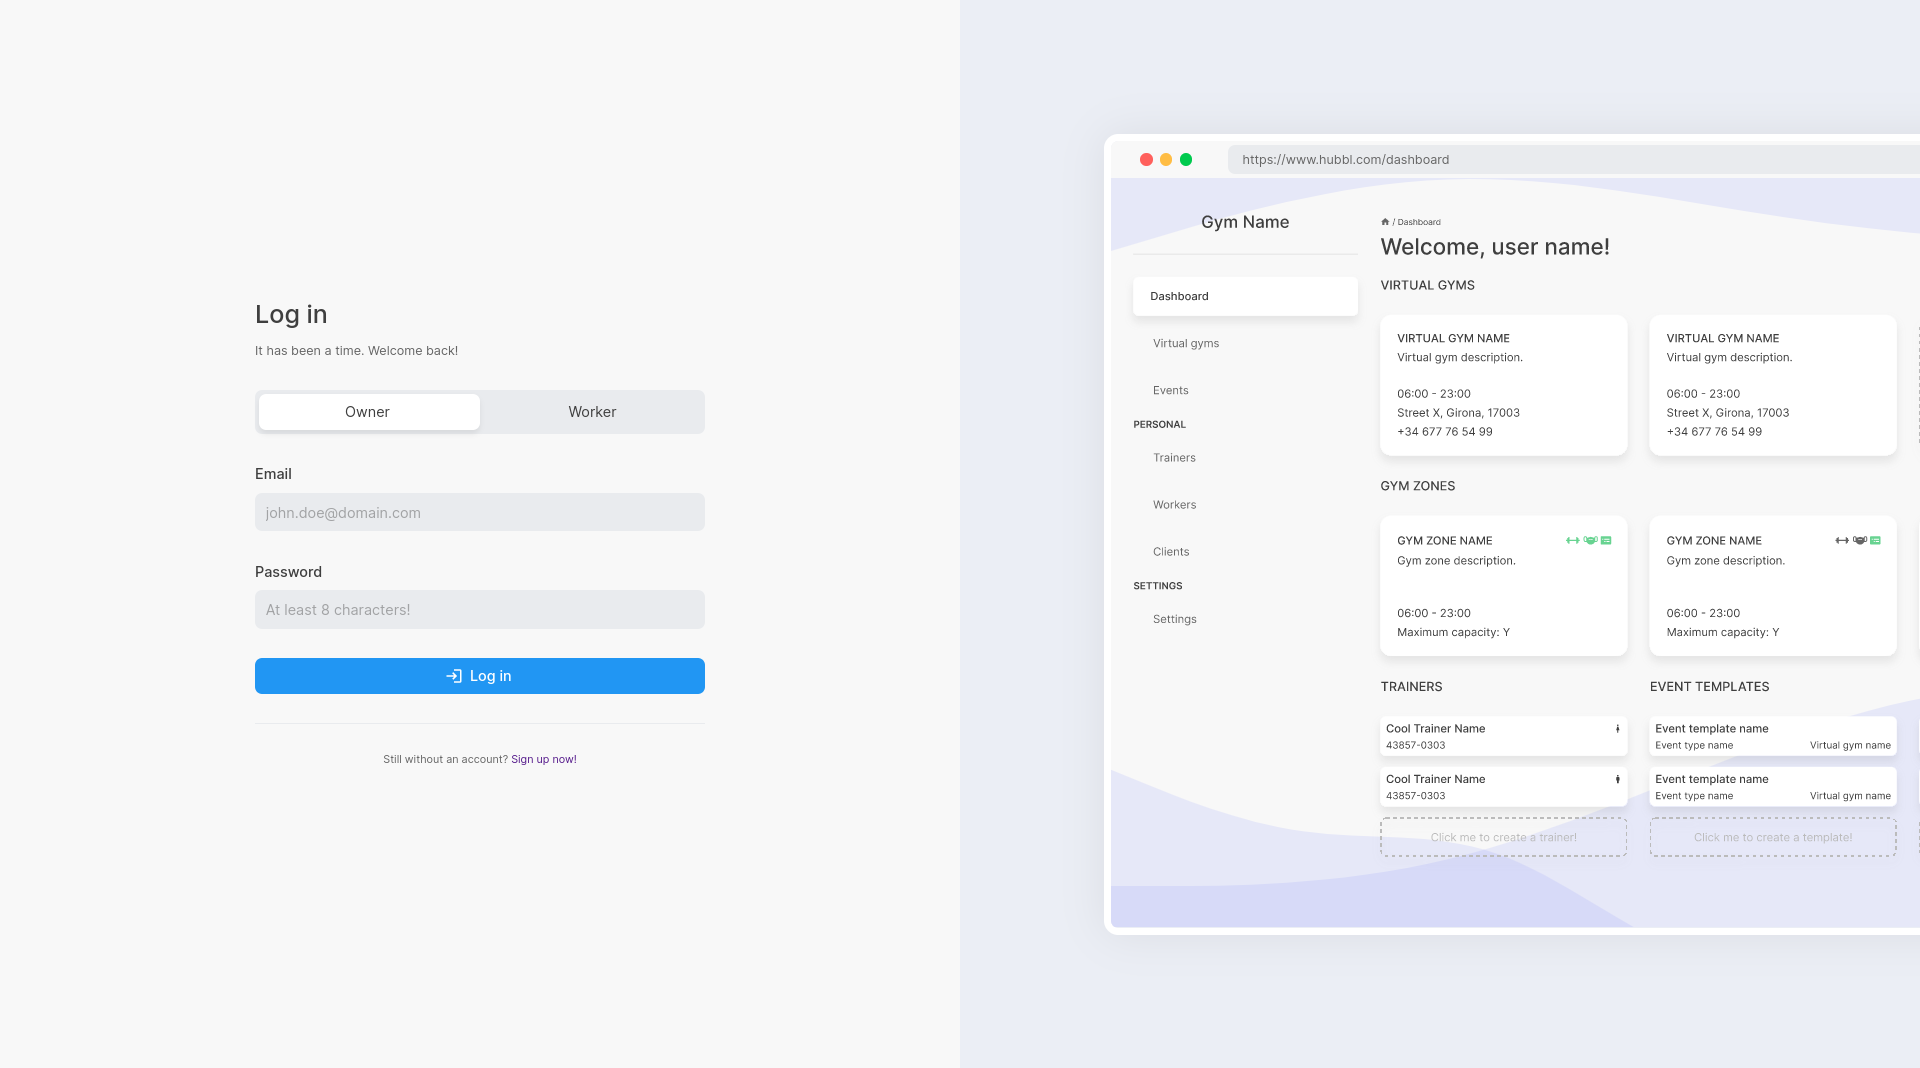
\includegraphics[width=\textwidth]{assets/core-screenshots/log-in.png}
	\caption{Log in page}
\end{figure}
\subsubsection{Dashboard page}
\begin{figure}[H]
	\centering
	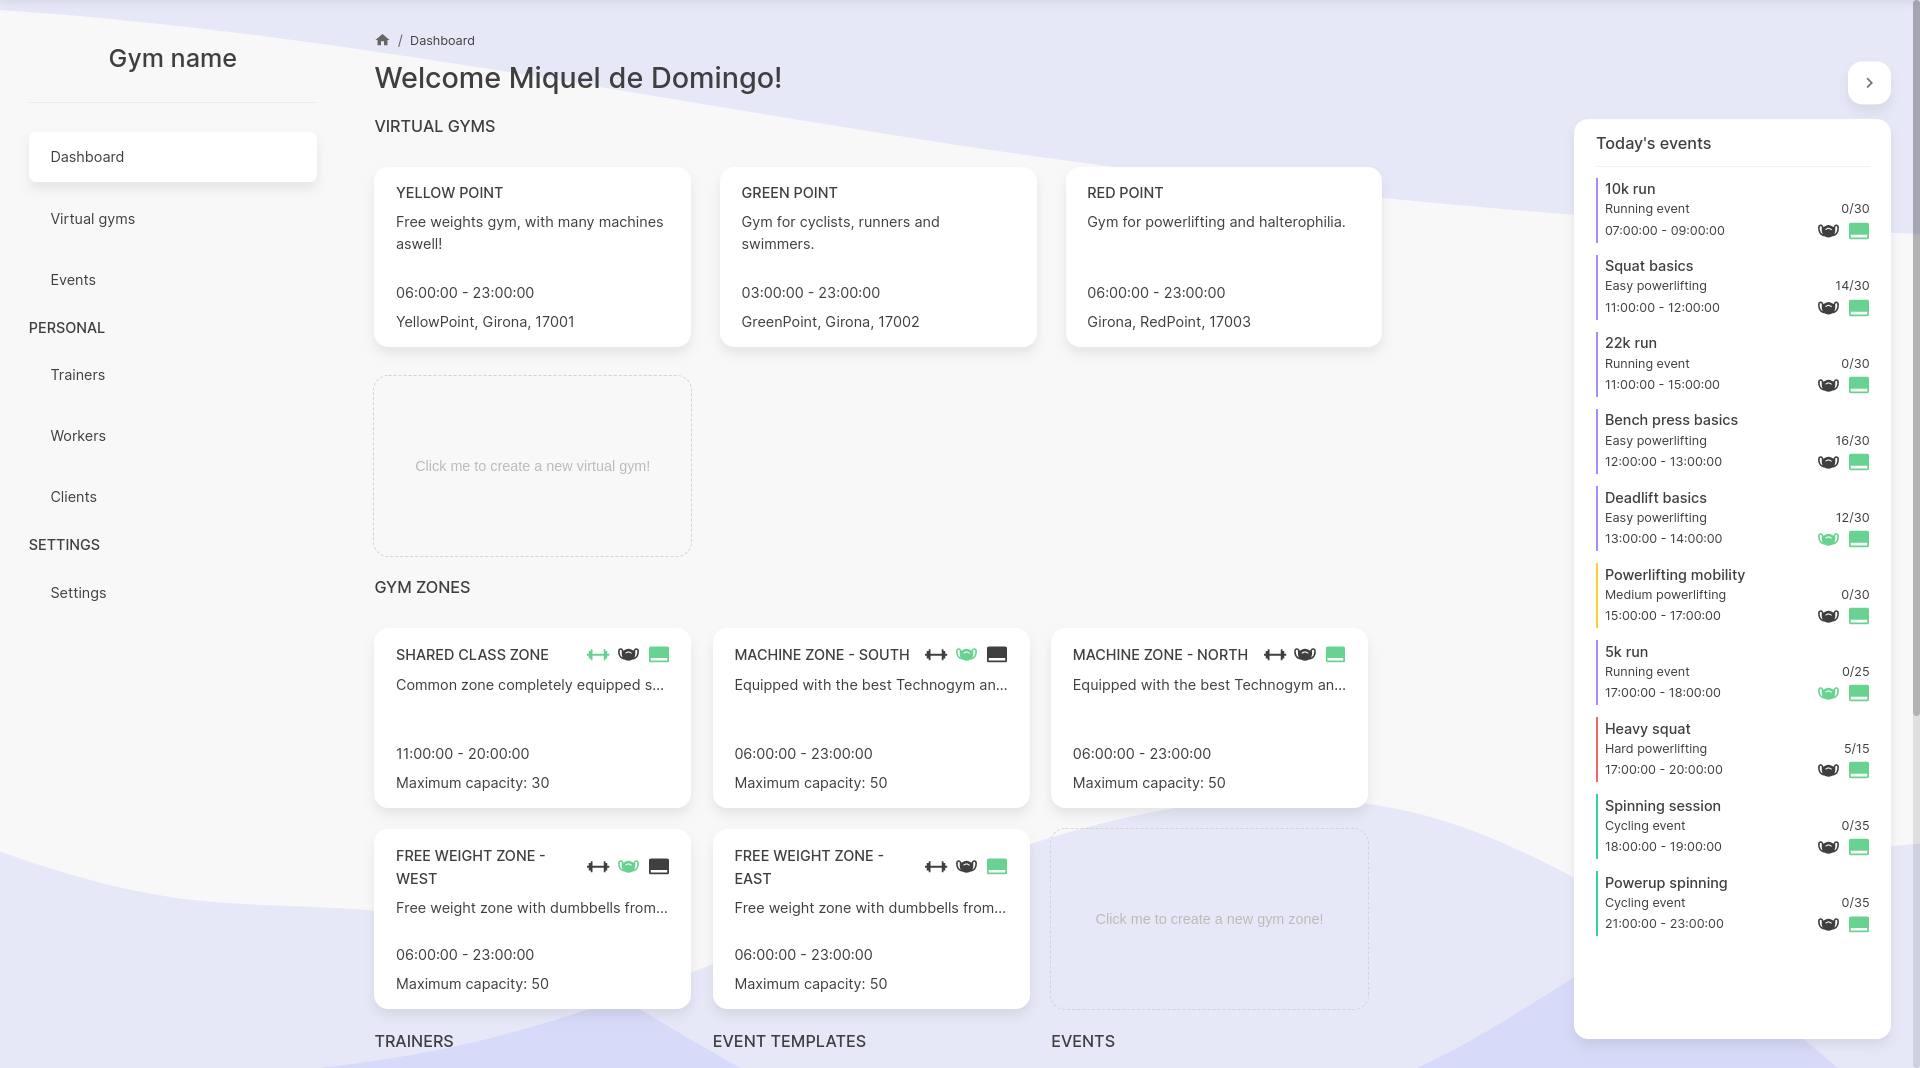
\includegraphics[width=\textwidth]{assets/core-screenshots/dashboard-one.png}
	\caption{First screenshot of the dashboard page}
\end{figure}
\begin{figure}[H]
	\centering
	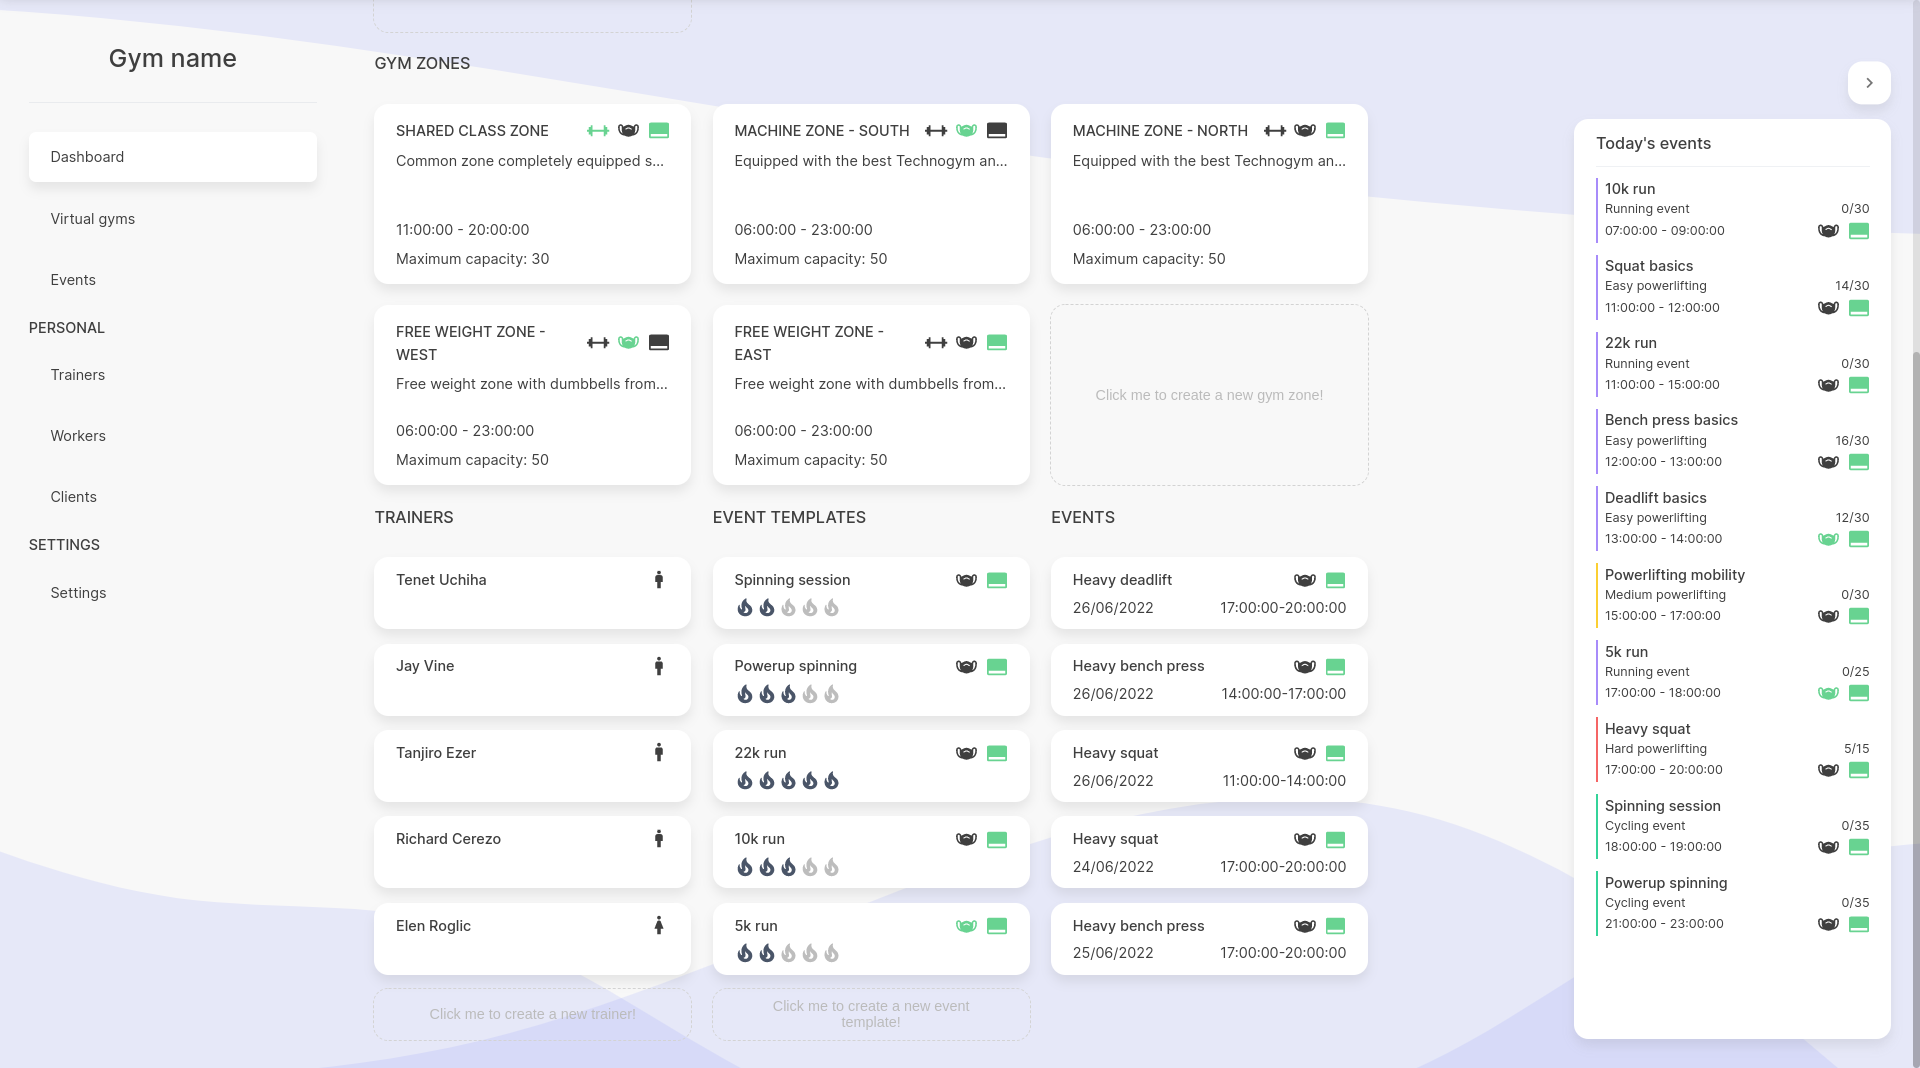
\includegraphics[width=\textwidth]{assets/core-screenshots/dashboard-two.png}
	\caption{Second screenshot of the dashboard page}
\end{figure}
\subsubsection{Virtual gyms}
\begin{figure}[H]
	\centering
	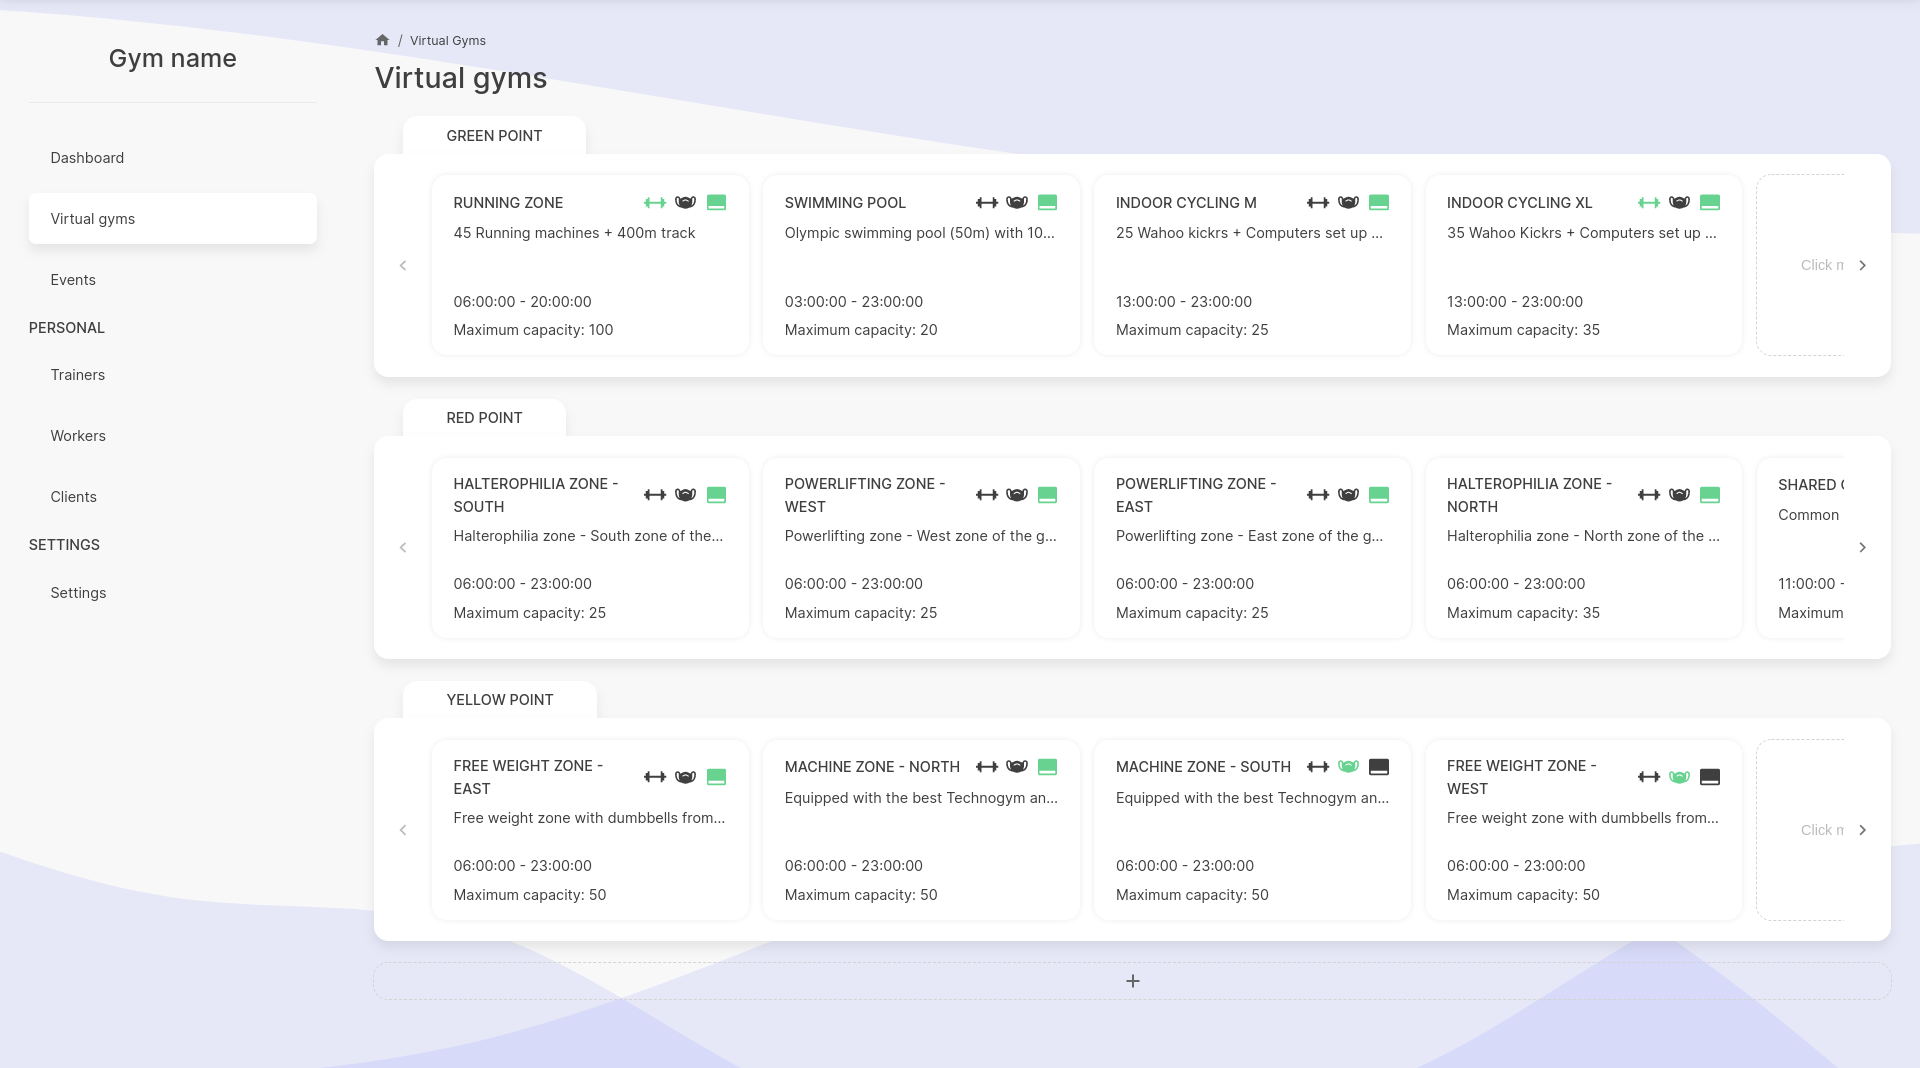
\includegraphics[width=\textwidth]{assets/core-screenshots/virtual-gyms.png}
	\caption{Virtual gyms page}
\end{figure}
Whenever a virtual gym has been clicked (by clicking at its name), the user is redirected to the above page, which displays all the gym zones of the chosen virtual gym.
\begin{figure}[H]
	\centering
	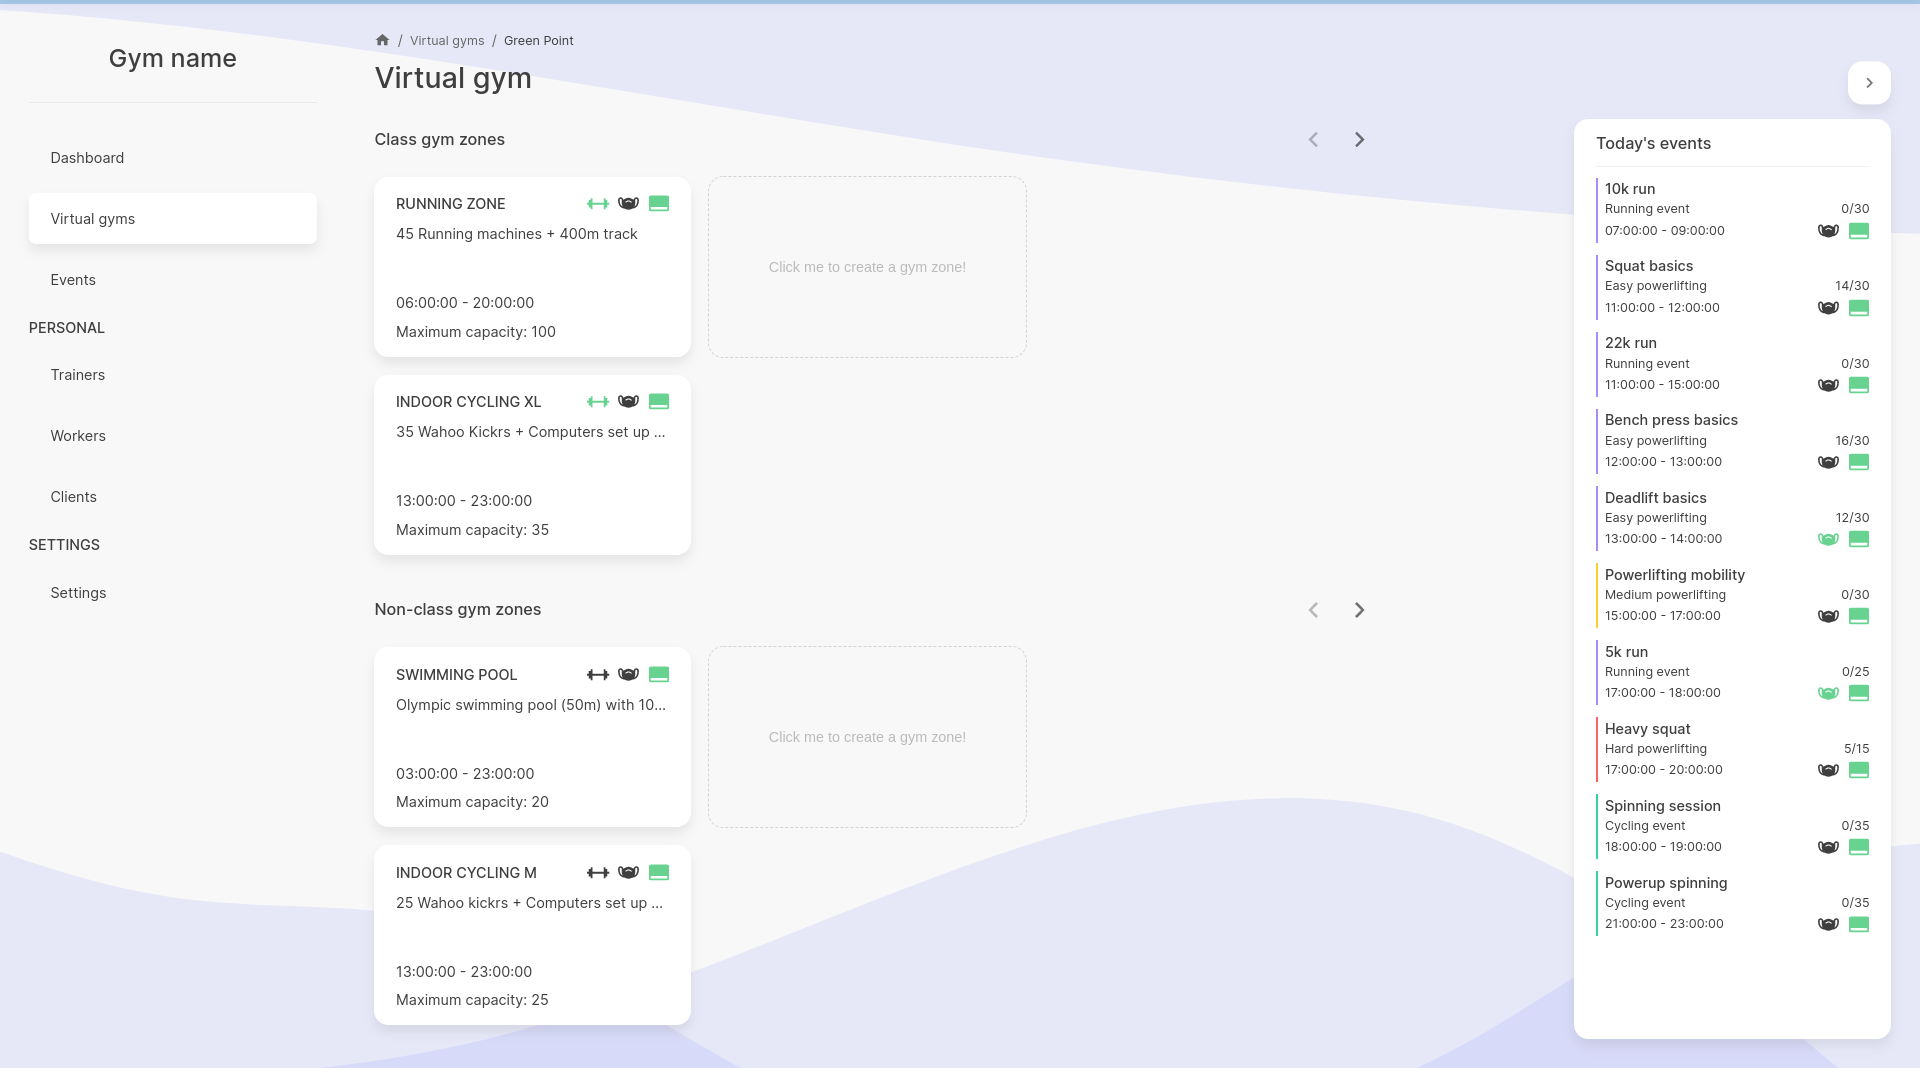
\includegraphics[width=\textwidth]{assets/core-screenshots/virtual-gym.png}
	\caption{Virtual gym page}
\end{figure}
\begin{figure}[H]
	\centering
	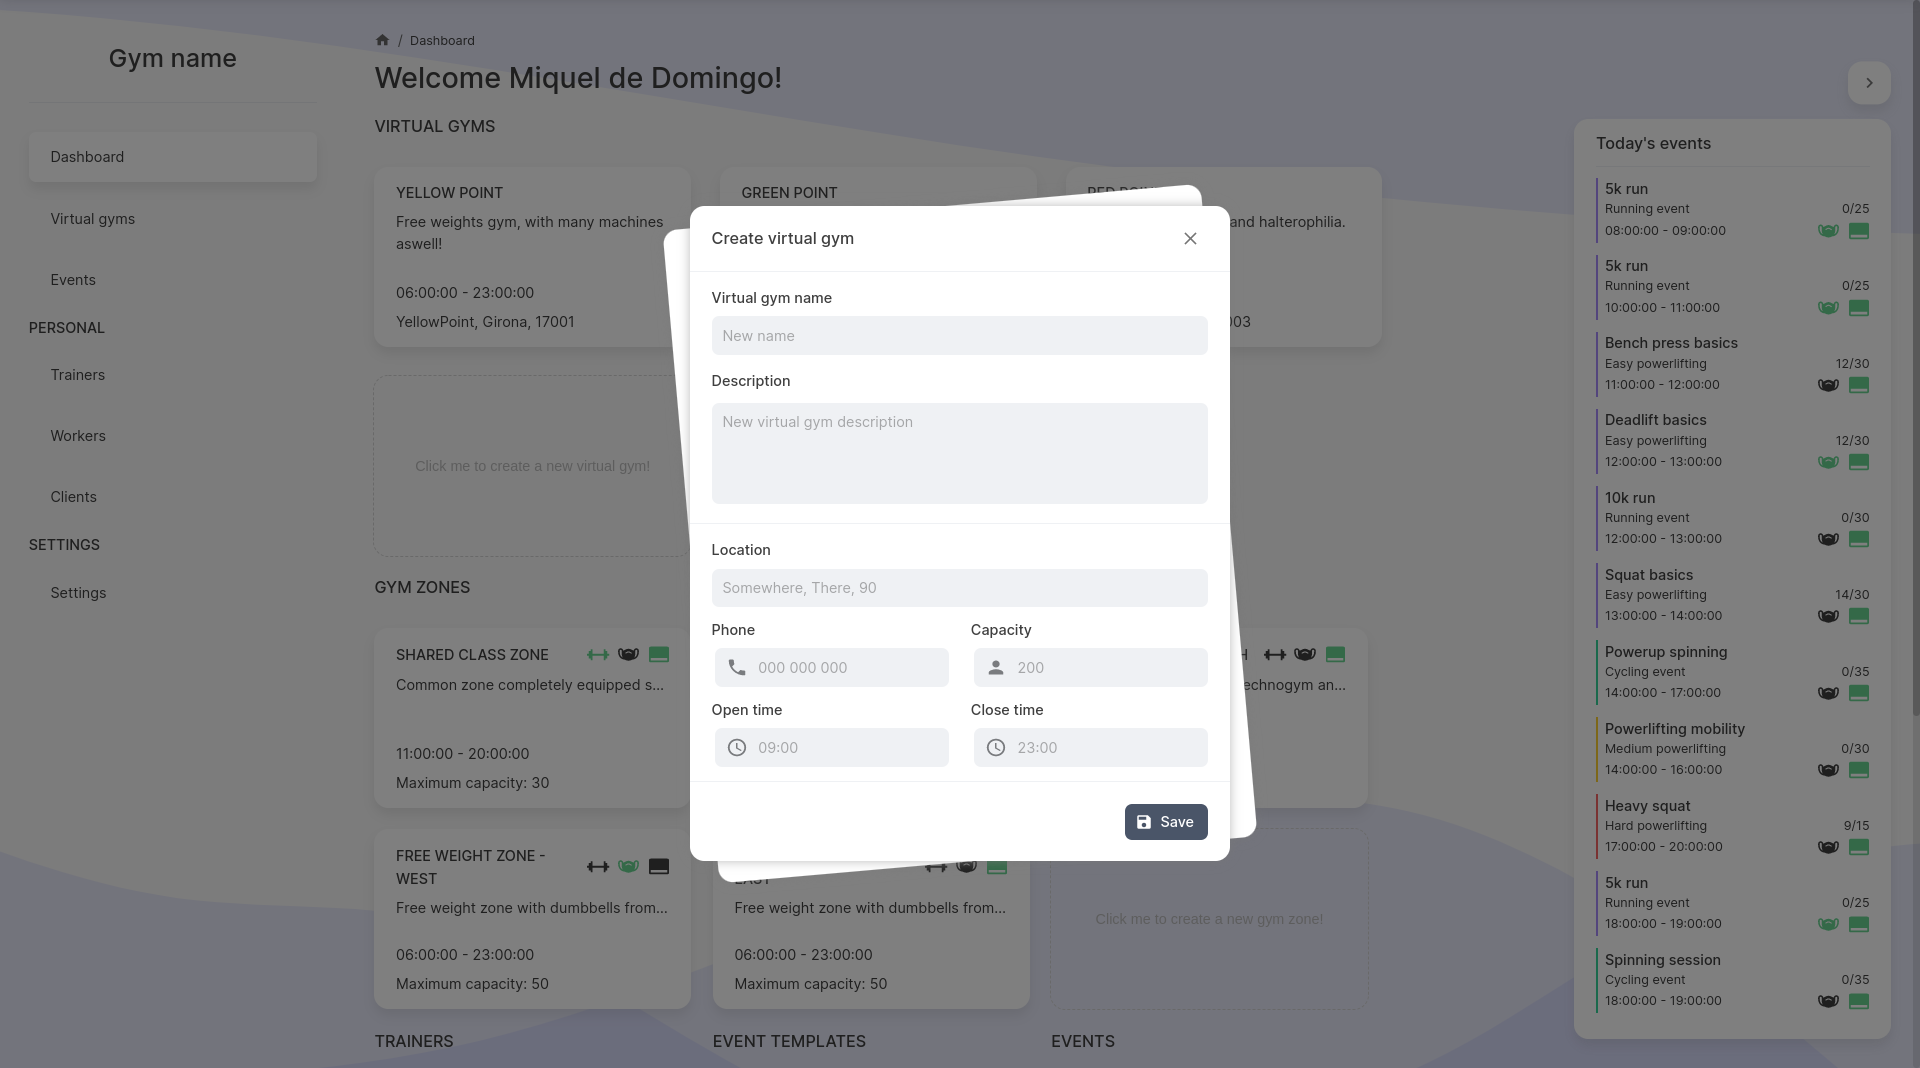
\includegraphics[width=\textwidth]{assets/core-screenshots/create-virtual-gym.png}
	\caption{Creation of a virtual gym}
\end{figure}
\subsubsection{Gym zone}
This view is only limited to the class type gym zones. That is becasue the non-class type do not have an events calendar.
\begin{figure}[H]
	\centering
	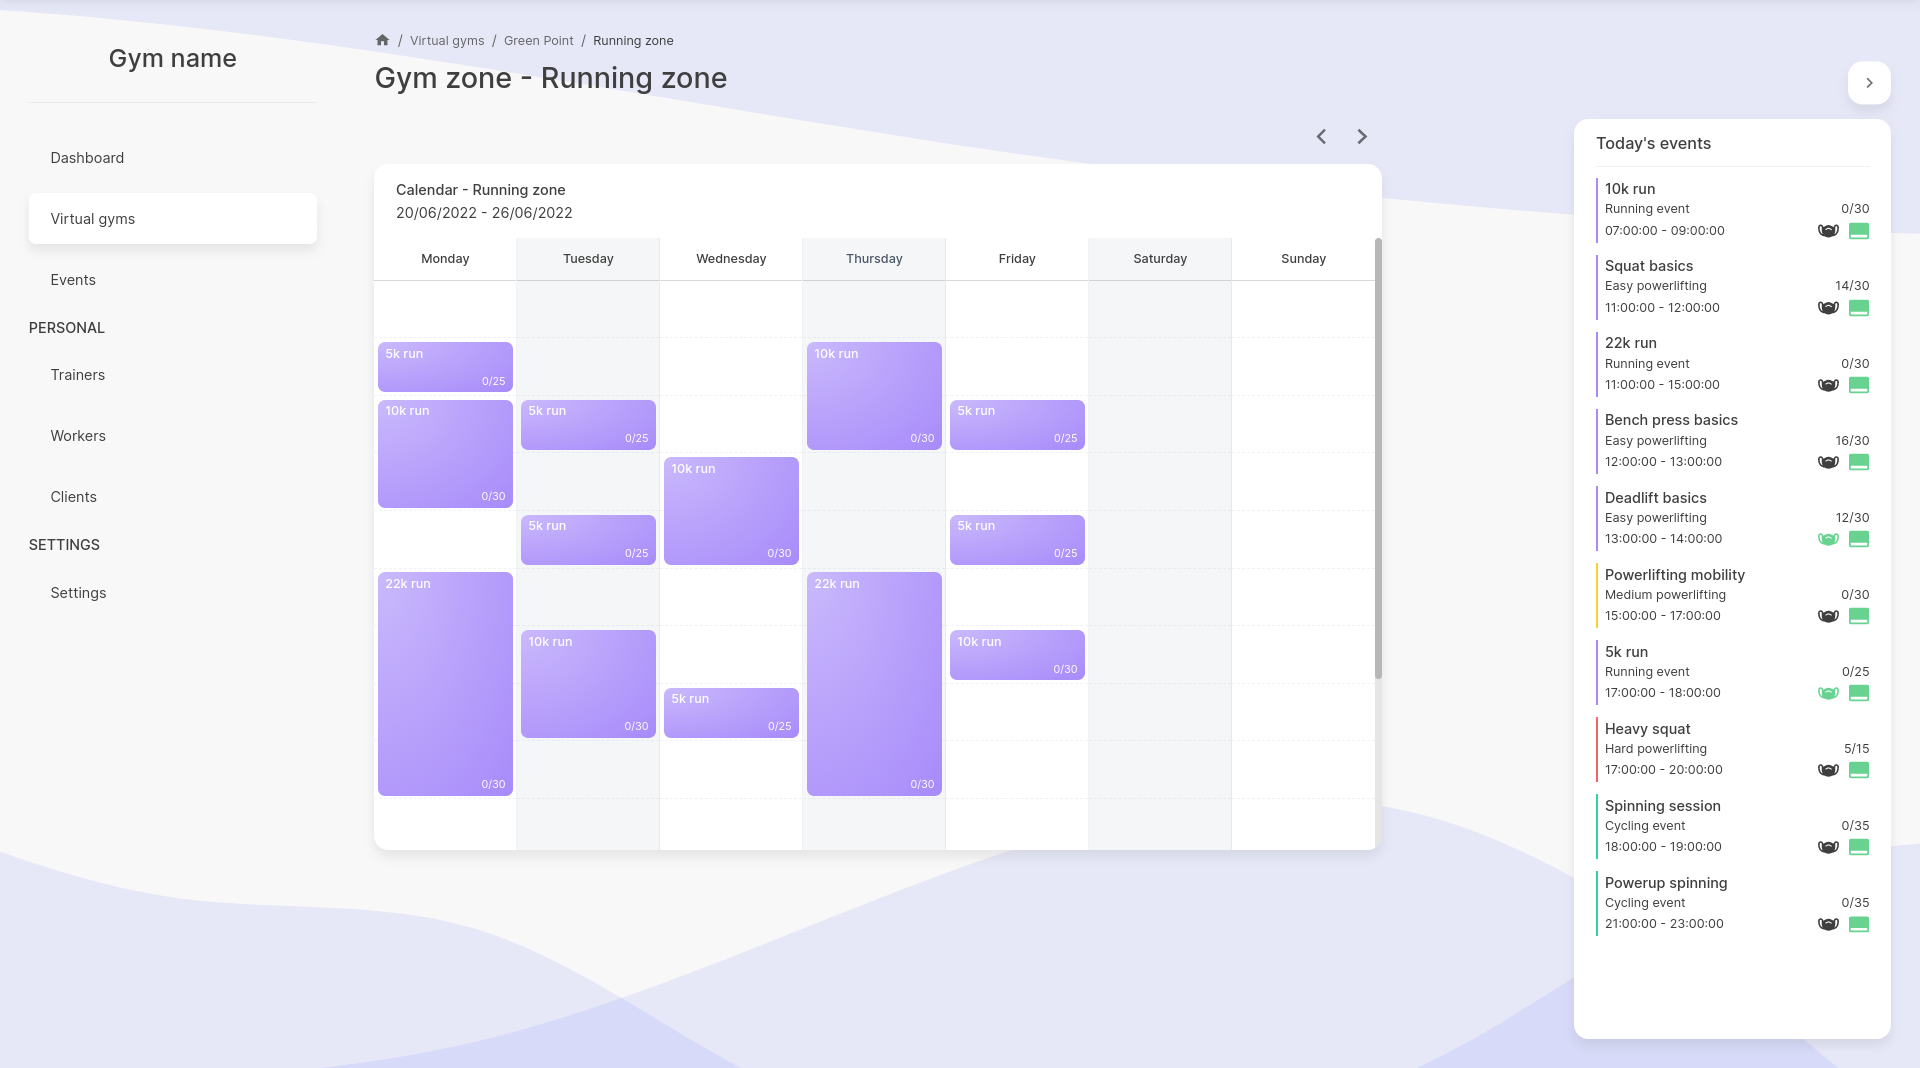
\includegraphics[width=\textwidth]{assets/core-screenshots/gym-zone-one.png}
	\caption{View of a calendar with events of the same event type}
\end{figure}
\begin{figure}[H]
	\centering
	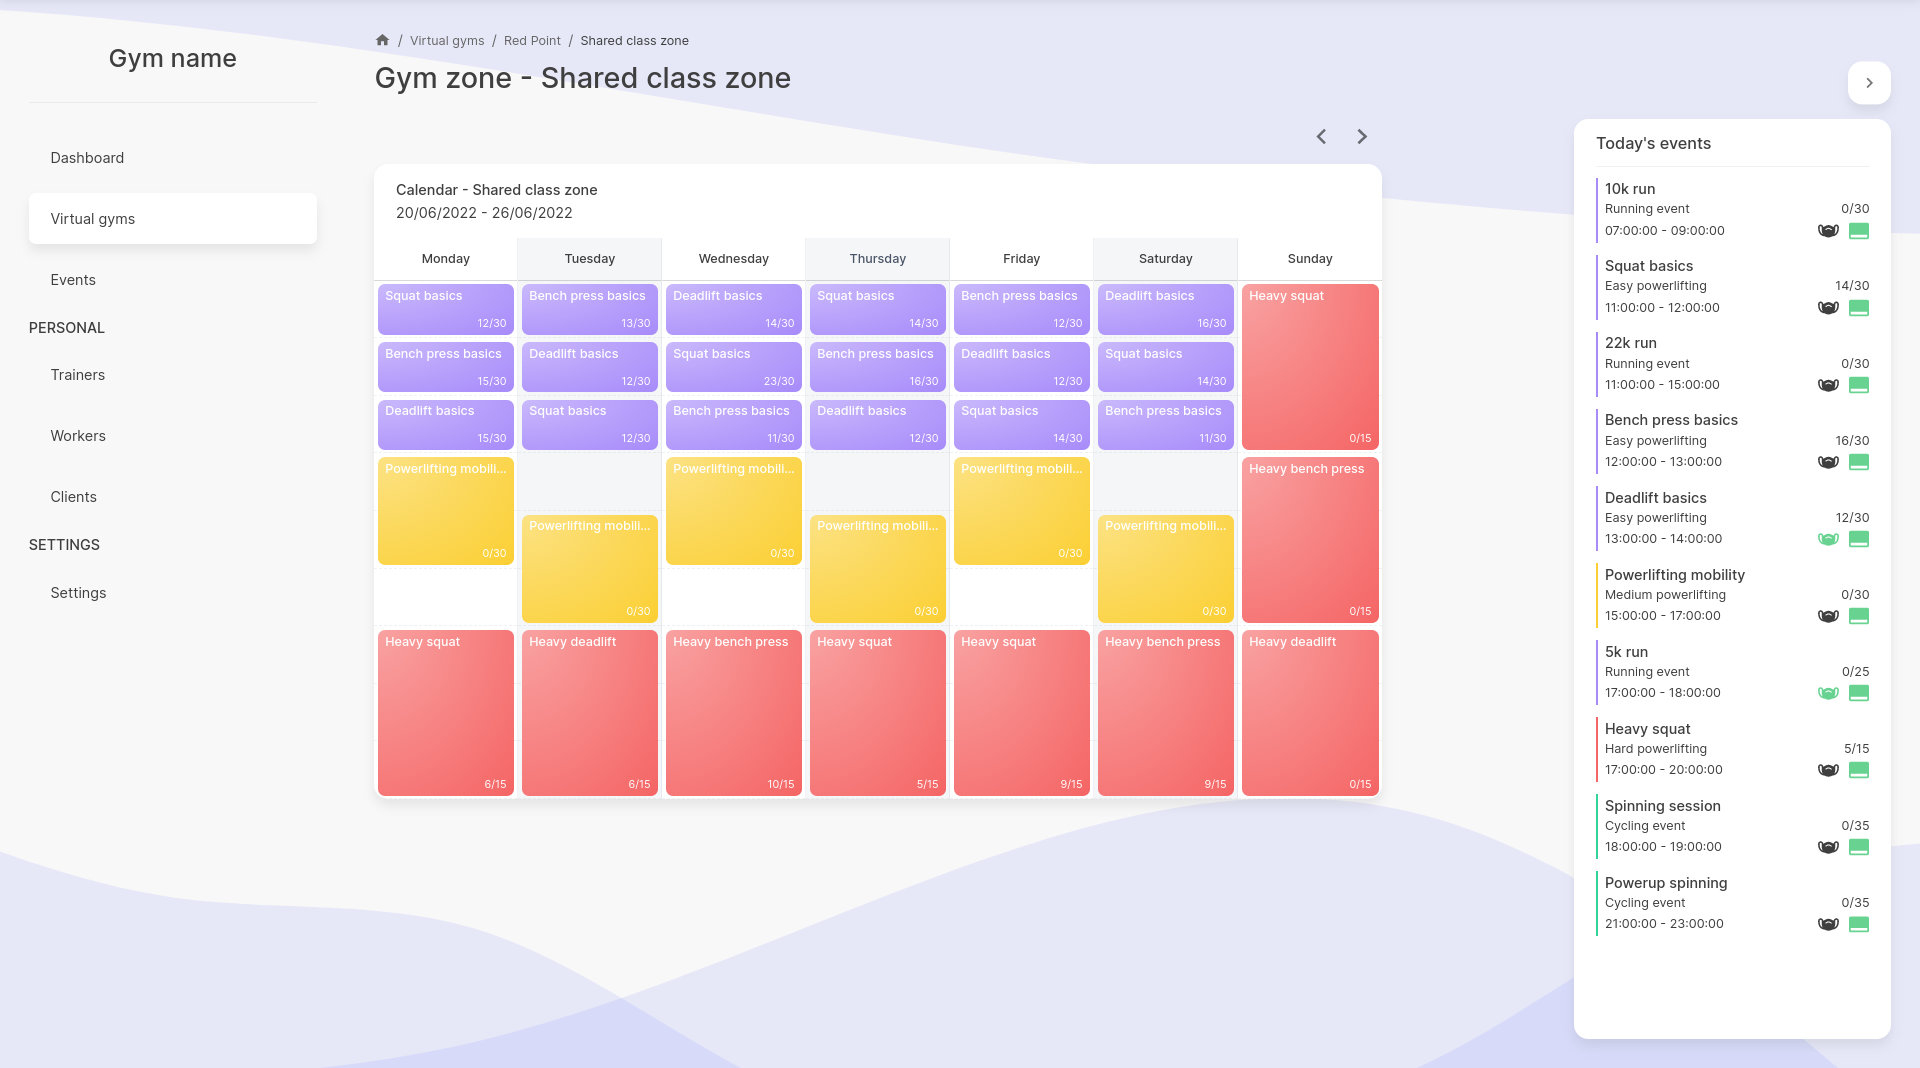
\includegraphics[width=\textwidth]{assets/core-screenshots/gym-zone-two.png}
	\caption{View of a calendar with events of different event type}
\end{figure}
Gym zones can be created from different views, which are the dashboard, the virtual gyms list page and the single virtual gym's page.
\begin{figure}[H]
	\centering
	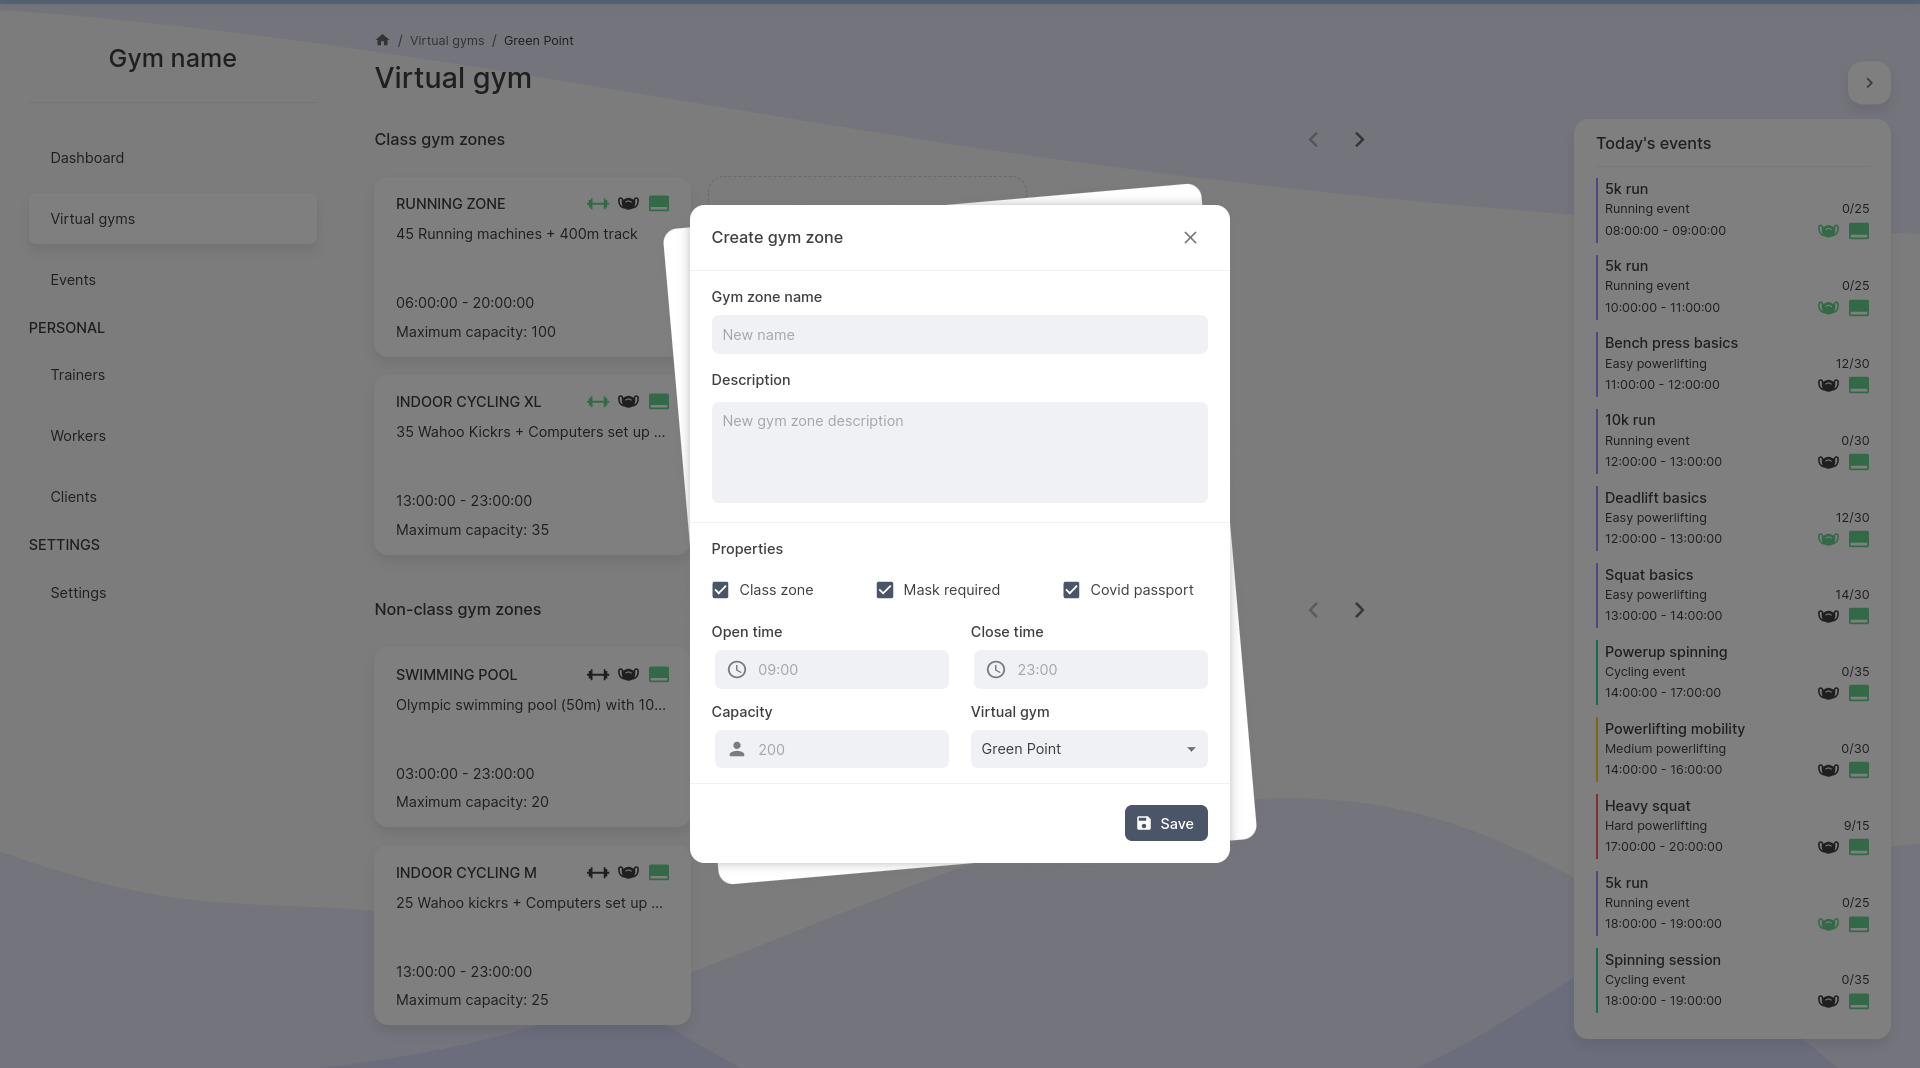
\includegraphics[width=\textwidth]{assets/core-screenshots/create-gym-zone.png}
	\caption{Virtual gym page}
\end{figure}
\begin{figure}[H]
	\centering
	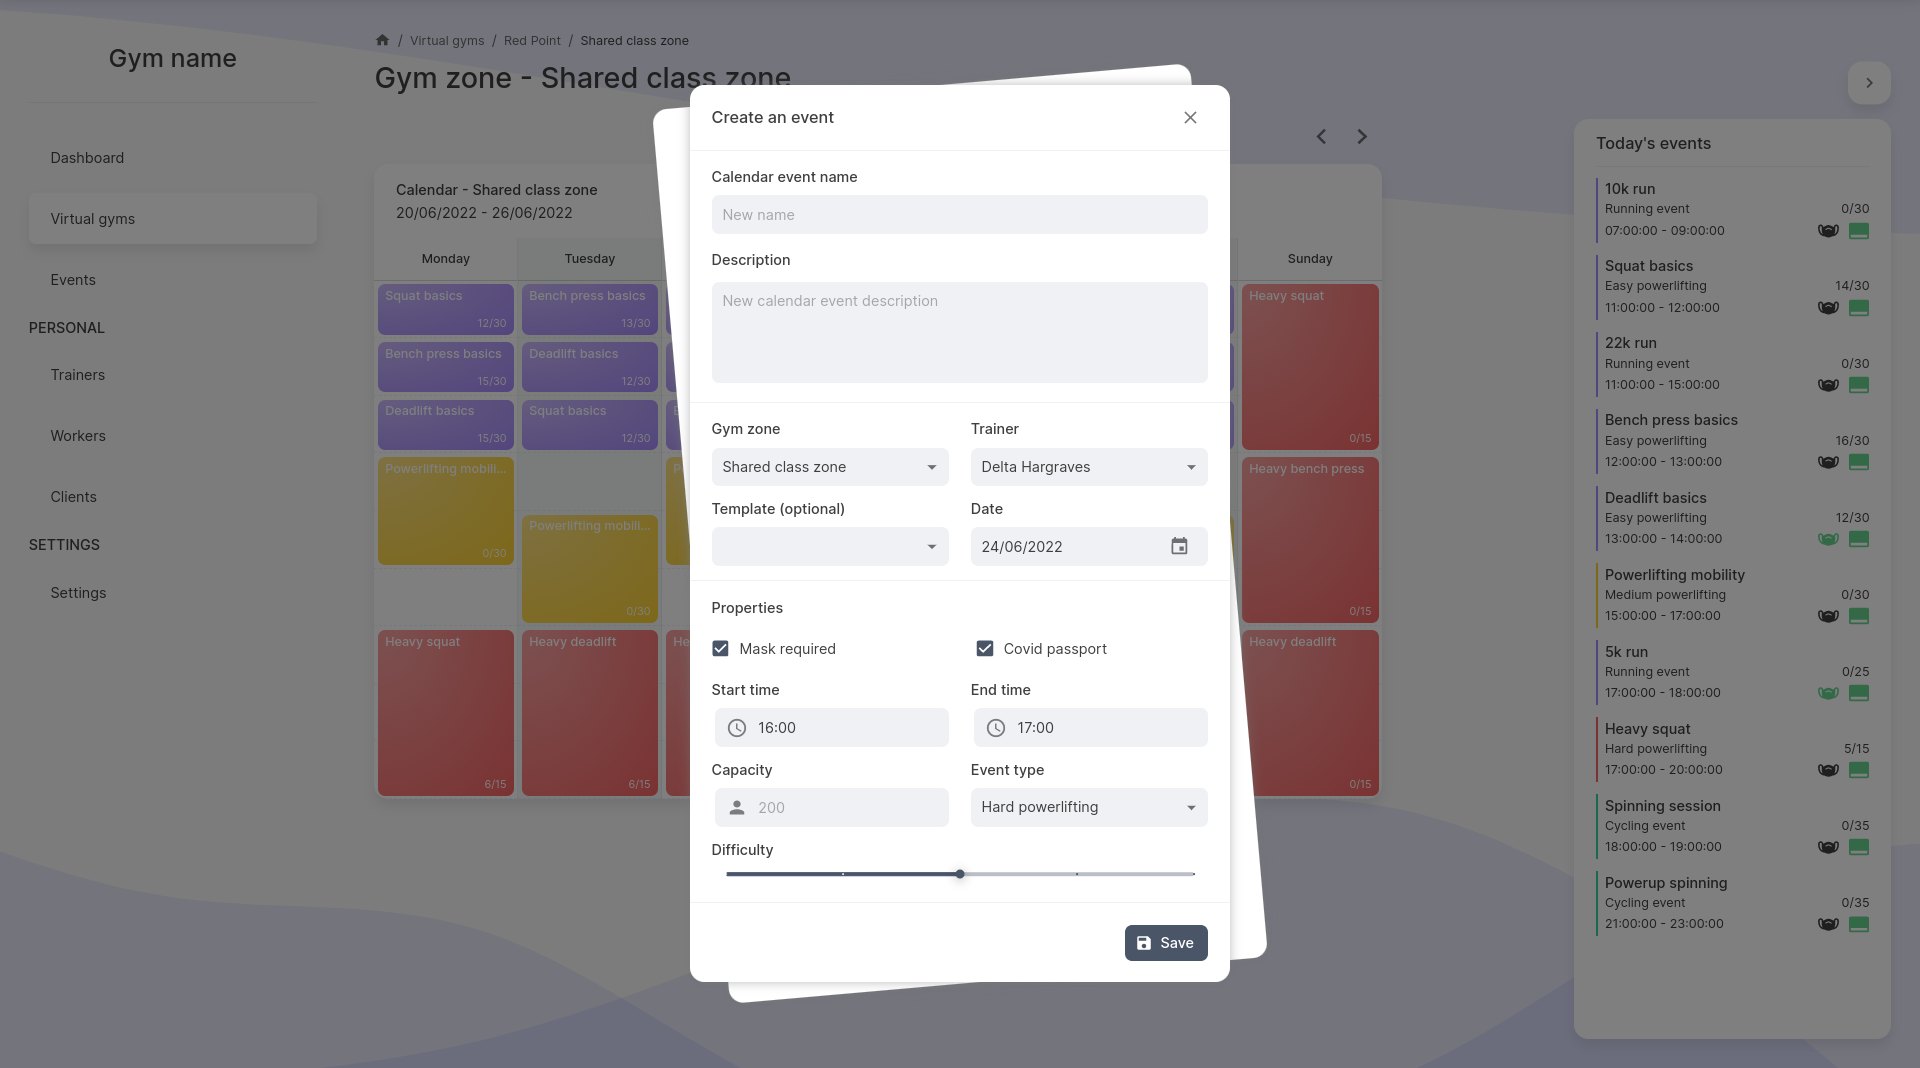
\includegraphics[width=\textwidth]{assets/core-screenshots/create-event.png}
	\caption{Creation of an event for a calendar}
\end{figure}
\subsubsection{Events}
\begin{figure}[H]
	\centering
	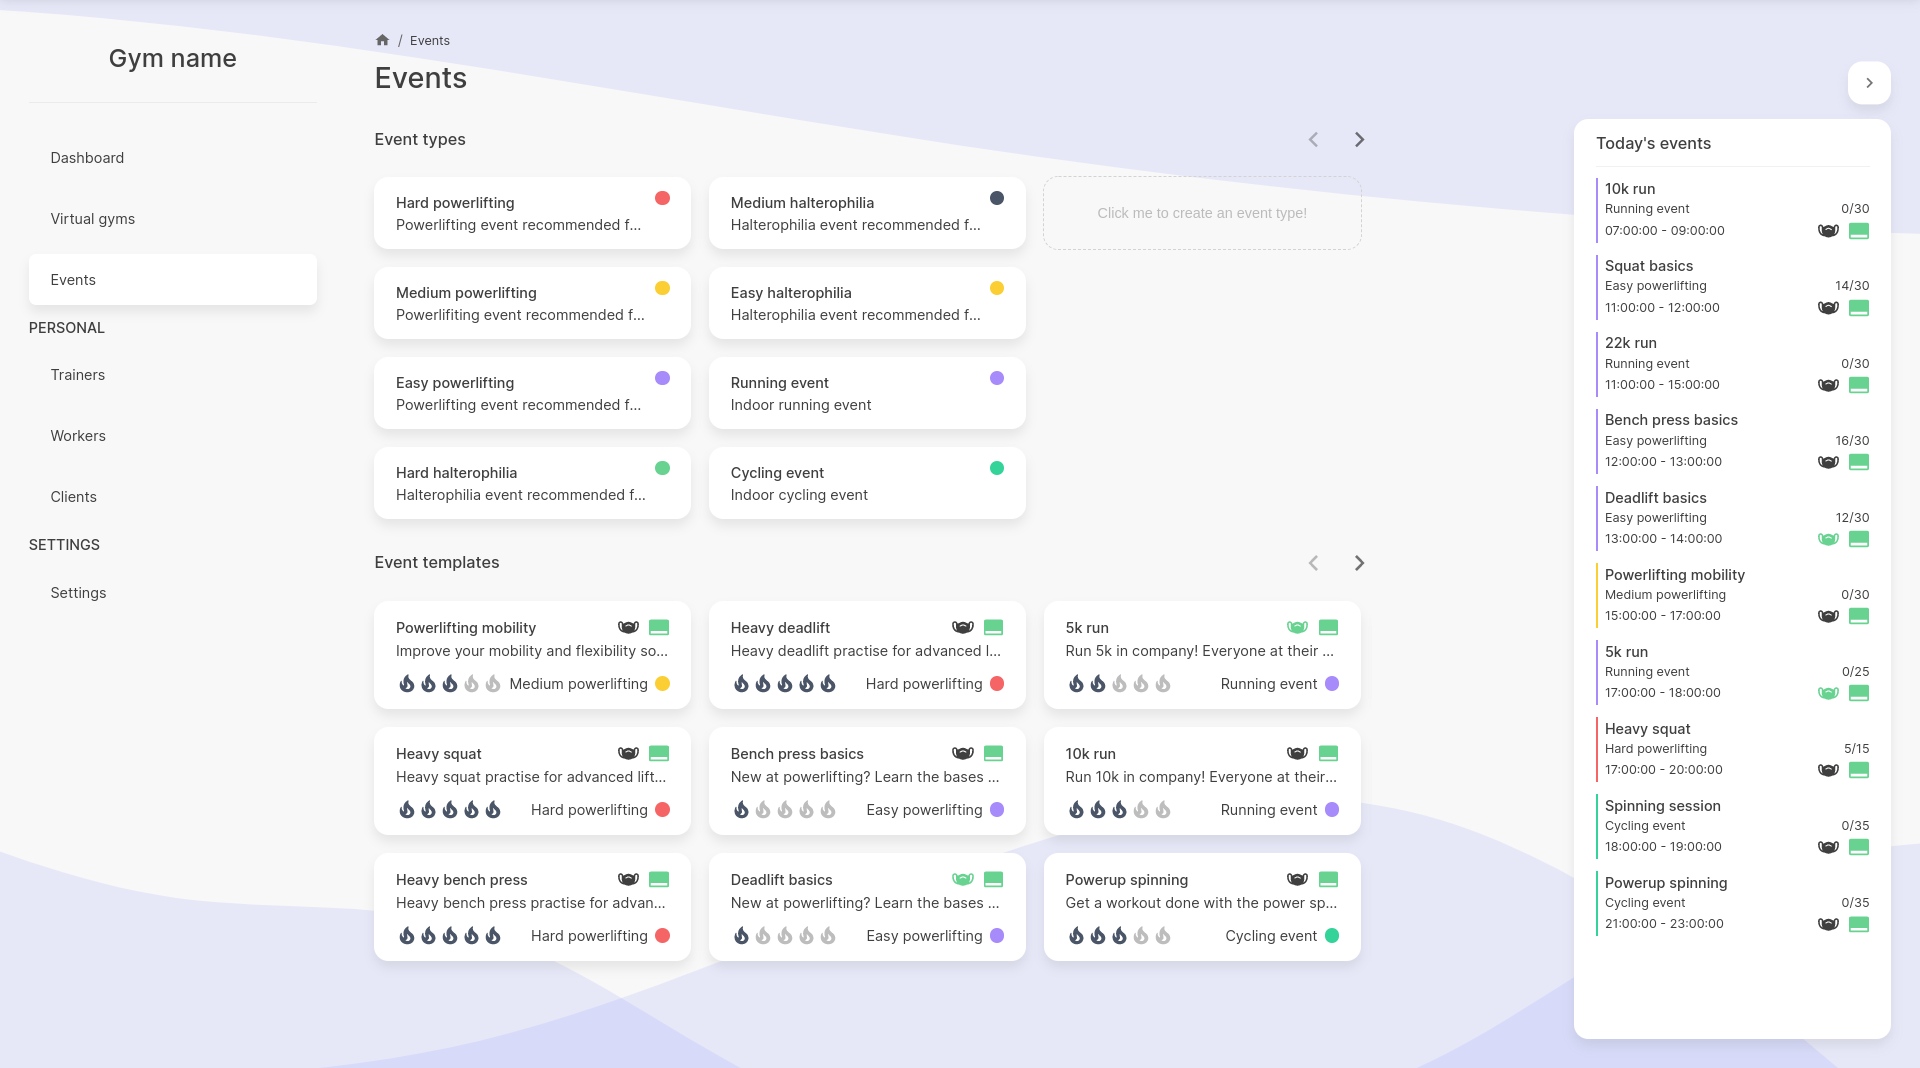
\includegraphics[width=\textwidth]{assets/core-screenshots/events.png}
	\caption{Events page with event types and event templates}
\end{figure}
\begin{figure}[H]
	\centering
	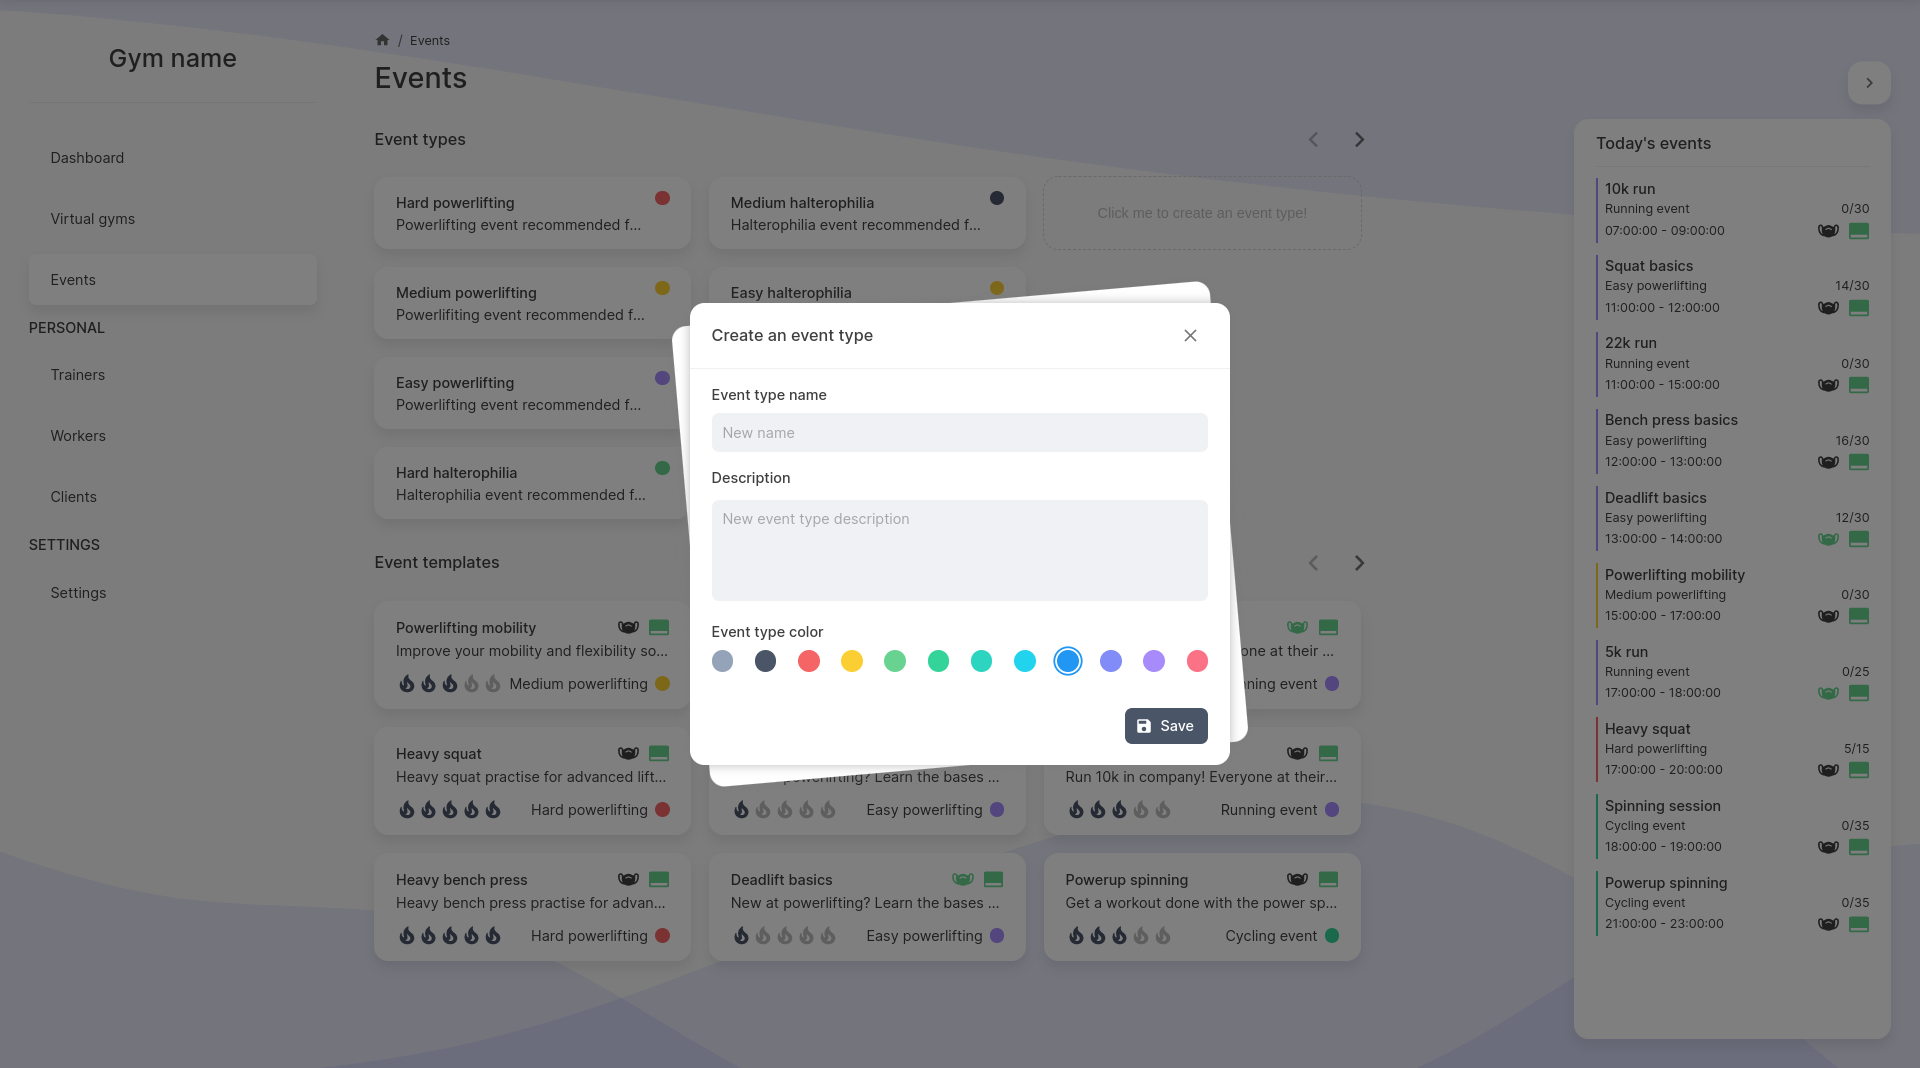
\includegraphics[width=\textwidth]{assets/core-screenshots/create-event-type.png}
	\caption{Creation of an event type}
\end{figure}
\begin{figure}[H]
	\centering
	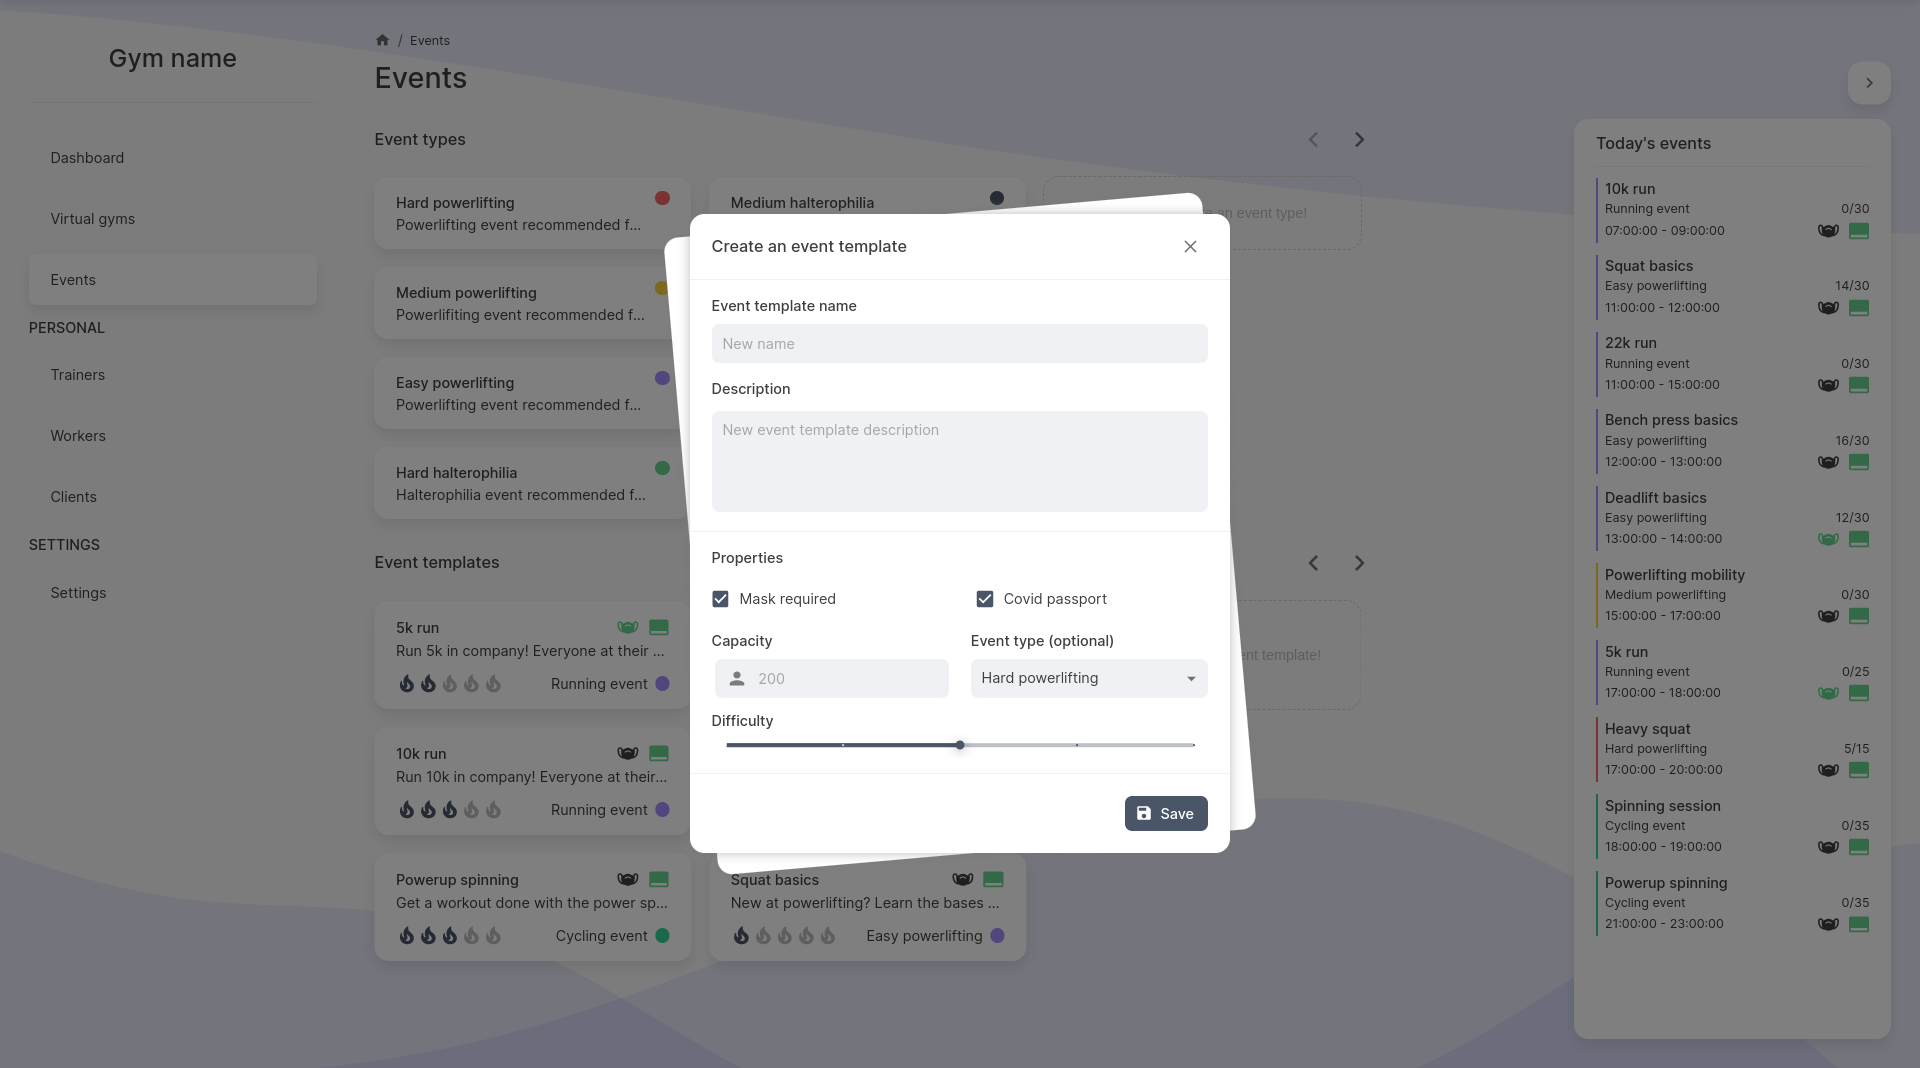
\includegraphics[width=\textwidth]{assets/core-screenshots/create-event-template.png}
	\caption{Creation of an event template}
\end{figure}
\subsubsection{Workers}
\begin{figure}[H]
	\centering
	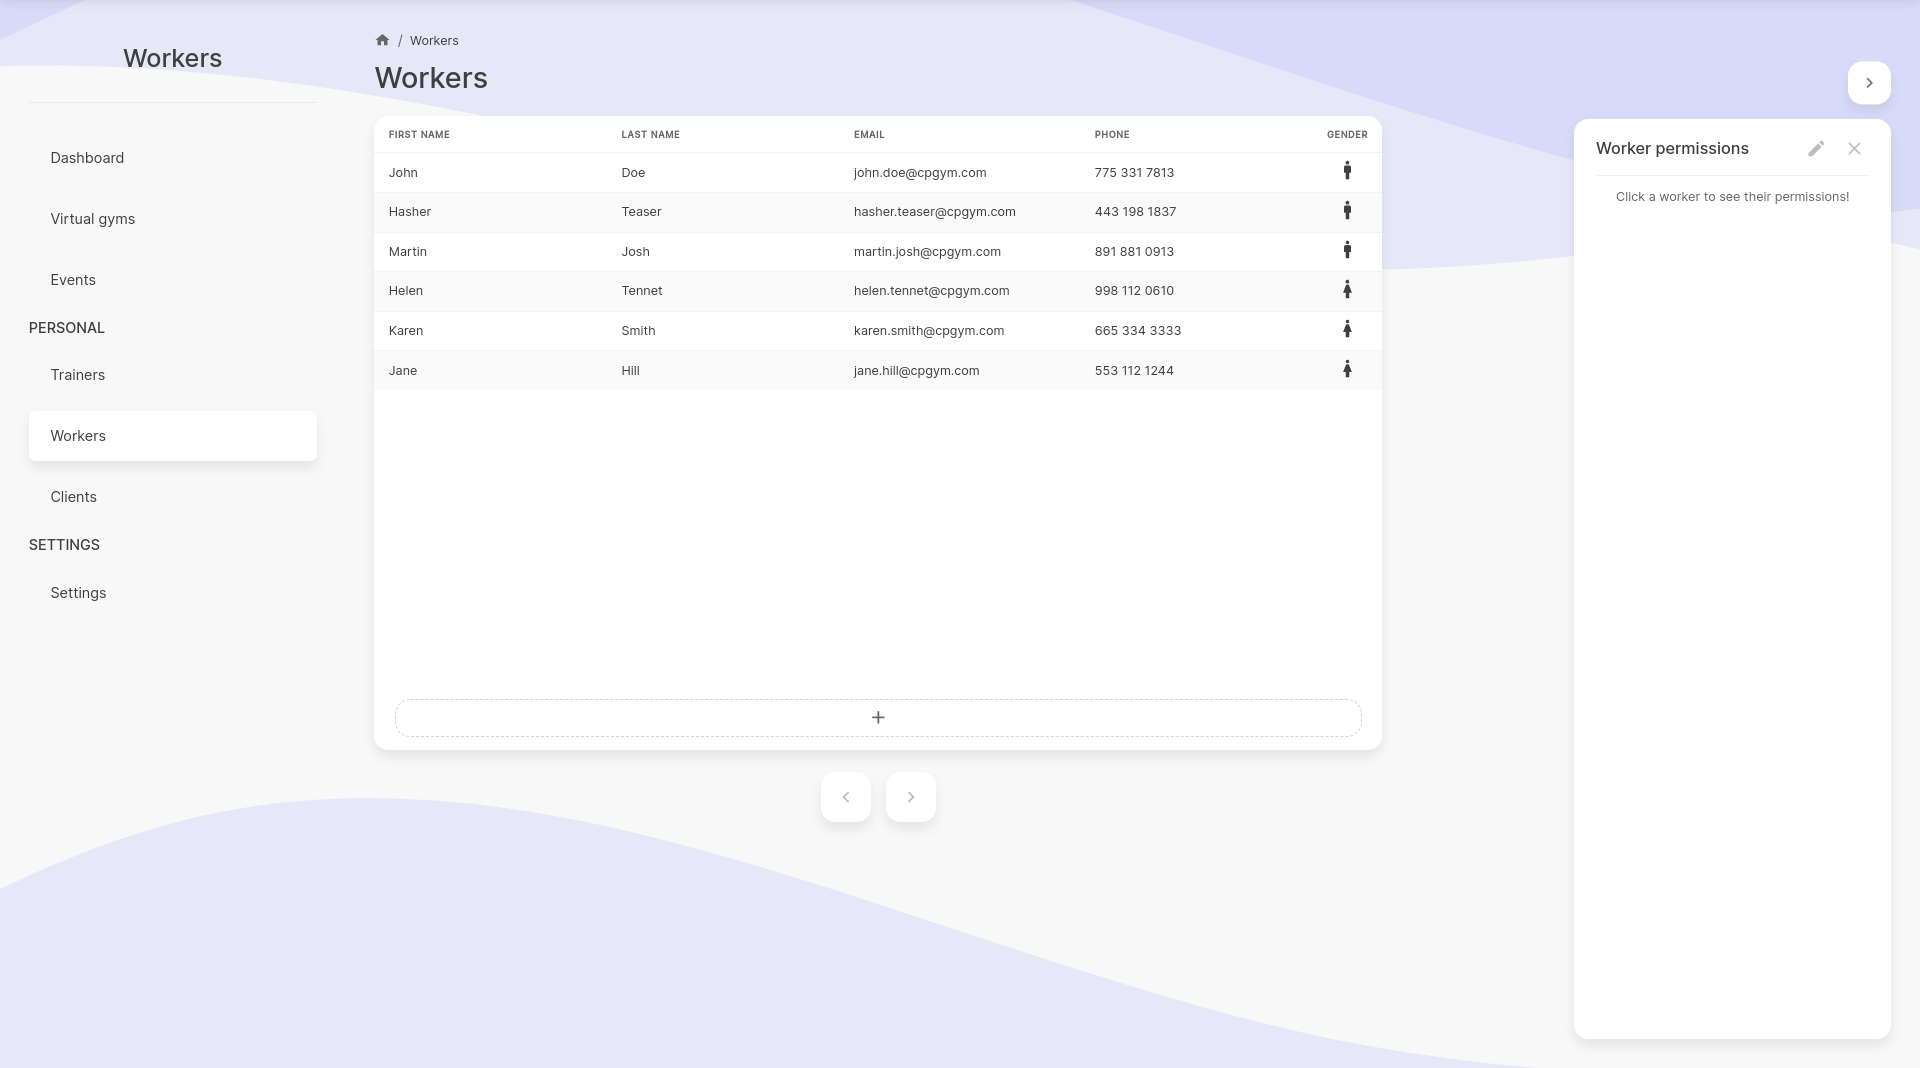
\includegraphics[width=\textwidth]{assets/core-screenshots/workers.png}
	\caption{Workers view without a worker selected}
\end{figure}
\begin{figure}[H]
	\centering
	\includegraphics[width=\textwidth]{assets/core-screenshots/workers-selected.png}
	\caption{Workers view with a worker selected}
\end{figure}
\begin{figure}[H]
	\centering
	\includegraphics[width=\textwidth]{assets/core-screenshots/create-worker.png}
	\caption{Creation of a worker}
\end{figure}
\subsubsection{Trainers}
\begin{figure}[H]
	\centering
	\includegraphics[width=\textwidth]{assets/core-screenshots/trainers.png}
	\caption{Trainers page}
\end{figure}
\begin{figure}[H]
	\centering
	\includegraphics[width=\textwidth]{assets/core-screenshots/create-trainer.png}
	\caption{Creation of a trainer}
\end{figure}
\subsubsection{Clients}
\begin{figure}[H]
	\centering
	\includegraphics[width=\textwidth]{assets/core-screenshots/clients.png}
	\caption{Clients page}
\end{figure}
\begin{figure}[H]
	\centering
	\includegraphics[width=\textwidth]{assets/core-screenshots/create-client.png}
	\caption{Creation of a client}
\end{figure}
\subsubsection{Settings}
The settings page for a worker would look the same, without having the gym properties available.
\begin{figure}[H]
	\centering
	\includegraphics[width=\textwidth]{assets/core-screenshots/settings.png}
	\caption{Settings page}
\end{figure}
\subsection{Client application}
\subsubsection{Authentication}
\begin{figure}[H]
	\centering
	\includegraphics[width=\textwidth]{assets/client-screenshots/sign-up.png}
	\caption{Sign up page}
\end{figure}
\begin{figure}[H]
	\centering
	\includegraphics[width=\textwidth]{assets/client-screenshots/log-in.png}
	\caption{Log in page}
\end{figure}
\subsubsection{Dashboard page}
In comparison to the core application, the dasboard page contains fewer actions, and it is more simple.
\begin{figure}[H]
	\centering
	\includegraphics[width=\textwidth]{assets/client-screenshots/dashboard.png}
	\caption{Dashboard page}
\end{figure}
\subsubsection{Virtual gyms}
\begin{figure}[H]
	\centering
	\includegraphics[width=\textwidth]{assets/client-screenshots/virtual-gyms.png}
	\caption{Virtual gyms page}
\end{figure}
Whenever a virtual gym has been clicked (by clicking at its name), the user is redirected to the above page, which displays all the gym zones of the chosen virtual gym.
\begin{figure}[H]
	\centering
	\includegraphics[width=\textwidth]{assets/client-screenshots/virtual-gym.png}
	\caption{Virtual gym page}
\end{figure}
\subsubsection{Gym zone}
\begin{figure}[H]
	\centering
	\includegraphics[width=\textwidth]{assets/client-screenshots/gym-zone.png}
	\caption{View of a gym zone}
\end{figure}
\subsubsection{Appointments}
\begin{figure}[H]
	\centering
	\includegraphics[width=\textwidth]{assets/client-screenshots/create-event-appointment.png}
	\caption{Creation of an appointment to an event}
\end{figure}
\begin{figure}[H]
	\centering
	\includegraphics[width=\textwidth]{assets/client-screenshots/event-appointment-created.png}
	\caption{Confirmation of an event appointment}
\end{figure}
\begin{figure}[H]
	\centering
	\includegraphics[width=\textwidth]{assets/client-screenshots/create-calendar-appointment.png}
	\caption{Creation of an appointment to a calendar}
\end{figure}
\begin{figure}[H]
	\centering
	\includegraphics[width=\textwidth]{assets/client-screenshots/calendar-appointment-created.png}
	\caption{Confirmation of a calendar appointment}
\end{figure}
\subsubsection{Settings}
\begin{figure}[H]
	\centering
	\includegraphics[width=\textwidth]{assets/client-screenshots/settings.png}
	\caption{Settings page}
\end{figure}
\chapter{Conclusions}
The goal of the project was to provide a tool that helped both gym owners to manage the appointments their clients made, durign the COVID restrictions. This objective has been accomplished with the Hubbl web application, which allows users to manage appointments in a gym environment. Nevertheless, it is hard to define an app as completely finished, as there may exist a bug that the developers have not seen, or the clients will require new features which will have to be implemented.
\\[8pt]
It is important to note that one of the objectives of the application was to provide an elegant and sofisticated user experience, at least better than my experience as a user of a similar software. Therefore, the Hubbl application not only provides value with its functionality, but also with the interface and use experience it ships with.
\\[8pt]
Furthermore, the Hubbl application tries to cover as many aspects as possible, while simplifying the usage of the application. As explained in the \emph{\nameref{future-work}} section, there are many other things to improve and to add as new features. Nonetheless, the version that is provided has more than what the app is expected to do. Due to the lack of time, inexpertise in some fields or tools used, and the fact that I have only been developing the application, it has not been possible to develop all that was expected for the wanted deadlines.
\\[8pt]
The project has required me to use pieces of knowledge acquired in the degree. At the same time, I have been pushed outside my comfort zone, dedicating time to reading documentation pages and similar.
\\[8pt]
To sum up, the project has provided a sense of how difficult and complex can it be from brainstorming the idea of the application, to finding the proper architecture to later develop it.
\chapter{Future work}
\label{future-work}
It is barely ever true that a software application can be considered as \emph{finished}. Few are the cases in which the software does not need further development. The Hubbl application it will require of improvements and the addition of new features, so that the clients see more value in the organisation and application. Such thing is extremely common in product-bases software. Therefore, in general terms, the \emph{maintenance} and \emph{improvement} of the software will be the future work itself.
\\[8pt]
Aside from the general points, due to the lack of time and handwork (being me the only developer) it has not been possible to fulfill all the functional requirements. The following list contains what is left to be done:
\begin{enumerate}[label = -]
	\item \emph{Appointments}. Currently, it is not possible to view the list of appointments for an event or a gym zone. Therefore, the gym owner or any worker, are not able to see who is attending the gym zone\footnote{In the case of the events, it is possible to see how many clients have made an appoitment, yet it is not possible to know who.}. It is the same for the clients, they are not able to see their past and future appointments.
	      \newline
	      In the left navigation bar, a new tab will be added in both applications (core and client) which will allow the user to see the appointments made. In the case of the core application, it will display all the appointments made, while allowing the user to filter (by name, gym zone, event, event type and so on). Such view will require an enourmous amount of time for a singe developer to develop.
	\item \emph{Archival}. Archiving gym zones, events, clients and any item that can be deleted would allow the user to soft-delete items, meaning that such items could be recovered in the future. Currently, the server only supports hard-deletion, the opposite, as it requires less logic in the backed. However, the goal would be to provide the user with both utilities, being able to permanently remove or temporarily remove items.
	\item \emph{Update gym zones and virtual gyms}. It is currently not possible to edit the characteristics (name, description, open and close time, and so on) of a virtual gym nor a gym zone. I have not found the best place, in terms of user expercience, to locate such edition. Therefore, I have kept \emph{procastinating} the task, yet it would have a high priority in comparison to other tasks.
	\item \emph{Filtering}. The woker, trainer and client views will contain a lot of data which can be hard to visualise sometimes. That is the reason why providing filters for such views will add enourmous value to such features.
	\item \emph{Analytics}. Alongside the archiving feature, having analytics of the gym would provide tremendous value to the gym owner and their coworkers, but it requires a vast amount of time to be developed. Therefore, as I have stated in the \emph{\nameref{functional-requirements}} section, it was already something that I knew I wouldn't have time to develop, and it would be a \emph{nice-to-have} for the user. Such feature whould be added as another tab in the lateral menu, and it would only be accessible to the gym owner and to the workers with permissions to view them.
	\item \emph{Light/Dark theme}. It is currently possible in the server to change the theme from light to dark and vice-versa. However, since I did not have enought time to define a dark system design, I opted not to add it in the client. Nonetheless, it should be an easy to add feature, as the \emph{mui} library provides an easy tool for such feature.
	\item \emph{Client e2e}. Again, due to the lack of time and handwork, I have not been able to develop end-to-end tests for the client applications. I have little experience with developing such tests, and I would have required a vast amount of time to code consistent and valuable end-to-end tests.
	\item \emph{Deployment}. Finally, I would have wanted to deploy the applications to a web server so that they would be accessible to anyone. Such thing will not be possible until the application includes most of the above points, excluding analytics and archival.
\end{enumerate}
To sum up, even though the list may seem large, the application is fully functional and provides the basic utilities for the owners, workers and clients to properly organise themselves.
\begin{thebibliography}{9}
	% Autor. Any de l’última actualització. Títol en cursiva. Dia mes any consulta. URL
	\bibitem{salary-one}
	Unspecified author. Unspecified last update. \emph{Salario medio para Diseñador Ui en España, 2022}. April 19th 2022. \url{https://es.talent.com/salary?job=dise%C3%B1ador+ui}.
	\bibitem{salary-two}
	Unspecified author. Unspecified last update. \emph{Salario medio para Programador Javascript en España, 2022}. April 19th 2022. \url{https://es.talent.com/salary?job=programador+javascript}.
	\bibitem{jira}
	Atlassian. Unspecified last update. \emph{Jira Software homepage}. March 20th 2022. \url{https://www.atlassian.com/software/jira}.
	\bibitem{jira-smart-commits}
	Unspecified author. Unspecified last update. \emph{Use smart commits}. March 20th 2022. \url{https://support.atlassian.com/bitbucket-cloud/docs/use-smart-commits/}.
	\bibitem{nx}
	Unspecified author. Unspecified last update. \emph{Using Nx at Enterprises}. December 12th 2021. \url{https://nx.dev/l/r/guides/monorepo-nx-enterprise#apps-and-libs}.
	\bibitem{nextjs}
	Vercel. Unspecified last update. \emph{The React Framework for Production}. December 12th 2021. \url{https://nextjs.org/}.
	\bibitem{code-splitting}
	MDN contributors. January 28th 2022. \emph{Code splitting}. December 12th 2021. \url{https://developer.mozilla.org/en-US/docs/Glossary/Code_splitting}.
	\bibitem{mui}
	Unspecified author. Unspecified last update. \emph{Move faster with intuitive React UI tools}. December 12th 2021. \url{https://mui.com/}.
	\bibitem{postgresql}
	Unspecified author. Unspecified last update. \emph{PostgresQL: The World's Most Advanced Open Source Relational Database}. December 12th 2021. \url{https://www.postgresql.org/}.
	\bibitem{expressjs}
	Unspecified author. Unspecified last update. \emph{4.x API}. December 13th 2021. \url{https://expressjs.com/en/api.html}.
	\bibitem{typeorm}
	\texttt{@pleerock}\footnote{GitHub's username.}. April 28th 2022. \emph{\texttt{typeorm/typeorm}}. December 13th 2021. \url{https://github.com/typeorm/typeorm}.
	\bibitem{jest}
	Facebook. Unspecified last update. \emph{Jest}. December 13th 2021. \url{https://expressjs.com/en/api.html}.
	\bibitem{react-testing-library}
	\texttt{@Nick McCurdy}\footnote{GitHub's username.}. September 21st 2021. \emph{React Testing Library}. December 13th 2021. \url{https://testing-library.com/docs/react-testing-library/intro}.
	\bibitem{cypress}
	Cypress.io. Unspecified last update. \emph{Javascript End to End testing framework}. December 13th 2021. \url{https://www.cypress.io/}
	\bibitem{github-workflows}
	Unspecified author. Unspecified last update. \emph{Using workflows}. May 22nd 2022. \url{https://docs.github.com/en/actions/using-workflows}
\end{thebibliography}
\end{document}